\documentclass{article}
\usepackage[utf8]{inputenc}
\usepackage{amsmath, amssymb, amsfonts, amsthm}
\usepackage{mathtools}
\usepackage{mdframed}
\usepackage{cancel}
\usepackage{import, xifthen, pdfpages, transparent}
\usepackage{enumitem}
\usepackage{geometry}
\usepackage{multicol}
\usepackage{hyperref}
\usepackage{float}
\usepackage{tikz, pgfplots}
\usetikzlibrary{positioning}
\pgfplotsset{compat=1.18}
\geometry{a4paper, margin=2cm}

\newmdenv[
  linecolor=black,
  linewidth=1pt,
  roundcorner=5pt,
  innertopmargin=4pt,
  innerbottommargin=10pt,
  innerleftmargin=10pt,
  innerrightmargin=10pt
]{bxthm}

\theoremstyle{plain}
\newtheorem{thm}{Teorema}[section]
\newtheorem{lem}[thm]{Lemma}
\newtheorem{prop}[thm]{Proposizione}
\newtheorem{cor}{Corollario}

\theoremstyle{definition}
\newtheorem{defn}{Definizione}[section]
\newtheorem{exmp}{Esempio}[section]
\newtheorem{xca}[exmp]{Esercizio}

\theoremstyle{remark}
\newtheorem{rem}{Osservazione}
\newtheorem{note}{Nota}
\newtheorem{case}{Caso}

\newcommand{\incfig}[2][\columnwidth]{%
    \def\svgwidth{#1}
    \import{./figures/}{#2.pdf_tex}
}


\begin{document}
\begin{titlepage}
    \centering
	{\textsc{Università degli Studi della Basilicata} \par}
	\vspace{2cm}
    {\huge\bfseries Analisi I\par}
    \vfill
	{\Large\itshape Donato Martinelli\par}
	{\large \today\par}
\end{titlepage}

\tableofcontents

\vspace{50pt}
\part{Insiemi e Numeri}
\vspace{50pt}
\section{I Numeri Reali}
\vspace{50pt}

\subsection{Il sistema dei numeri reali}
\vspace{10pt}

Gli assiomi dei numeri reali si possono classificare in tre gruppi:
\begin{enumerate}
    \item[(a)] \textbf{Assiomi di campo}, riguardanti le operazioni che si possono eseguire tra numeri reali;
    \item[(b)] \textbf{Assiomi di ordine}, relative alla possibilità di confrontare tra loro i numeri reali per identificarne il “maggiore”;
    \item[(c)] \textbf{Assioma di completezza}.
\end{enumerate}
A partire da questi assiomi dedurremo tutte le altre proprietà dei numeri reali.

\vspace{10pt}
\paragraph{Assiomi di campo}
\vspace{10pt}

Nell'insieme $\mathbb{R}$ sono definite due operazioni, l'addizione e la moltiplicazione definite rispettivamente al seguente modo:
\[+:\mathbb{R}\times \mathbb{R}\to \mathbb{R}\quad (a,b)\mapsto a+b\quad\quad\cdot:\mathbb{R}\times \mathbb{R}\to \mathbb{R}\quad (a,b)\mapsto a\cdot b=ab.\]
tali che valgono i seguenti assiomi:
\begin{itemize}
    \item[] \textbf{Assioma 1 (Associatività)}
    \[\forall\,a,b,c\in\mathbb{R},\quad(a+b)+c=a+(b+c)\quad\land\quad (ab)c=a(bc);\] 
    \item[] \textbf{Assioma 2 (Commutatività)}
    \[\forall\,a,b\in\mathbb{R},\quad a+b=b+a \quad\land\quad ab=ba;\]
    \item[] \textbf{Assioma 3 (Distributività)}
    \[\forall\,a,b,c\in\mathbb{R},\quad a(b+c)=ab+ac;\] 
    \item[] \textbf{Assioma 4 (Esistenza degli elementi neutri)}
    \[\exists\,z,v\in\mathbb{R}\;(z\neq v)\,:\;\forall\,a\in\mathbb{R},\quad a+z=a\quad\land\quad a\cdot v=a\]
    \item[] \textbf{Assioma 5 (Esistenza dell'opposto)}
    \[\forall\,a\in\mathbb{R},\;\exists\,\bar{a}\in\mathbb{R}\,:\;a+\bar{a}=0\]
    \item[] \textbf{Assioma 6 (Esistenza dell'inverso)}
    \[\forall\,a\in\mathbb{R}-\{0\},\;\exists\,\tilde{a}\in\mathbb{R}\,:\;a\cdot\tilde{a}=1\]
    con \[\tilde{a}=a^{-1}=\dfrac{1}{a}.\]
\end{itemize}

\vspace{10pt}

\paragraph{Unicità dell'elemento neutro per l'addizione}
\begin{bxthm}
\begin{prop}
    L'elemento neutro per l'addizione $z$ di cui all'assioma $4$, è unico e lo chiamiamo $0$.
\end{prop}
\end{bxthm}
\begin{proof}
    Siano $z',z''\in\mathbb{R}$ tali che 
    \begin{enumerate}
        \item $\forall\,a\in\mathbb{R},\quad a+z'=a$
        \item $\forall\,a\in\mathbb{R},\quad a+z''=a$
    \end{enumerate}
    Da (1), ponendo $a=z''$,  abbiamo che 
    \[z'' + z' = z''\]
    mentre da (2), ponendo $a=z'$ abbiamo che 
    \[z' + z'' = z'.\] 
    Per la commutatività dell'addizione, abbiamo 
    \[z' = z'+z'' = z''+z' = z''\]
    da cui ricaviamo
    \[z'=z''.\]
\end{proof}

\vspace{10pt}

\paragraph{Unicità dell'elemento opposto per l'addizione}
\begin{bxthm}
\begin{prop}
    Per ogni $a\in\mathbb{R}$, l'elemento opposto $\bar{a}$ di cui all'assioma $5$, è unico e lo chiamiamo $-a$.
\end{prop}
\end{bxthm}
\begin{proof}
    Siano $\bar{a},\bar{\bar{a}}\in\mathbb{R}$ tali che 
    \[\forall\,a\in\mathbb{R},\quad a+\bar{a}=0\;\land\;a+\bar{\bar{a}}=0\]
    allora abbiamo 
    \[\bar{a}=\bar{a}+0=\bar{a}+(a+\bar{\bar{a}})=(\bar{a}+a)+\bar{\bar{a}}=0+\bar{\bar{a}}=\bar{\bar{a}}.\]
\end{proof}

\vspace{10pt}

\paragraph{Legge di annullamento del prodotto}
\begin{bxthm}
\begin{prop}
    \[\forall\,a\in\mathbb{R},\quad a\cdot0=0.\]
\end{prop}
\end{bxthm}
\begin{proof}
    \[a\cdot0=a\cdot0 + (a\cdot0+(-a\cdot0))=(a\cdot0 + a\cdot0)+(-a\cdot0)=a\cdot(0 + 0)+(-a\cdot0)=a\cdot0+(-a\cdot0)=0.\]
\end{proof}

\vspace{10pt}
\paragraph{Assiomi di ordine}
\vspace{10pt}

Su $\mathbb{R}$ si introduce una relazione d'ordine a partire dal concetto non definito di \textit{positività}.
Esiste $\mathbb{R}^+\subseteq\mathbb{R}$, detto insieme dei numeri reali \textit{positivi} che soddisfa i due assiomi seguenti:

\vspace{10pt}

\begin{itemize}
    \item[] \textbf{Assioma 7}
    \[\forall\,a,b\in\mathbb{R}^+,\quad a+b,\,ab\in\mathbb{R^+};\] 
    \item[] \textbf{Assioma 8}
    \[\forall\,a\in\mathbb{R},\quad a=0\;\lor\;a\in\mathbb{R}^+\;\lor\;-a\in\mathbb{R}^+;\]
\end{itemize}

\vspace{10pt}

\begin{bxthm}
\begin{defn}
    Definiamo una relazione $<$ in $\mathbb{R}$ ponendo 
    \begin{align*}
        x<y\;\lor\;y>x &\iff \exists\,\varepsilon\in\mathbb{R}^+\,:\;x+\varepsilon=y;\\
        x\leq y \;\lor\;y\geq x&\iff x<y\;\lor\;x=y.
    \end{align*}
    Possiamo dunque definire i seguenti insiemi
    \[\mathbb{R}^+=\{x\in\mathbb{R}\,:\;x>0\} \quad \mathbb{R}^-=\{x\in\mathbb{R}\,:\;x<0\}.  \]
\end{defn}
\end{bxthm}

\vspace{10pt}

\begin{bxthm}
\begin{thm}
    La relazione $\leq$ è una relazione d'ordine totale su $\mathbb{R}$. In altri termini essa soddisfa le seguenti proprietà:
    \begin{itemize}
        \item[$a$] \textit{riflessività}: 
        \[\forall\,a\in\mathbb{R},\quad a\leq a,\]
        \item[$b$] \textit{antisimmetria}: 
        \[\forall\,a,b\in\mathbb{R},\quad a\leq b\;\land\; b\leq a \implies a=b,\]
        \item[$c$] \textit{transitività}:
        \[\forall\,a,b,c\in\mathbb{R},\quad a\leq b\;\land\; b\leq c \implies a\leq c,\]
        \item[$d$] \textit{totalità}:
        \[\forall\,a,b\in\mathbb{R},\quad a\leq b\;\lor\;b\leq a .\]
    \end{itemize}
    La relazione $<$ soddisfa le seguenti proprietà di compatibilità con la somma e il prodotto:
    \begin{itemize}
        \item[$e$] \textit{monotonia rispetto alla somma}: 
        \[\forall\,a,b,c\in\mathbb{R},\quad a<b \implies a+c<b+c,\]
        \item[$f$] \textit{monotonia rispetto al prodotto}
        \[\forall\,a,b,c\in\mathbb{R},\quad a<b \;\land\; c\in\mathbb{R}^+ \implies ca<cb.\]
    \end{itemize}
\end{thm}
\end{bxthm}

\vspace{10pt}

\begin{bxthm}
\begin{prop}
    Se $a\cdot b=0$, almeno una tra $a$ e $b$ è $0$.
\end{prop}
\end{bxthm}

\vspace{10pt}

\begin{bxthm}
\begin{prop}\label{disug}\hfill
    \begin{enumerate}
        \item $-b\cdot a=-(b\cdot a)$;
        \item $-1\cdot a=-a$ ;
        \item L'opposto dell'opposto di $a$ è $a$, cioè \[-(-a)=a;\]
        \item Il reciproco del reciproco di $a$ è $a$, cioè \[\dfrac{1}{\frac{1}{a}}=a;\]
        \item Se un numero è positivo, il suo opposto è negativo ;
        \item \[\forall\,a,b,c,d\in\mathbb{R},\quad a<c\quad\land\quad b<d\quad\implies\quad a+b<c+d.\]
    \end{enumerate}
\end{prop}
\end{bxthm}
\begin{proof}
    $6)\quad$ Da $a<c$ e $b<d$ ricaviamo
    \[a<c\quad\implies\quad a+b<c+b \]
    e
    \[b<d\quad\implies\quad c+b<c+d,\]
    da cui \[a+b<c+b<c+d\quad\implies\quad a+b<c+d.\]
\end{proof}

\vspace{10pt}
\paragraph{L'assioma di continuità}
\vspace{10pt}

Gli assiomi \textbf{1-8} non sono prerogativa esclusiva di $\mathbb{R}$, dato che sono ugualmente vere nell'insieme dei numeri razionali $\mathbb{Q}$. Ciò che davvero caratterizza $\mathbb{R}$ è la \textbf{proprietà di continuità}, che si caratterizza con il corrispondente \textbf{assioma di continuità}, detto anche \textbf{assioma di completezza}. 
Prima di enunciarlo in una delle sue numerose formulazioni equivalenti, conviene dare alcune definizioni.

\vspace{10pt}

\paragraph{Maggioranti e minoranti, massimo e minimo}
\begin{bxthm}
\begin{defn}
    Siano $A\subseteq\mathbb{R}$ e $m\in\mathbb{R}$.
    Diciamo che $m$ 
    \begin{itemize}
        \item è \textbf{maggiorante} per $A$ se 
        \[
            \forall\, x\in A,\, x\leq m
        \]
        \item è \textbf{minorante} per $A$ se 
        \[
            \forall\, x\in A,\,x\geq m
        \]
        \item è \textbf{massimo} per $A$ se 
        \begin{enumerate}
            \item $m$ è maggiorante per $A$
            \item $m\in A$
        \end{enumerate}
        \item è \textbf{minimo} per $A$ se 
        \begin{enumerate}
            \item $m$ è minorante per $A$
            \item $m\in A$
        \end{enumerate}
    \end{itemize}
\end{defn}
\end{bxthm}

\vspace{10pt}

\paragraph{Unicità del massimo}
\begin{bxthm}
\begin{thm}
    Il massimo di un insieme $A\subseteq \mathbb{R}$ (se esiste), è unico.
\end{thm}
\end{bxthm}
\begin{proof}
    Supponiamo che $m'$ e $m'' \in\mathbb{R}$ verifichino entrambi la definizione di massimo per $A$.
    Per la 1) applicata a $m'$ e la 2) applicata a $m''$ si ha $m''\leq m'$ e $m'\leq m''$, da cui segue $m'=m''$.
\end{proof}

\vspace{10pt}

\begin{note}
    Sia $A=\{\mu\}$ un singoletto di $\mathbb{R}$ e $m$ un suo maggiorante, allora esistono infiniti maggioranti. 
    Ad esempio possiamo prendere $m+1$ e più in generale $\forall\,n\in\mathbb{N},\;m+n$. 
    Inoltre, se $A$ è limitato superiormente e $m$ è un maggiorante di $A$, allora ogni numero reale $x \geq m$ è ancora un maggiorante di $A$; analogamente, se $A$ è limitato inferiormente e $\mu$ è un minorante di $A$, allora ogni numero reale $x \leq \mu$ è ancora un minorante di $A$.
\end{note}

\vspace{10pt}

\begin{bxthm}
\begin{prop}
    Sia $m\in\mathbb{R}$. Allora
    \begin{itemize}
        \item $m$ è maggiorante per $\emptyset$, e
        \item $m$ non è maggiorante per $A\subseteq\mathbb{R} \iff\exists\, x\in A : x>m $.
    \end{itemize}
\end{prop}
\end{bxthm}

\vspace{10pt}

\begin{bxthm}
\begin{prop}
L'insieme $\mathbb{R}$ non ha maggiorante né minorante.
\end{prop}
\end{bxthm}
\begin{proof}
    Dimostriamo per assurdo che $\mathbb{R}$ ha un maggiorante.
    Se $\mathbb{R}$ ha un maggiorante, allora 
    \[\exists\, m\in\mathbb{R}:\;\forall\, x\in\mathbb{R},\; x\leq m.\]
    Sia $x=m+1$, allora \[ m+1\leq m \implies 1\leq0.\]
    Il che è una contraddizione, dunque $\mathbb{R}$ non ha maggiorante.
    Allo stesso modo dimostriamo che non esiste un minorante.
    \[\exists\, m\in\mathbb{R}:\,\forall \,x\in\mathbb{R},\, x\geq m\]
    Sia $x=m-1$, allora 
    \[m-1\geq m\implies -1\geq0\]
    Il che è una contraddizione, dunque $\mathbb{R}$ non ha minorante.
\end{proof}

\vspace{10pt}

\subsection{Complesso dei maggioranti e dei minoranti}
\begin{bxthm}
\begin{defn}
    Sia $A\subseteq\mathbb{R}$, $A$ limitato.
    \begin{itemize}
        \item Il massimo di $A$ si indica con $\max A$.
        \item Il minimo di $A$ si indica con $\min A$.
    \end{itemize}
    Inoltre, 
        \begin{itemize}
            \item Il \textbf{complesso dei maggioranti} di $A$ è l'insieme di tutti i numeri reali maggiori o uguali a tutti gli elementi di $A$. Si indica con $A^{\leq}$.
            \[A^\leq=\{m\in\mathbb{R}\,|\,\forall\, x\in A,\, x\leq m\}\]
            Se $A$ ha massimo, possiamo anche intendere $A^\leq$ come l'insieme di tutti i numeri reali maggiori o uguali a $\max A$,
            \[A^\leq=\{m\in\mathbb{R}\,|\,m\geq\max A\}=[\max A;+\infty[\]

            \item Il \textbf{complesso dei minoranti} di $A$ è l'insieme di tutti i numeri reali minori o uguali a tutti gli elementi di $A$. Si indica con $A^{\geq}$.
            \[A^\geq=\{m\in\mathbb{R}\,|\,\forall\, x\in A,\, x\geq m\}\]
            Se $A$ ha minimo, possiamo anche intendere $A^\geq$ come l'insieme di tutti i numeri reali minori o uguali a $\min A$,
            \[A^\geq=\{m\in\mathbb{R}\,|\,m\leq\min A\}=]-\infty;\min A]\]
        \end{itemize}
\end{defn}
\end{bxthm}

\vspace{10pt}

\paragraph{Estremo superiore ed estremo inferiore}
\begin{bxthm}
\begin{defn}\hfill
    \begin{itemize}
        \item Chiamo \textbf{estremo superiore} per $A$ il numero reale \[\min A^\leq\] se esiste è unico e si indica con \[\sup A\]
        \item Chiamo \textbf{estremo inferiore} per $A$ il numero reale \[\max A^\geq\] se esiste è unico e si indica con \[\inf A\]
    \end{itemize}    
\end{defn}
\end{bxthm}

\vspace{10pt}

\begin{bxthm}
\begin{prop}
    Sia $A\subseteq\mathbb{R}$
    \begin{enumerate}
        \item se esiste $m=\max A$, allora $m=\sup A $
        \item se esiste $s=\min A$, allora $s=\inf A$
    \end{enumerate}
\end{prop}
\end{bxthm}

\vspace{10pt}

\paragraph{Caratterizzazione dell'estremo superiore}
\begin{bxthm}
\begin{thm}\label{carattestremosuperior}
    Siano $A\subseteq\mathbb{R}$ e $m\in\mathbb{R}$.
    È equivalente affermare che:
    \begin{enumerate}
        \item[($a$)] $m=\sup A$ 
        \item[($b$)] valgono le seguenti due proprietà contemporaneamente
        \begin{enumerate}
            \item $\forall\, x\in A,\, x\leq m;$
            \item $\forall\, \varepsilon > 0,\, \exists\, x\in A\,:\,x>m-\varepsilon$.
        \end{enumerate}
    \end{enumerate}
\end{thm}
\end{bxthm}
\begin{proof}\hfill
    \begin{itemize}
        \item[$a\implies b$]
        Sia $m=\sup A$, abbiamo che $m=\min A^\leq\implies m\in A^\leq$ dunque $m$ è maggiorante per $A\;(a)$.
        Sia $\varepsilon>0$, abbiamo che \[m-\varepsilon<m\;\implies\; m-\varepsilon\notin A^\leq\]
        poichè minore del più piccolo dei maggioranti, perciò \[\exists\, x\in A\,:\,x>m-\varepsilon.\]
        \item[$b\implies a$]
        $\forall\, x\in A,\, x\leq m\implies m\in A^\leq$.\\
        Sia $t\in A^\leq\,:\,t<m$, allora \[\exists\, \varepsilon\in\mathbb{R}\,:\,t+\varepsilon=m.\]
        Scriviamo $m-\varepsilon=t$.\\
        Essendo $t$ maggiorante, scriviamo \[\forall\, x\in A,\,x\leq t\] cioè \[\forall\, x\in A,\,x\leq m-\varepsilon\]
        che è in contrasto con la seconda ipotesi, dunque otterremo $m=\min A^\leq$, quindi $m=\sup A$.
    \end{itemize}        
\end{proof}

\vspace{10pt}

\paragraph{Insiemi limitati e illimitati inferiormente e superiormente}
\begin{bxthm}
\begin{defn}
    Sia $A\subseteq\mathbb{R}$, diciamo che $A$ è:
    \begin{itemize}
        \item \textbf{Limitato superiormente} se $A^{\leq}\neq \emptyset$;
        \item \textbf{Limitato inferiormente} se $A^{\geq}\neq \emptyset$;
        \item \textbf{Illimitato superiormente} se $A^{\leq}=\emptyset$;
        \item \textbf{Illimitato inferiormente} se $A^{\geq}=\emptyset$;
        \item \textbf{Limitato} se $A$ è limitato sia superiormente che inferiormente;
        \item \textbf{Illimitato} se $A$ è illimitato sia superiormente che inferiormente.
    \end{itemize}
\end{defn}
\end{bxthm}

\vspace{10pt}

\paragraph{Insiemi separati}
\begin{bxthm}
\begin{defn}
    Due sottoinsiemi non vuoti $A,B\subset\mathbb{R}$ si dicono \textbf{separati} se 
    \[\forall\,a\in A,\;\forall\,b\in B,\quad a\leq b.\]
\end{defn}
\end{bxthm}

\vspace{10pt}

Osserviamo inoltre che:
\begin{itemize}
    \item se $A, B$ sono insiemi separati, allora ogni elemento $b\in B$ è un maggiorante di $A$
    e ogni elemento $a\in A$ è un minorante di $B$;
    \item se $A$ è non vuoto e limitato superiormente, e se $M$ è l'insieme dei maggioranti di
    $A$, allora $A$ e $M$ sono separati;
    \item similmente, se $A$ è non vuoto e limitato inferiormente, e se $N$ è l'insieme dei
    minoranti di $A$, allora $N$ ed $A$ sono separati.
\end{itemize}

\vspace{10pt}

L'assioma di completezza di $\mathbb{R}$ asserisce la possibilità di interporre un numero reale
fra gli elementi di qualunque coppia di insiemi separati: in sostanza, esso ci dice che i
numeri reali sono in quantità sufficiente a riempire tutti i “buchi” fra coppie di insiemi
separati. L'enunciato preciso è il seguente:

\begin{itemize}
    \item[] \textbf{Assioma 9 (Completezza)} 
    Per ogni coppia $A, B$ di sottoinsiemi di $\mathbb{R}$ non vuoti e separati,
    \[\exists\,\xi\in\mathbb{R}\,:\;\forall\,a\in A,\;\forall\,b\in B,\quad a\leq\xi\leq b.\]
\end{itemize}

Si osservi che in generale l'elemento separatore fra due insiemi separati $A$ e $B$ non è unico: 
se $A = \{0\}$ e $B = \{1\}$, sono elementi separatori fra $A$ e $B$ tutti i punti dell'intervallo $[0,1]$. 
Però se $A$ è un insieme non vuoto limitato superiormente e scegliamo come $B$ l'insieme dei maggioranti di $A$, 
allora vi è un unico elemento separatore fra $A$ e $B$.
Infatti ogni elemento separatore $\xi$ deve soddisfare la relazione
\[\forall\,a\in A,\;\forall\,b\in B,\quad a\leq\xi\leq b;\]
in particolare, la prima disuguaglianza dice che $\xi$ è maggiorante per $A$, ossia $\xi \in B$, e la
seconda ci dice allora che $\xi = \min B$. Poichè il minimo di $B$ è unico, ne segue l'unicità
dell'elemento separatore. In modo analogo, se $B\neq\emptyset$ limitato inferiormente e prendiamo come $A$ l'insieme dei minoranti di $B$, 
allora vi è un unico elemento separatore fra $A$ e $B$: il massimo dei minoranti di $B$.

\vspace{10pt}

\paragraph{Principio dell'estremo superiore}
\begin{bxthm}
\begin{thm}
    Sia $A\subseteq\mathbb{R}$ con $A\neq\emptyset$. Condizione necessaria e sufficiente affinchè esista $s\in\mathbb{R}$ con $s=\sup(A)$ è che 
    \[
        A^{\leq}\neq\emptyset.
    \]
\end{thm}
\end{bxthm}
\begin{proof}
    Dato $A\neq\emptyset$, sia $B=A^{\leq}$.
    Abbiamo che \[\forall\, a\in A,\,\forall\, b\in B,\; a\leq b,\]
    Dunque $A$ e $B$ sono separati, quindi per l'assioma di continuità esiste $s\in\mathbb{R}$ tale che 
    \[\forall\,a\in A,\,\forall\, b\in B,\;a\leq s\leq b\] quindi $s$ è estremo superiore.
\end{proof}

\vspace{10pt}

\begin{note}
    Ogni $A\subseteq\mathbb{R},A\neq\emptyset$ e limitato superiormente ha un estremo superiore.
    Allo stesso modo, ogni $A\subseteq\mathbb{R},A\neq\emptyset$ e limitato inferiormente ha un estremo inferiore.
\end{note}

\vspace{10pt}

\subsection{I reali estesi}

\vspace{10pt}

\paragraph{Reali estesi}
\begin{bxthm}
\begin{defn}
    Con insieme dei \textbf{reali estesi} identifichiamo l'insieme
    \[ \overline{\mathbb{R}}=\mathbb{R}\cup\{-\infty,+\infty\} \]
    Sia $a\in \mathbb{R}$. Allora abbiamo 
    \begin{enumerate}
        \item \[-\infty<a<+\infty\]
        \item \[-\infty+a=-\infty-\infty=-\infty\quad\land\quad+\infty-a=+\infty+\infty=+\infty\]
        \item \[\forall\, a>0,\quad a\cdot(+\infty)=+\infty\quad\land\quad a\cdot(-\infty)=-\infty\]
        \item \[\forall\, a<0,\quad a\cdot(+\infty)=-\infty\quad\land\quad a\cdot(-\infty)=+\infty\]
        \item \[\dfrac{a}{+\infty}=\dfrac{a}{-\infty}=0\]
    \end{enumerate}
\end{defn}
\end{bxthm}

\vspace{10pt}

\subsection{Operazioni tra insiemi}

\vspace{10pt}

\paragraph{Insieme somma di due insiemi}
\begin{bxthm}
\begin{defn}
    Siano $A$,$B$ due insiemi. Definiamo \textbf{somma di $A$ e $B$}, e scriviamo $A+B$, l'insieme 
    \[A+B=\{\,a+b\,|\,a\in A\,\land \,b\in B\}.\]
\end{defn}
\end{bxthm}

\vspace{10pt}

\begin{note}
    Se $A=B=\emptyset$, allora $A+B=\emptyset$.
\end{note}

\vspace{10pt}

\paragraph{Insieme prodotto di due insiemi}
\begin{bxthm}
\begin{defn}
    Siano $A$,$B$ due insiemi. Definiamo \textbf{prodotto di $A$ e $B$}, e scriviamo $A\cdot B$, l'insieme 
    \[A\cdot B=\{\,a\cdot b\,|\,a\in A\,\land \,b\in B\}.\]
\end{defn}
\end{bxthm}

\vspace{10pt}

\begin{note}
    Se $A=\emptyset\;\lor\; B=\emptyset$, allora $A\cdot B=\emptyset$.
    Inoltre, abbiamo che:
    \begin{itemize}
        \item $a\cdot B=\{a\}\cdot B = \{a\cdot b\,|\, b\in B\}$ es. $0\cdot B={0}$
        \item $-B=-1\cdot B$ insieme degli opposti degli elementi di $B$
        \item se $0\notin A$ possiamo definire $A^{-1}=\{a^{-1}\,|\,a\in A\}$
    \end{itemize}
\end{note}

\vspace{10pt}

\subsection{Operazioni con estremi superiori e inferiori}

\vspace{10pt}

Siano $A,B\subseteq\mathbb{R}$, non vuoti. Si hanno i seguenti teoremi:

\vspace{10pt}

\begin{bxthm}
\begin{thm}
    \[\sup(A\cup B)=\max\{\sup(A),\sup(B)\}\]
\end{thm}
\end{bxthm}
\begin{proof}
    Siano 
    \[s=\sup(A),\;t=\sup(B),\;u=\max\{s,t\}.\]
    Sia $A$ è illimitato superiormente e sia $m\in\mathbb{R}$ maggiorante di $A\cup B$, 
    allora \[\forall\, y\in A\cup B,\quad y\leq m.\]
    In particolare 
    \[\forall\, y\in A,\quad y\leq m,\] 
    che è impossibile perchè $A$ non ha maggioranti.
    Analogamente si tratta il caso in cui $B$ è illimitato superiormente.
    Rimane il caso in cui $A$ e $B$ sono limitati superiormente, ciò implica
    \[
        s,t\in\mathbb{R}\;\implies\; u\in\mathbb{R},
    \]
    da cui segue che
    \[\left.\begin{array}{l}
        \forall\,a\in A,\;\,a\leq s\;\\
        \forall\,b\in B,\;\,b\leq t
    \end{array}\right\}\quad\implies\quad a\leq u\;\land\;b\leq u.\]
    Quindi 
    \[\forall\,y\in A\cup B,\quad y\leq u.\]
    Sia ora $\varepsilon>0$ e consideriamo $u-\varepsilon$, allora abbiamo che: 
    \begin{itemize}
        \item $u=s\; \implies\; \exists\, a\in A:\; a>s-\varepsilon$;
        \item $u=t\; \implies\; \exists\, b\in B:\, b>t-\varepsilon$.
   \end{itemize}
    In ogni caso 
    \[\exists\, y\in A\cup B\,:\;y>u-\varepsilon.\]
\end{proof}

\vspace{10pt}

\begin{bxthm}
\begin{thm}
    \[\sup(A+B)=\sup(A)+\sup(B)\]
\end{thm}
\end{bxthm}
\begin{proof}
    Fissiamo $\alpha\in A$ e $\beta\in B$.
    Sia $m\in(A+B)^\leq$, allora 
    \[\forall\,a+b\in A+B,\quad a+b\leq m,\]
    in particolare 
    \[\alpha+\beta\leq m, \]
    da cui ricaviamo 
    \[m-\alpha\in B^\leq\quad\textup{e}\quad m-\beta\in A^\leq.\]
    Siano infatti $a\in A$ e $b\in B$:
    \begin{itemize}
        \item poichè $\alpha+b\in(A+B)$, abbiamo che $\alpha+b\leq m$ il che implica $b\leq m-\alpha$, cioè $m-\alpha\in B^\leq$;
        \item poichè $a+\beta\in(A+B)$, abbiamo che $a+\beta\leq m$ il che implica  $a\leq m-\beta$, cioè $m-\beta\in A^\leq$.
    \end{itemize}
    Pertanto se almeno una tra $A$ e $B$ è illimitato superiormente anche $A+B$ è illimitato superiormente quindi vale l'uguaglianza.
    Siano ora $A$ e $B$ limitati superiormente, abbiamo che 
    \[\sup A=s\in\mathbb{R}\quad\textup{e}\quad\sup B=t\in\mathbb{R},\]
    ciò comporta che 
    \[ \forall\,a\in A,\; a\leq s\quad\land\quad \forall\,b\in B,\; b\leq t \]
    da cui, per la (\ref{disug}.6), ricaviamo 
    \[a+b\leq s+t,\]
    perciò \[\sup(A+B)=M\leq s+t.\]
    Per quanto già visto, 
    \[\forall\, \alpha \in A,\quad M-\alpha\in B^\leq,\]
    quindi $M-\alpha\geq t$, da cui $\alpha\leq M-t$.
    Per arbitrarietà di $\alpha$, concludiamo 
    \[\sup(A)=s\leq M-t,\]
    cioè $M\geq s+t$ dunque $M=s+t$.
\end{proof}

\vspace{10pt}

\begin{bxthm}
\begin{thm}
    Per ogni $a\in A$ e per ogni $b\in B$ con $a,b$ positivi, abbiamo
    \[\sup(A\cdot B) = \sup(A)\cdot\sup(B).\]
\end{thm}
\end{bxthm}

\vspace{10pt}

\begin{bxthm}
\begin{thm}
    Sia $c>0$, allora 
    \[\sup(c\cdot A)=c\cdot\sup(A).\]
\end{thm}
\end{bxthm}
\begin{proof}
    Sia $m\in\mathbb{R},$ vediamo che 
    \[m\in A^\leq\quad\iff\quad c\cdot m\in(c\cdot A)^\leq.\]
    Infatti se 
    \[\forall\, a\in A,\quad a\leq m,\]
    abbiamo anche 
    \[c\cdot a \leq c\cdot m,\]
    quindi 
    \[c\cdot m\in (c\cdot A)^\leq.\]
    Viceversa se fosse $c\cdot m\in(c\cdot A)^\leq$ avremo che 
    \[\forall\, c\cdot a\in (c\cdot A),\quad c\cdot a\leq c\cdot m .\]
    e quindi moltiplicando per $c^{-1}>0$ si avrà $a\leq m$, quindi $m\in A^\leq$.
    Se dunque $\sup (A)=+\infty$, anche 
    \[\sup(c\cdot A)=c\cdot(+\infty)=+\infty.\]
    Se invece $\sup (A)=s$, allora 
    \[S=\sup(c\cdot A)\leq c\cdot s.\]
    Ora bisogna dimostrare che 
    \[c^{-1}\cdot S\in A^\leq,\]
    ma questo segue dal fatto che 
    \[c(c^{-1}\cdot S)=S\in (c\cdot A)^\leq\]
    se 
    \[S\in (c\cdot A)^\leq. \]
    In conclusione $s\leq c^{-1}\cdot S$, cioè $c\cdot s\leq S.$
    Unendo le condizioni precedenti, si ha \[S=c\cdot s.\]
\end{proof}

\vspace{10pt}

\begin{bxthm}
\begin{thm}
    \[\sup(-A)=-\inf(A)\]
\end{thm}
\end{bxthm}
\begin{proof}
    Sia $m\in\mathbb{R}$. Supponiamo $m\in(-A)^{\leq}$, che comporta \[\forall\,-a\in-A,\quad -a\leq m.\]
    Ciò equivale a dire che 
    \[\forall\,a\in A,\quad a\geq-m\] cioè che $-m\in A^\geq$.
    Infatti 
    \[\forall\, a\in A,\quad a\leq m\; \iff\; -a\geq -m.\]
    Se dunque 
    \[\sup(-A)=s\in\mathbb{R},\]
    allora 
    \[-s\in A^\geq, \]
    cioè 
    \[\inf(A) = S\geq -s,\]
    ma $-(-S)\in A^\geq$ implica $-S\in (-A^\leq)$, quindi $-S\geq s$, cioè $S\leq -s$.
    Si può capire da questo ragionamento che se $\inf A>0$, allora \[\sup A^{-1}=\dfrac{1}{\inf(A)}.\]
\end{proof}

\vspace{10pt}

\begin{bxthm}
\begin{thm}
    Sia $a>0$, allora
    \[\forall\, a\in A,\quad inf(A^{-1})=\frac{1}{\sup(A)},\quad \inf(A)>0\implies \sup A^{-1}=\frac{1}{\inf A}\]
\end{thm}
\end{bxthm}

\vspace{50pt} 
\section{I Numeri Naturali}
\vspace{50pt}

\subsection{L'insieme dei numeri naturali}

\vspace{10pt}

\paragraph{Insieme induttivo}

\begin{bxthm}
\begin{defn}
    Un'insieme $I\subseteq\mathbb{R}$ si dice \textbf{induttivo} se:
    \begin{enumerate}
        \item $1\in I$;
        \item $\forall\, x\in\mathbb{R},\quad x\in I\implies x+1\in I$
    \end{enumerate}
    La collezione degli insiemi induttivi è indicata con $\mathcal{J}$.
\end{defn}
\end{bxthm}

\vspace{10pt}

\paragraph{Insieme dei numeri naturali}
\begin{bxthm}
\begin{defn}
    Chiameremo \textbf{insieme dei numeri naturali} e lo indicheremo con $\mathbb{N}$, l'intersezione di tutti gli insiemi induttivi. In simboli:
    \[
        \mathbb{N} = \bigcap_{I\in \mathcal{J}} I = \{\,x\in\mathbb{R}\,|\,\forall\, I\in \mathcal{J},\, x\in I\,\}.
    \]
    Ponendo $\mathbb{N}_0=\mathbb{N}\cup\{0\}$, notiamo che $\mathbb{N}$ soddisfa i postulati di Peano per i numeri naturali.
\end{defn}
\end{bxthm}

\vspace{10pt}

\paragraph{Assiomi di Peano}
\begin{bxthm}
Peano definisce i numeri naturali come un sistema costituito da un insieme $\mathbb{N}$ in cui è definita l'operazione di "successivo" e da un elemento 1, verificante i seguenti assiomi:
\begin{enumerate}
    \item 1 è un numero.
    \item il successivo di un numero è un numero,
    \item 1 non è successivo di nessun numero,
    \item numeri diversi hanno successivi diversi,
    \item Se $A\subseteq\mathbb{N}$ contiene $1$ e il successivo di ogni suo elemento, allora $A=\mathbb{N}$.
\end{enumerate}
Il primo assioma ci assicura che $\mathbb{N}$ non è vuoto, in quanto contiene almeno il numero $1$, che è il primo elemento di $\mathbb{N}$.
Il secondo garantisce che in $\mathbb{N}$ si può contare, prendendo sempre il successivo. 
Il terzo assioma ci dice che contando non si torna mai a $1$.
Il quarto che non si torna mai a un numero già incontrato.
Possiamo scrivere in termini formali gli assiomi, introducendo $\sigma(n)$ per indicare il successivo di $n$:
\begin{enumerate}
    \item $1\in\mathbb{N}.$
    \item $\forall\, n\in\mathbb{N},\;\sigma(n)\in\mathbb{N},$
    \item $\forall\, n\in\mathbb{N},\; \sigma(n)\neq 1,$
    \item $\forall\,n,m\in\mathbb{N},\;\sigma(n)=\sigma(m)\;\implies\; n=m,$
    \item $\forall\,A\subseteq\mathbb{N},\;\{(1\in A)\,\land\,(\forall\,n\in\mathbb{N},\,n\in A\;\implies \sigma(n)\in A)\}\;\implies\;A=\mathbb{N}$
\end{enumerate}
\end{bxthm}

\vspace{10pt}

\paragraph{Induttività di $\mathbb{N}$}
\begin{bxthm}
\begin{prop}
    $\mathbb{N}$ è induttivo.
\end{prop}
\end{bxthm}
\begin{proof}
    $1\in\mathbb{N}$ infatti $\forall\, I\in \mathcal{J},\;1\in I$.
    Sia $n\in\mathbb{N}$ allora $\forall\, I\in \mathcal{J}$ è $n\in I$, quindi anche $n+1\in I$.
    Pertanto $n+1\in\mathbb{N}$.
\end{proof}

\vspace{10pt}

Ciò comporta che ogni sottoinsieme induttivo di $\mathbb{N}$ coincide con $\mathbb{N}$, quindi $\mathbb{N}$ è il più piccolo insieme induttivo possibile.

\vspace{10pt}

\subsection{Principio di induzione}

\vspace{10pt}

\paragraph{Prima forma del principio di induzione}
\begin{bxthm}
\begin{thm}
    Se una proprietà $P(n)$ vale per $n=1$, e se, supposta vera per $n$, risulta vera per $n+1$, allora $P(n)$ è vera per ogni $n$.
    In simboli:
    \[P(1)\;\land\;(\forall\,n,\;P(n)\;\implies\;P(n+1))\;\implies\;\forall\,n,P(n).\]
\end{thm}
\end{bxthm}
\begin{proof}
    Consideriamo l'insieme $A$ dei numeri naturali $n$ per i quali $P(n)$ è vera:
    \[A=\{\,n\in\mathbb{N}\,|\,P(n)\,\}.\]
    Siccome per ipotesi $P(1)$ è vera, si ha $1\in A$. Inoltre se $P(n)$ è vera (cioè se $n\in A$) allora lo è anche $P(n+1)$, e quindi $n+1\in A$. 
    Per l'assioma 5, $A=\mathbb{N}$, ossia $P(n)$ è vera per ogni $n$.\\
\end{proof}

\vspace{10pt}

\paragraph{Seconda forma del principio di induzione}
\begin{bxthm}
\begin{thm}
    Sia $A\subseteq\mathbb{N}$, supponiamo che:
    \[
        \forall\, n\in\mathbb{N},\;\forall\, m<n,\quad m\in A\implies n\in A
    \]
    Allora $A=\mathbb{N}$.
\end{thm}
\end{bxthm}

\vspace{10pt}

\subsection{Definizioni per ricorrenza}

\vspace{10pt}

\paragraph{Costruzione per ricorrenza}
\begin{bxthm}
\begin{defn}
    Dovendo costruire $E_n$ per ogni $n\in\mathbb{N}$, posso procedere nel seguente modo:
    \begin{enumerate}
        \item Costruisco $E_1$
        \item Stabilisco un procedimento che da $E_n$ mi dia $E_{n+1}$ per ogni $n\in\mathbb{N}$.
    \end{enumerate}
\end{defn}
\end{bxthm}

\vspace{10pt}
\paragraph{Esempi di costruzioni per ricorrenza}
\subparagraph{Potenza a esponente naturale}
\begin{bxthm}
\begin{defn}
    $a^n$ dove $a\in\mathbb{R}$ e $n\in\mathbb{N}$.
\begin{enumerate}
    \item $a^1=a $
    \item $\forall\, n\in\mathbb{N},\;a^{n+1}=a^n\cdot a$
\end{enumerate}
\end{defn}
\end{bxthm}
\subparagraph{Sommatoria}
\begin{bxthm}
\begin{defn}
    Siano $a_1,a_2,...,a_n$, $n$ numeri reali e $i\in\mathbb{N}$. La loro somma \[a_1+a_2+...+a_n\]
si può indicare in forma compatta col simbolo di \textit{sommatoria}:
\[\sum_{i=1}^{n}a_i\]
che si legge: "sommatoria per $i$ da $1$ a $n$ di $a_i$". Il simbolo $i$ si dice \textit{indice di sommatoria}.
Ponendo le seguenti, 
\begin{enumerate}
    \item \[\sum_{i=1}^{1}a_i=a_1\]
    \item \[\sum_{i=1}^{n+1}a_i=\sum_{i=1}^{n}a_i+a_{n+1}\]
\end{enumerate}
\end{defn}
\end{bxthm}
\subparagraph{Fattoriale}
\begin{bxthm}
\begin{defn}
    Si chiama $n$ \textit{fattoriale}, e si indica con il simbolo $n!$, il prodotto dei numeri interi da $1$ a $n$ compreso:
\[n!=1\times2\times...\times(n-2)\times(n-1)\times n.\]
Ponendo le seguenti, 
\begin{enumerate}
    \item \[1!=1\]
    \item \[n!=n(n-1)!\]
\end{enumerate}
\end{defn}
\end{bxthm}

\vspace{10pt}

\subsection{Buon ordinamento dei numeri naturali}

\vspace{10pt}

\paragraph{Buon ordinamento dei numeri naturali}
\begin{bxthm}
\begin{thm}\label{buonord}
    Ogni sottoinsieme non vuoto di $\mathbb{N}$ ha minimo.
\end{thm}
\end{bxthm}
\begin{proof}
    Sia $T\subseteq\mathbb{N}$ privo di minimo; dimostriamo che $T=\emptyset$.
    Consideriamo il complementare $A=\mathbb{N}\setminus T$.
    Utilizzando il secondo principio di induzione, mostriamo che 
    \[\forall\, n\in\mathbb{N},\;\forall\, m<n,\quad m\in A \;\implies\; n\in A.\]
    Siccome $A$ è complementare di $T$, 
    \[\forall\, m<n,\;m\notin T\] allora anche $n\notin T$, dunque $T=\emptyset$.
\end{proof}

\vspace{10pt}

\subsection{Proprietà di Archimede}

\vspace{10pt}

\paragraph{Proprietà di Archimede}
\begin{bxthm}
\begin{thm}
    $\mathbb{N}$ è illimitato superiormente, cioè $\sup(\mathbb{N})=+\infty$.
    In simboli:
    \[\forall\, x\in\mathbb{R},\;\exists\, n\in\mathbb{N}\,:\;n>x,\] dunque $\mathbb{N}$ non ha maggioranti.
\end{thm}
\end{bxthm}
\begin{proof}
    Supponiamo che $\sup(\mathbb{N})=s\in\mathbb{R}$.
    Per il teorema (\ref{carattestremosuperior}), avremo che:
    \[s=\sup(\mathbb{N})\quad\implies\quad \forall\,n\in \mathbb{N},\; n\leq s\;(s\in\mathbb{N}^\leq)\quad\land\quad\forall\,\varepsilon>0,\;\exists\, n\in\mathbb{N}\,:\,n>s-\varepsilon.\]
    Allora \[s-1\notin \mathbb{N}^\leq\] cioè \[\exists\, m\in\mathbb{N}\,:\,m>s-1\] e \[m+1>s,\] il che è impossibile.
\end{proof}

\vspace{10pt}

\subsection{Disuguaglianza di Bernoulli}

\vspace{10pt}

\paragraph{Disuguaglianza di Bernoulli}
\begin{bxthm}
\begin{prop}
    \[ \forall\, n\in\mathbb{N}, \; \forall\, b\geq -1, \quad (1+b)^n\geq 1+nb.\]
\end{prop}
\end{bxthm}
\begin{proof}
    Dimostriamo per induzione su $n$.
    \begin{itemize}
        \item[$n=1$]
        \begin{itemize}
            \item $(1+b)^1=(1+b)$
            \item $1+1\cdot b=1+b$
        \end{itemize}
        Siccome $1+b=1+b$ allora $p(1)$ è verificata
        \item[$n\rightsquigarrow n+1$]
        \[(1+b)^{n+1}=(1+b)^n(1+b)\implies(1+nb)(1+b)\]
        \[(1+b)^n(1+b)\geq (1+nb)(1+b)\]
        \[(1+b)^n(1+b)\geq 1+b+nb+nb^2\]
        Dal fatto che
        \[1+b+nb+nb^2 \geq 1+nb+b = 1+(n+1)b\]
        segue
        \[(1+b)^n(1+b)\geq 1+(n+1)b\] e quindi è verificato anche per $n+1$.
    \end{itemize}
\end{proof}

\vspace{10pt}

\begin{bxthm}
\begin{prop}
    Sia $x>1$, allora 
    \[\sup\{x^n\,|\,n\in\mathbb{N}\}=+\infty\]
\end{prop}
\end{bxthm}
\begin{proof}
    Procedendo per assurdo, supponiamo che $\sup\{x^n\,|\,n\in\mathbb{N}\}=s\in\mathbb{N}$, dunque l'insieme è limitato superiormente.
    Sia \[b\,=\,\dfrac{s}{n}\,>\,0\,\geq\, -1,\]
    utilizzando Bernoulli
    \[\left(1+\frac{s}{n}\right)^n=(1+b)^n\geq 1+nb\geq 1+s>s\]
    Sia ora $n$ tale che $x\geq 1+\dfrac{s}{n}$
    cioè 
    \[ n\geq\frac{s}{x-1}\iff \frac{1}{n}\;\leq\;\frac{x-1}{s}\iff\frac{s}{n}\;\leq\; x-1\iff\frac{s}{n}+1\;\leq\; x. \]
    Si ha $x^n>s$, il che è impossibile, dunque l'insieme è illimitato.
\end{proof}

\vspace{50pt}
\section{I Numeri Interi}
\vspace{50pt}

\subsection{Insieme dei numeri interi}

\vspace{10pt}

\paragraph{Insieme dei numeri interi}
\begin{bxthm}
\begin{defn}
    \[\mathbb{Z}=\mathbb{N}_0\cup(-\mathbb{N})=\{0,1,-1,2,-2,3,-3,\dots\}\]    
\end{defn}
\end{bxthm}

\vspace{10pt}

\paragraph{Massimo di insieme non vuoto di interi e limitato superiormente}
\begin{bxthm}
\begin{prop}
    Ogni insieme di interi non vuoto e limitato superiormente ha massimo.
\end{prop}
\end{bxthm}
\begin{proof}
    Sia $E\subseteq\mathbb{Z}$ non vuoto e limitato superiormente.
    Per la proprietà di Archimede \[\exists\, n\in\mathbb{N}\;:\;\forall\, k\in E,\quad k<n.\]
    Ponendo $T=\{n-k\,|\,k\in E\}$, troviamo che $T\subseteq\mathbb{N}$, e
    \[T\neq \emptyset \;\because\; E\neq\emptyset.\] 
    Dunque per il teorema (\ref{buonord}), \[\exists\, h\in\mathbb{N}\;:\;h=\min(T).\]
    Ponendo allora $m=n-h$ si ha \[m\in E\;\textup{ e }\;\forall\, j\in E,\;j\leq m,\]
    dunque $n-j\geq h$ e \[j=n-(n-j)\leq n-h=m,\]
    pertanto $m=\max E$.
\end{proof}

\vspace{10pt}

\paragraph{Esistenza di massimo intero che non supera ogni numero reale}
\begin{bxthm}
\begin{cor}
    $\forall\, x\in\mathbb{R}$, esiste sempre massimo intero che non supera $x$.
\end{cor}
\end{bxthm}
\begin{proof}
    Sia \[E=\{\,k\in\mathbb{Z}\,|\,k\leq x\,\},\] allora $E$ è non vuoto e limitato superiormente.
    È non vuoto perchè se $n>-x$ allora $-n<x$ e $-n\in\mathbb{Z}$.
\end{proof}

\vspace{10pt}

\paragraph{Parte intera e frazionaria di un numero reale}
\begin{bxthm}
\begin{defn}
    La parte \textbf{intera} di $x\in\mathbb{R}$ è il massimo intero che non supera $x$.
    Lo indicheremo con \[\textup{int }x\quad\textup{o}\quad\lfloor x\rfloor\]
    La parte \textbf{frazionaria} con \[\textup{frac }x=x-\lfloor x\rfloor.\]
\end{defn}
\end{bxthm}

\vspace{10pt}

\begin{note}
    Abbiamo, ovviamente, che \[\forall\, x\in\mathbb{R},\quad 0\leq \textup{frac }x<1.\]
    Inoltre, se $n=\textup{int }x$, allora 
    \begin{itemize}
        \item \[n\leq x<n+1 ;\]
        \item \[x-1<n\leq x ;\]
        \item \[x=\textup{int }x\quad\iff\quad x\in\mathbb{Z} .\]
    \end{itemize}
\end{note}

\vspace{50pt} 
\section{I Numeri Razionali}
\vspace{50pt} 

\subsection{Insieme dei numeri razionali}

\vspace{10pt}

\paragraph{Insieme dei numeri razionali}
\begin{bxthm}
\begin{defn}
    \[\mathbb{Q}=\left\{\,\dfrac{m}{n}\,|\,m\in\mathbb{Z}\;\land\;n\in\mathbb{N}\,\right\}\]
\end{defn}
\end{bxthm}

\vspace{10pt}

\paragraph{Esistenza e irrazionalità della radice quadrata di $2$}
Consideriamo gli insiemi
\[ A=\{x\in\mathbb{R}\;|\;x>0\,\land\, x^2<2\},\quad B=\{x\in\mathbb{R}\;|\;x>0\,\land\, x^2>2\}. \]
Osserviamo che $A\neq\emptyset$ (perchè $1\in A$) e $B\neq\emptyset$ (perchè $2\in B$),
da cui ricaviamo 
\[\left.\begin{array}{l}
        \forall\,a\in A,\quad a^2 < 2\;\\
        \forall\,b\in B,\quad b^2 > 2
    \end{array}\right\}\quad\implies\quad a^2< 2 < b^2\;\land\;a+b>0.\]
segue
\[b-a=\dfrac{(b-a)\cancel{(b+a)}}{\cancel{b+a}}=\dfrac{b^2-a^2}{b+a}>0,\]
cioè $a<b$.
Per l'assioma di continuità 
\[\exists\, s\in\mathbb{R}\setminus\mathbb{Q}\; :\; \forall\, a\in A,\; \forall\, b\in B,\;a\leq s\leq b.\]
Per dimostrare che $s^2=2$, bisogna dimostrare che \[s^2\ngtr 2\;\land\; s^2\nless 2.\]
\begin{enumerate}
    \item Se fosse $s^2>2$, poniamo 
    \[z=\dfrac{s^2+2}{2s}=\dfrac{s+\frac{2}{s}}{2}\]
    si ha \[z-s=\dfrac{s^2+2}{2s}-s=\dfrac{s^2+2-2s^2}{2s}=\dfrac{2-s^2}{2s}<0\quad\implies\quad z<s.\]
    Ora \[z^2=\left(\dfrac{s^2+2}{2s}\right)^2=\dfrac{(s^2+2)^2}{(2s)^2}=\dfrac{s^4+4s^2+4}{4s^2}\]
    quindi \[z^2-2=\dfrac{s^4+4s^2+4}{4s^2}-2=\dfrac{s^4+4s^2+4-8s^2}{4s^2}=\dfrac{s^4-4s^2+4}{4s^2}=\dfrac{(s^2-2)^2}{4s^2}>0\]
    cioè $z^2>2$.
    Pertanto abbiamo uno $z\in B$, ma $z<s$ è impossibile perchè \[\forall\,b\in B,\; s\leq b.\]
    \item Se fosse $s^2<2$, poniamo 
    \[y=\dfrac{4s}{s^2+2}\]
    Si ha \[y-s=\dfrac{4s}{s^2+2}-s=\dfrac{4s-s^3-2s}{s^2+2}=\dfrac{2s-s^3}{s^2+2}=\dfrac{s(2-s^2)}{s^2+2}>0\]
    cioè $y>s$,
    ma 
    \[ 2-y^2=2-\dfrac{16s^2}{s^4+4s^2+4}=\dfrac{2s^4+8s^2+8-16s^2}{(s^2+2)^2}=\dfrac{2s^4-8s^2+8}{(s^2+2)^2}=\dfrac{2(s^2-2)^2}{(s^2+2)^2}>0 \]
    cioè $y^2<2$.
    In conclusione, abbiamo che $y\in A$, ma $y>s$ è impossibile perchè \[\forall\,a\in A,\;a\leq s.\]
\end{enumerate}
Supponiamo che 
\[\exists\, s\in\mathbb{Q}\,:\; s^2=2 \quad\textup{con}\;(s>0).\]
Allora avremo 
\[s^2=\left(\dfrac{m}{n}\right)^2=2\]
in cui possiamo supporre che $\dfrac{m}{n}$ è ridotta ai minimi termini.
Avremo dunque $m^2=2n^2$, cioè è pari e possiamo riscrivere $m=2h$ con $h\in\mathbb{N}$.
Quindi $m^2=4h^2$ ma ciò comporta che $2n^2=4h^2$, il che implica 
$n^2=2h^2$, che vuol dire che anche $n^2$ è pari e quindi possiamo riscrivere $n$ come $n=2k$.
Dunque avremo che \[\dfrac{m}{n}=\dfrac{2h}{2k}=\dfrac{h}{k},\]
il chè è assurdo poichè abbiamo già supposto che la frazione fosse ridotta ai minimi termini. 
Dunque il numero il cui quadrato è $2$ è reale ma non razionale.

\vspace{10pt}

\subsection{Radice $n$-esima di un numero reale}

\vspace{10pt}

\paragraph{Radice $n$-esima aritmetica di un numero reale}
\begin{bxthm}
\begin{thm}
    Sia $n\in\mathbb{N}$ e sia $a>1$ e consideriamo l'insieme \[E=\{x\in\mathbb{R}\,|\,x>0\;\land\;x^n<a\}.\]
    Poichè $E\neq\emptyset$ e limitato superiormente, esiste $s=\sup(E)\in\mathbb{R}$.
    Avremo che $s$ risulta essere l'unico numero positivo per il quale si ha che $s^n=a$.
    Tale numero si chiama \textit{radice $n$-esima aritmetica di $a$} e si indica con uno dei simboli \[\sqrt[n]{a}\quad\textup{o}\quad a^{\frac{1}{n}}.\]
\end{thm}
\end{bxthm}

\vspace{10pt}

\paragraph{Radice $n$-esima di un numero reale}
\begin{bxthm}
\begin{defn}
    Sia $n\in\mathbb{N}$ e sia $a\geq 0$, definiamo la \textbf{radice $n$-esima} di $a$ come segue 
    \[\sqrt[n]{a} = 
    \begin{cases}
        \;0 & a=0\\
        \;1 & a=1\\
        \;1/s & 0<a<1\\
        \;\textup{il numero } s \textup{ del teorema precedente }& a>1
    \end{cases}\]
    In questo modo $\sqrt[n]{a}$ è l'unico reale $\geq 0$ la cui $n$-esima potenza è $a$.
\end{defn}
\end{bxthm}

\vspace{10pt}

\subsection{I logaritmi}

\vspace{10pt}

\paragraph{Logaritmo}
\begin{bxthm}
\begin{defn}
    Siano $x,b>0$ e $b\neq1$.
    Diciamo che il numero $\xi\in\mathbb{R}$ è il \textbf{logaritmo in base} $b$ \textbf{di} $x$ se $b^\xi=x$. 
    Tale numero, se esiste, è unico e scriviamo:
    \[ \xi=\log_bx .\]
\end{defn}
\end{bxthm}

\vspace{10pt}

\begin{note}
    Quindi, per definizione: \[b^{\log_bx}=x.\]
\end{note}

\vspace{10pt}

\paragraph{Proprietà dei logaritmi}
\begin{bxthm}
\begin{prop}
Le proprietà dei logaritmi, che si deducono da quelle degli esponenziali, prendendo $x,y,a \in\mathbb{R}^+$, $a\neq 1$, sono:
\begin{enumerate}
    \item $\log_axy=\log_ax+\log_ay;$
    \item $\log_a\dfrac{x}{y} = \log_ax-\log_ay;$
    \item $\log_ax^\alpha=\alpha\log_ax\quad\forall\,\alpha\in\mathbb{R};$
    \item $\log_ax=\dfrac{1}{\log_xa}=-\log_{\frac{1}{a}}x\quad(x\neq1);$
    \item $\log_aa=1\quad\log_a1=0.$
\end{enumerate}
\end{prop}
\end{bxthm}

\vspace{10pt}

\paragraph{Formula del cambiamento di base}
\begin{bxthm}
\begin{prop}
    Siano $a,b\in\mathbb{R}^+\setminus\{1\}$. Allora
    \[\log_ax=\frac{\log_bx}{\log_ba}.\]
\end{prop}
\end{bxthm}
\begin{proof}
    Siano \[\xi=\log_bx\textup{ con } x=b^\xi,\quad\alpha=\log_ba\textup{ con } a=b^\alpha.\]
    Abbiamo \[\alpha\log_ax=\log_ax^\alpha=\log_a(b^\xi)^\alpha=\log_a(b^\alpha)^\xi=\log_aa^\xi=\xi\log_aa=\xi.\]
    Dunque abbiamo \[\alpha\log_ax=\xi,\]
    dividendo entrambi i membri per $\alpha$, otteniamo 
    \[\log_ax=\frac{\xi}{\alpha}=\frac{\log_bx}{\log_ba}.\]
\end{proof}

\vspace{10pt}

\subsection{Numero di Nepéro}

\vspace{10pt}

\begin{bxthm}
\begin{prop}
    Sia
    \[e=\inf\left\{x\in\mathbb{R}\,|\,\exists\,n\in\mathbb{N}\,:\,x=\left(1+\dfrac{1}{n}\right)^{n+1}\right\},\]
    allora 
    \[2\leq e\leq 4.\]
\end{prop}
\end{bxthm}
\begin{proof}
    Sia \[E=\left\{\left(1+\dfrac{1}{n}\right)^{n+1}\,|\,n\in\mathbb{N}\right\}\] così $e=\inf E$.
    Allora abbiamo che \[\forall\,x\in E,\;\exists\,n\in\mathbb{N}\,:\,x=\left(1+\dfrac{1}{n}\right)^{n+1}.\]
    Per la disuguaglianza di Bernoulli 
    \[(1+b)^n\geq1+nb\;\implies\; b=\dfrac{1}{n}\]
    \[x=\left(1+\dfrac{1}{n}\right)^{n+1}\geq 1+(n+1)\dfrac{1}{n} = 1+1+\dfrac{1}{n} = 2+\dfrac{1}{n}>2\quad\implies\quad e\geq 2\]
    Inoltre \[4\in E \;\because\;4=\left(1+\dfrac{1}{1}\right)^{1+1}\;\therefore\quad e\leq 4.\]
    Si ha quindi che $2\leq e\leq 4$.
\end{proof}

\vspace{10pt}

\paragraph{Variazione della disuguaglianza di Bernoulli}
\begin{bxthm}
\begin{prop}
    \[\forall\, n\in\mathbb{N},\;\forall\, b\geq 0,\quad(1+b)^n\geq 1+nb+\frac{n(n-1)}{2}b^2.\]
\end{prop}
\end{bxthm}
\begin{proof}
    Per induzione su $n$ 
    \begin{itemize}
        \item[$n=1$]
        \[(1+b)^1 = 1+b\geq 1+1\cdot b+\frac{1\cdot(1-1)}{2}b^2 = 1+b+0 = 1+b\]
        \item[$n\rightsquigarrow n+1$]
        Abbiamo \[(1+b)^{n+1}=(1+b)^n(1+b),\] dunque 
        \begin{align*}
            \left(1+nb+\dfrac{n(n - 1)}{2}b^2\right)(1+b)&\,=1+nb+\dfrac{n(n - 1)}{2}b^2+b+nb^2+\dfrac{n(n - 1)}{2}b^3\\
            &\,=1+nb+b+\left(\dfrac{n(n-1)}{2}\right)b^2+nb^2+\left(\dfrac{n(n-1)}{2}\right)b^3\\
            &\,=1+(n+1)b+\left(\dfrac{n(n-1)}{2}+n\right)b^2+\left(\dfrac{n(n-1)}{2}\right)b^3\\
            &\,=1+(n+1)b+\left(\dfrac{n(n+1)}{2}\right)b^2+\left(\dfrac{n(n-1)}{2}\right)b^3\\
            &\,\geq1+(n+1)b+\left(\dfrac{(n+1)n}{2}\right)b^2\\
        \end{align*}
    \end{itemize}
\end{proof}

\vspace{10pt}

Ora sia $b=\dfrac{1}{n}$, avremo dunque
\begin{align*}
    \left(1+\dfrac{1}{n}\right)^{n+1}&\geq1+(n+1)\dfrac{1}{n}+\dfrac{(n+1)n}{n}\dfrac{1}{n^2}=1+1+\dfrac{1}{n}+\dfrac{n+1}{2n}\\\\
    &=2+\dfrac{1}{2}+\dfrac{3}{2n}\;>\;\dfrac{5}{2}\quad\implies\quad e\geq\dfrac{5}{2}\\
\end{align*}

\vspace{10pt}

\subsection{Densità dei razionali}

\vspace{10pt}

\paragraph{Densità dei razionali}
\begin{bxthm}
\begin{thm}
    \[\forall\, a,b\in\mathbb{R}\;(a<b),\;\exists\, q\in\mathbb{R}\;:\;a<q<b.\] 
\end{thm}
\end{bxthm}
\begin{proof}
    Prendiamo $n\in\mathbb{N}$ tale che $n>\dfrac{1}{b-a}$, avremo dunque
    \[n\cdot(b-a)=nb-na>1\quad \implies\quad nb>1+na.\]
    Dalle proprietà della parte intera di un numero reale, abbiamo:
    \[na-1<\lfloor na\rfloor\leq na,\] che ci porta a \[na< \lfloor na\rfloor+1\leq na+1<nb.\]
    Pertanto, ponendo \[m=1+\lfloor na \rfloor\in\mathbb{Z},\] avremo 
    \[ na<m<nb\quad \implies\quad a<\frac{m}{n}<b \]
    ossia $a<q<b$ con $q=\dfrac{m}{n}\in\mathbb{Q}$.
\end{proof}

\vspace{10pt}

\subsection{Densità degli irrazionali}

\vspace{10pt}

\paragraph{Densità degli irrazionali}
\begin{bxthm}
\begin{cor}
    \[\forall\, a,b \in \mathbb{R}\;(a<b),\;\exists\, r \in \mathbb{R}\setminus\mathbb{Q}\;:\;a<r<b.\]
\end{cor}
\end{bxthm}
\begin{proof}
    Sia $q_{1},q_{2} \in \mathbb{Q}$ tale che $a<q_{1}<q_{2}<b$.    
    Sarà \[q_{1}=\dfrac{m_{1}}{n_{1}} \; \land \; q_{2}=\dfrac{m_{2}}{n_{2}}\]
    quindi moltiplicando tutto per $n_2$ e $n_1$
    \[q_{1}=\dfrac{m_{1}n_{2}}{n_{1}n_{2}}<\dfrac{n_{1}m_{2}}{n_{1}n_{2}}=q_{2}\]
    pertanto $m_1n_2<n_1m_2$ da cui (essendo interi)
    \[1+m_1n_2\leq n_1m_2.\]
    Se $s\in\mathbb{R}\setminus\mathbb{Q}$ positivo e $s<1$
    \[m_1n_2<m_1n_2+s<m_1n_2+1\leq n_1m_2\]
    Pertanto dividiamo 
    \[q_1=\dfrac{m_1n_2}{n_1n_2}<\dfrac{m_1n_2+s}{n_1n_2}<\dfrac{n_1m_2}{n_1n_2}=q_2\]
    ossia \[q_1<M<q_2\]
    dove \[M=\dfrac{m_1n_2+s}{n_1n_2}\in\mathbb{R}\setminus\mathbb{Q}.\]
\end{proof}

\vspace{10pt}

\subsection{Intervalli}

\vspace{10pt}

\paragraph{Intervallo}
\begin{bxthm}
\begin{defn}
    Sia \(I \subseteq \mathbb{R}\). Diremo che \(I\) è un \textbf{intervallo} se
    \[\forall\,a,b\in I\;(a<b),\;\forall\,c\in\mathbb{R}\;(a<c<b),\quad c\in I.\]
    Ogni \(E \subseteq \mathbb{R}\) con meno di due elementi è un intervallo, detto \textbf{degenere}.
\end{defn}
\end{bxthm}

\vspace{10pt}

\begin{note}\hfill
    \begin{itemize}
        \item Se \(I\) è una collezione non vuota di intervalli, allora anche l'intersezione \(\bigcap I\) è un intervallo.
        \item L'unione di due o più intervalli non è, in generale, un intervallo.
    \end{itemize}
\end{note}

\vspace{10pt}

\paragraph{Intervalli aperti, chiusi, e semiaperti}
\begin{bxthm}
\begin{prop}
    Siano \(\alpha, \beta \in \mathbb{R}\). Allora sono intervalli i seguenti insiemi:
    \begin{enumerate}
        \item \(]-\infty,\alpha]\,=\{x \in \mathbb{R} \mid x \leq \alpha\}\)
        \item \(]-\infty,\alpha[\,=\{x \in \mathbb{R} \mid x < \alpha\}\) 
        \item \([\alpha,+\infty[\,=\{x \in \mathbb{R} \mid x \geq \alpha\}\) 
        \item \(]\alpha,+\infty[\,=\{x \in \mathbb{R} \mid x > \alpha\}\) 
        \item $ ]\,\alpha,\beta\,[ \;=\; \{x \in \mathbb{R} \mid \alpha < x \,\land\, x < \beta\}$\\
        Se $\alpha=-\infty$ e $\beta=+\infty$, allora $]-\infty,+\infty[=\overline{\mathbb{R}}.$
        \item $[\alpha,\beta] = \{x \in \mathbb{R} \mid \alpha \leq x \land x \leq \beta\}$
        \item $ ]\alpha,\beta] \;=\; \{x \in \mathbb{R} \mid \alpha < x \land x \leq \beta\}$\\
        \item $ [\alpha,\beta[ \;=\; \{x \in \mathbb{R} \mid \alpha \leq x \land x < \beta\} $\\ 
    \end{enumerate}
\end{prop}
\end{bxthm}
\begin{proof}\hfill
    \begin{enumerate}
        \item Siano \(a, b \in \{x \in \mathbb{R} \mid x \leq r\}\) con \(a < b\). 
        Se \(c \in \mathbb{R}\) è tale che \(a < c < b\), poiché \(b \leq r\), allora \(c < r\).
    \end{enumerate}
\end{proof}

\vspace{10pt}

\begin{note}
    Gli ultimi 4 intervalli sono non degeneri se e solo se $\alpha<\beta$.
\end{note}

\vspace{50pt}

\part{Funzioni}

\vspace{50pt} 

\section{Funzioni}

\vspace{50pt}

\paragraph{Funzione, dominio e codominio}
\begin{bxthm}
\begin{defn}
    Sia $A\subseteq\mathbb{R}$ non vuoto, diciamo che 
    $f\subseteq A\times\mathbb{R}$ è una \textbf{funzione} (reale di variabile reale) se:
    \[\forall\, x\in A,\;\exists\,!\,y\in\mathbb{R}\,:\,(x,y)\in f,\]
    e scriveremo: \[\forall\, x\in A,\;y=f(x).\]
    L'insieme $A$ si dice \textbf{dominio} di $f$ e scriveremo :
    \[\textup{Dom}(f)=\{x\in A \,|\, \exists\, y\in\mathbb{R}\, :\, y=f(x)\}.\]
    Allo stesso tempo, definiamo l' \textbf{immagine} di $f$ (oppure \textbf{codominio} di $f$) al seguente modo: 
    \[\textup{Imm}(f)=\{y\in\mathbb{R}\,|\,\exists\, x\in A\, :\, y=f(x)\}.\]
\end{defn}
\end{bxthm}

\vspace{10pt}

\begin{note}
    $y=f(x)$ e $(x,y)\in f$ sono scritture equivalenti. Inoltre, Scriveremo $f:A\to B$, a significare che $\textup{Imm}(f)\subseteq B$ e che $A=\textup{Dom}(f)$.
\end{note}

\vspace{10pt}

\paragraph{Restrizione di una funzione}
\begin{bxthm}
\begin{defn}
    Sia $f:A\to\mathbb{R}$, con $B\subseteq A$ e $A,B\neq\emptyset$.
    Diciamo che $g:B\to\mathbb{R}$ è la \textbf{restrizione} di $f$ a $B$ se 
    \[\forall\, x\in B,\; g(x)=f(x).\]
    Scriveremo \[g=f_{\upharpoonright \ B}.\]
\end{defn}
\end{bxthm}

\vspace{10pt}

\paragraph{Estensione di una funzione}
\begin{bxthm}
\begin{defn}
    Sia $g:B\to\mathbb{R}$, con $A\supseteq B$ e $A,B\neq\emptyset$.
    Diciamo che $f:A\to\mathbb{R}$ è \textbf{estensione} di $g$ ad $A$ se 
    \[\forall\, x\in B,\; f(x)=g(x).\]
\end{defn}
\end{bxthm}

\vspace{10pt}

\paragraph{Operazioni con le funzioni}
\begin{bxthm}
\begin{defn}
    Siano $f,g:A\to\mathbb{R}$:
    \begin{itemize}
        \item La \textbf{funzione somma} di $f$ e $g$ è definita come 
        \[f+g:A\to\mathbb{R}\quad x\mapsto f(x)+g(x);\]
        \item La \textbf{funzione prodotto} di $f$ e $g$ è definita come 
        \[f\cdot g:A\to\mathbb{R}\quad x\mapsto f(x)\cdot g(x).\]
    \end{itemize}
\end{defn}
\end{bxthm}

\vspace{10pt}

\paragraph{Composizione di funzioni}
\begin{bxthm}
\begin{defn}
    Siano $f:A\to B$ e $g:B\to\mathbb{R}$ tali che $\textup{Imm}(f)=\textup{Dom}(g)$. Definiamo la \textbf{composizione} di $f$ e $g$ come segue
    \[g\circ f:A\to\mathbb{R}\quad x\mapsto g(f(x))\]
\end{defn}
\end{bxthm}

\vspace{10pt}

\paragraph{Associatività della composizione}
\begin{bxthm}
\begin{prop}
    Siano $f:A\to B$, $g:B\to C$, $h:C\to\mathbb{R}$, allora:
    \[
        (h\circ g)\circ f=h\circ (g\circ f).
    \]
\end{prop}
\end{bxthm}
\begin{proof}
    \[((h\circ g)\circ f)(x)= (h\circ g)(f(x)) = h(g(f(x)) = h((g\circ f)(x)) = (h\circ(g\circ f))(x).\]    
\end{proof}

\vspace{10pt}

\paragraph{Inversa di una funzione}
\begin{bxthm}
\begin{defn}
    Siano $f:A\to B$ e $g:B\to A$. Se $g\circ f=\iota_A$ e $f\circ g=\iota_B$, diciamo che $g$ è l'\textbf{inversa} di $f$ e scriveremo \[g=f^{-1}.\]
\end{defn}
\end{bxthm}

\vspace{10pt}

\begin{note}
    Se esiste, l'inversa è unica, e segue che se $f$ è l'inversa di $g$, allora $g$ è l'inversa di $f$.
\end{note}

\vspace{10pt}

\begin{bxthm}
\begin{thm}
    Una funzione $f:A\to\mathbb{R}$ è invertibile se e solo se è iniettiva.
\end{thm}
\end{bxthm}

\vspace{10pt}

\paragraph{Immagine e controimmagine di una parte del dominio}
\begin{bxthm}
\begin{defn}
    Sia $f:A\to\mathbb{R}$ e $E\subseteq A$, chiameremo \textbf{immagine} (tramite $f$) di $E$, 
    l'insieme 
    \[f(E)=\{y\in\mathbb{R}\,|\,\exists\, x\in E\,:\,y=f(x)\}.\]
\end{defn}
\end{bxthm}

\vspace{10pt}

\begin{bxthm}
\begin{defn}
    Sia $f:A\to B$ e $E\subseteq B$, chiameremo \textbf{controimmagine} (tramite $f$) di $E$, 
    l'insieme \[f^{-1}(E)=\{x\in A\, |\, f(x)\in E\}.\]
\end{defn}
\end{bxthm}

\vspace{10pt}

\begin{note}
    Siano $A\subseteq{R}$, $f:A\to\mathbb{R}$, $E\subseteq A$, allora dalle definizioni date, segue che:
    \begin{enumerate}
        \item $\textup{Imm}(f)=f(A)$
        \item $\textup{Dom}(f)=f^{-1}(f(A))$
        \item Se $f\neq\emptyset$, allora $f(E)=\textup{Imm}(f_{\upharpoonright \ E}).$
    \end{enumerate}
\end{note}

\vspace{10pt}

\paragraph{Estremo superiore, estremo inferiore, minimo e massimo di una funzione}
\begin{bxthm}
\begin{defn}
    Sia $f:A\to\mathbb{R}$, avremo i seguenti:
    \begin{itemize}
        \item Estremo superiore: $\sup f(A)$;
        \item Estremo inferiore: $\inf f(A)$;
        \item Massimo: $\max f(A)$;
        \item Minimo: $\min f(A)$.
\end{itemize}
\end{defn}
\end{bxthm}

\vspace{10pt}

\paragraph{Punti di massimo e punti di minimo di una funzione}
\begin{bxthm}
\begin{defn}
    Se $\exists\,\max f(A)$, allora 
    \[\exists\, q\in A\,:\,\forall\, x\in A,\;f(x)\leq f(q).\]
    Esiste cioè un punto $q$ in cui la funzione è maggiore di tutti gli altri punti.
    Tale $q$ non è necessariamente unico, e si chiama \textbf{punto di massimo}.  
    Alternativamente, se $\exists\,\min f(A)$, allora 
    \[\exists\, p\in A\,:\,\forall\, x\in A,\;f(x)\geq f(p).\]
    Valgono le medesime considerazioni.
\end{defn}
\end{bxthm}

\vspace{10pt}

\subsection{Funzioni monotòne e strettamente monotòne}

\vspace{10pt}

\paragraph{Funzioni monotòne e strettamente monotòne}
\begin{bxthm}
\begin{defn}
    Sia $f:A\to\mathbb{R}$. Allora $\forall\,x_1,x_2\in A\;(x_1<x_2)$ diciamo che $f$ è 
    \begin{itemize}
        \item \textbf{crescente: } se \(f(x_1)\leq f(x_2);\)
        \item \textbf{strettamente crescente: } se \(f(x_1)< f(x_2);\)
        \item \textbf{decrescente: } se \(f(x_1)\geq f(x_2);\)
        \item \textbf{strettamente decrescente: } se \(f(x_1)> f(x_2).\)
    \end{itemize}
    La funzione $f$ si dice:
    \begin{itemize}
        \item \textbf{monotòna} se è crescente o decrescente;
        \item \textbf{strettamente monotòna} se è strettamente crescente o strettamente decrescente.
    \end{itemize}
\end{defn}
\end{bxthm}

\vspace{10pt}

\paragraph{Invertibilità delle funzioni strettamente monotòne}
\begin{bxthm}
\begin{thm}\hfill 
    \begin{itemize}
        \item[($a$)] Ogni funzione strettamente monotòna è invertibile, e
        \item[($b$)] la sua inversa è ancora strettamente monotòna con lo stesso tipo di monotònia.
    \end{itemize}
\end{thm}
\end{bxthm}
\begin{proof}\hfill
    \begin{itemize}
        \item[($a$)] Sia \(f: A \to \mathbb{R}\) strettamente monotòna. 
        Prendiamo \(x_1, x_2 \in A\) distinti, supponiamo \(x_1 < x_2\). Allora avremo 
        \[f(x_1) < f(x_2)\quad\lor\quad f(x_1) > f(x_2);\]
        In ogni caso, 
        \[f(x_1) \neq f(x_2)\implies f\textup{ iniettiva }\implies f\textup{ invertibile }.\]
        \item[($b$)] Supponendo che \(f\) sia strettamente crescente, sia \(g: B \to A\) l'inversa di \(f\), siano \(y_1, y_2 \in B\) distinti e supponiamo $y_1<y_2$. 
        Così, \(x_1 = g(y_1)\) è diverso da \(x_2 = g(y_2)\). Se fosse \(x_1 > x_2\), avremo che \(y_1 = f(x_1) > f(x_2) = y_2\), ciò implicherebbe \(y_1 > y_2\), il che è impossibile. Pertanto, \(x_1 < x_2 \implies g\) è strettamente crescente.
    \end{itemize}
\end{proof}

\vspace{10pt}

\begin{note}
    Sia $E=\textup{Imm}(f)$ con $f$ invertibile, allora $f^{-1}(E)$ è sia l'immagine tramite $f^{-1}$ di $E$ e anche la controimmagine tramite $f$ di $E$.
\end{note}

\vspace{10pt}

\paragraph{Caratterizzazione della monotònia}
\begin{bxthm}
\begin{thm}
    Per una funzione $f:A\to\mathbb{R}$ sono equivalenti:
    \begin{enumerate}
        \item $f$ è monotòna;
        \item Dati $p,q,r\in A$, con $p<q<r$, si ha che $f(q)$ è compreso tra $f(p)$ e $f(r)$;
        \item Dati $p,r\in A$, con $p<r$, la restrizione di $f$ a $[p,r]\cap A$ ha in $p$ e in $r$ un punto di massimo e un punto di minimo. 
    \end{enumerate}
\end{thm}
\end{bxthm}
\begin{proof}\hfill
    \begin{itemize}
        \item[$(1)\implies(2)$]
        Sia $f$ monotòna, e siano $p, q, r\in A$ con $p<q<r$. 
        Se $f$ è crescente si ha $f(p)\leq f(q)\leq f(r)$; se $f$ è decrescente si ha $f(p)\geq f(q)\geq f(r)$: in ogni caso $f(q)$ è compreso tra $f(p)$ e $f(r)$.
        \item[$(2)\implies(3)$] 
        Siano $p,r\in A$ con $p<r$. 
        \begin{itemize}
            \item Supponendo che $f(p)\leq f(r)$, abbiamo che \[q\in\, ]p,r[\,\cap\, A\implies f(p)\leq f(q)\leq f(r)\] dunque $f_{\upharpoonright \ [p,r]\cap A}$ assume il minimo in $p$ e il massimo in $r$;
            \item Supponendo che $f(p)\geq f(r)$, abbiamo che \[q\in\, ]p,r[\,\cap\, A\implies f(p)\geq f(q)\geq f(r)\] dunque $f_{\upharpoonright \ [p,r]\cap A}$ assume il minimo in $r$ e il massimo in $p$. 
        \end{itemize}
        \item[$(3)\implies(1)$]
        Supponiamo ovviamente $f$ non costante. 
        
        Fissiamo $a,b\in A$ con $a<b$ e $f(a)\neq f(b)$, mostriamo che $f$ è crescente se $f(a)<f(b)$, mentre è decrescente se $f(a)>f(b)$.
        
        Prendiamo allora $x',x''\in A$, con $x'<x''$, e verifichiamo che $f(x')\leq f(x'')$. 
        
        Distinguiamo due casi. 
        \begin{itemize}
            \item Caso I. $x'\leq a$\\
            $f_{\upharpoonright \ [x',b]\cap A}$ ha minimo in $x'$, poichè $a\in [x',b]$ e $f(a)<f(b)$ quindi $f(b)$ non può essere il minimo; in particolare $f(x')\leq f(a)$.
            \begin{itemize}
                \item[-] Se ora $x''<b$, anche $x''\in[x',b]$, quindi $f(x')\leq f(x'')$;
                \item[-] Se invece $x''\geq b$, poichè $b\in[a,x'']$, si ha che $\max f_{\upharpoonright \ [a,x'']\cap A}=x''$, pertanto $f(a)\leq f(x'')$; essendo, come abbiamo visto, $f(x')\leq f(a)$, si conclude che $f(x')\leq f(x'')$.
            \end{itemize}            
            \item Caso II. $x'> a$
            \begin{itemize}
                \item[-] Se $x''<b$, allora $x'\in[a,b]$ e $\max f_{\upharpoonright \ [a,b]\cap A}=b$, in quanto $f(a)<f(b)$; quindi $f(x')\leq f(b)$, il che implica che $\min f_{\upharpoonright \ [x',b]\cap A}=x'$; ma $x''\in[x',b]$, e pertanto $f(x')\leq f(x'')$.
                \item[-] Se $x''\geq b$, poichè $b\in [a,x'']$, si ha che $\max f_{\upharpoonright \ [a,x'']\cap A}=x''$, in quanto $f(a)<f(b)$ quindi $f(a)$ non può essere il massimo; essendo $x'\in [a,x'']$, si conclude che $f(x')\leq f(x'')$.
            \end{itemize}
        \end{itemize}
    \end{itemize}
\end{proof}

\vspace{10pt}

\subsection{Funzioni periodiche}

\vspace{10pt}

\paragraph{Funzioni periodiche, e periodo di una funzione}
\begin{bxthm}
\begin{defn}
    Siano $A\subseteq\mathbb{R}$ e $f: A \to \mathbb{R}$. Diremo che $f$ è \textbf{periodica} se \[\exists\,T\in\mathbb{R}^+\,:\;\forall\,x\in A,\quad x + T \in A\quad\land\quad f(x + T) = f(x).\]
    Equivalentemente
    \[\exists\,T\in\mathbb{R}^+\,:\;\forall\,x\in A,\;\exists\,k \in \mathbb{Z}\,:\quad x + kT \in A\quad\land\quad f(x + kT) = f(x).\]
    Diciamo che $T$ è un \textbf{periodo}.\\
    Se esiste \[t = \min\{T > 0 \ | \ T \textup{ è un periodo per } f \},\] allora diciamo che $t$ è il 
    \textbf{periodo} di $f$, o che $f$ è \textbf{periodica} di periodo $t$.
\end{defn}
\end{bxthm}

\vspace{10pt}

\paragraph{Funzione di Dirichlet}
\begin{bxthm}
\begin{defn}
    La funzione di Dirichlet $\psi$ è definita come segue:
    \[\psi: \mathbb{R}\to \{0,1\}\quad
        x\mapsto \begin{cases} 
            1 & \text{se } x \in \mathbb{Q}, \\
            0 & \text{se } x \in\mathbb{R}\setminus\mathbb{Q}.
        \end{cases},\]
    dove $\mathbb{Q}$ rappresenta l'insieme dei numeri razionali. 
    La funzione $\psi$ assegna il valore $1$ a ogni numero razionale e il valore $0$ a ogni numero irrazionale.
\end{defn}
\end{bxthm}

\vspace{10pt}

\subsection{Funzioni trigonometriche inverse}

\vspace{10pt}

Le funzioni trigonometriche, essendo periodiche, non sono iniettive e quindi nemmeno invertibili. 
È però possibile trovare degli intervalli su cui le restrizioni delle funzioni trigonometriche sono iniettive e quindi invertibili.

\vspace{10pt}

\paragraph{Funzione arcoseno}
\begin{bxthm}
\begin{defn}
    La restrizione di $\sin(x)$ all'intervallo $\left[-\dfrac{\pi}{2},\dfrac{\pi}{2}\right]$ ha immagine $[-1,1]$, è strettamente crescente e quindi invertibile. La sua funzione inversa ha dominio $[-1,1]$ ed immagine $\left[-\dfrac{\pi}{2},\dfrac{\pi}{2}\right]$. 
    La funzione inversa della restrizione di $\sin x$ all'intervallo $\left[-\dfrac{\pi}{2},\dfrac{\pi}{2}\right]$ si chiama \textbf{arcoseno} e si indica col simbolo $\arcsin x$.
\end{defn}
\end{bxthm}

\vspace{10pt}

\paragraph{Funzione arcocoseno}
\begin{bxthm}
\begin{defn}
    La restrizione di $\cos(x)$ all'intervallo $[0,\pi]$ ha immagine $[-1,1]$, è strettamente decrescente e quindi invertibile. La sua funzione inversa ha dominio $[-1,1]$ ed immagine $[0,\pi]$. 
    La funzione inversa della restrizione di $\cos x$ all'intervallo $[0,\pi]$ si chiama \textbf{arcocoseno} e si indica col simbolo $\arccos x$.
\end{defn}
\end{bxthm}

\vspace{10pt}

\paragraph{Funzione arcotangente}
\begin{bxthm}
\begin{defn}
    La restrizione di $\tan(x)$ all'intervallo $\left(-\dfrac{\pi}{2},\dfrac{\pi}{2}\right)$ ha immagine $\mathbb{R}$, è strettamente crescente e quindi invertibile. La sua funzione inversa ha dominio $\mathbb{R}$ ed immagine $\left(-\dfrac{\pi}{2},\dfrac{\pi}{2}\right)$. 
    La funzione inversa della restrizione di $\tan x$ all'intervallo $\left(-\dfrac{\pi}{2},\dfrac{\pi}{2}\right)$ si chiama \textbf{arcotangente} e si indica col simbolo $\arctan x$.
\end{defn}
\end{bxthm}

\vspace{10pt}

\paragraph{Funzione arcocotangente}
\begin{bxthm}
\begin{defn}
    La restrizione di $\cot(x)$ all'intervallo $(0,\pi)$ ha immagine $\mathbb{R}$, è strettamente decrescente e quindi invertibile. La sua funzione inversa ha dominio $\mathbb{R}$ ed immagine $(0,\pi)$. 
    La funzione inversa della restrizione di $\cot x$ all'intervallo $(0,\pi)$ si chiama \textbf{arcocotangente} e si indica col simbolo $\textup{arccot} x$.
\end{defn}
\end{bxthm}

\vspace{10pt}

\begin{align*}
    \sin&:\left[-\dfrac{\pi}{2},\dfrac{\pi}{2}\right]\to[-1,1],\quad x\mapsto \sin(x)=y\\
    \arcsin&:[-1,1]\to\left[-\dfrac{\pi}{2},\dfrac{\pi}{2}\right],\quad y\mapsto x\,:\;\sin(x)=y \\\\
    \cos&:\left[0,\pi\right]\to[-1,1],\quad x\mapsto \cos(x)=y\\
    \arccos&:[-1,1]\to\left[0,\pi\right],\quad y\mapsto x\,:\;\cos(x)=y \\\\
    \tan&:\left(-\dfrac{\pi}{2},\dfrac{\pi}{2}\right)\to\mathbb{R},\quad x\mapsto \tan(x)=y\\
    \arctan&:\mathbb{R}\to\left(-\dfrac{\pi}{2},\dfrac{\pi}{2}\right),\quad y\mapsto x\,:\;\tan(x)=y \\\\
    \cot&:(0,\pi)\to\mathbb{R},\quad x\mapsto \textup{arccot}(x)=y \\
    \textup{arccot}&:\mathbb{R}\to(0,\pi),\quad y\mapsto x\,:\;\textup{arccot}(x)=y \\\\
\end{align*}

\vspace{10pt}

\subsection{Funzioni elementari}

\vspace{10pt}

\subsubsection{Funzione potenza}

\vspace{10pt}

\paragraph{Funzione potenza}
\begin{bxthm}
\begin{defn}
    Definiamo la seguente funzione:
    \[f:\, ]0,+\infty[ \to \mathbb{R}^+\quad x\mapsto x^p\quad p\in\mathbb{R}.\]
    La funzione di potenze è quindi espressa come la base $x$ elevata alla potenza $p$.
    Ci sono diversi casi 
\begin{table}[H]
    \centering
    \begin{tabular}{cccc}
        $p=0$&$p=1$&$p=-1$&$p>1$\\
        \begin{tikzpicture}[ samples=100,>=stealth]
            \draw[->] (-0.5,0) -- (2,0) node[right] {$x$};
            \draw[->] (0,-0.5) -- (0,2) node[above] {$y$};
            \draw[color=black, thick, domain=0:1.8] plot (\x, {\x^0}) node[right] {};
        \end{tikzpicture}&\begin{tikzpicture}[samples=100,>=stealth]
            \draw[->] (-0.5,0) -- (2,0) node[right] {$x$};
            \draw[->] (0,-0.5) -- (0,2) node[above] {$y$};
            \draw[color=black, thick, domain=0:1.8] plot (\x, {\x^1}) node[right] {};
        \end{tikzpicture}&\begin{tikzpicture}[samples=100,>=stealth]
            \draw[->] (-0.5,0) -- (2,0) node[right] {$x$};
            \draw[->] (0,-0.5) -- (0,2) node[above] {$y$};
            \draw[color=black, thick, domain=0.5:1.8] plot (\x, {\x^(-1)}) node[right] {};
        \end{tikzpicture}&\begin{tikzpicture}[samples=100,>=stealth]
            \draw[->] (-0.5,0) -- (2,0) node[right] {$x$};
            \draw[->] (0,-0.5) -- (0,2) node[above] {$y$};
            \draw[color=black, thick, domain=0:1.8] plot (\x, {\x^1.5}) node[right] {};
        \end{tikzpicture}\\\\

        $p<-1$&$0<p<1$&$-1<p<0$&\\
        \begin{tikzpicture}[samples=100,>=stealth]
            \draw[->] (-0.5,0) -- (2,0) node[right] {$x$};
            \draw[->] (0,-0.5) -- (0,2) node[above] {$y$};
            \draw[color=black, thick, domain=0.5:1.8] plot (\x, {\x^(-1.5)}) node[right] {};
        \end{tikzpicture}&\begin{tikzpicture}[samples=100,>=stealth]
            \draw[->] (-0.5,0) -- (2,0) node[right] {$x$};
            \draw[->] (0,-0.5) -- (0,2) node[above] {$y$};
            \draw[color=black, thick, domain=0:1.8] plot (\x, {\x^0.3}) node[right] {};
        \end{tikzpicture}&\begin{tikzpicture}[samples=100,>=stealth]
            \draw[->] (-0.5,0) -- (2,0) node[right] {$x$};
            \draw[->] (0,-0.5) -- (0,2) node[above] {$y$};
            \draw[color=black, thick, domain=0.5:1.8] plot (\x, {\x^-0.5}) node[right] {};
        \end{tikzpicture}&\\
    \end{tabular}    
\end{table}
\end{defn}
\end{bxthm}

\vspace{10pt}

\subsubsection{Funzione esponenziale}

\vspace{10pt}

\paragraph{Funzione esponenziale}
\begin{bxthm}
\begin{defn}
    Sia $a\in\mathbb{R}^+$. 
    La funzione esponenziale di base $a$ è definita come segue:
    \[f:\mathbb{R}\to\mathbb{R}^+\quad x\mapsto a^x=y.\]
    Abbiamo che: 
    \begin{itemize}
        \item $a$ è la base della funzione esponenziale;
        \item $x$ è l'esponente che determina il numero di volte che la base viene moltiplicata per sè stessa.
    \end{itemize}
    La funzione esponenziale è strettamente crescente se $a > 1$, strettamente decrescente se $0 < a < 1$, e costante se $a = 1$.
    \begin{table}[H]
    \centering
    \begin{tabular}{ccc}
        $a=1$&$0<a<1$&$a>1$\\
        \begin{tikzpicture}[samples=100,>=stealth]
            \draw[->] (-2,0) -- (2,0) node[right] {$x$};
            \draw[->] (0,-1) -- (0,2) node[above] {$y$};
            \draw[color=black, thick, domain=-1.8:1.8] plot (\x, {1^\x});
        \end{tikzpicture}&\begin{tikzpicture}[samples=100,>=stealth]
            \draw[->] (-2,0) -- (2,0) node[right] {$x$};
            \draw[->] (0,-1) -- (0,2) node[above] {$y$};
            \draw[color=black, thick, domain=-1.8:1.8] plot (\x, {0.6^\x}) ;
        \end{tikzpicture}&\begin{tikzpicture}[samples=100,>=stealth]
            \draw[->] (-2,0) -- (2,0) node[right] {$x$};
            \draw[->] (0,-1) -- (0,2) node[above] {$y$};
            \draw[color=black, thick, domain=-1.8:1.8] plot (\x, {1.5^\x});
        \end{tikzpicture}
    \end{tabular}    
\end{table}
\end{defn}
\end{bxthm}

\vspace{10pt}

\begin{note}
Le funzioni esponenziali sono simmetriche rispetto all'asse $x$.    
\end{note}

\vspace{10pt}

\paragraph{Esponenziale naturale}
\begin{bxthm}
\begin{defn}
    \[\exp:\mathbb{R}\to\mathbb{R}^+\quad x\mapsto e^x\]
\begin{center}
    \begin{tikzpicture}[samples=100,>=stealth]
        \draw[->] (-4,0) -- (4,0) node[right] {$x$};
        \draw[->] (0,-0.5) -- (0,4) node[above] {$y$};
        \draw[color=black, thick, domain=-3:1.5] plot (\x, {e^\x});
    \end{tikzpicture}
\end{center}
\end{defn}
\end{bxthm}

\vspace{10pt}

\subsubsection{Funzione logaritmica}

\vspace{10pt}

\paragraph{Funzione logaritmica}
\begin{bxthm}
\begin{defn}
    Sia $a\in\mathbb{R}^+,\,a\neq1$. La funzione logaritmica di base \(a\) è definita come segue:
    \[\log_a:\,\mathbb{R}^+\to\mathbb{R}\quad y\mapsto \log_a(y)=x\]
    \begin{table}[H]
    \centering
    \begin{tabular}{cc}
        $a>1$&$a<1$\\
        \begin{tikzpicture}[samples=100, >=stealth]
            \draw[->] (-0.5,0) -- (4,0) node[right] {$x$};
            \draw[->] (0,-4) -- (0,2) node[above] {$y$};
            \draw[color=black, thick, domain=0.08:3.5] plot (\x, {log2(\x)}) ;
        \end{tikzpicture}&\begin{tikzpicture}[samples=100, >=stealth]
            \draw[->] (-0.5,0) -- (4,0) node[right] {$x$};
            \draw[->] (0,-2) -- (0,4) node[above] {$y$};
            \draw[color=black, thick, domain=0.08:3.5] plot (\x, {log2(\x)/log2(0.5)});
        \end{tikzpicture}
    \end{tabular}
\end{table}
\end{defn}
\end{bxthm}

\vspace{10pt}

\subsubsection{Funzione valore assoluto}

\vspace{10pt}

\paragraph{Funzione valore assoluto}
\begin{bxthm}
\begin{defn}
    Definiamo la funzione valore assoluto al seguente modo
    \[||:\,\mathbb{R}\to\mathbb{R}^+_0\quad x\mapsto |x|=\begin{cases}
        x\quad x\geq 0\\
        -x\quad x<0
    \end{cases}.\]
    Alternativamente, possiamo dire 
    \[|x|=\sqrt{x^2}\quad\textup{o}\quad |x|=\max\{x,-x\}.\]
\end{defn}
\end{bxthm}

\vspace{10pt}

\paragraph{Proprietà del valore assoluto}
\begin{bxthm}
\begin{prop}
    Siano $a,b\in\mathbb{R}$, allora valgono le seguenti proprietà:
    \begin{enumerate}
        \item $|ab|=|a|\cdot|b|$;
        \item $|a+b|\leq|a|+|b|\quad|a-b|\geq|a|-|b|$;
        \item $||a|-|b||\leq|a-b|$;
        \item $\left|\dfrac{a}{b}\right|=\dfrac{|a|}{|b|}$;
        \item $|-a|=|a|$.
    \end{enumerate}
\end{prop}
\end{bxthm}
\begin{proof}\hfill
    \begin{enumerate}
        \item \[|ab|=\sqrt{(ab)^2}=\sqrt{a^2b^2}=\sqrt{a^2}\sqrt{b^2}=|a|\cdot|b|\]
        \item 
        \begin{enumerate}
            \item Dalle relazioni $a\leq |a|$ e $b\leq |b|$ segue $a+b\leq|a|+|b|$.
            Analogamente, da $-a\leq|a|$ e $-b\leq|b|$ segue $-a-b=-(a+b)\leq|a|+|b|$, e dunque 
            \[|a+b|=\max\{a+b,-(a+b)\}\leq|a|+|b|.\]
            \item Abbiamo che 
            \begin{align*}
                &|a|=|a-b+b|\leq|a-b|+|b|\\
                &|b|=|b-a+a|\leq|b-a|+|a|\;(=|a-b|+|a|);
            \end{align*}
            da cui segue 
            \begin{align*}
                |a|-|b|&\leq|a-b|\\
                |b|-|a|=-(|a|-|b|)&\leq|a-b|.
            \end{align*}
        \end{enumerate}
        \item Dalla (2) segue che \[\left||a|-|b|\right|=\max\{-(|a|-|b|),|a|-|b|\}\leq |a-b|.\]
        \item \[\left|\dfrac{a}{b}\right|=\sqrt{\left(\dfrac{a}{b}\right)^2}=\sqrt{\dfrac{a^2}{b^2}}=\dfrac{\sqrt{a^2}}{\sqrt{b^2}}=\dfrac{|a|}{|b|}\]
        \item \[|-a|=\max\{-a,-(-a)\}=\max\{-a,a\}=|a|\]
    \end{enumerate}
\end{proof}

\vspace{10pt}

\begin{bxthm}
\begin{cor}
    Sia $f:A\to\mathbb{R}$. Supponiamo che 
    \[\exists\,\mu>0\,:\,\forall\, x\in A,\quad |f(x)|\leq\mu\quad (-\mu\leq f(x)\leq \mu),\]
    allora \[\forall\, x',x''\in A,\; |f(x')-f(x'')|\leq 2\mu.\]
\end{cor}
\end{bxthm}
\begin{proof}
    Sia $E=\textup{Imm}(f)$, allora abbiamo che \[|f(x')-f(x'')|\leq\sup E-\inf E.\]
    Ora \[\sup E\leq\mu\quad\textup{e}\quad\inf E\geq -\mu,\] cioè \[-\inf E\leq \mu,\] da cui segue 
    \[\sup E-\inf E\leq 2\mu.\]
\end{proof}

\vspace{10pt}

\begin{bxthm}
\begin{prop}
    Sia $E\subseteq\mathbb{R}$ non vuoto e limitato.
    Allora \[\sup\{|y'-y''| \ : \ y',y''\in E\}=\sup(E-E)=\sup E-\inf E.\]
\end{prop}
\end{bxthm}
\begin{proof}
    Siano 
    \[t=\sup\{|y'-y''| \  : \ y',y''\in E\}\quad s=\sup(E)\quad i=\inf (E),\]
    bisogna dimostrare che $t=s-i$.
    \[\forall\,z\in\{|y'-y''| \  : \ y',y''\in E\},\;\exists\, a,b\in E \,  : \, z=|a-b|=\begin{cases}
        a-b\quad a\geq b\\
        b-a\quad b>a
    \end{cases}\]
    Quindi $z\in E-E$, pertanto
    \[\{|y'-y''|\,  : \, y',y''\in E\}\subseteq E-E\] quindi $t\leq\sup(E-E)$.
    D'altra parte se $y',y''\in E$ allora \[y'-y''\leq |y'-y''|\leq t.\]
    Pertanto $\sup(E-E)\leq t$.
    In conclusione $t=\sup(E-E)$.
\end{proof}

\vspace{10pt}

\subsection{Funzioni pari e funzioni dispari}

\vspace{10pt}

\paragraph{Funzioni pari e funzioni dispari}
\begin{bxthm}
\begin{defn}
    Sia $f:A\to\mathbb{R}$ con $-A=A$. Diciamo che $f$ è 
    \begin{itemize}
        \item \textbf{Pari: } se $\forall\, x\in A,\;f(-x)=f(x);$
        \item \textbf{Dispari: } se $\forall\, x\in A,\;f(-x)=-f(x).$
    \end{itemize}
\end{defn}
\end{bxthm}

\vspace{10pt}

\begin{note}
    Può anche verificarsi che entrambe non siano veri. 
    Inoltre se sommo funzioni pari(dispari) ottengo funzione pari(dispari) e se il numero di funzioni dispari che moltiplico è pari, ottengo una funzione pari e viceversa.    
\end{note}

\vspace{10pt}

\subsection{Funzioni continue}

\vspace{10pt}

\paragraph{Continuità di una funzione}
\begin{bxthm}
\begin{defn}
    Sia $f:A\to\mathbb{R}$, e sia $w\in A$. 
    Diciamo che:
    \begin{itemize}
        \item $f$ è \textbf{continua in} $w$ se 
        \[\forall\,\varepsilon>0,\;\exists\,\delta>0\,:\,\forall\, x\in A,\; |x-w|<\delta\implies|f(x)-f(w)|<\varepsilon;\]
        \item $f$ è \textbf{continua} se 
        \[\forall\, w\in A,\;\forall\,\varepsilon>0,\;\exists\,\delta>0\,:\,\forall\, x\in A,\; |x-w|<\delta\implies|f(x)-f(w)|<\varepsilon;\]
        \item $f$ è \textbf{uniformemente continua} (sempre continua) se
        \[\forall\,\varepsilon>0,\;\exists\,\delta>0\,:\,\forall\, x,w\in A,\; |x-w|<\delta\implies |f(x)-f(w)|<\varepsilon.\]
    \end{itemize}
\end{defn}
\end{bxthm}

\vspace{10pt}

\paragraph{Esempi di funzioni continue e non continue}
\subparagraph{Funzione costante}
\begin{bxthm}
\begin{prop}
Ogni funzione costante è uniformemente continua.
\end{prop}
\end{bxthm}
\begin{proof}
    Si può scegliere $\delta$ arbitrariamente perchè la funzione è sempre uguale, cioè abbiamo che \[\forall\,x,w\in A,\quad |f(x)-f(w)| = 0 < \varepsilon.\]
\end{proof}

\vspace{10pt}

\subparagraph{Funzione identità}
\begin{bxthm}
\begin{prop}
Le identità sono uniformemente continue.
\end{prop}
\end{bxthm}
\begin{proof}
    Si può scegliere $\delta=\varepsilon$. Sia $f(x)=x$, allora abbiamo che \[|x-w|<\varepsilon=\delta.\]
\end{proof}

\vspace{10pt}

\subparagraph{Funzione di Dirichlet}
\begin{bxthm}
\begin{prop}
    La funzione di Dirichlet
    \[\psi:\mathbb{R}\to\{0,1\}\quad x\mapsto\begin{cases}1\quad x\in\mathbb{Q}\\ 0\quad x\in\mathbb{R}\setminus\mathbb{Q}\end{cases}\]
    non è continua in nessun punto $w\in\mathbb{R}$.
\end{prop}
\end{bxthm}
\begin{proof}
    Prendiamo $\varepsilon=1$, sia $\delta>0$. 
    \begin{itemize}
        \item Se $w\in\mathbb{Q}$, prendiamo $x\in \,]w-\delta, w+\delta[$ irrazionale,
        avremo \[|f(x)-f(w)| = |-1| = 1 \,\cancel{<}\,\varepsilon\;\]
        \item Se $w\in\mathbb{R}\setminus\mathbb{Q}$, prendiamo $x\in\,]w-\delta,w+\delta[$ razionale, 
        avremo \[|f(x)-f(w)| = |1| = 1 \, \cancel{<}\,\varepsilon.\]
    \end{itemize}
    Dunque la funzione di Dirichlet non è continua in nessun punto anche essendo insieme di due funzioni continue.
\end{proof}

\vspace{10pt}

\subparagraph{Funzione parte intera}
\begin{bxthm}
\begin{prop}
    La funzione parte intera è continua in ogni $w\in\mathbb{R}\setminus\mathbb{Z}$ e non è continua in ogni $n\in\mathbb{Z}$.
\end{prop}
\end{bxthm}
\begin{proof}\hfill
    \begin{itemize}
        \item Sia $w\in\mathbb{R}\setminus\mathbb{Z}$, abbiamo $\lfloor w\rfloor <w<1+\lfloor w\rfloor$. 
        Fissiamo $\varepsilon>0$.
        Quindi ponendo \[\delta=\min\{w-\lfloor w\rfloor, 1+\lfloor w\rfloor-w\}\]
        si ha che 
        \[\forall\, x\in\, ]w-\delta,w+\delta[,\;x\in\,]\,\lfloor w\rfloor,1+\lfloor w\rfloor[.\]
        Pertanto $\lfloor x\rfloor=\lfloor w\rfloor$ cioè \[|\lfloor x\rfloor-\lfloor w\rfloor|=0<\varepsilon.\]
        \item Sia ora $n\in\mathbb{Z}$. Poniamo $\varepsilon=1$.
        $\forall\, \delta>0$, sia \[x=\max\left\{n-1,n-\dfrac{\delta}{2}\right\}\]
        allora \[x\in[n-\frac{\delta}{2},n[ \;\subseteq\; ]n-\delta,n+\delta[\]
        e $\lfloor x\rfloor=n-1$.
    \end{itemize}
    Pertanto $|\lfloor x\rfloor-\lfloor n\rfloor|=1\,\cancel{<}\,\varepsilon$, cioè la funzione è continua in alcuni punti, in altri no.
\end{proof}

\vspace{10pt}

\subsubsection{Operazioni con le funzioni continue}

\vspace{10pt}

\paragraph{Continuità della somma di funzioni continue}
\begin{bxthm}
\begin{thm}
    Siano $f,g:A\to\mathbb{R}$. Se $f$ e $g$ sono:
    \begin{itemize}
        \item continue in $w\in A$,
        \item continue;
        \item uniformemente continue.
    \end{itemize}
    Anche $f+g$ lo è.    
\end{thm}
\end{bxthm}
\begin{proof}
    Siano $\varepsilon>0$ e $w\in A$ un punto in cui $f$ e $g$ sono continue.
    Per $f$ trovo $\delta'>0$ tale che 
    \[\forall\, x\in A\,\cap\, ]w-\delta',w+\delta'[,\quad |f(x)-f(w)|<\dfrac{\varepsilon}{2}.\]
    Per $g$ trovo $\delta''>0$ tale che 
    \[\forall\, x\in A\,\cap\,]w-\delta'',w+\delta''[,\quad |g(x)-g(w)|<\dfrac{\varepsilon}{2}.\]
    Sia $\delta=\min\{\delta',\delta''\}$, allora abbiamo che $\forall\, x\in A\,\cap\, ]w-\delta,w+\delta[$
    \begin{align*}
        &|(f+g)(x)-(f+g)(w)|=|f(x)+g(x)-(f(w)+g(w))|=|f(x)+g(x)-f(w)-g(w)|\\
        &=|f(x)-f(w)+g(x)-g(w)|\leq |f(x)-f(w)|+|g(x)-g(w)|<\frac{\varepsilon}{2}+\frac{\varepsilon}{2}=\varepsilon.
    \end{align*}
\end{proof}

\vspace{10pt}

\paragraph{Continuità della composizione di due funzioni continue}
\begin{bxthm}
\begin{thm}
    Siano $f:A\to B$ e $g:B\to\mathbb{R}$. Se $f$ è continua in $w\in A$ e $g$ è continua in $z=f(w)\in B$,
    allora $g\circ f$ è continua in $w$.
\end{thm}
\end{bxthm}
\begin{proof}
        Fissiamo $\varepsilon>0$. Sia $f$ continua in $w$ e $g$ continua.
        Per ipotesi, trovo $\eta>0$ tale che 
        \[\forall\, y\in B\,\cap \,]z-\eta,z+\eta[,\quad|g(y)-g(z)|<\varepsilon.\]
        Trovo dunque $\delta>0$ tale che 
        \[\forall\, x\in A\,\cap\, ]w-\delta,w+\delta[,\quad|f(x)-f(w)|<\eta.\]
        cioè 
        \[\forall\, x\in A\,\cap\, ]w-\delta,w+\delta[,\quad f(x)\in B\,\cap\,]z-\eta,z+\eta[\]
        da cui 
        \[ |(g\circ f)(x)-(g\circ f)(w)|=|g(f(x))-g(f(w))|=|g(y)-g(z)|<\varepsilon.\]
\end{proof}

\vspace{10pt}

\begin{note}
    Lo stesso vale se $f$ e $g$ sono continue o uniformemente continue, avremo cioè $g\circ f$ rispettivamente con la stessa continuità.
\end{note}

\vspace{10pt}

\paragraph{Continuità del prodotto di una costante per una funzione continua}
\begin{bxthm}
\begin{thm}
    Sia $f:A\to\mathbb{R}$ continua in $w\in A$ e sia $k\in\mathbb{R}$.
    Allora $k\cdot f$ è continua in $w\in A$.
\end{thm}
\end{bxthm}
\begin{proof}
    Supponiamo $k\neq 0$ e fissiamo $\varepsilon>0$. 
    Sia ora $\delta>0$ tale che 
    \[\forall\, x\in A\,\cap\, ]w-\delta,w+\delta[,\quad|f(x)-f(w)|<\dfrac{\varepsilon}{|k|}.\]
    Per ognuno di tali $x$ si ha 
    \[ |kf(x)-kf(w)|=|k\cdot(f(x)-f(w))|=|k|\cdot |f(x)-f(w)|<\cancel{|k|}\cdot \frac{\varepsilon}{\cancel{|k|}}=\varepsilon, \]
    da cui \[|kf(x)-kf(w)|<\varepsilon.\]
\end{proof}

\vspace{10pt}

\begin{note}
    Lo stesso vale se $f$ è continua o uniformemente continua.
\end{note}

\vspace{10pt}

\paragraph{Esempi di funzioni continue ma non uniformemente continue}
\begin{table}[H]
    \centering
    \begin{tabular}{ccc}
    \textbf{Funzione} & \textbf{Descrizione} & \textbf{Grafico} \\\\

    $\begin{array}{rl}
        \Psi:\, & \mathbb{R}\to\mathbb{R} \\
        x & \mapsto x^2
    \end{array}$ & Continua & 
    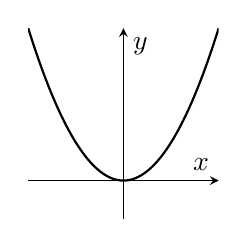
\begin{tikzpicture}[baseline={(current bounding box.center)}]
        \begin{axis}[
            width=4cm,
            height=4cm,
            axis x line=middle, axis y line=middle,
            xmin=-2, xmax=2, ymin=-1, ymax=4,
            ticks=none, xlabel=$x$, ylabel=$y$
        ]
        \addplot[domain=-2:2, samples=100, thick] {x^2};
        \end{axis}
    \end{tikzpicture} \\\\
    
    $\begin{array}{rl}
        \Psi:\, & [0,+\infty[\to\mathbb{R} \\
        x & \mapsto x^2
    \end{array}$ & Continua ma non uniformemente continua & 
    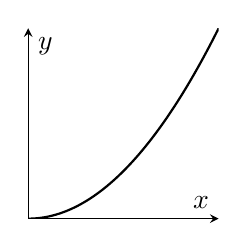
\begin{tikzpicture}[baseline={(current bounding box.center)}]
        \begin{axis}[
            width=4cm,
            height=4cm,
            axis x line=middle, axis y line=middle,
            xmin=0, xmax=2, ymin=0, ymax=4,
            ticks=none, xlabel=$x$, ylabel=$y$
        ]
        \addplot[domain=0:2, samples=100, thick] {x^2};
        \end{axis}
    \end{tikzpicture} \\\\
    
    $\begin{array}{rl}
        \varphi:\, & \mathbb{R}\setminus\{0\}\to\mathbb{R} \\
        x & \mapsto \frac{1}{x}
    \end{array}$ & Continua & 
    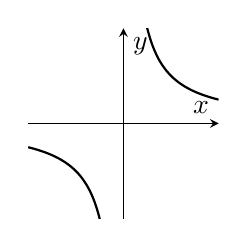
\begin{tikzpicture}[baseline={(current bounding box.center)}]
        \begin{axis}[
            width=4cm,
            height=4cm,
            axis x line=middle, axis y line=middle,
            xmin=-2, xmax=2, ymin=-2, ymax=2,
            ticks=none, xlabel=$x$, ylabel=$y$
        ]
        \addplot[domain=-2:-0.1, samples=100, thick] {1/x};
        \addplot[domain=0.1:2, samples=100, thick] {1/x};
        \end{axis}
    \end{tikzpicture} \\\\
    
    $\begin{array}{rl}
        \varphi:\, & ]0,1]\to\mathbb{R} \\
        x & \mapsto \frac{1}{x}
    \end{array}$ & Continua ma non uniformemente continua & 
    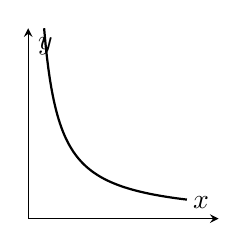
\begin{tikzpicture}[baseline={(current bounding box.center)}]
        \begin{axis}[
            width=4cm,
            height=4cm,
            axis x line=middle, axis y line=middle,
            xmin=0, xmax=1.2, ymin=0, ymax=10,
            ticks=none, xlabel=$x$, ylabel=$y$
        ]
        \addplot[domain=0.1:1, samples=100, thick] {1/x};
        \end{axis}
    \end{tikzpicture} \\
    
    \end{tabular}    
\end{table}

\vspace{10pt}

\paragraph{Continuità della funzione seno}
\begin{bxthm}
\begin{prop}
    La funzione seno è uniformemente continua.
\end{prop}
\end{bxthm}
\begin{proof}
    Sia $\varepsilon>0$ e prendiamo $\delta=\varepsilon$.
    $\forall\, x,w\in\mathbb{R}$ con $|x-w|<\delta$ dimostriamo che \(|\sin(x)-\sin(w)|<\varepsilon\).
    \begin{align*}
        |\sin(x)-\sin(w)|=&\, \left|2\sin\left(\dfrac{x-w}{2}\right)\cos\left(\dfrac{x+w}{2}\right)\right|= 2\left|\sin\left(\dfrac{x-w}{2}\right)\right|\cdot\left|\cos\left(\dfrac{x+w}{2}\right)\right|\\
                         \leq&\,  2\left|\sin\left(\dfrac{x-w}{2}\right)\right|\leq  2\left|\dfrac{x-w}{2}\right|=|x-w|<\delta=\varepsilon.
    \end{align*}
\end{proof}

\vspace{10pt}

\paragraph{Primo lemma del numero di Nepero}
\begin{bxthm}
\begin{lem}
    \[\forall\,t\in\mathbb{R},\quad |e^t-1|\leq e^{|t|}-1\]
\end{lem}
\end{bxthm}
\begin{proof}\hfill
    \begin{itemize}
        \item Se $t\geq0$, allora avremo rispettivamente
        \begin{itemize}
            \item $e^t\geq1\quad\implies\quad e^t-1\geq0 \quad\implies\quad |e^t-1|=e^t-1;$
            \item $|t|=t \quad\implies\quad e^{|t|}-1=e^t-1.$
        \end{itemize}
        da cui ricaviamo \[e^t-1=e^t-1.\]
        \item Se $t<0$ allora $e^t<1\implies e^t-1<0$ da cui 
        \[|e^t-1|=-(e^t-1)=1-e^t\]
        da $1=e^0=e^{t-t}$, procediamo con
        \[e^{t-t}-e^t=e^t(e^{-t}-1)<e^{-t}-1\]
        da $t<0$ abbiamo $|t|=-t$, per cui possiamo scrivere
        \[e^{|t|}-1=e^{-t}-1\]
        quindi \[|e^t-1|<e^{-t}-1=e^{|t|}-1\implies |e^t-1|<e^{|t|}-1.\]
    \end{itemize}
\end{proof}

\vspace{10pt}

\paragraph{Secondo lemma del numero di Nepero}
\begin{bxthm}
\begin{lem}
    \[\forall\,n\in\mathbb{N},\quad e^{\frac{1}{n}}-1\leq\dfrac{e-1}{n}.\]
\end{lem}
\end{bxthm}
\begin{proof}
    Sia $b=e^{\frac{1}{n}}-1$. Per la disuguaglianza di Bernoulli, 
    \[e=(1+b)^n\geq 1+nb=1+n(e^{\frac{1}{n}}-1).\]
    Dunque 
    \[e\geq 1+n(e^{\frac{1}{n}}-1)\]
    Ora, sottraendo $-1$ a entrambi i membri otteniamo
    \[e-1\geq n(e^{\frac{1}{n}}-1)\]
    dividendo entrambi i membri per $n$, abbiamo
    \[\dfrac{e-1}{n}\geq \dfrac{\cancel{n}(e^{\frac{1}{n}}-1)}{\cancel{n}}=(e^{\frac{1}{n}}-1).\]
    Da cui ricaviamo \[\frac{e-1}{n}\geq(e^{\frac{1}{n}}-1).\]
\end{proof}

\vspace{10pt}

\paragraph{Continuità della funzione esponenziale}
\begin{bxthm}
\begin{thm}
    La funzione esponenziale è continua.
\end{thm}
\end{bxthm}
\begin{proof}
    Sia $w\in\mathbb{R}$, allora $\forall\, \varepsilon >0$, prendiamo un $n\in\mathbb{N}$ maggiore di $\dfrac{e^w(e-1)}{\varepsilon}$ e sia $\delta=\dfrac{1}{n}\;(>0)$.
    Allora \[\forall\, x\in\mathbb{R}\,:\,|x-w|<\delta,\quad |e^x-e^w|\;=\;e^w|e^{x-w}-1|\;\leq\; e^w(e^{|x-w|}-1).\] 
    Da $|x-w|<\delta$, abbiamo che \[e^w(e^{|x-w|}-1)<e^w(e^\delta-1).\]
    Ciò implica 
    \[e^w(e^\delta-1)=e^w(e^{\frac{1}{n}}-1)\implies e^w(e^{\frac{1}{n}}-1)\leq\dfrac{e^w(e-1)}{n}<\varepsilon.\]
\end{proof}

\vspace{10pt}

\subsubsection{Continuità da destra e da sinistra}

\vspace{10pt}

\paragraph{Continuità da destra e da sinistra}
\begin{bxthm}
\begin{defn}
    Sia $f:A\to\mathbb{R}$ e sia $w\in A$.
    Diciamo che $f$ è \textbf{continua da sinistra} in $w$ se 
    \[\forall\, \varepsilon>0,\;\exists\,\delta>0\,:\,\forall\,x\in A\,\cap\,]w-\delta,w],\quad |f(x)-f(w)|<\varepsilon.\]
    Mentre diciamo che $f$ è \textbf{continua da destra} in $w$ se 
    \[\forall\, \varepsilon>0,\;\exists\,\delta>0\,:\,\forall\,x\in A\,\cap\,[w,w+\delta[,\quad |f(x)-f(w)|<\varepsilon.\]
\end{defn}
\end{bxthm}

\vspace{10pt}

\begin{exmp}
    La funzione di Dirichlet non è continua nè da destra nè da sinistra, mentre la funzione parte intera è sempre continua da destra mentre nei numeri interi non è continua da sinistra. 
\end{exmp}

\vspace{10pt}

\paragraph{Collegamento tra continuità e continuità da destra e da sinistra}
\begin{bxthm}
\begin{thm}
    Sia $f:A\to\mathbb{R}$ e sia $w\in A$. 
    Allora $f$ è continua in $w$ se e solo se lo è sia da destra sia da sinistra.
\end{thm}
\end{bxthm}
\begin{proof}
    Sia $f$ continua in $w$, fissiamo un $\varepsilon >0$.
    Per ipotesi 
    \[\exists\,\delta>0\,:\,\forall\, x\in A,\quad |x-w|<\delta\;\implies\; |f(x)-f(w)|<\varepsilon.\]
    Quindi sia per le $x\in A\,\cap\,]w-\delta,w] $, sia per le $x\in A\,\cap\, [w,w+\delta[$ si avrà \[|f(x)-f(w)|<\varepsilon.\]
    Viceversa, sia $f$ continua sia da destra sia da sinistra in $w$ e fissiamo $\varepsilon>0$, per la continuità da sinistra abbiamo che 
    \[\exists\,\delta'>0\,:\,\forall\, x\in A\,\cap\,]w-\delta',w] ,\quad |f(x)-f(w)|<\varepsilon.\]
    Per la continuità da destra, abbiamo invece che
    \[\exists\,\delta''>0\,:\,\forall\, x\in A\,\cap\, [w,w+\delta''[,\quad|f(x)-f(w)|<\varepsilon.\]
    Se dunque poniamo $\delta=\min\{\delta',\delta''\}$, allora avremo che 
    \[\forall\, x\in A\,\cap\, ]w-\delta,w+\delta[,\quad|f(x)-f(w)|<\varepsilon.\]
\end{proof}

\vspace{10pt}

\paragraph{Continuità delle funzioni monotòne}
\begin{bxthm}
\begin{prop}
    Siano $f:A\to\mathbb{R}$ monotòna e $w\in A$. Allora:\\
    \begin{enumerate}
        \item Se $f$ è crescente e \[\exists\,f(w)=\sup\{\,f(x)\,|\,x\in A\,\land\, x<w\,\},\] allora $f$ è \textbf{continua da sinistra} in $w$.\\
        \item Se $f$ è crescente e \[\exists\,f(w)=\inf\{\,f(x)\,|\,x\in A\,\land\, x>w\,\},\] allora $f$ è \textbf{continua da destra} in $w$.\\
        \item Se $f$ è decrescente e \[\exists\,f(w)=\inf\{\,f(x)\,|\,x\in A\,\land\, x<w\,\},\] allora $f$ è \textbf{continua da sinistra} in $w$.\\
        \item Se $f$ è decrescente e \[\exists\,f(w)=\sup\{\,f(x)\,|\,x\in A\,\land\, x>w\,\},\] allora $f$ è \textbf{continua da destra} in $w$.\\
    \end{enumerate}
\end{prop}
\end{bxthm}
\begin{proof}
    Considerando la (1), le altre sono analoghe.
    Sia dunque $f$ crescente e \[f(w)=\sup\{\,f(x)\,|\,x\in A\,\land\, x<w\,\}.\]
    Fissiamo $\varepsilon>0$.
    Per la caratterizzazione dell'estremo superiore esisterà $u\in A$, con $u<w$ tale che $f(u)>f(w)-\varepsilon$. 
    Poniamo $\delta=w-u(>0)$.
    Allora l'intervallo $A\,\cap\,]w-\delta,w]$ è riscrivibile come $A\,\cap\,]u,w]$.
    Abbiamo dunque che \[\forall\, x\in A\,\cap\,]u,w],\quad f(w)-\varepsilon<f(u)\leq f(x)\leq f(w)<f(w)+\varepsilon\] 
    e cioè che \[f(x)\in\,]f(w)-\varepsilon,f(w)+\varepsilon[\implies |f(x)-f(w)|<\varepsilon.\]
\end{proof}

\vspace{10pt}

\paragraph{Continuità in una certa restrizione a sinistra}
\begin{bxthm}
\begin{prop}
    La restrizione di $f$ a \(A^-_w=A\,\cap\,]-\infty,w],\) cioè la funzione \(f_{\upharpoonright \  A^-_w}(x),\) è continua da sinistra in $w$.
    Formalmente:
    \[\forall\,\varepsilon>0,\;\exists\,\delta>0\,:\,\forall\, x\in A^-_w\,\cap\,]w-\delta,w+\delta[,\;|f(x)-f(w)|<\varepsilon.\]
\end{prop}
\end{bxthm}
\begin{proof}
    Infatti 
    \[A^-_w\,\cap\,]w-\delta,w+\delta[\,=(A\,\cap\,]-\infty,w])\,\cap\,]w-\delta,w+\delta[=A\,\cap\,(\,]w-\delta,w+\delta[\,\cap\,]-\infty,w]\,)=A\,\cap\,]w-\delta,w].\]
    I due insiemi sono uguali e le due condizioni sono equivalenti.
\end{proof}

\vspace{10pt}

\begin{bxthm}
\begin{thm}
    Sia $f:A\to\mathbb{R}$ monotòna.
    Se $f(A)$ è un intervallo, allora $f$ è continua.
    (condizione sufficiente ma non necessaria).
\end{thm}
\end{bxthm}
\begin{proof}
    Prendiamo un qualunque $w\in A$ e dimostriamo che $f$ è continua da sinistra e da destra in $w$.
    Ci limitiamo alla continuità da sinistra (analogamente da destra).
    Supponiamo $f$ crescente.
    Se $w=\min A$ non c'è nulla da dimostrare perchè la funzione sarebbe automaticamente 
    continua da sinistra (lo sarebbe perchè la restrizione ad $A\,\cap\, ]-\infty,w]$ si ridurrebbe ad un singoletto).
    Altrimenti esiste almeno un $\nu\in A$ tale che $\nu<w$. 
    Poniamo \[s=\sup\{f(x)\,|\,x\in A\;\land\; x<w\},\]
    essendo la funzione crescente è $s\leq f(w)$ (dobbiamo dimostrare che $s=f(w)$).
    Supponiamo per assurdo $s<f(w)$ e sia $y\in\,]s,f(w)[$.
    \begin{itemize}
        \item \textbf{Caso 1: } $x\in A$ con $x<w\quad f(x)<s<y<f(w)$.
        \item \textbf{Caso 2: } $x\in A$ con $x\geq w\quad f(x)\geq f(w)>y$.
    \end{itemize}
    In ogni caso $y\notin f(A)$.
    D'altra parte, ricordiamo che c'è $\nu\in A$ con $\nu<w$, allora $f(\nu)\leq s<y<f(w)$, per cui 
    $y\in [f(\nu),f(w)[$ con $f(\nu),f(w)\in f(A)$. Quindi anche $y\in f(A)$, per cui si ha una contraddizione. 
    $y$ non può contemporaneamente appartenere e non appartenere a $f(A)$
\end{proof}

\vspace{10pt}

\paragraph{Continuità dell'inversa di una funzione strettamente monotòna}
\begin{bxthm}
\begin{cor}
    Sia $f:I\to\mathbb{R}$ strettamente monotòna con $I$ intervallo.
    Allora $f$ è invertibile e la sua inversa è continua.
\end{cor}
\end{bxthm}

\vspace{10pt}

\begin{note}
    Con ciò possiamo affermare che tutte le funzioni elementari sono continue nel loro dominio.
\end{note}

\vspace{10pt}

\subsubsection{Classificazione dei punti di discontinuità}

\vspace{10pt}

\paragraph{Discontinuità di prima e di seconda specie}
\begin{bxthm}
\begin{defn}
    Sia $f:A\to\mathbb{R}$ e $w\in A$.
    Se $f$ non è continua in $w$, diciamo che $w$ è un \textbf{punto di discontinuità} per $f$.
    Un punto di discontinuità $w\in A$ per una $f:A\to\mathbb{R}$ si dice di $1^\circ$ o $2^\circ$ specie, a seconda che valgano o no le seguenti condizioni:
    \begin{enumerate}
        \item $\exists\, f_-\,:\,A\to\mathbb{R}$, continua da sinistra in $w$ e tale che $\forall\, x\in A\setminus\{w\}$ si abbia $f_-(x)=f(x)$;
        \item $\exists\, f_+\,:\,A\to\mathbb{R}$, continua da destra in $w$ e tale che $\forall\, x\in A\setminus\{w\}$ si abbia $f_+(x)=f(x)$.
    \end{enumerate}
    Se entrambe queste condizioni sono soddisfatte, il punto di discontinuità è detto di prima specie. 
    Se almeno una di queste condizioni non è soddisfatta, il punto di discontinuità è detto di seconda specie.
\end{defn}
\end{bxthm}

\vspace{10pt}

\begin{exmp}
    La funzione segno definita con
    \[\textup{sgn}:\mathbb{R}\to\mathbb{R}\quad
        x\mapsto
        \begin{cases}
            -1\quad x<0\\
            0\quad x=0\\
            1\quad x>0
        \end{cases}\]
    \begin{center}
        \centering 
        \begin{tikzpicture}[scale=1]
            % Draw axes
            \draw[->] (-3,0) -- (3,0) node[right] {$x$};
            \draw[->] (0,-2) -- (0,2) node[above] {$y$};
            
            % Draw the function
            \draw[thick, blue] (-3,-1) -- (0,-1) node[below right] {$-1$};
            \draw[thick, blue] (0,1) -- (3,1) node[above right] {$1$};
            
            % Draw the points
            \fill[blue] (0,0) circle (2pt) node[below left] {$0$};
            \draw[blue] (0,0) circle (2pt);
            
            % Draw white dots to indicate undefined points
            \draw[fill=white, thick] (0,-1) circle (2pt);
            \draw[fill=white, thick] (0,1) circle (2pt);
            \draw[blue] (0,-1) circle (2pt);
            \draw[blue] (0,1) circle (2pt);
        
        \end{tikzpicture}
    \end{center}
    è una funzione che presenta una discontinuità di prima specie, la si può cioè rendere continua solo da destra o solo da sinistra)
\end{exmp}

\vspace{10pt}

\begin{exmp}
    La funzione definita con
    \[g:\mathbb{R}\to\mathbb{R}\quad 
        x\mapsto
        \begin{cases}
            \dfrac{1}{x}\quad x\neq0\\
            0\quad x=0
        \end{cases}\]
    \begin{center}
        \centering 
        \begin{tikzpicture}[scale=0.5]
            % Draw axes
            \draw[->] (-5,0) -- (5,0) node[right] {$x$};
            \draw[->] (0,-5) -- (0,5) node[above] {$y$};
            
            % Draw the function 1/x
            \draw[thick, blue, domain=-5:-0.2, samples=100] plot (\x,{1/\x});
            \draw[thick, blue, domain=0.2:5, samples=100] plot (\x,{1/\x});
            
            % Draw the point at (0,0)
            \draw[fill=blue, thick] (0,0) circle (2pt);
            \draw[blue] (0,0) circle (2pt);
        
        \end{tikzpicture}
    \end{center}
    è una funzione che presenta una discontinuità di seconda specie. Non si riesce a rettificarla per farla diventare continua nè da destra nè da sinistra
\end{exmp}

\vspace{10pt}

\begin{exmp}
    La funzione di Dirichlet è una funzione in cui non basta modificare il valore in un punto per farla diventare continua.
\end{exmp}


\vspace{10pt}

\paragraph{Discontinuità eliminabile}
\begin{bxthm}
\begin{defn}
    Una discontinuità di $1^\circ$ specie è \textbf{eliminabile} se $\exists\, f_\star:\mathbb{R}\to\mathbb{R}$ tale che (1) e (2) siano verificate ed inoltre
    $f_-=f_\star$ e $f_+=f_\star$ rispettivamente. 
    Quindi $f_\star$ è continua in $w$ e \[\forall\, x\in A\setminus\{w\},\quad f_\star(x)=f(x).\]    
\end{defn}
\end{bxthm}

\vspace{10pt}

\paragraph{Discontinuità di una funzione monotòna}
\begin{bxthm}
\begin{thm}
    Sia $f:A\to\mathbb{R}$ monotòna e discontinua in $w$. Allora tale discontinuità è di $1^\circ$ specie.
\end{thm}
\end{bxthm}

\vspace{10pt}

\subsection{Intorni}

\vspace{10pt}

\paragraph{Intorno e collezione di intorni di un punto}
\begin{bxthm}
\begin{defn}
    Sia $a\in\mathbb{R}$. Si chiama \textbf{intorno} di centro $a$ e raggio $\delta>0$, l'insieme 
    \[I_a(\delta)=\,]a-\delta,a+\delta[\,=\{x\in\mathbb{R} \,|\, |x-a|<\delta\}.\]
    L'insieme \[\mathcal{I}_a=\{I_a(\delta) \,|\, \delta>0\}\] è detto \textbf{collezione degli intorni di} $a$.
\end{defn}
\end{bxthm}

\vspace{10pt}

\paragraph{Intorno relativizzato}
\begin{bxthm}
\begin{defn}
    Siano $a\in A\subseteq\mathbb{R}$ e $I\in \mathcal{I}_a$. Diciamo che $I\cap A$ è un \textbf{intorno relativo} (o \textbf{relativizzato}).
\end{defn}
\end{bxthm}

\vspace{10pt}

\paragraph{Caratterizzazione della continuità mediante intorni}
\begin{note}
    Con queste definizioni si ha che una $f:A\to\mathbb{R}$ è continua in $w\in A$ se e solo se 
    \[\forall\, J\in \mathcal{I}_{f(w)},\;\exists\, I\in \mathcal{I}_w\,:\,f(I\cap A)\subseteq J.\]
\end{note}

\vspace{10pt}

\paragraph{Intorno destro e intorno sinistro}
\begin{bxthm}
\begin{defn}
    Siano $a\in\mathbb{R}$ e $\delta>0$, chiamiamo:
\begin{itemize}
    \item \textbf{Intorno destro} di $a$ l'intervallo 
    \[I^+_a(\delta)= \ ]a,a+\delta[\;;\]
    \item \textbf{Intorno sinistro} di $a$ l'intervallo 
    \[I^-_a(\delta)= \ ]a-\delta,a[\;.\]
\end{itemize}
Seguono rispettivamente i seguenti insiemi:
\begin{itemize}
    \item \textbf{Collezione degli intorni destri di $a$}.
    \[\mathcal{I}^+_{a}=\{I^+_a(\delta)\, |\, \delta>0\}\] 
    \item \textbf{Collezione degli intorni sinistri di $a$}.
    \[\mathcal{I}^-_{a}=\{I^-_a(\delta)\, |\, \delta>0\}\] 
\end{itemize}
\end{defn}
\end{bxthm}

\vspace{10pt}

\paragraph{Intorni infiniti}
\begin{bxthm}
\begin{defn}
    Sia $a\in\mathbb{R}$, chiamiamo:
    \begin{itemize}
        \item \textbf{Intorno di più infinito} un qualsiasi intervallo aperto illimitato superiormente:
        \[I_{+\infty}(a)= \ ]a , +\infty[ \ = \ \{x\in\mathbb{R} \,|\, x>a\}\;.\]
        \item \textbf{Intorno di meno infinito} un qualsiasi intervallo aperto illimitato inferiormente:
        \[I_{-\infty}(a)= \ ]-\infty , a[ \ = \ \{x\in\mathbb{R} \,|\, x<a\}\;;\]        
    \end{itemize}
    Avremo dunque rispettivamente i seguenti insiemi:
    \begin{itemize}
        \item \textbf{Collezione degli intorni di più infinito}.
        \[\mathcal{I}_{+\infty}=\{I_{+\infty}(a)\, |\, a\in\mathbb{R}\}\] 
        \item \textbf{Collezione degli intorni di meno infinito}.
        \[\mathcal{I}_{-\infty}=\{I_{-\infty}(a)\, |\, a\in\mathbb{R}\}\] 
    \end{itemize}  
    Dati $a,b\in\mathbb{R}$, con $a<b$, si definisce inoltre \textbf{intorno di infinito} l'unione tra un intorno di $-\infty$ e un intorno di $+\infty$, cioè:
    \[I_\infty(a,b)=I_{-\infty}(a)\cup I_{+\infty}(b)=\{x\in\mathbb{R}  \ | \ x<a\lor x>b\}\]
    Analogamente al caso di un punto reale $a$, possiamo parlare di \textbf{intorno circolare di infinito}: 
    \[I_\infty(a)= \ ]-\infty , -a[ \ \cup \ ]a , +\infty[\quad a\in\mathbb{R}.\]
\end{defn}
\end{bxthm}

\vspace{10pt}

\subsection{Teoremi importanti sulle funzioni}

\vspace{10pt}

\paragraph{Teorema della permanenza del segno}
\begin{bxthm}
\begin{thm}
    Sia $f:A\to\mathbb{R}$ continua in $w\in A$ con $f(w)>0$ ($f(w)<0$). Allora 
    \[\exists\, I\in \mathcal{I}_{w}\,:\,\forall\, x\in I\cap A,\quad f(x)>0\quad(f(x)<0).\]
\end{thm}
\end{bxthm}
\begin{proof}
    Sia $\varepsilon=f(w)>0$. Per la continuità abbiamo che 
    \[ \exists\, \delta>0 \,:\, f(I_w(\delta)\cap A)\subseteq I_{f(w)}(\varepsilon)=\,]f(w)-\varepsilon,f(w)+\varepsilon[\,=\,]0,2f(w)[. \]
    Quindi 
    \[\forall\, x\in I_w(\delta)\cap A,\quad f(x)\in \,]\,0\,,\,2f(w)\,[\quad\therefore\quad f(x)>0.\]
\end{proof}

\vspace{10pt}

\paragraph{Teorema di esistenza degli zeri}
\begin{bxthm}
\begin{thm}
    Sia $f:[a,b]\to\mathbb{R}$ continua il cui dominio è un intervallo chiuso e limitato.
    Se $f(a)<0$ e $f(b)>0$, allora \[\exists\, c\in \,]a,b[\;:\,f(c)=0.\]
\end{thm}
\end{bxthm}
\begin{proof}
    Sia \[E=\{x\in[a,b]\, |\, f(x)<0\}\] poichè $a\in E$ si ha $E\neq\emptyset$.
    Inoltre $E\subseteq[a,b]$ ed è perciò un insieme limitato, e quindi ponendo $\sup(E)=s\in[a,b]$, avremo $a\leq s\leq b$.
    Dimostriamo che non si può avere $f(s)<0$, nè $f(s)>0$ e perciò avremo $f(s)=0$.
    \begin{itemize}
        \item Se $f(s)<0$, anzitutto $s<b$ (perchè $f(b)>0$).\\
        Per il teorema di permanenza del segno \[\exists\, \delta>0 \,:\, \forall\, x\in\, ]s-\delta,s+\delta[\,\cap\,[a,b],\quad f(x)<0.\] 
        Sia ora \[y=\min\left\{s+\dfrac{\delta}{2},b\right\},\] allora $y>s$ e $[s,y]$ è un intervallo. 
        Abbiamo dunque che 
        \[\forall\, x\in\,[s,y],\,x\in\, ]s-\delta,s+\delta[\,\cap\,[a,b]\]
        per cui $f(x)<0$.
        Da ciò segue $f(y)<0$, il che è assurdo poichè $y\notin E$ essendo $y$ maggiore dell'estremo superiore di $E$.

        \item Se $f(s)>0$, anzitutto $s>a$ (perchè $f(a)<0$).\\
        Per il teorema di permanenza del segno, 
        \[\exists\,\delta>0\,:\,\forall\, x\in\, ]s-\delta,s+\delta[\,\cap\,[a,b],\quad f(x)>0.\]
        Sia \[z=\max\left\{s-\dfrac{\delta}{2},a\right\},\] allora $z<s$ e $[z,s]$ è un intervallo. 
        Abbiamo dunque che 
        \[\forall\, x\in\,[z,s],\,x\in\, ]s-\delta,s+\delta[\,\cap\,[a,b]\]
        per cui $f(x)>0$. Da cui $f(z)>0$, per cui $z\notin E$, così come non appartengono ad $E$ tutte le $x\in[z,s]$.
        Dunque $E\subseteq[a,z]$ e $\sup E\leq z$, il che è assurdo perchè $\sup E=s>z.$
    \end{itemize}
\end{proof}

\vspace{10pt}

\paragraph{Teorema dei valori intermedi}
\begin{bxthm}
\begin{thm}
    Sia $I\subseteq\mathbb{R}$ un intervallo. Se $f:I\to\mathbb{R}$ è continua, anche $f(I)$ è un intervallo (eventualmente degenere).
    Equivalentemente, $\forall\,\alpha,\beta\in f(I)$ con $\alpha<\beta$ e $\forall\,y\in\,]\alpha,\beta[,\;y\in f(I)$.
    Cioè \[\exists\, x\in I: f(x)=y.\]
\end{thm}
\end{bxthm}
\begin{proof}
    Siano $\alpha,\beta\in f(I)$ con $\alpha<\beta$, e possiamo prendere $a,b\in I$ tali che $f(a)=\alpha$ e $f(b)=\beta$.
    Possiamo supporre che $a<b$ (ovvero $a\neq b$).
    Sia ora $y\in\,]\alpha,\beta[$, diciamo che \[\exists\, c\in\,]a,b[\,\subseteq I\,:\,f(c)=y.\]
    Sia 
    \begin{align*}
        g:I&\to\mathbb{R}\\
        x&\mapsto f(x)-y
    \end{align*}
    avremo allora
    \begin{align*}
        g(a)=&\,f(a)-y=\alpha-y<0\\
        g(b)=&\,f(b)-y=\beta-y>0\\
    \end{align*}
    Per il teorema degli zeri, \[\exists\, c\in\, ]a,b[\,:\,g(c)=0\] ossia $f(c)=y$.
\end{proof}

\vspace{10pt}

\paragraph{Caratterizzazione delle funzioni continue invertibili}
\begin{bxthm}
\begin{prop}
    Sia $f:I\to\mathbb{R}$ continua con $I$ intervallo. Allora $f$ è invertibile se e solo se è strettamente monotòna.
\end{prop}
\end{bxthm}
\begin{proof}
    Sia $f$ invertibile, e supponiamo non strettamente monotòna, allora abbiamo che 
    \[\exists\, p,q,r\in I\;(p<q<r)\;:\,f(q)\notin\,]f(p),f(r)[,\]
    quindi
    \[f(q)<\min\{f(p),f(r)\}\quad\lor\quad f(q)>\max\{f(p),f(r)\}.\]
    Se $f(q)<f(p)$, allora $f(p)\in\, ]f(q),f(r)[$.
    Per il teorema dei valori intermedi applicato a $f\in[q,r]$ troviamo \[c\in\,]q,r[\,:\,f(c)=f(p).\]
    Ma $c\neq p$, dunque è assurdo.
\end{proof}

\vspace{10pt}

\paragraph{Continuità dell'inversa di una funzione continua}
\begin{bxthm}
\begin{cor}
    Se $f:I\to\mathbb{R}$ è continua e invertibile con $I$ intervallo, anche l'inversa di $f$ è continua.
\end{cor}
\end{bxthm}
\begin{proof}
    Infatti $f$ è strettamente monotòna per la proposizione precedente.
\end{proof}

\vspace{10pt}

\paragraph{Criterio di continuità per le funzioni monotòne}
\begin{bxthm}
\begin{thm}
    Sia $f:I\to\mathbb{R}$ monotòna con $I$ intervallo. Allora 
    \[f\textup{ è continua}\quad\iff\quad f(I) \textup{ è un intervallo}.\]
\end{thm}
\end{bxthm}

\vspace{10pt}

\subsection{Punti isolati, punti esterni e punti di accumulazione}

\vspace{10pt}

\paragraph{Punti isolati, punti esterni e punti di accumulazione}
\begin{bxthm}
\begin{defn}
    Siano $A\subseteq\mathbb{R}$ e $p\in\mathbb{R}$. Diciamo che:
    \begin{itemize}
        \item $p$ è un punto \textbf{isolato} di $A$ se ($p\in A$)
        \[\exists\, I\in \mathcal{I}_p\,:\,I\cap A=\{p\};\]
        \item $p$ è un punto \textbf{esterno} di $A$ se ($p\notin A$)
        \[\exists\, I\in \mathcal{I}_p\,:\, I\cap A=\emptyset;\]
        \item $p$ è un punto \textbf{di accumulazione} per $A$ se 
        \[\forall\, I\in \mathcal{I}_p,\, I\cap A\setminus\{p\}\neq\emptyset.\]
        L'insieme dei punti di accumulazione si indica con 
        \[\mathcal{D}(A)=\{\,p\in\mathbb{R} \ | \ p \textup{ è di accumulazione per }A\,\}.\]
    \end{itemize}
\end{defn}
\end{bxthm}

\vspace{10pt}

\begin{note}
    Dalla definizione segue subito 
    \[p\in\mathcal{D}(A)\;\iff\; p\in\mathcal{D}(A\setminus\{p\})\;\iff\; p\in\mathcal{D}(A\cup\{p\}).\] 
    Cioè che $p$ può appartenere o no ad $A$.
\end{note}

\vspace{10pt}

\begin{exmp}
    \begin{enumerate}\hfill
        \item \[p\in A,\quad p\in\mathcal{D}(A),\quad p=0,\quad A=[0,1]\] (in generale, se $A$ intervallo non degenere).
        \item \[p\in A,\quad p\notin\mathcal{D}(A),\quad p=0,\quad A=\{0\}\] (anche se $A\subseteq\mathbb{Z}$ e $p\in A$).
        \item \[p\notin A,\quad p\in\mathcal{D}(A),\quad p=0,\quad A=]0,1]\] anche $A=\mathbb{R}\setminus \mathbb{Q}$, $p\in\mathbb{Q}$ viceversa, $A=\mathbb{Q}$, $p\in\mathbb{Q}$.
        \item \[p\notin A,\quad p\notin\mathcal{D}(A),\quad p=0,\quad A=\emptyset\;\lor\; A=[1,+\infty[.\]
        \item Se $p\notin\mathcal{D}(A)$, allora $p$ è isolato in $A$ se $p\in A$ ed esterno in $A$ se $p\notin A$.
    \end{enumerate}
\end{exmp}

\vspace{10pt}

\paragraph{Continuità in un punto isolato}
\begin{bxthm}
\begin{prop}
    Siano $f:A\to\mathbb{R}$ e $p$ un punto isolato. Allora $f$ è continua in $p$.
\end{prop}
\end{bxthm}
\begin{proof}
    Per ipotesi \[\exists\,\delta>0\,:\,I_p(\delta)\cap A=\{p\}.\]
    Sia $\varepsilon>0$, allora \[\forall\, x\in I_p(\delta)\cap A,\quad x=p,\] quindi \[|f(x)-f(p)|=0<\varepsilon.\]
\end{proof}

\vspace{10pt}

\paragraph{Collegamento tra punti di discontinuità e punti di accumulazione}
\begin{bxthm}
\begin{cor}\label{coroo}
    Sia $p\in A$ punto di discontinuità per $f:A\to\mathbb{R}$. Allora $p$ è punto di accumulazione per $A$.
\end{cor}
\end{bxthm}

\vspace{10pt}

\begin{bxthm}
\begin{prop}
    Siano $w\in A$ e 
    \[ f:A\to\mathbb{R}\quad
        x\mapsto\begin{cases}
            0 \quad\,\quad\quad x\neq w\\
            y\neq0 \quad\; x=w
        \end{cases}. \]
    Allora $\forall\, y\neq0, \;f$ è discontinua in $w$ se e solo se $w\in\mathcal{D}(A)$.
\end{prop}
\end{bxthm}
\begin{proof}\hfill
    \begin{itemize}
        \item[$\implies$]
        Se $f$ è discontinua, allora $w\in\mathcal{D}(A)$ per il corollario (\ref{coroo}).
        \item[$\impliedby$]
        Viceversa, se $f$ fosse continua allora per il teorema di permanenza del segno, 
        \[\exists\, I\in \mathcal{I}_w\, :\, \forall\, x\in A\cap I,\quad f(x)\neq0.\]
        Quindi $A\cap I=\{w\}$. Pertanto $w$ è isolato in $A$, per cui $w\notin\mathcal{D}(A)$.
    \end{itemize}
\end{proof}

\vspace{50pt}
\part{Limiti e Successioni}
\vspace{50pt}

\section{Limiti}
\vspace{50pt}

\paragraph{Limiti fondamentali delle funzioni elementari}
\begin{multicols}{2}
\begin{itemize}
    \item[] \[\lim\limits_{x\to\infty}c=c\]
    \item[] \[\lim\limits_{x\to\pm\infty}x=\pm\infty\]
    \item[] \[\lim\limits_{x\to\infty}\frac{1}{x}=0\]
    \item[] \[\lim\limits_{x\to 0^-}\frac{1}{x}=-\infty\quad \lim\limits_{x\to0^+}\frac{1}{x}=+\infty\]
    \columnbreak
    \item[] \[\lim\limits_{x\to -\infty}e^x=0\quad \lim\limits_{x\to +\infty}e^x=+\infty\]
    \item[] \[\lim\limits_{x\to (\frac{\pi}{2})^-}\tan x=-\infty\quad \lim\limits_{x\to (\frac{\pi}{2})^+}\tan x=+\infty\]
    \item[] \[\lim\limits_{x\to -\infty}\arctan x=-\frac{\pi}{2}\quad \lim\limits_{x\to+\infty}\arctan x=\frac{\pi}{2}\]
    \item[] \[\lim\limits_{x\to 0}\log x=-\infty\quad \lim\limits_{x\to+\infty}\log x=+\infty\]
\end{itemize}
\end{multicols}

\vspace{10pt}

\paragraph{Limiti notevoli}
\subparagraph{Limiti notevoli di funzioni esponenziali e logaritmiche}
\begin{multicols}{2}
\begin{enumerate}
    \item[] \textbf{Logaritmo Naturale}
    \[\lim_{x\to0}\dfrac{\ln(1+x)}{x}=\lim_{f(x)\to0}\dfrac{\ln(1+f(x))}{f(x)}=1\]
    \[\lim_{x\to0}\dfrac{x}{\ln(1+x)}=\lim_{f(x)\to0}\dfrac{f(x)}{\ln(1+f(x))}=1\]
    \[\lim_{x\to0}\dfrac{\ln(1+nx)}{mx}=\lim_{f(x)\to0}\dfrac{\ln(1+nf(x))}{mf(x)}=\dfrac{n}{m}\]
    \[\lim_{x\to0}\dfrac{mx}{\ln(1+nx)}=\lim_{f(x)\to0}\dfrac{mf(x)}{\ln(1+nf(x))}=\dfrac{m}{n}\]
    \[\lim_{x\to0}\dfrac{\ln(1+ax)}{\ln(1+bx)}=\dfrac{a}{b}\]
    \[\lim_{x\to0}\dfrac{\ln x-\ln a}{x-a}=\lim_{f(x)\to0}\dfrac{\ln f(x)-\ln a}{f(x)-a}=\dfrac{1}{a}\]
    \[\lim_{x\to0}\dfrac{x-a}{\ln x-\ln a}=\lim_{f(x)\to0}\dfrac{f(x)-a}{\ln f(x)-\ln a}=a\]
    \item[] \textbf{Logaritmo}
    \[\lim_{x\to0}\dfrac{\log_a(1+x)}{x}=\lim_{f(x)\to0}\dfrac{\log_a(1+f(x))}{f(x)}=\dfrac{1}{\ln(a)}\]
    \[\lim_{x\to0}\dfrac{x}{\log_a(1+x)}=\lim_{f(x)\to0}\dfrac{f(x)}{\log_a(1+f(x))}=\ln(a)\]
    \item[] \textbf{Potenza}
    \[\lim_{x\to1}\dfrac{x^\alpha-1}{x-1}=\alpha\]
    \[\lim_{x\to+\infty}\dfrac{x^n+a}{x^n}^{bx^n}=ab\] 
    \item[] \textbf{Esponenziale Naturale}
    \[\lim_{x\to0}\dfrac{e^x-1}{x}=\lim_{f(x)\to0}\dfrac{e^{f(x)}-1}{f(x)}=1\]
    \[\lim_{x\to0}\dfrac{x}{e^x-1}=\lim_{f(x)\to0}\dfrac{f(x)}{e^{f(x)}-1}=1\]
    \[\lim_{x\to0}\dfrac{e^{ax}-1}{bx}=\lim_{f(x)\to0}\dfrac{e^{af(x)}-1}{bf(x)}=\dfrac{a}{b}\]
    \[\lim_{x\to0}\dfrac{bx}{e^{ax}-1}=\lim_{f(x)\to0}\dfrac{bf(x)}{e^{af(x)}-1}=\dfrac{b}{a}\]
    \item[] \textbf{Esponenziale con Base Arbitraria}
    \[\lim_{x\to0}\dfrac{a^x-1}{x}=\lim_{f(x)\to0}\dfrac{a^{f(x)}-1}{f(x)}=\ln(a)\]
    \[\lim_{x\to0}\dfrac{x}{a^x-1}=\lim_{f(x)\to0}\dfrac{f(x)}{a^{f(x)}-1}=\dfrac{1}{\ln(a)}\]
    \[\lim_{x\to0}\dfrac{a^{mx}-1}{nx}=\lim_{f(x)\to0}\dfrac{a^{mf(x)}-1}{nf(x)}=\dfrac{m\ln(a)}{n}\]
    \[\lim_{x\to0}\dfrac{nx}{a^{mx}-1}=\lim_{f(x)\to0}\dfrac{nf(x)}{a^{mf(x)}-1}=\dfrac{n}{m\ln(a)}\]
    \[\lim_{x\to0}\dfrac{a^x-1}{x-1}=a^x\ln(a)\]
    \item[] \textbf{Numero di Nepero}
    \[\lim_{x\to\infty}\left(1+\dfrac{1}{x}\right)^x=\lim_{f(x)\to\infty}\left(1+\dfrac{1}{f(x)}\right)^{f(x)}=e\]
    \[\lim_{x\to\infty}\left(1+\dfrac{1}{x}\right)^x=\lim_{x\to\infty}\left(1+\dfrac{1}{x+a}\right)^x\quad a\in\mathbb{R}\]
    \[\lim_{x\to\infty}\left(1+\dfrac{k}{x}\right)^{nx}=e^{kn}\] 
    \[\lim_{x\to a}\dfrac{e^x-e^a}{x-a}=e^a\]
    \[\lim_{x\to\infty}(1+x)^{\dfrac{1}{x}}=e\]
    \[\lim_{x\to\infty}(1+cx^n)^{\dfrac{k}{cx^n}}=e^{kc}\]
    \item[] \textbf{Potenza con Differenza}
    \[\lim_{x\to0}\dfrac{(1+x)^c-1}{x}=\lim_{f(x)\to0}\dfrac{(1+f(x))^c-1}{f(x)}=c\]
\end{enumerate}
\end{multicols}

\vspace{10pt}

\paragraph{Limiti Notevoli di Funzioni Trigonometriche}
\begin{multicols}{2}
\begin{enumerate}
    \item[] \textbf{Seno}
    \[\lim_{x\to0}\dfrac{\sin x}{x}=\lim_{f(x)\to0}\dfrac{\sin f(x)}{f(x)}=1\]
    \[\lim_{x\to0}\dfrac{\sin^n x}{\sin x^n}=\lim_{f(x)\to0}\dfrac{\sin^n f(x)}{\sin f^n(x)}=1\]
    \[\lim_{x\to0}\dfrac{\sin x^n}{\sin^n x}=\lim_{f(x)\to0}\dfrac{\sin f^n(x)}{\sin^n f(x)}=1\]
    \[\lim_{x\to0}\dfrac{\sin nx}{mx}=\dfrac{n}{m}\quad\lim_{x\to0}\dfrac{mx}{\sin nx}=\dfrac{m}{n}\] 
    \item[] \textbf{Coseno}
    \[\lim_{x\to0}\dfrac{1-\cos x}{x^2}=\lim_{f(x)\to0}\dfrac{1-\cos f(x)}{f^2(x)}=\dfrac{1}{2}\]
    \[\lim_{x\to0}\dfrac{1-\cos x}{x}=\lim_{f(x)\to0}\dfrac{1-\cos f(x)}{f(x)}=0\]
    \item[] \textbf{Tangente}
    \[\lim_{x\to0}\dfrac{\tan x}{x}=\lim_{f(x)\to0}\dfrac{\tan f(x)}{f(x)}=1\]
    \[\lim_{x\to0}\dfrac{x}{\tan x}=\lim_{f(x)\to0}\dfrac{f(x)}{\tan f(x)}=1\]
    \[\lim_{x\to0}\dfrac{\tan^n x}{x^n}=\lim_{x\to0}\dfrac{x^n}{\tan^n x}=1\]
    \[\lim_{x\to0}\dfrac{\tan mx}{nx}=\dfrac{m}{n}\] 
    \[\lim_{x\to0}\dfrac{nx}{\tan mx}=\dfrac{n}{m}\] 
    \item[] \textbf{Arcoseno}
    \[\lim_{x\to0}\frac{\arcsin x}{x}=\lim_{f(x)\to0}\frac{\arcsin f(x)}{f(x)}=1\]
    \[\lim_{x\to0}\frac{x}{\arcsin x}=\lim_{f(x)\to0}\frac{f(x)}{\arcsin f(x)}=1\]
    \item[] \textbf{Arcocoseno}
    \[\lim_{x\to0}\frac{\arccos^2(1-x)}{x}=2\]
    \item[] \textbf{Arcotangente}
    \[\lim_{x\to0}\frac{\arctan x}{x}=\lim_{f(x)\to0}\frac{\arctan f(x)}{f(x)}=1\]
    \[\lim_{x\to0}\frac{x}{\arctan x}=\lim_{f(x)\to0}\frac{f(x)}{\arctan f(x)}=1\]
\end{enumerate}
\end{multicols}

\vspace{50pt}

\subsection{Limite finito per $x$ che tende a $p$}

\vspace{10pt}

\paragraph{Limite finito per $x$ che tende a $p$}
\begin{bxthm}
\begin{defn}
    Siano $f:A\to\mathbb{R}$ e $p\in\mathcal{D}(A)$.
    Diciamo che $l\in\mathbb{R}$ è \textbf{limite} di $f$ in $p$ se
    \[\forall\,\varepsilon>0,\;\exists\,\delta>0\,:\,\forall\, x\in A\cap I_p(\delta)\setminus\{p\},\quad |\,f(x)-l\,|<\varepsilon\]
    equivalentemente 
    \[\forall\, J\in \mathcal{I}_l,\;\exists\, I\in \mathcal{I}_p\,:\,f(A\cap I\setminus\{p\})\subseteq J.\]
    Se $l$ esiste è unico e scriveremo 
    \[l=\lim_{x\to p} f(x).\]
\end{defn}
\end{bxthm}

\vspace{10pt}

\paragraph{Collegamento tra continuità e limiti di funzioni}
\begin{bxthm}
\begin{prop}
    Se $p\in\mathcal{D}(A)$ allora 
    \[f:A\to\mathbb{R}\;\textup{ è continua in }p\quad\iff\quad \lim_{x\to p} f(x)=f(p).\]
\end{prop}
\end{bxthm}

\vspace{20pt}

\subsection{Limite infinito per $x$ che tende a $p$}

\vspace{10pt}

\paragraph{Limite $+\infty$ per $x$ che tende a $p$}
\begin{bxthm}
\begin{defn}
    Siano $f:A\to\mathbb{R}$ e $p\in\mathcal{D}(A)$.
    Diciamo che $+\infty$ è limite di $f$ in $p$ se:
    \[\forall\, M>0,\;\exists\,I\in\mathcal{I}_{p}\;:\,\forall\, x\in A\cap I\setminus\{p\},\quad f(x)>M.\]
    Scriveremo 
    \[\lim_{x\to p}f(x)=+\infty.\]
\end{defn}
\end{bxthm}
\begin{note}
    Si dice anche che la funzione $f$ \textbf{diverge positivamente}.
\end{note}

\vspace{10pt}

\paragraph{Limite $-\infty$ per $x$ che tende a $p$}
\begin{bxthm}
\begin{defn}
    Siano $f:A\to\mathbb{R}$ e $p\in\mathcal{D}(A)$.
    Diciamo che $-\infty$ è limite di $f$ in $p$ se:
    \[\forall\, M>0,\;\exists\,I\in\mathcal{I}_{p}\;:\,\forall\, x\in A\cap I\setminus\{p\},\quad f(x)<-M.\]
    Scriveremo:
    \[\lim_{x\to p}f(x)=-\infty.\] 
\end{defn}
\end{bxthm}
\begin{note}
    Si dice anche che la funzione $f$ \textbf{diverge negativamente}.
\end{note}

\vspace{10pt}

\paragraph{I limiti destro e sinistro infiniti}
\begin{note}
    Anche per i limiti infiniti si possono distinguere limiti destri e limiti sinistri:
\begin{itemize}
    \item $\lim\limits_{x\to p^+}f(x)=+\infty$
    \[\forall\, M>0,\;\exists\,I\in\mathcal{I}^+_{p}\;:\,\forall\, x\in A\cap I\setminus\{p\},\quad f(x)>M;\]
    \item $\lim\limits_{x\to p^-}f(x)=+\infty$
    \[\forall\, M>0,\;\exists\,I\in\mathcal{I}^-_{p}\;:\,\forall\, x\in A\cap I\setminus\{p\},\quad f(x)>M;\]
    \item $\lim\limits_{x\to p^+}f(x)=-\infty$
    \[\forall\, M>0,\;\exists\,I\in\mathcal{I}^+_{p}\;:\,\forall\, x\in A\cap I\setminus\{p\},\quad f(x)<-M;\]
    \item $\lim\limits_{x\to p^-}f(x)=-\infty$
    \[\forall\, M>0,\;\exists\,I\in\mathcal{I}^-_{p}\;:\,\forall\, x\in A\cap I\setminus\{p\},\quad f(x)<-M.\]
\end{itemize}
\end{note}

\vspace{20pt}

\subsection{Limite finito di una funzione per $x$ che tende a infinito}

\vspace{10pt}

\paragraph{Limite finito di una funzione per $x$ che tende a $\infty$}
\begin{bxthm}
\begin{defn}
    Sia $f:A\to\mathbb{R}$. Diciamo che 
    \begin{itemize}
        \item $l\in\mathbb{R}$ è limite di $f$ in $+\infty$, e scriviamo $\lim\limits_{x\to+\infty}f(x)=l$, se 
        \[\forall\,\varepsilon>0,\;\exists\, M>0\,:\;\forall\, x>M,\quad |f(x)-l|<\varepsilon;\]
        \item $l\in\mathbb{R}$ è limite di $f$ in $-\infty$, e scriviamo $\lim\limits_{x\to-\infty}f(x)=l$, se 
        \[\forall\,\varepsilon>0,\;\exists\, M>0\,:\;\forall\, x<-M,\quad |f(x)-l|<\varepsilon.\]
    \end{itemize}
\end{defn}
\end{bxthm}

\vspace{20pt}

\subsection{Limite infinito di una funzione per $x$ che tende a infinito}

\vspace{10pt}

\paragraph{Limite $\infty$ di una funzione per $x$ che tende a $\infty$}
\begin{bxthm}
\begin{defn}
    Sia $f:A\to\mathbb{R}$. Diciamo che 
    \begin{itemize}
        \item $+\infty$ è il limite di $f$ in $+\infty$, e scriviamo $\lim\limits_{x\to+\infty}f(x)=+\infty$, se 
        \[\forall\,M>0,\;\exists\,c>0\,:\;\forall\,x>c,\;f(x)>M;\]
        \item $+\infty$ è il limite di $f$ in $-\infty$, e scriviamo $\lim\limits_{x\to-\infty}f(x)=+\infty$, se 
        \[\forall\,M>0,\;\exists\,c>0\,:\;\forall\,x<-c,\;f(x)>M;\]
        \item $-\infty$ è il limite di $f$ in $+\infty$, e scriviamo $\lim\limits_{x\to+\infty}f(x)=-\infty$, se 
        \[\forall\,M>0,\;\exists\,c>0\,:\;\forall\,x>c,\;f(x)<-M;\]
        \item $-\infty$ è il limite di $f$ in $-\infty$, e scriviamo $\lim\limits_{x\to-\infty}f(x)=-\infty$, se 
        \[\forall\,M>0,\;\exists\,c>0\,:\;\forall\,x<-,\;f(x)<-M;\]
    \end{itemize}
\end{defn}
\end{bxthm}

\vspace{10pt}

\subsection{Punti di accumulazione in senso lato}

\vspace{10pt}

\begin{bxthm}
\begin{defn}
    Siano $p\in\overline{\mathbb{R}}$ e $A\subseteq\mathbb{R}$.
    Diciamo che $p$ è \textbf{punto di accumulazione in senso lato} per $A$ e scriviamo 
    $p\in\overline{\mathcal{D}}(A)$ se 
    \[\forall\, I\in \mathcal{I}_p,\quad A\cap I\setminus\{p\}\neq\emptyset.\]
\end{defn}
\end{bxthm}

\vspace{10pt}

\begin{note}
    In particolare :
    \[+\infty\in\overline{\mathcal{D}}(A)\iff A\textup{ è illimitato superiormente, e }\;-\infty\in\overline{\mathcal{D}}(A)\iff A\textup{ è illimitato inferiormente}.\]
\end{note}

\vspace{10pt}

\begin{bxthm}
\begin{prop}
    Siano $p,q$ punti distinti di $\overline{\mathbb{R}}$, allora
    \[\exists\,I\in \mathcal{I}_p,\,J\in \mathcal{I}_q\;:\; I\cap J=\emptyset.\]
\end{prop}
\end{bxthm}
\begin{proof}
    Possiamo supporre $p<q$.
    \begin{enumerate}
        \item[] $p=-\infty,\; q\in\mathbb{R}$ \\
        Prendiamo $\varepsilon>0$ e sia $k>0$ con $k>-q+\varepsilon$, così $-k<q-\varepsilon$.
        Quindi gli intorni 
        \[I=\,]-\infty,-k[\quad\textup{e}\quad J=\,]q-\varepsilon,q+\varepsilon[\] 
        sono disgiunti.\\
        \item[] $p=-\infty,\; q=+\infty$ \\
        \[\forall\, k>0,\;\forall\, M>0,\quad I=\,]-\infty,-k[\quad\textup{e}\quad J=]M,+\infty[\] 
        sono disgiunti.\\
        \item[] $p\in\mathbb{R},\; q\in\mathbb{R}$ \\
        Poniamo \[\varepsilon=\dfrac{q-p}{2}>0,\] allora \[p+\varepsilon=q-\varepsilon=\frac{p+q}{2}.\]
        Gli intorni 
        \[I=\,]p-\varepsilon,p+\varepsilon[\quad\textup{e}\quad J=\,]q-\varepsilon,q+\varepsilon[.\]
        sono disgiunti.\\
        \item[] $p\in\mathbb{R},\; q=+\infty$ \\
        Prendiamo $\varepsilon>0$ e $k>0$ con $k>p+\varepsilon$. Gli intorni 
        \[I=\,]p-\varepsilon,p+\varepsilon[\quad\textup{e}\quad J=\,]k,+\infty[\]
        sono disgiunti.
    \end{enumerate}
\end{proof}

\vspace{10pt}

\subsection{Unicità del limite}

\vspace{10pt}

\paragraph{Unicità del limite}
\begin{bxthm}
\begin{cor}
    Il limite di una funzione $f:A\to\mathbb{R}$ in un punto $p\in\overline{\mathcal{D}}(A)$, se esiste è unico.
\end{cor}
\end{bxthm}
\begin{proof}
    Supponiamo per assurdo che $l',l''$ siano entrambi limiti di $f$ in $p$ con $l'\neq l''$.
    Per la proprietà precedente abbiamo che 
    \[\exists\,J'\in \mathcal{I}_{l'},\,J''\in \mathcal{I}_{l''}\;:\;J'\cap J''=\emptyset.\]
    Per la definizione di limite, abbiamo che
    \[\exists\,I',\,I''\in \mathcal{I}_p\,:\,f(I'\cap A\setminus\{p\})\subseteq J' \quad\land\quad f(I''\cap A\setminus\{p\})\subseteq J''.\]
    Sia ora $I=I'\cap I''\in \mathcal{I}_p$, si ha che 
    \[f(I\cap A\setminus\{p\})\subseteq f(I'\cap A\setminus\{p\})  \quad\land\quad f(I\cap A\setminus\{p\})\subseteq f(I''\cap A\setminus\{p\}),\]  
    cioè 
    \[f(I\cap A\setminus\{p\})\subseteq J'\cap J''=\emptyset.\]
    da cui $I\cap A\setminus\{p\}=\emptyset$, il che è impossibile con l'ipotesi che sia $p$ punto di accumulazione.
\end{proof}

\vspace{10pt}

\subsection{Operazioni con i limiti}

\vspace{10pt}

\paragraph{Operazioni con i limiti}
\begin{bxthm}
\begin{thm}
    Siano $f,g:A\to\mathbb{R}$ e $p\in\overline{\mathcal{D}}(A)$ e supponiamo che esistano
    \[\lim_{x\to p} f(x)=l\quad\textup{e}\quad\lim_{x\to p}g(x)=m.\]
    Allora 
    \begin{enumerate}
        \item $\lim\limits_{x\to p}(f+g)(x)=l+m$ eccetto il caso in cui $l=-\infty$ e $m=+\infty$ (o viceversa);
        \item $\lim\limits_{x\to p}(f\cdot g)(x)=l\cdot m$ eccetto il caso in cui $l=\pm\infty$ e $m=0$ (o viceversa).
    \end{enumerate}
\end{thm}
\end{bxthm}

\vspace{10pt}

\subsection{Limite della composizione di due funzioni}

\vspace{10pt}

\paragraph{Primo teorema sul limite della composizione}
\begin{bxthm}
\begin{thm}
    Siano 
    \[f:A\to B\textup{ con }p\in\overline{\mathcal{D}}(A)\;\textup{ e }\;g:B\to\mathbb{R}\textup{ con }q\in\overline{\mathcal{D}}(B).\]
    Supponiamo che 
    \[\lim_{x\to p}f(x)=q\quad\textup{ e che }\quad\lim_{y\to q}g(y)=l\in\overline{\mathbb{R}}.\]
    Allora possiamo dire che 
    \[p\notin\overline{\mathcal{D}}(f^{-1}(\{q\}))\quad\implies\quad \lim_{x\to p}(g\circ f)(x)=l.\]
\end{thm}
\end{bxthm}
\begin{proof}
    Sia $J\in \mathcal{I}_l$. Poichè $\lim\limits_{y\to q}g(y)=l$, abbiamo che 
    \[\exists\, H\in \mathcal{I}_q\, :\, g(B\cap H\setminus\{q\})\subseteq J.\]
    In corrispondenza a $H$, trovo $I'\in \mathcal{I}_p$ tale che 
    \[f(A\cap I'\setminus\{p\})\subseteq H\subseteq B.\] 
    Ora, poichè $p\notin\overline{\mathcal{D}}(f^{-1}(\{q\}))$, posso trovare $I''\in \mathcal{I}_p$ tale che 
    \[f^{-1}(\{q\})\cap I''\setminus\{p\}=\emptyset\]
    cioè tale che 
    \[\forall\, x\in A\cap I''\setminus\{p\},\quad f(x)\neq q.\]
    In altri termini, \[f(A\cap I''\setminus\{p\})\subseteq B\cap H\setminus\{q\},\]
    e cioè 
    \[g(f(A\cap I''\setminus\{p\}))\subseteq g(B\cap H\setminus\{q\})\subseteq J.\]
\end{proof}

\vspace{10pt}

\paragraph{Secondo teorema sul limite della composizione}
\begin{bxthm}
\begin{thm}
    Siano \[ f:A\to B\textup{ con }p\in\overline{\mathcal{D}}(A)\;\textup{ e }\;g:B\to\mathbb{R}\textup{ con }q\in\overline{\mathcal{D}}(B)\cap B. \]
    Supponiamo che $\lim\limits_{x\to p}f(x)=q$ e che $g$ sia continua in $q$.
    Allora \[\lim_{x\to p}(g\circ f)(x)=g(q)=g(\lim_{x\to p}f(x)).\]
\end{thm}
\end{bxthm}
\begin{proof}
    Sia $J\in \mathcal{I}_{g(q)}$. Poichè $g$ è continua in $q$, 
    \[\exists\, H\in \mathcal{I}_q \,:\, g(B\cap H)\subseteq J.\]
    Sia ora $I\in \mathcal{I}_p$ tale che \[f(A\cap I\setminus\{p\})\subseteq H \subseteq B.\]
    Quindi \[g(f(A\cap I\setminus\{p\}))\subseteq g(B\cap H)\subseteq J.\]
\end{proof}

\vspace{10pt}

\begin{bxthm}
\begin{prop}
    Sia $E=\{z_1,...,z_n\}\subseteq\mathbb{R}$. Allora $\overline{\mathcal{D}}(E)=\emptyset$.
\end{prop}
\end{bxthm}
\begin{proof}
    Anzitutto $\pm\infty\notin\overline{\mathcal{D}}(E)$ perchè $E$ è limitato. 
    Sia poi $p\in\mathbb{R}$, allora se $E=\{p\}$, abbiamo che 
    \[\forall\, I\in \mathcal{I}_p,\quad E\cap I\setminus\{p\}=\{p\}\setminus\{p\}\cap I=\emptyset\cap I=\emptyset.\]
    Altrimenti, sia \[\delta=\min\{|x-p|\,:\,x\in E\setminus\{p\}\},\]
    allora $\delta>0$ e \[E\cap I_p(\delta)\setminus\{p\}=\emptyset.\]
\end{proof}

\vspace{10pt}

\subsection{Limiti di restrizioni}

\vspace{10pt}

\begin{bxthm}
\begin{prop}
    Siano $f:A\to\mathbb{R}$ con $p\in\overline{\mathcal{D}}(A)$ e $B\subseteq A$ tale che $p\in\overline{\mathcal{D}}(B)$.
    Allora 
    \[\lim_{x\to p}f(x)=l\in\overline{\mathbb{R}}\implies \lim_{x\to p}f_{\upharpoonright \  B}(x)=l.\]
    Supponiamo inoltre che 
    \[\exists\, H\in \mathcal{I}_p\,:\,B\subseteq A\cap H\setminus\{p\},\]
    allora \[\lim_{x\to p}f(x)=l\quad\iff\quad\lim_{x\to p}f_{\upharpoonright \  B}(x)=l.\]
\end{prop}
\end{bxthm}

\vspace{10pt}

\subsection{Limite da destra e limite da sinistra}

\vspace{10pt}

\begin{bxthm}
\begin{defn}
    Siano $f:A\to\mathbb{R}$ e $p\in\mathcal{D}(A)$.
    Consideriamo gli insiemi 
    \[A^+_p=\{x\in A \,|\, x\geq p\}=A\cap [p,+\infty[\quad\quad\land\quad\quad A^-_p=\{x\in A \,|\, x\leq p\}=A\,\cap\, ]-\infty,p].\]
    Supponiamo che $p\in \mathcal{D}(A^+_p)$, in tal caso diremo che $p$ è \textbf{punto di accumulazione da destra} per $A$ 
    e, se abbiamo che 
    \[\lim_{x\to p}f_{\upharpoonright \  A^+_p}(x)=l\in\overline{\mathbb{R}},\]
    allora chiameremo $l$ \textbf{limite da destra} di $f$ in $p$, e scriveremo \[l=\lim_{x\to p^+}f(x).\]
    Analogamente, sia $p\in \mathcal{D}(A^-_p)$, in tal caso diremo che $p$ è \textbf{punto di accumulazione da sinistra} per $A$ 
    e, se abbiamo che 
    \[\lim_{x\to p}f_{\upharpoonright \  A^-_p}(x)=l\in\overline{\mathbb{R}},\]
    allora chiameremo $l$ \textbf{limite da sinistra} di $f$ in $p$, e scriveremo \[l=\lim_{x\to p^-}f(x).\]
\end{defn}
\end{bxthm}

\vspace{10pt}

\begin{note}
    Se $p\in\mathcal{D}(A^-_p)$ scriveremo $p\in\mathcal{D}^-(A)$. Ciò signfica che 
    \[\forall\,\varepsilon>0,\quad \overbrace{A\,\cap\,]-\infty,p]}^{A^-_p}\,\cap\,\overbrace{]p-\varepsilon,p+\varepsilon[}^{I_p(\varepsilon)}\,\setminus\{p\}\neq\emptyset.\]
    Ossia
    \[ \forall\,\varepsilon>0,\quad A^-_p\cap I_p(\varepsilon)\setminus\{p\}=A\,\cap\, ]-\infty,p]\,\cap\,]p-\varepsilon,p+\varepsilon[\,\setminus\,\{p\}=A\,\cap\,]p-\varepsilon,p[\,\neq\emptyset. \]    
\end{note}

\vspace{10pt}

\begin{bxthm}
\begin{thm}
    Sia $f:A\to\mathbb{R}$ e supponiamo \(p\in\mathcal{D}^+(A)\cap\mathcal{D}^-(A)\).
    Allora \[\lim_{x\to p}f(x)=l\quad\iff\quad\lim_{x\to p^+}f(x)=\lim_{x\to p^-}f(x)=l.\]
\end{thm}
\end{bxthm}
\begin{proof}\hfill
    \begin{itemize}
        \item[$\implies$]
        Necessità già vista.
        \item[$\impliedby$]
        Sia $J\in \mathcal{I}_l$, per ipotesi 
        \[\exists\, \delta',\delta''>0\,:\,f(A\,\cap\, ]p-\delta',p[\,)\subseteq J\quad\textup{e}\quad f(A\,\cap\, ]p,p+\delta''[\,)\subseteq J.\]
        Posto \[\delta=\min\{\delta',\delta''\}\]
        \begin{align*}
            &f(A\,\cap\,]p-\delta,p+\delta[\,\setminus\{p\})=\,f(A\cap(\,]p-\delta,p[\,\cup\,]p,p+\delta[\,))=f((A\,\cap\,]p-\delta,p[\,)\,\cup\,(A\,\cap\,]p,p+\delta[\,))\\
            =&\,f(A\,\cap\,]p-\delta,p[\,)\,\cup\, f(A\,\cap\,]p,p+\delta[\,)\subseteq f(A\,\cap\,]p-\delta',p[\,)\,\cup\, f(A\,\cap\,]p,p+\delta''[\,)\subseteq J\cap J = J.
        \end{align*}
    \end{itemize}
\end{proof}

\vspace{10pt}

\subsection{Limiti delle funzioni monotòne}

\vspace{10pt}

\begin{bxthm}
\begin{thm}
    Siano $f:A\to\mathbb{R}$ monotòna e $p\in\overline{\mathcal{D}^-}(A)$.
    Allora il limite da sinistra  di $f$ in $p$ esiste sempre.
    Più precisamente, se $f$ è crescente si ha 
    \[\lim_{x\to p^-}f(x)=\sup\{f(x)\,|\,x\in A\,\land\, x<p\}.\]
    \begin{figure}[H]
        \centering
        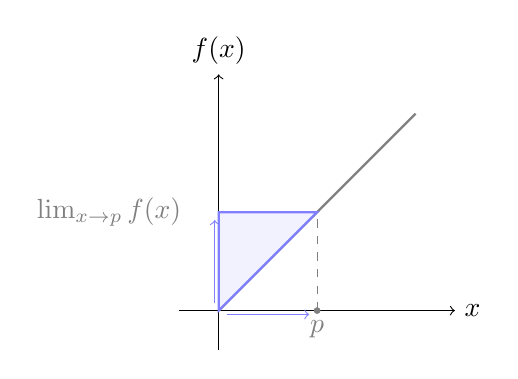
\begin{tikzpicture}[scale=0.5]
            % Assi
            \draw[->] (-1,0) -- (6,0) node[right] {$x$};
            \draw[->] (0,-1) -- (0,6) node[above] {$f(x)$};
            
            % Funzione crescente
            \draw[thick,gray,domain=0:5] plot (\x,{\x});
    
            % Punto p
            \filldraw[color=gray] (2.5,0) circle (2pt) node[below] {$p$};
            \draw[dashed, gray] (2.5,0) -- (2.5,2.5) -- (0,2.5) node[left] {$\lim_{x \to p} f(x)\quad$};
    
            \draw[thick,blue!50,fill=blue!5] (0,0) -- (0,2.5) -- (2.5,2.5) -- cycle;
    
            \draw[->, blue!50] (-0.1,0.2) -- (-0.1,2.3);
            \draw[->, blue!50] (0.2,-0.1) -- (2.3,-0.1);
        \end{tikzpicture}
    \end{figure}
    Se $f$ è decrescente si ha 
    \[\lim_{x\to p^-}f(x)=\inf\{f(x)\,|\,x\in A\,\land\, x<p\}.\]
    \begin{figure}[H]
        \centering
        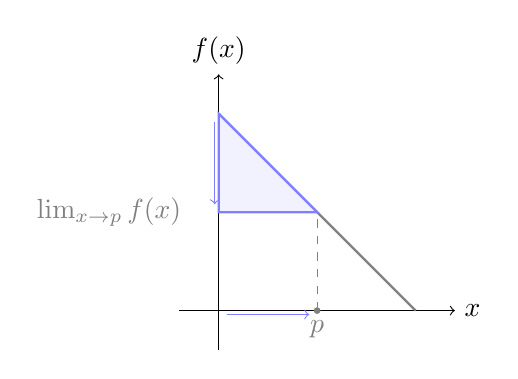
\begin{tikzpicture}[scale=0.5]
            % Assi
            \draw[->] (-1,0) -- (6,0) node[right] {$x$};
            \draw[->] (0,-1) -- (0,6) node[above] {$f(x)$};
            
            % Funzione crescente
            \draw[thick,gray,domain=0:5] plot (\x,{-\x+5});
    
            % Punto p
            \filldraw[color=gray] (2.5,0) circle (2pt) node[below] {$p$};
            \draw[dashed, gray] (2.5,0) -- (2.5,2.5) -- (0,2.5) node[left] {$\lim_{x \to p} f(x)\quad$};
    
            \draw[thick,blue!50,fill=blue!5] (0,2.5) -- (0,5) -- (2.5,2.5) -- cycle;
            \draw[->, blue!50] (-0.1,4.8) -- (-0.1,2.7);
            \draw[->, blue!50] (0.2,-0.1) -- (2.3,-0.1);
        \end{tikzpicture}
    \end{figure}
\end{thm}
\end{bxthm}

\vspace{10pt}

\begin{bxthm}
\begin{thm}
    Siano $f:A\to\mathbb{R}$ monotòna e $p\in\overline{\mathcal{D}^+}(A)$.
    Allora il limite da destra di $f$ in $p$ esiste sempre.
    Più precisamente, se $f$ è crescente, si ha 
    \[\lim_{x\to p^+}f(x)=\inf\{f(x)\,|\,x\in A\,\land\, x>p\}.\]
    \begin{figure}[H]
        \centering
        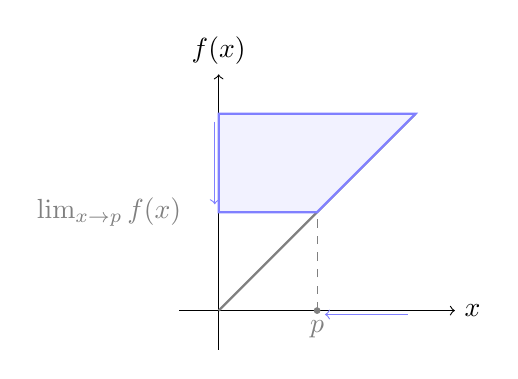
\begin{tikzpicture}[scale=0.5]
            % Assi
            \draw[->] (-1,0) -- (6,0) node[right] {$x$};
            \draw[->] (0,-1) -- (0,6) node[above] {$f(x)$};
            
            % Funzione crescente
            \draw[thick,gray,domain=0:5] plot (\x,{\x});
    
            % Punto p
            \filldraw[color=gray] (2.5,0) circle (2pt) node[below] {$p$};
            \draw[dashed, gray] (2.5,0) -- (2.5,2.5) -- (0,2.5) node[left] {$\lim_{x \to p} f(x)\quad$};
    
            \draw[thick,blue!50,fill=blue!5] (0,2.5) -- (0,5) -- (5,5) -- (2.5,2.5) -- cycle;
    
            \draw[->, blue!50] (-0.1,4.8) -- (-0.1,2.7);
            \draw[->, blue!50] (4.8,-0.1) -- (2.7,-0.1);
        \end{tikzpicture}
    \end{figure}
    Se $f$ è decrescente si ha 
    \[\lim_{x\to p^+}f(x)=\sup\{f(x)\,|\,x\in A\,\land\, x>p\}.\]
    \begin{figure}[H]
        \centering
        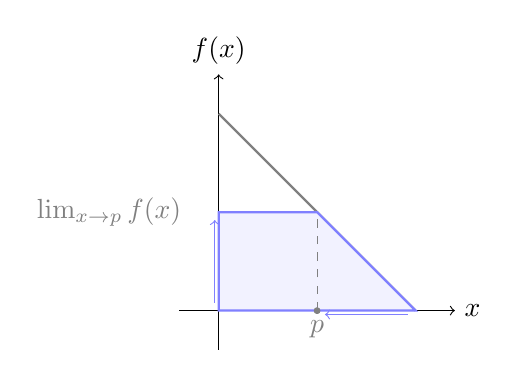
\begin{tikzpicture}[scale=0.5]
            % Assi
            \draw[->] (-1,0) -- (6,0) node[right] {$x$};
            \draw[->] (0,-1) -- (0,6) node[above] {$f(x)$};
            
            % Funzione crescente
            \draw[thick,gray,domain=0:5] plot (\x,{-\x+5});
    
            % Punto p
            \filldraw[color=gray] (2.5,0) circle (2pt) ;
            \draw[dashed, gray] (2.5,0) -- (2.5,2.5) -- (0,2.5) node[left] {$\lim_{x \to p} f(x)\quad$};
    
            \draw[thick,blue!50,fill=blue!5] (0,0) -- (0,2.5) -- (2.5,2.5) -- (5,0) -- cycle;
    
            \draw[dashed, gray] (2.5,0) node[below] {$p$}-- (2.5,2.5) ;
            \filldraw[color=gray] (2.5,0) circle (2pt) ;
            \draw[->, blue!50] (4.8,-0.1) -- (2.7,-0.1);
            \draw[->, blue!50] (-0.1,0.2) -- (-0.1,2.3);
            
        \end{tikzpicture}
    \end{figure}
\end{thm}
\end{bxthm}

\vspace{10pt}

\subsection{Classificazione dei punti di discontinuità mediante i limiti}

\vspace{10pt}

\begin{bxthm}
\begin{defn}
    Sia $f:A\to\mathbb{R}$ discontinua in $w\in A$ con $w\in \mathcal{D}(A)$.
    Diciamo che la discontinuità è di $1^\circ$ specie:
    \begin{itemize}
        \item \textbf{Eliminabile: } se \[\lim_{x\to w}f(x)=l\in\mathbb{R}\quad\textup{ e }\quad l\neq f(w);\]
        \item \textbf{Non eliminabile: } se il limite non esiste, ma \[w\in\mathcal{D}^-(A)\cap\mathcal{D}^+(A)\]
        ed esistono e sono finiti i seguenti limiti:
         \[\lim_{x\to w^-}f(x)=l'\in\mathbb{R}\;\textup{ e }\lim_{x\to w^+}f(x)=l''\in\mathbb{R}\quad\textup{con }l'\neq l''.\]
    \end{itemize}
\end{defn}
\end{bxthm}

\vspace{10pt}

\subsection{Teorema della permanenza del segno per i limiti di funzioni}

\vspace{10pt}

\begin{bxthm}
\begin{thm}
    Sia $f:A\to\mathbb{R}$ con $p\in\overline{\mathcal{D}}(A)$, e supponiamo che 
    \[\lim_{x\to p}f(x)=l\in\overline{\mathbb{R}}\] con $l>0$ ($l<0$).
    Allora 
    \[\exists\, I\in \mathcal{I}_p \,:\; \forall\, x\in A\cap I\setminus\{p\},\quad f(x)>0\quad(f(x)<0).\]
\end{thm}
\end{bxthm}
\begin{proof}
    Sia $J\in \mathcal{I}_l$ contenuto in $]0,+\infty[$ 
    \begin{itemize}
        \item Se abbiamo $l\in\mathbb{R}$, allora prendiamo \[J=\,]l-\varepsilon,l+\varepsilon[\textup{ con }\varepsilon=l;\]
        \item Se abbiamo $l=+\infty$, allora ogni $J\in \mathcal{I}_l$ va bene.
    \end{itemize}
    Per ipotesi, 
    \[\exists\, I\in \mathcal{I}_p\,:\,f(A\cap I\setminus\{p\})\subseteq J\subseteq\, ]0,+\infty[,\]
    pertanto 
    \[\forall\, x\in A\cap I\setminus\{p\},\quad f(x)>0.\]
\end{proof}

\vspace{10pt}

\subsection{Teorema del confronto}

\vspace{10pt}

\begin{bxthm}
\begin{thm}
    Siano $f,g:A\to\mathbb{R}$ e $p\in\overline{\mathcal{D}}(A)$, e supponiamo che esistano i limiti di $f$ e $g$ in $p$. 
    Se l'insieme $E=\{x\in A \,|\, f(x)\leq g(x)\}$ ha $p$ come punto di accumulazione, ovvero
    \[\exists\, H\in \mathcal{I}_p\,:\;\forall\, x\in A\cap H\setminus\{p\},\quad f(x)\leq g(x),\]
    allora \[\lim_{x\to p}f(x)\,\leq\, \lim_{x\to p}g(x).\]
\end{thm}
\end{bxthm}
\begin{proof}
    Sia 
    \[h:A\to\mathbb{R}\quad x\mapsto f(x)-g(x),\]
    e supponiamo che 
    \[\lim_{x\to p}f(x)=l \quad\land\quad \lim_{x\to p}g(x)=m\quad \textup{con }l>m,\]
    allora \[\lim_{x\to p}h(x)=l-m>0,\] quindi per il teorema precedente abbiamo che 
    \[\exists\, I\in \mathcal{I}_p \,:\;\forall\, x\in A\cap I\setminus\{p\},\quad h(x)>0\]
    da cui \[f(x)-g(x)>0\quad\implies\quad f(x)>g(x).\]
    Pertanto \[E\cap I\setminus\{p\}=\emptyset\quad\implies\quad p\notin\overline{\mathcal{D}}(E)\]
\end{proof}

\vspace{10pt}

\subsection{Teorema dei carabinieri}

\vspace{10pt}

\begin{bxthm}
\begin{thm}
    Siano $f,g,h:A\to\mathbb{R}$ e $p\in\overline{\mathcal{D}}(A)$.
    Supponiamo che 
    \[\lim_{x\to p}f(x)=\lim_{x\to p}h(x)=l\in\overline{\mathbb{R}}.\]
    Se \[\exists\, H\in \mathcal{I}_p\,:\;\forall\, x\in A\cap H\setminus\{p\},\quad f(x)\leq g(x)\leq h(x),\]
    Allora \[\lim_{x\to p}g(x)=l.\]
\end{thm}
\end{bxthm}
\begin{proof}
    Fissiamo $\varepsilon>0$.
    Per ipotesi trovo $I',I''\in \mathcal{I}_p$ tali che 
    \[f(A\cap I'\setminus\{p\})\subseteq\,]\,l-\varepsilon,l+\varepsilon\,[\quad\textup{e}\quad h(A\cap I''\setminus\{p\})\subseteq\,]\,l-\varepsilon,l+\varepsilon\,[.\]
    Sia $I=I'\cap I''\cap H$, allora 
    \[\forall\, x\in A\cap I\setminus\{p\},\quad l-\varepsilon<f(x)\leq g(x)\leq h(x)<l+\varepsilon,\]
    cioè \[g(A\cap I\setminus\{p\})\subseteq\,]\,l-\varepsilon,l+\varepsilon\,[.\]
\end{proof}

\vspace{50pt}
\section{Successioni}
\vspace{50pt}

\subsection{Successioni}

\vspace{10pt}

\paragraph{Successione}
\begin{bxthm}
\begin{defn}
    Si definisce \textbf{successione} una funzione 
    \[s:\mathbb{N}\to A\subseteq\mathbb{R}\quad n\mapsto s(n).\]
\end{defn}
\end{bxthm}

\vspace{10pt}

\paragraph{Successione numerica reale}
\begin{bxthm}
\begin{defn}
    Si definisce \textbf{successione numerica reale} una successione a valori in $\mathbb{R}$.
    \[s:\mathbb{N}\to \mathbb{R}\quad n\mapsto s(n).\]
    Scriveremo \[(s_n)_{n\in\mathbb{N}}.\]
\end{defn}
\end{bxthm}

\vspace{10pt}

\begin{note}
Le successioni si possono rappresentare anche in questo modo:
\[(1,1),\,(2,2),\,(3,3),\,\cdots,\,(n,n),\,\cdots\]
In cui ciascun elemento (coppia) viene chiamato \textbf{termine}, il primo elemento viene chiamato \textbf{indice} e il secondo elemento viene chiamato \textbf{valore}.
\[(1,s_1),\,(2,s_2),\,(3,s_3),\,\cdots,\,(n,s_n),\,\cdots\]
Oppure in quest'altro modo
\[(s_1,s_2,s_3,...,s_n,...)=(s_n)_{n\in\mathbb{N}}\]
La differenza tra un'insieme e una successione è che nell'insieme gli elementi non si possono mai ripetere, nelle successioni invece può accadere.
\end{note}

\vspace{10pt}

\begin{note}
    Non esistono punti di accumulazione, perchè sono isolati. L'unico punto di accumulazione è il limite $+\infty$.
\end{note}

\vspace{10pt}

\subsection{Limiti di successioni}

\vspace{10pt}

\paragraph{Limite convergente di una successione}
\begin{bxthm}
\begin{defn}
    Sia $(s_n)_{n\in\mathbb{N}}$ una successione numerica reale; diremo che il \textbf{limite} per $n\to+\infty$ di $s_n$ vale $l\in\mathbb{R}$ e scriveremo 
    \[\lim_{n\to+\infty}s_n=l\]
    se 
    \[\forall\,\varepsilon>0,\;\exists\,v\in\mathbb{N}\,|\,\forall\,n\in\mathbb{N},\quad n>v\implies |s_n-l|<\varepsilon.\]
    In questo caso la successione si dice \textbf{convergente}.
\end{defn}
\end{bxthm}

\vspace{10pt}

\paragraph{Limite divergente di una successione}
\begin{bxthm}
\begin{defn}
    Sia $(s_n)_{n\in\mathbb{N}}$ una successione numerica reale; diremo che la successione
    \begin{itemize}
        \item \textbf{Diverge positivamente}, e scriveremo $\lim_{n\to+\infty}s_n=+\infty$, se \[\forall\,M>0,\;\exists\,v\in\mathbb{N}\,:\,\forall\,n>v,\quad s_n>M\]
        \item \textbf{Diverge negativamente}, e scriveremo $\lim_{n\to+\infty}s_n=-\infty$ se \[\forall\,M>0,\;\exists\,v\in\mathbb{N}\,:\,\forall\,n>v,\quad s_n<-M\]
        \item \textbf{Oscilla}, e scriveremo $\lim_{n\to+\infty}s_n=\infty$ se \[\forall\,M>0,\;\exists\,v\in\mathbb{N}\,:\,\forall\,n>v,\quad |s_n|>M\]
    \end{itemize}
\end{defn}
\end{bxthm}

\vspace{10pt}

\paragraph{Definitivamente}
\begin{bxthm}
\begin{defn}
    Sia $P(n)$ una proprietà che dipende da $n\in\mathbb{N}$, diremo che $P(n)$ vale \textbf{definitivamente} se
    \[\exists\,v\in\mathbb{N}\,:\;\forall\,n\geq v,\quad P(n)\;\textup{è vera}.\]
\end{defn}
\end{bxthm}

\vspace{10pt}

\begin{bxthm}
\begin{thm}
    Sia $s_n$ una successione numerica reale. Allora le seguenti scritture sono equivalenti.
    \begin{enumerate}
        \item $\lim_{n\to+\infty}s_n=l$;
        \item $s_n$ è definitivamente in ogni intorno di $l$.
    \end{enumerate}
\end{thm}
\end{bxthm}
\begin{proof}
    La scrittura $\lim_{n\to+\infty}s_n=l$ significa
    \[\forall\, J\in \mathcal{I}_l,\;\exists\, M>0\,:\;\forall\, n\in\mathbb{N},\quad(n>M\;\implies\; s_n\in J).\]
    $s_n$ è definitivamente in ogni intorno di $l$ significa 
    \[\forall\, J\in \mathcal{I}_l,\;\exists\, v\in\mathbb{N}\,:\;\forall\, n\in\mathbb{N},\quad (n\geq v\;\implies\; s_n\in J).\]
    Dunque le due scritture si equivalgono se prendiamo \[M=v-\dfrac{1}{2}.\]
\end{proof}

\vspace{10pt}

\paragraph{Frequentemente}
\begin{bxthm}
\begin{defn}
    Sia $P(n)$ una proprietà che dipende da $n\in\mathbb{N}$, diremo che $P(n)$ vale \textbf{frequentemente} se
    \[\forall\,k\in\mathbb{N}\,:\;\exists\,n\geq k,\quad P(n)\;\textup{è vera}.\]
\end{defn}
\end{bxthm}

\vspace{10pt}

\begin{exmp}
    Sia \(\forall\, n\in\mathbb{N},\, s_n=(-1)^n,\) allora $(s_n)_{n\in\mathbb{N}}$ è:
    \begin{itemize}
        \item \textbf{frequentemente} positiva perchè 
        \[\forall\, k\in\mathbb{N},\;\exists\, n\geq k\,:\,(s_n)_{n\in\mathbb{N}}>0.\]
        Ad esempio per $k=3$, prendiamo $n=4$ a cui corrisponde $(s_n)_{n\in\mathbb{N}}=1>0$ e così via per ogni $k$ dispari.
        \item \textbf{frequentemente} negativa perchè 
        \[\forall\, k\in\mathbb{N},\;\exists\, n\geq k\,:\,(s_n)_{n\in\mathbb{N}}<0.\]
        Ad esempio per $k=4$, prendiamo $n=5$ a cui corrisponde $(s_n)_{n\in\mathbb{N}}=-1<0$ e così via per ogni $k$ pari.\\
    \end{itemize}

    \begin{center}
        \centering 
        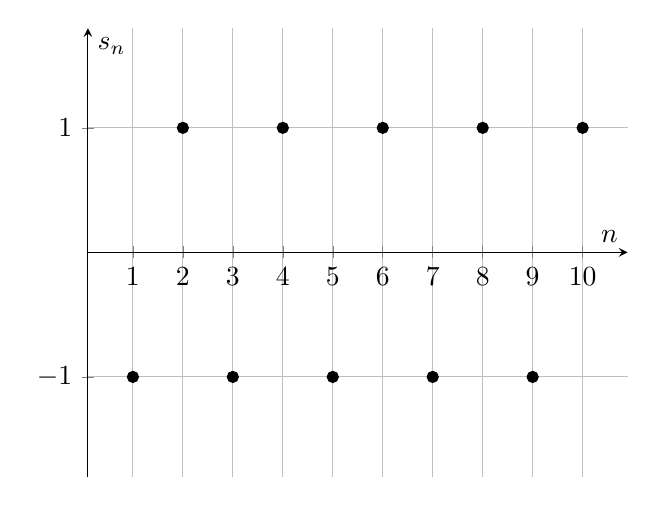
\begin{tikzpicture}
            \begin{axis}[
                xlabel={$n$},
                ylabel={$s_n$},
                grid=major,
                domain=1:10,
                samples=10,
                ytick={-1, 0, 1},
                xtick={1, 2, ..., 10},
                ymin=-1.5, ymax=1.5,
                xmin=1, xmax=10,
                axis x line=middle,
                axis y line=middle,
                enlargelimits,
            ]
            \addplot[
                only marks,
                mark=*,
                mark size=2pt,
            ] coordinates {
                (1, -1) (2, 1) (3, -1) (4, 1) (5, -1)
                (6, 1) (7, -1) (8, 1) (9, -1) (10, 1)
            };
            \end{axis}
        \end{tikzpicture}
    \end{center}
\end{exmp}

\vspace{10pt}

\paragraph{Caratterizzazione delle successioni monotòne}
\begin{bxthm}
\begin{thm}
    $\forall\, n\in\mathbb{N},$ una successione $(s_n)_{n\in\mathbb{N}}$ è:
    \begin{itemize}
        \item \textbf{crescente} se e solo se 
        \[s_n\leq s_{n+1}\]
        \item \textbf{strettamente crescente} se e solo se 
        \[s_n<s_{n+1}\]
        \item \textbf{decrescente} se e solo se 
        \[s_n\geq s_{n+1}\]
        \item \textbf{strettamente decrescente} se e solo se 
        \[s_n>s_{n+1}\]
    \end{itemize}
\end{thm}
\end{bxthm}
\begin{proof}
    La necessità è ovvia (perchè $n<n+1$).
    Supponiamo quindi \[\forall\,n\in\mathbb{N},\quad s_n\leq s_{n+1},\]  e siano $n',n''\in\mathbb{N}$ con $n'<n''$.
    Posto $h=n''-n'$, si ha $h\in\mathbb{N}$, quindi possiamo procedere per induzione su $h$.
    \begin{itemize}
        \item[$h=1$] Si ha \[n''=n'+h=n'+1,\] per cui \[s_{n'}\leq s_{n'+1}=s_{n''}\]
        \item[$h\rightsquigarrow h+1$] l'ipotesi induttiva è che \[s_{n'+h}\geq s_{n'},\] pertanto \[s_{n'+h+1}=s_{(n'+h)+1}\geq s_{n'+h}\geq s_{n'}.\]
    \end{itemize}
\end{proof}

\vspace{10pt}

\paragraph{Costruzione del numero $e$}
\begin{bxthm}
\begin{thm}
    \[e=\lim_{n\to+\infty}\left(1+\dfrac{1}{n}\right)^{n+1}.\]
\end{thm}
\end{bxthm}
\begin{proof}
    Sia \[\forall\, n\in\mathbb{N},\quad b_n=\left(1+\dfrac{1}{n}\right)^{n+1}.\]
    Mostriamo che la successione $(b_n)_{n\in\mathbb{N}}$ è strettamente decrescente, e precisamente che 
    \[\forall\, n\in\mathbb{N},\quad\dfrac{b_n}{b_{n+1}}>1\]
    \begin{align*}
        \dfrac{b_n}{b_{n+1}}=&\,\dfrac{\left(1+\dfrac{1}{n}\right)^{n+1}}{\left(1+\dfrac{1}{n+1}\right)^{n+2}}=\dfrac{\left(\dfrac{n+1}{n}\right)^{n+1}}{\left(\dfrac{n+2}{n+1}\right)^{n+2}}=\dfrac{1}{\dfrac{n+2}{n+1}}\left(\dfrac{\dfrac{n+1}{n}}{\dfrac{n+2}{n+1}}\right)^{n+1}=\dfrac{n+1}{n+2}\left(\dfrac{(n+1)^2}{n(n+2)}\right)^{n+1}\\\\
        =&\,\dfrac{n+1}{n+2}\left(\dfrac{n^2+2n+1}{n^2+2n}\right)^{n+1}=\dfrac{n+1}{n+2}\left(1+\dfrac{1}{n^2+2n}\right)^{n+1}\\
    \end{align*}
    A questo punto poniamo $b=\dfrac{1}{n^2+2n}$ e $m=n+1$, per la disuguaglianza di Bernoulli avremo
    \[\left(1+\dfrac{1}{n^2+2n}\right)^{n+1}=(1+b)^m\geq1+mb=\left(1+(n+1)\dfrac{1}{n^2+2n}\right),\]
    da cui
    \begin{align*}
        &\dfrac{n+1}{n+2}\left(1+\dfrac{1}{n^2+2n}\right)^{n+1}\geq\dfrac{n+1}{n+2}\left(1+(n+1)\dfrac{1}{n^2+2n}\right)=\dfrac{n+1}{n+2}\left(1+\dfrac{n+1}{n^2+2n}\right)\\\\
        =&\,\dfrac{n+1}{n+2}\dfrac{n^2+3n+1}{n(n+2)}=\dfrac{(n+1)(n^2+3n+1)}{n(n+2)^2}=\dfrac{n^3+4n^2+4n+1}{n(n^2+4n+4)}\\\\
        =&\,\dfrac{n^3+4n^2+4n+1}{n^3+4n^2+4n}=\dfrac{\cancel{n^3+4n^2+4n}}{\cancel{n^3+4n^2+4n}}+\dfrac{1}{n^3+4n^2+4n}=1+\dfrac{1}{n^3+4n^2+4n}>1\\\\
    \end{align*}
\end{proof}

\vspace{10pt}

\begin{center}
    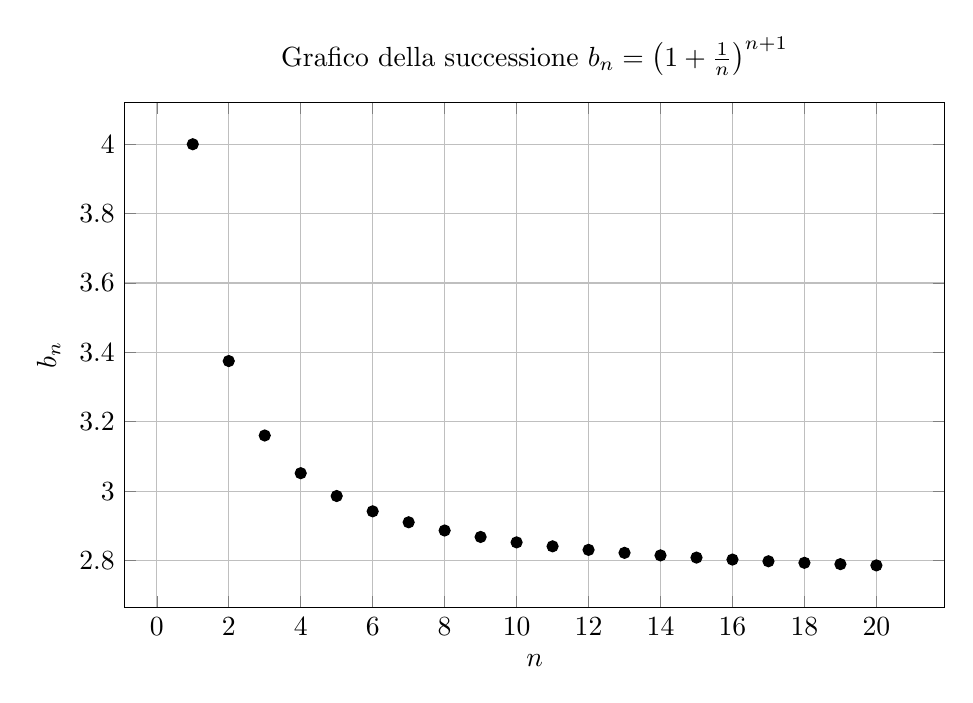
\begin{tikzpicture}
        \begin{axis}[
            xlabel={$n$},
            ylabel={$b_n$},
            title={Grafico della successione $b_n = \left(1 + \frac{1}{n}\right)^{n+1}$},
            grid=major,
            width=12cm,
            height=8cm
        ]
            \addplot[only marks, mark=*, color=black] coordinates {
                (1, 4.0000)
                (2, 3.3750)
                (3, 3.1604)
                (4, 3.0517)
                (5, 2.9859)
                (6, 2.9418)
                (7, 2.9102)
                (8, 2.8865)
                (9, 2.8679)
                (10, 2.8523)
                (11, 2.8409)
                (12, 2.8307)
                (13, 2.8221)
                (14, 2.8148)
                (15, 2.8084)
                (16, 2.8027)
                (17, 2.7978)
                (18, 2.7934)
                (19, 2.7895)
                (20, 2.7859)
            };
        \end{axis}
    \end{tikzpicture}
\end{center}

\vspace{10pt}

\begin{bxthm}
\begin{cor}
    \[e=\lim_{n\to+\infty}\left(1+\dfrac{1}{n}\right)^n.\]
\end{cor}
\end{bxthm}
\begin{proof}
    Sia \[\forall\, n\in\mathbb{N},\quad a_n=\left(1+\dfrac{1}{n}\right)^n.\]
    Si ha \[b_n=a_n\left(1+\dfrac{1}{n}\right),\] quindi \[a_n=\dfrac{b_n}{1+\frac{1}{n}},\]
    ma \[\lim_{n\to+\infty}\dfrac{1}{n}=0 \quad\therefore\quad \lim_{n\to+\infty}\dfrac{b_n}{1+\frac{1}{n}}=\dfrac{e}{1+0}=e.\]
\end{proof}

\vspace{10pt}

\begin{center}
    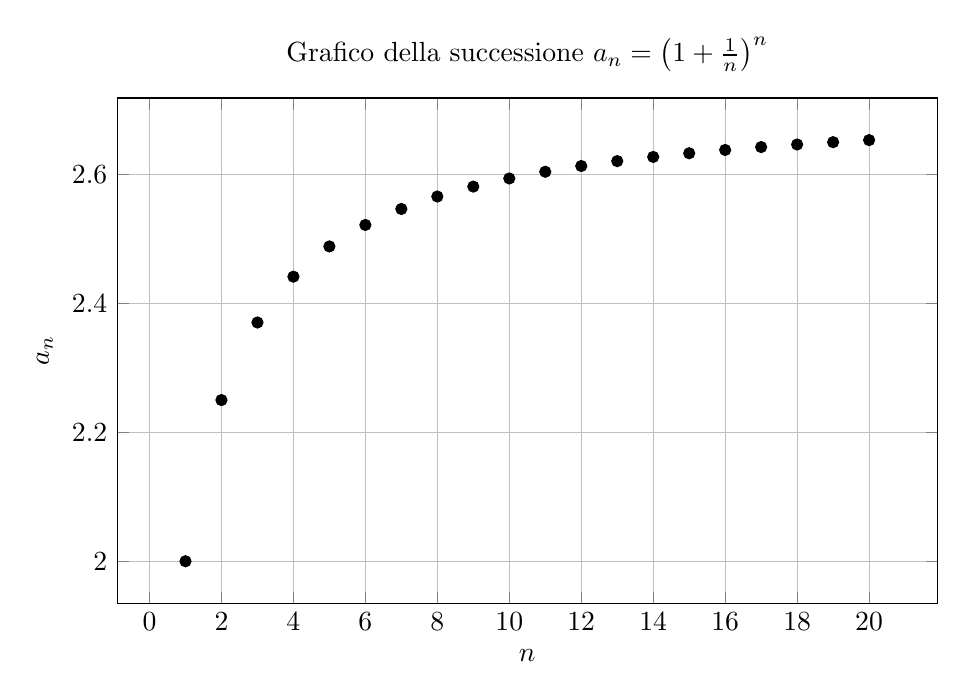
\begin{tikzpicture}
        \begin{axis}[
            xlabel={$n$},
            ylabel={$a_n$},
            title={Grafico della successione $a_n = \left(1 + \frac{1}{n}\right)^{n}$},
            grid=major,
            width=12cm,
            height=8cm
        ]
            \addplot[only marks, mark=*, color=black] coordinates {
                (1, 2.0000)
                (2, 2.25)
                (3, 2.3703)
                (4, 2.4414)
                (5, 2.4883)
                (6, 2.5216)
                (7, 2.5464)
                (8, 2.5657)
                (9, 2.5811)
                (10, 2.5937)
                (11, 2.6041)
                (12, 2.613)
                (13, 2.6206)
                (14, 2.6271)
                (15, 2.6328)
                (16, 2.6379)
                (17, 2.6424)
                (18, 2.6464)
                (19, 2.65)
                (20, 2.6532)
            };
        \end{axis}
    \end{tikzpicture}
\end{center}

\vspace{10pt}

\begin{bxthm}
\begin{thm}
    \[\lim_{x\to+\infty}\left(1+\frac{1}{x}\right)^x=e.\]
\end{thm}
\end{bxthm}
\begin{proof}
    Sia $n=\lfloor x\rfloor$. Supponiamo $x\geq1$ cosicchè $n\in\mathbb{N}$.
    Si ha $n\leq x<n+1$, pertanto 
    \[\dfrac{1}{n+1}<\dfrac{1}{x}\;\leq\;\dfrac{1}{n},\] da cui
    \[\left(1+\frac{1}{n+1}\right)^n\leq\left(1+\frac{1}{n+1}\right)^x<\left(1+\frac{1}{x}\right)^x\leq\left(1+\frac{1}{n}\right)^x<\left(1+\frac{1}{n}\right)^{n+1}.\]\\
    Fissato $\varepsilon>0$, siano 
    \begin{itemize}
        \item $\nu_1\in\mathbb{N}$ tale che, per $n\geq\nu_1$, si abbia \[\left(1+\dfrac{1}{n+1}\right)^n\in\;]e-\varepsilon,e+\varepsilon[\]
        \item $\nu_2\in\mathbb{N}$ tale che, per $n\geq\nu_2$, si abbia \[\left(1+\dfrac{1}{n}\right)^{n+1}\in\;]e-\varepsilon,e+\varepsilon[.\]
    \end{itemize}
    Poniamo dunque \[M=1+\max\{\nu_1,\nu_2\}\;(>0).\]
    Se $x>M$, essendo 
    \[n>x-1>M-1=\max\{\nu_1,\nu_2\},\]si ha \[n>\nu_1\quad\textup{e}\quad n>\nu_2.\] 
    Quindi 
    \[\left(1+\frac{1}{n+1}\right)^n>e-\varepsilon\quad\textup{e}\quad\left(1+\frac{1}{n}\right)^{n+1}<e+\varepsilon.\]
    Concludiamo che \[e-\varepsilon<\left(1+\frac{1}{x}\right)^x<e+\varepsilon.\]
\end{proof}

\vspace{10pt}

\paragraph{Dimostrazioni di alcuni limiti notevoli}
\begin{enumerate}
    \item \[\lim_{x\to0}\dfrac{\sin x}{x}=1\] 
    \begin{proof}
        Per ogni \( x \in \left]0, \frac{\pi}{2}\right[, \) abbiamo che:
        \[
        \sin x < x < \tan x = \frac{\sin x}{\cos x}.
        \]
        Dunque:
        \[
        1 < \dfrac{x}{\sin x} < \dfrac{1}{\cos x} \quad \implies \quad \cos x < \dfrac{\sin x}{x} < 1.
        \]
        Da cui segue:
        \[
        \lim_{x \to 0^+} \dfrac{\sin x}{x} = 1 \quad \text{e} \quad \lim_{x \to 0^-} \dfrac{\sin x}{x} = 1.
        \]
        Poniamo \( t = -x \). Quando \( x \to 0^- \), si ha che \( t \to 0^+ \). Pertanto:
        \[
        \lim_{t \to 0^+} \dfrac{\sin(-t)}{-t} = \lim_{t \to 0^+} \dfrac{\sin t}{t} = 1.
        \]
    \end{proof}
    \item \[\lim_{x\to-\infty}\left(1+\frac{1}{x}\right)^x=e\]
    \begin{proof}
        Sia \( t = -1 - x \). Allora \( x = -1 - t \), e quando \( x \to -\infty \), si ha che \( t \to +\infty \). Dunque, abbiamo:
        \[
        \lim_{x \to -\infty}\left(1 + \dfrac{1}{x}\right)^x = \lim_{t \to +\infty}\left(1 + \dfrac{1}{-1 - t}\right)^{-1 - t}.
        \]
        Questo si semplifica in:
        \[
        \lim_{t \to +\infty}\left(1 - \dfrac{1}{1 + t}\right)^{-(1 + t)} = \lim_{t \to +\infty}\left(\dfrac{1 + t - 1}{1 + t}\right)^{-(1 + t)} = \lim_{t \to +\infty}\left(\dfrac{t}{1 + t}\right)^{-(1 + t)}.
        \]
        Successivamente:
        \[
        \lim_{t \to +\infty}\left(\dfrac{1 + t}{t}\right)^{(1 + t)} = \lim_{t \to +\infty}\left(1 + \dfrac{1}{t}\right)^{(1 + t)}.
        \]
        Osserviamo che:
        \[
        \lim_{t \to +\infty}\left(1 + \dfrac{1}{t}\right)^{(1 + t)} = \lim_{t \to +\infty}\left[\left(1 + \dfrac{1}{t}\right)^t\left(1 + \dfrac{1}{t}\right)\right].
        \]
        Poiché \( \left(1 + \dfrac{1}{t}\right)^t \to e \) quando \( t \to +\infty \), abbiamo:
        \[
        \lim_{t \to +\infty}\left(1 + \dfrac{1}{t}\right)^t = e.
        \]
        E dato che \( \left(1 + \dfrac{1}{t}\right) \to 1 \) quando \( t \to +\infty \), otteniamo:
        \[
        \lim_{t \to +\infty}\left(1 + \dfrac{1}{t}\right) = 1.
        \]
        Pertanto:
        \[
        \lim_{t \to +\infty}\left(1 + \dfrac{1}{t}\right)^{(1 + t)} = e \cdot 1 = e.
        \]
    \end{proof}
    \item \[\lim_{x\to0}\dfrac{1-\cos x}{x^2}=\dfrac{1}{2}\]
    \begin{proof}
        Consideriamo:
        \[
        \lim_{x \to 0}\dfrac{1-\cos x}{x^2} \cdot \dfrac{1+\cos x}{1+\cos x}.
        \]
        Questo si semplifica in:
        \[
        \lim_{x \to 0}\dfrac{1-\cos^2 x}{x^2(1+\cos x)}.
        \]
        Usando l'identità trigonometrica \( 1 - \cos^2 x = \sin^2 x \), otteniamo:
        \[
        \lim_{x \to 0}\dfrac{\sin^2 x}{x^2(1+\cos x)}.
        \]
        Questo si può scrivere come il prodotto di due limiti:
        \[
        \lim_{x \to 0}\dfrac{1}{1+\cos x} \cdot \lim_{x \to 0}\dfrac{\sin^2 x}{x^2}.
        \]
        Calcoliamo il primo limite:
        \[
        \lim_{x \to 0}\dfrac{1}{1+\cos x} = \dfrac{1}{1+1} = \dfrac{1}{2}.
        \]
        Calcoliamo il secondo limite usando \( \left(\dfrac{\sin x}{x}\right)^2 \):
        \[
        \lim_{x \to 0}\dfrac{\sin^2 x}{x^2} = \left(\lim_{x \to 0}\dfrac{\sin x}{x}\right)^2 = 1^2 = 1.
        \]
        Moltiplicando i risultati, otteniamo:
        \[
        \dfrac{1}{2} \cdot 1 = \dfrac{1}{2}.
        \]
        Pertanto:
        \[
        \lim_{x\to0}\dfrac{1-\cos x}{x^2} = \dfrac{1}{2}.
        \]
    \end{proof}
    \item \[\lim_{x\to0}\dfrac{\ln(1+x)}{x}=1\]
    \begin{proof}
        Poniamo \( t = \dfrac{1}{x} \). Allora 
        \[x=\dfrac{1}{t}\;\therefore\;\begin{cases}x\to0^+\;\implies\; t\to+\infty\\ x\to0^-\;\implies\; t\to-\infty\end{cases}\]

        Consideriamo il caso \( x \to 0^+ \):
        \[
        \lim_{x\to0^+}\dfrac{\ln(1+x)}{x} = \lim_{t\to+\infty}\dfrac{\ln\left(1+\frac{1}{t}\right)}{\frac{1}{t}}.
        \]
        Questo si semplifica in:
        \[
        \lim_{t\to+\infty} t \ln\left(1+\dfrac{1}{t}\right).
        \]
        Applicando il limite, otteniamo:
        \[
        \lim_{t\to+\infty} \ln\left( \left(1+\dfrac{1}{t}\right)^t \right).
        \]
        Poiché \( \left(1 + \dfrac{1}{t}\right)^t \to e \) quando \( t \to +\infty \), abbiamo:
        \[
        \ln\left(\lim_{t\to+\infty}\left(1+\dfrac{1}{t}\right)^t\right) = \ln e = 1.
        \]
    
        Consideriamo ora il caso \( x \to 0^- \):
        \[
        \lim_{x\to0^-}\dfrac{\ln(1+x)}{x} = \lim_{t\to-\infty}\dfrac{\ln\left(1+\frac{1}{t}\right)}{\frac{1}{t}}.
        \]
        Questo si semplifica in:
        \[
        \lim_{t\to-\infty} t \ln\left(1+\dfrac{1}{t}\right).
        \]
        Applicando il limite, otteniamo:
        \[
        \lim_{t\to-\infty} \ln\left( \left(1+\dfrac{1}{t}\right)^t \right).
        \]
        Poiché \( \left(1 + \dfrac{1}{t}\right)^t \to e \) quando \( t \to -\infty \), abbiamo:
        \[
        \ln\left(\lim_{t\to-\infty}\left(1+\dfrac{1}{t}\right)^t\right) = \ln e = 1.
        \]
    
        Pertanto, in entrambi i casi, otteniamo:
        \[
        \lim_{x\to0}\dfrac{\ln(1+x)}{x}=1.
        \]
    \end{proof}
    \item \[\lim_{x\to0}\dfrac{\tan x}{x}=1\]
    \begin{proof}
        \[\lim_{x\to0}\dfrac{\tan x}{x}=\lim_{x\to0}\dfrac{\sin x}{x\cos x}=\lim_{x\to0}\dfrac{\sin x}{x}\cdot \lim_{x\to0}\dfrac{1}{\cos x}=1\cdot 1 = 1.\]
    \end{proof}
    \item \[\lim_{x\to0}\dfrac{e^x-1}{x}=1\]
    \begin{proof}
        Poniamo \( t = e^x - 1 \). Allora \( x = \ln(1 + t) \), e quando \( x \to 0 \), si ha che \( t \to 0 \). Pertanto:
        \[
        \lim_{t \to 0}\dfrac{t}{\ln(1+t)}.
        \]
        Sappiamo che:
        \[
        \lim_{t \to 0}\dfrac{\ln(1+t)}{t} = 1.
        \]
        Quindi:
        \[
        \lim_{t \to 0}\dfrac{t}{\ln(1+t)} = \left( \lim_{t \to 0}\dfrac{\ln(1+t)}{t} \right)^{-1} = 1^{-1} = 1.
        \]
    \end{proof}
    \item \[\lim_{x\to0}\dfrac{\arcsin x}{x}=1\]
    \begin{proof}
        Poniamo \( t = \arcsin x \). Allora \( x = \sin t \), e quando \( x \to 0 \), si ha che \( t \to 0 \). Pertanto:
        \[
        \lim_{t \to 0}\dfrac{t}{\sin t}.
        \]
        Sappiamo che:
        \[
        \lim_{t \to 0}\dfrac{\sin t}{t} = 1.
        \]
        Quindi:
        \[
        \lim_{t \to 0}\dfrac{t}{\sin t} = \left( \lim_{t \to 0}\dfrac{\sin t}{t} \right)^{-1} = 1^{-1} = 1.
        \]
    \end{proof}
    \item \[\lim_{x\to1}\dfrac{x^\alpha-1}{x-1}=\alpha\]
    \begin{proof}
        Consideriamo:
        \[
        \lim_{x \to 1}\dfrac{x^\alpha - 1}{x - 1}.
        \]
        Possiamo riscrivere \( x^\alpha \) come \( e^{\alpha \ln x} \). Allora:
        \[
        \lim_{x \to 1}\dfrac{e^{\alpha \ln x} - 1}{x - 1}.
        \]
        Moltiplichiamo numeratore e denominatore per \( \alpha \ln x \):
        \[
        \lim_{x \to 1}\dfrac{(e^{\alpha \ln x} - 1)(\alpha \ln x)}{(x - 1)(\alpha \ln x)}.
        \]
        Sappiamo che \( \lim_{x \to 1} \dfrac{x - 1}{\ln x} = 1 \), quindi:
        \[
        \alpha \lim_{x \to 1}\dfrac{e^{\alpha \ln x} - 1}{\alpha \ln x} \cdot \left( \lim_{x \to 1} \dfrac{x - 1}{\ln x} \right)^{-1}.
        \]
        Poiché \( \lim_{x \to 1} \dfrac{e^{\alpha \ln x} - 1}{\alpha \ln x} = 1 \), otteniamo:
        \[
        \alpha \cdot 1 \cdot 1 = \alpha.
        \]
        Pertanto:
        \[
        \lim_{x \to 1}\dfrac{x^\alpha - 1}{x - 1} = \alpha.
        \]
    \end{proof}
\end{enumerate}

\vspace{10pt}

\subsection{Caratterizzazioni e collegamenti mediante successioni}

\vspace{10pt}

\paragraph{Caratterizzazione dei punti di accumulazione mediante le successioni}
\begin{bxthm}
\begin{thm}\label{prec}
    Siano $p\in \overline{\mathbb{R}}$ e $A\subseteq\mathbb{R}$. Allora :
    \[p\in\overline{\mathcal{D}}(A)\iff\exists\, (s_n)\in A\setminus\{p\}\textup{ con }\lim\limits_{n\to+\infty}s_n=p.\]
\end{thm}
\end{bxthm}
\begin{proof}\hfill
    \begin{itemize}
        \item[$\implies$]
        Per ogni $n\in \mathbb{N}$, si scelga \[s_n\in I_p\left(\dfrac{1}{n}\right)\cap A\setminus\{p\}\]
        che è non vuoto, perchè $p\in\overline{\mathcal{D}}(A)$. 
        La successione $s_n$ ha limite $p$ perchè per ogni $r>0$, trovo $v\in \mathbb{N}$ con $v>\frac{1}{r}$ 
        cosicchè $\frac{1}{v}<r$ e pertanto 
        \[I_p\left(\dfrac{1}{v}\right)\subseteq I_p(r).\]
        Allora 
        \[\forall\,n\geq v,\quad s_n\in I_p\left(\dfrac{1}{n}\right)\subseteq I_p\left(\dfrac{1}{v}\right)\subseteq I_p(r).\]
        Concludiamo \[\lim_{n\to+\infty}s_n=p.\]
        \item[$\impliedby$]
        Siano $(s_n)\in A\setminus\{p\}$ con $\lim\limits_{n\to+\infty}s_n=p$ e $I\in \mathcal{I}_p$. 
        Per ipotesi 
        \[\exists\,v\in \mathbb{N}\,:\,\forall\,n\geq v,\quad s_n\in I.\]
        Ma $s_n\in A\setminus\{p\}$ quindi $I\cap A\setminus\{p\}\neq\emptyset$.
    \end{itemize}
\end{proof}

\vspace{10pt}

\paragraph{Insiemi chiusi, perfetti e discreti}
\begin{bxthm}
\begin{defn}
    Sia $C\subseteq \mathbb{R}$, diciamo che 
    \begin{itemize}
        \item $C$ è \textbf{chiuso} se $\mathcal{D}(C)\subseteq C$;
        \item $C$ è \textbf{perfetto} se $C\subseteq \mathcal{D}(C)$;
        \item $C$ è \textbf{discreto} se $C\cap \mathcal{D}(C)=\emptyset$.
    \end{itemize}
\end{defn}
\end{bxthm}

\vspace{10pt}

\begin{note}
    Un'intervallo aperto è un insieme perfetto, mentre un'intervallo chiuso è un insieme chiuso e perfetto.
\end{note}

\vspace{10pt}

\paragraph{Caratterizzazione degli insiemi chiusi mediante le successioni}
\begin{bxthm}
\begin{prop}
    \[C\subseteq \mathbb{R} \textup{ è chiuso }\iff\forall\,(s_n)\in C\textup{ con } \lim_{n\to+\infty}s_n=p\in\mathbb{R},\quad p\in C.\]
\end{prop}
\end{bxthm}

\vspace{10pt}

\paragraph{Collegamento tra limiti di funzioni e limiti di successioni}
\begin{bxthm}
\begin{thm}
    Siano $f:A\to \mathbb{R}$, $p\in\overline{\mathcal{D}}(A)$, e $l\in \overline{\mathbb{R}}$. Allora
    \begin{enumerate}
        \item[$(a)$] $\lim\limits_{x\to p}f(x)=l;$ 
        \item[$(b)$] $\forall\, (s_n)\in A\setminus\{p\}$ con $\lim\limits_{n\to +\infty}s_n=p,\;\lim\limits_{n\to+\infty}f(s_n)=l.$
    \end{enumerate}
\end{thm}
\end{bxthm}
\begin{proof}\hfill
    \begin{itemize}
        \item[$\lnot(a)\implies\lnot(b)$]
        Per ipotesi \[\exists\,J\in \mathcal{I}_l\,:\,\forall\,I\in\mathcal{I}_p,\quad f(A\cap I\setminus\{p\})\;\cancel{\subseteq}\; J.\]
        In particolare \[\forall\,n\in\mathbb{N},\;\exists\,s_n\in A\cap I_p\,\left(\dfrac{1}{n}\right)\setminus\{p\}\,:\,f(s_n)\;\cancel{\subseteq}\;J.\]
        La successione $(s_n)$ è in $A\setminus\{p\}$ e $\lim\limits_{n\to+\infty}s_n=p$, ma non può essere $\lim\limits_{x\to+\infty}f(s_n)=l$.
        \item[$(a)\implies(b)$]
        Si applica il primo teorema sul limite della composizione
    \end{itemize}
\end{proof}

\vspace{10pt}

\paragraph{Caratterizzazione della continuità mediante le successioni}
\begin{bxthm}
\begin{thm}
    Siano $f:A\to\mathbb{R}$ e $w\in A$. Sono equivalenti:
    \begin{enumerate}
        \item[$(a)$] $f$ è continua in $w$;
        \item[$(b)$] $\forall\,(s_n)\in A$ con $\lim\limits_{n\to+\infty}s_n=w,\;\lim\limits_{n\to+\infty}f(s_n)=f(w).$
    \end{enumerate}
\end{thm}
\end{bxthm}
\begin{proof}\hfill
    \begin{itemize}
        \item[$(b)\implies (a)$]
        Possiamo supporre $w\in \mathcal{D}(A)$ (altrimenti non ci sarebbe nulla da dimostrare).
        In tal caso il teorema precedente ci dice \[\lim_{x\to w}f(x)=f(w),\] cioè $f$ è continua in $w$.
        \item[$(a)\implies(b)$]
        Si applica il secondo teorema sul limite della composizione
    \end{itemize}
\end{proof}

\vspace{10pt}

\subsection{Teoremi sulle successioni}

\vspace{10pt}

\paragraph{Teorema della permanenza del segno per le successioni}
\begin{bxthm}
\begin{thm}
    Sia \(\lim\limits_{n\to+\infty}s_n=l\in \overline{\mathbb{R}}\textup{ con }l>0.\)
    Allora $s_n>0$ definitivamente.
\end{thm}
\end{bxthm}

\vspace{10pt}

\paragraph{Teorema del confronto per le successioni}
\begin{bxthm}
\begin{thm}
    Siano \[\lim_{n\to+\infty}a_n=a\;\textup{ e }\lim_{n\to+\infty}b_n=b.\]
    Se $a_n\leq b_n$ frequentemente, allora $a\leq b$ definitivamente.
\end{thm}
\end{bxthm}

\vspace{10pt}

\paragraph{Teorema dei carabinieri per le successioni}
\begin{bxthm}
\begin{thm}
    Siano $(a_n),(b_n),(c_n)$ successioni tali che 
    \[\lim_{n\to+\infty}a_n = \lim_{n\to+\infty}c_n = l.\]
    Se $a_n\leq b_n\leq c_n$ definitivamente, allora \[\lim_{n\to+\infty}b_n=l.\]
\end{thm}
\end{bxthm}

\vspace{10pt}

\subsection{Sottosuccessioni}

\vspace{10pt}

\paragraph{Sottosuccessione}
\begin{bxthm}
\begin{defn}
    Sia $(s_n)_{n\in \mathbb{N}}$ una successione.
    Una \textbf{sottosuccessione} di (o una \textbf{successione estratta da}) $(s_n)_{n\in \mathbb{N}}$ è la composizione di 
    $(s_{m_k})_{k\in \mathbb{N}}$ dove $(m_k)_{k\in \mathbb{N}}$ è una successione di numeri naturali strettamente crescente.
\end{defn}
\end{bxthm}

\vspace{10pt}

\begin{bxthm}
\begin{lem}
    Sia $(m_k)_{k\in \mathbb{N}}$ una successione di numeri naturali strettamente crescente.
    Allora \[\forall\,k\in\mathbb{N},\quad m_k\geq k.\]
\end{lem}
\end{bxthm}
\begin{proof}
    Per induzione su $k$:
    \begin{itemize}
        \item È ovvio che $m_1\geq 1$
        \item Sia $m_k\geq k$ per un certo $k\in\mathbb{N}$
        Si ha $m_{k+1}>m_k$, quindi $m_{k+1}\geq 1+m_k\geq 1+k=k+1$
    \end{itemize}
\end{proof}

\vspace{10pt}

\begin{note}
    Nelle precedenti ipotesi \[\lim_{k\to+\infty}m_k=+\infty.\]
\end{note}

\vspace{10pt}

\paragraph{Limite di una sottosuccessione}
\begin{bxthm}
\begin{prop}
    Sia \[\lim_{n\to+\infty}s_n=l\in\overline{\mathbb{R}},\]
    allora 
    \[\forall\,(s_{n_k})_{k\in \mathbb{K}},\quad\lim_{k\to+\infty}s_{n_k}=l.\]
\end{prop}
\end{bxthm}
\begin{proof}
    Si applica il primo teorema della composizione
\end{proof}

\vspace{10pt}

\begin{bxthm}
\begin{thm}
    Ogni successione ha un'estratta monotòna.
\end{thm}
\end{bxthm}
\begin{proof}
    Data la successione $(s_n)_{n\in \mathbb{N}}$, poniamo \[P=\{\,p\in \mathbb{N} \;|\; \forall\, n>p,\; s_n\leq s_p\}\] e distinguiamo due casi.
    \begin{enumerate}
        \item $P$ è finito, cioè limitato superiormente.
        Definiamo per ricorrenza una successione $(m_k)_{k\in \mathbb{N}}$ di numeri naturali come segue: 
        \[\exists\, m_1\in \mathbb{N} \,:\; \forall\, p\in P,\quad p<m_1.\]
        Supponiamo ora di aver definito $m_k\in \mathbb{N}$ con $p<m_k$ $\forall\, p\in P$, e prendiamo 
        \[m_{k+1}>m_k\textup{ con }s_{m_{k+1}}>s_{m_{k}}.\] 
        Perchè $(m_k)_{k\in \mathbb{N}}$ è strettamente crescente, quindi $(s_{m_k})$ è una sottosuccessione di $(s_m)_{m\in \mathbb{N}}$, ed è monotòna, e precisamente strettamente crescente grazie a \[s_{m_{k+1}}>s_{m_{k}}.\]
        \item $P$ è infinito, cioè illimitato superiormente. 
        Definiamo per ricorrenza una successione $(m_k)_{k\in \mathbb{N}}$ di numeri naturali come segue: $m_1\in P$ (notiamo che $P\neq\emptyset$).
        Dato ora $m_k\in P$, sia $m_{k+1}\in P$ con $m_{k+1}>m_k$.
        Si ha che $(m_k)_{k\in \mathbb{N}}$ è strettamente crescente, quindi $(s_{m_k})_{k\in \mathbb{N}}$ è una sottosuccessione di $(s_n)_{n\in\mathbb{N}}$.
        Inoltre $(s_{m_k})_{k\in \mathbb{N}}$ è monotòna e precisamente decrescente, 
        perchè \[\forall\, k\in \mathbb{N},\quad(s_{m_{k+1}})\leq (s_{m_{k}}),\]
        in quanto $m_{k+1}>m_k$ ed entrambi appartengono a $P$.
    \end{enumerate}
\end{proof}

\vspace{10pt}

\paragraph{Teorema di Bolzano-Weierstrass}
\begin{bxthm}
\begin{cor}
    Ogni successione limitata ha un'estratta convergente.
\end{cor}
\end{bxthm}

\vspace{10pt}

\paragraph{Teorema di Heine-Cantor}
\begin{bxthm}
\begin{thm}
    Sia $f:A\to\mathbb{R}$ continua, con $A$ chiuso e limitato.
    Allora $f$ è uniformemente continua.
\end{thm}
\end{bxthm}
\begin{proof}
    Sia per assurdo $f$ non uniformemente continua, allora
    \[\exists\,\varepsilon>0\,:\;\forall\,\delta>0,\;\exists\, x,w\in A \,:\, |x-w|<\delta \;\land\; |f(x)-f(w)|\geq\varepsilon.\]
    Consideriamo un $\varepsilon>0$ per cui valga la condizione. 
    Per ogni $n\in\mathbb{N}$, possiamo trovare $x_n, w_n \in A$ con \[|x_n-w_n|<\frac{1}{n}\quad\textup{e}\quad|f(x_n)-f(w_n)|\geq\varepsilon.\]
    Sono dunque definite due successioni $(x_n)_{n\in\mathbb{N}}$ e $(w_n)_{n\in\mathbb{N}}$.
    Per il teorema di Bolzano-Weierstrass posso trovare un'estratta $(w_{m_k})_{k\in\mathbb{N}}$ convergente a un $w\in\mathbb{R}$.
    (Infatti $w_n$ è limitata, perchè a valori in $A$); in effetti $w\in A$, perchè $A$ è chiuso.
    Poichè abbiamo che
    \[\forall\,n\in\mathbb{N},\quad w_n-\dfrac{1}{n} < x_n < w_n + \dfrac{1}{n},\] 
    allora avremo anche che 
    \[\forall\,k\in\mathbb{N},\quad w_{m_k}-\dfrac{1}{m_k}<x_{m_k}<w_{m_k}+\dfrac{1}{m_k},\]
    quindi \[\lim_{k\to+\infty}x_{m_k}=w.\]
    Per la continuità di $f$ si ha 
    \[\lim_{k\to+\infty}|f(x_{m_k})-f(w_{m_k})|=0\] 
    ma \[\forall\,k\in\mathbb{N},\quad|f(x_{m_k})-f(w_{m_k})|\geq\varepsilon,\] che genera una contraddizione. 
    Il teorema del confronto infatti ci darebbe $0\geq\varepsilon$, che è impossibile.
\end{proof}

\vspace{10pt}

\paragraph{Teorema di Weierstrass}
\begin{bxthm}
\begin{thm}
    Sia $f:A\to\mathbb{R}$ continua con $A$ chiuso e limitato. Allora $f$ ha minimo e massimo.
\end{thm}
\end{bxthm}
\begin{proof}
    Dimostriamo l'esistenza del minimo.
    Sia \[\mu=\inf\{\,f(x) \;|\; x\in A\,\}.\] 
    Costruiamo una successione $(x_n)_{n\in\mathbb{N}}$ in $A$ con 
    \[\lim_{n\to+\infty}f(x_n)=\mu.\]
    Distinguiamo due casi:
    \begin{enumerate}
        \item[$\mu=-\infty$]
        Per ogni $n\in\mathbb{N}$ trovo $y_n\in f(A)$ con $y_n<-n$. Segue chiaramente che \[\lim_{x\to-\infty}y_n=-\infty.\]
        Ora basta prendere $\forall\,n\in\mathbb{N}$ un $x_n\in A$ tale che $f(x_n)=y_n$.
        \item[$\mu\in\mathbb{R}$]
        Per ogni $n\in\mathbb{N}$ trovo $y_n\in f(A)$ con $y_n<\mu+\frac{1}{n}$. Ora poichè
        \[\forall\,n\in\mathbb{N}\;\mu\leq y_n<\mu+\frac{1}{n},\] si ha \[\lim_{n\to+\infty}y_n=\mu.\]
    \end{enumerate}
    La successione $(x_n)_{n\in\mathbb{N}}$ è limitata. Poichè ha valori in $A$, posso estrarre $(x_{m_k})_{k\in\mathbb{N}}$ 
    convergente ad un certo $w$ e, poichè $A$ è chiuso, anche $w\in A$. Per la continuità, abbiamo 
    \[f(w)=f\left(\lim_{k\to+\infty}x_{m_k}\right)=\lim_{k\to+\infty}f(x_{m_k})=\lim_{k\to+\infty}y_{m_k}=\mu.\]
\end{proof}

\vspace{10pt}

\subsection{Successioni di Cauchy}

\vspace{10pt}

\paragraph{Successione di Cauchy}
\begin{bxthm}
\begin{defn}
    Una successione $(s_n)_{n\in\mathbb{N}}$ è di Cauchy se 
    \[\forall\,\varepsilon>0,\;\exists\,v\in\mathbb{N}\,:\,\forall\,m,n\geq v,\quad |s_n-s_m|<\varepsilon.\]
\end{defn}
\end{bxthm}

\vspace{10pt}

\paragraph{Criterio di convergenza di Cauchy}
\begin{bxthm}
\begin{prop}
    Ogni successione convergente è di Cauchy.
\end{prop}
\end{bxthm}
\begin{proof}
    Sia \[\lim_{n\to+\infty}s_n=l. \]
    Fissato $\varepsilon>0$, trovo $v\in\mathbb{N}$ tale che $\forall\, n\geq v$ si abbia \[|s_n-l|<\dfrac{\varepsilon}{2}.\]
    Se dunque $m,n\geq v$, abbiamo \[|s_n-s_m|=|s_n-l+l-s_m|\geq|s_n-l|+|s_m-l|<\dfrac{\varepsilon}{2}+\dfrac{\varepsilon}{2}=\varepsilon.\]
\end{proof}

\vspace{10pt}

\begin{bxthm}
\begin{prop}
    Ogni successione di Cauchy è limitata.
\end{prop}
\end{bxthm}
\begin{proof}
    Sia $v_1\in\mathbb{N}$ tale che $\forall\,n\geq v_1$ si abbia $|s_n-s_{v_1}|<1$.
    Abbiamo dunque $s_{v_1}<s_n<s_{v_1}+1$. Se ora 
    \[m=\min\{s_n\,|\,n<v_1\}\cup\{s_{v_1}-1\}\quad\textup{e}\quad M=\max\{s_n\,|\,n<v_1\}\cup\{s_{v_1}+1\} \]
    si ha \[\forall\,n\in\mathbb{N},\quad m\leq s_n\leq M.\]
\end{proof}

\vspace{10pt}

\begin{bxthm}
\begin{prop}
    Ogni successione di Cauchy è convergente.
\end{prop}
\end{bxthm}
\begin{proof}
    Sia $(s_n)$ di Cauchy. 
    Per la proposizione precedente posso trovare $(s_{m_k})_{k\in\mathbb{N}}$ con $\lim_{k\to+\infty}s_{m_k}=l\in\mathbb{R}$.
    Fissato $\varepsilon>0$, sia $v\in\mathbb{N}$ tale che $\forall\,m,n\geq v'$ sia $|s_n-s_m|<\dfrac{\varepsilon}{2}$ e sia (?) sia $|s_{m_k}-l|<\dfrac{\varepsilon}{2}$.
    Se dunque $v=\max\{v',v''\}$, allora $\forall\,n\geq v$ poichè $m_n\geq n(=V)$ si ha 
    \[|s_n-l|=|s_n-s_{m_n}+s_{m_n}-l|\leq|s_n-s_{m_n}|+|s_{m_n}-l|<\dfrac{\varepsilon}{2}+\dfrac{\varepsilon}{2}=\varepsilon.\]
\end{proof}

\vspace{50pt}
\section{Confronto asintotico di funzioni}
\vspace{50pt}

\paragraph{Notazione “O grande”}
\begin{bxthm}
\begin{defn}
    Sia $f,g:A\to\mathbb{R}$, e sia $p\in\overline{\mathcal{D}}(A)$. 
    Diciamo che $f$ è $O$ \textbf{grande} di $g$ in $p$, o anche che $f(x)$ è $O$ grande di $g(x)$ per $x\to p$, e scriviamo 
    \[f\in O(g)\quad\textup{o}\quad f(x)= O(g(x)).\]
    se 
    \[\exists\, I\in\mathcal{I}_p\,:\; \exists\, M>0\,:\;\forall\, x\in I\cap A\setminus\{p\},\quad|f(x)|\leq M|g(x)|.\]
    o, se $g$ non si annulla, \[\left|\dfrac{f(x)}{g(x)}\right|\leq M.\]
\end{defn}
\end{bxthm}

\vspace{10pt}

\begin{note}
    Osserviamo che se $g$ non si annulla in $I\cap A\setminus\{p\}$ e se 
    \[\lim_{x\to p}\left|\dfrac{f(x)}{g(x)}\right|=l,\] 
    allora 
    \[f\in O(g)\quad\iff\quad l\in\mathbb{R}.\]
\end{note}

\vspace{10pt}

\paragraph{Notazione “o piccolo”}
\begin{bxthm}
\begin{defn}
    Siano $f,g:A\to\mathbb{R}$ e $p\in\overline{\mathcal{D}}(A)$. 
    Supponiamo che 
    \[\exists\, H\in \mathcal{I}_p\,:\,\forall\, x\in H,\quad g(x)\neq0.\]
    Diciamo che $f$ è $o$ \textbf{piccolo} di $g$ (in $p$) se 
    \[\lim_{x\to p}\dfrac{f(x)}{g(x)}=0.\]    
\end{defn}
\end{bxthm}

\vspace{10pt}

\begin{note}
    Si nota subito che \[f\in o(g)\quad\implies\quad f\in O(g).\]
\end{note}

\vspace{10pt}

\paragraph{Funzione asintotica rispetto a un'altra}
\begin{bxthm}
\begin{defn}
    Diciamo che $f$ è asintotica a $g$ (o dello stesso ordine di $g$) se \[f\in O(g)\quad\textup{e}\quad g\in O(f),\]
    scriviamo \[f\asymp g.\]
\end{defn}
\end{bxthm}

\vspace{10pt}

\paragraph{Funzione equivalente rispetto a un'altra}
\begin{bxthm}
\begin{defn}
    Diciamo che $f$ e $g$ sono equivalenti se il \[\lim_{x\to p}\frac{f(x)}{g(x)}=1\] scriviamo \[f\sim  g.\]
\end{defn}
\end{bxthm}

\vspace{10pt}

\paragraph{Infinitesimi e infiniti}
\begin{bxthm}
\begin{defn}\hfill
    \begin{itemize}
        \item $f$ è infinitesimo (in $p$) = $f\in O(1).$
        \item $f$ è infinitesima di ordine superiore a $g$ (con $g$ infinitesima) = $f\in o(g).$
    \end{itemize}
\end{defn}
\end{bxthm}

\vspace{10pt}

\paragraph{Ordine di infinitesimo e ordine di infinito}
\begin{bxthm}
\begin{defn}
    Siano $f,g:A\to\mathbb{R}$ entrambi infinitesimi per $x\to x_0$, allora :
\begin{enumerate}
    \item Se \[\lim_{x\to x_0}\dfrac{f(x)}{g(x)}=m\neq0,\] allora diremo che $f(x)$ è un'infinitesimo dello stesso ordine di $g(x)$
    \item Se \[\lim_{x\to x_0}\dfrac{f(x)}{g(x)}=0,\] allora diremo che $f(x)$ è un'infinitesimo di ordine superiore a $g(x)$, cioè $f(x)$ raggiunge lo zero prima di $g(x)$.
    \item Se \[\lim_{x\to x_0}\dfrac{f(x)}{g(x)}=\infty,\] allora diremo che $f(x)$ è un'infinitesimo di ordine inferiore a $g(x)$, cioè $g(x)$ raggiunge lo zero prima di $f(x)$.
    \item Se \[\nexists\,\lim_{x\to x_0}\dfrac{f(x)}{g(x)},\] allora diremo che le funzioni $f(x)$ e $g(x)$ non sono confrontabili.
\end{enumerate}
\end{defn}
\end{bxthm}

\vspace{50pt}
\section{Massimo limite e minimo limite}
\vspace{50pt}

\paragraph{Massimo e minimo limite}
\begin{bxthm}
\begin{defn}
    Sia $f:A\to\mathbb{R}$ e $p\in\bar{\mathcal{D}}(A)$.
Per ogni $M>0$, l'insieme
\[E_p^f(M)=\{\,f(x)\,|\,x\in A\cap I_p(M)\setminus\{p\}\,\}\]
è non vuoto; inoltre \[E_p^f(M')\subseteq E_p^f(M'')\quad\textup{se}\quad 0<M'\leq M''. \]
Siano
\[\hat{f}_p(M)=\sup E_p^f(M)\quad\land\quad\check{f}_p(M)=\inf E_p^f(M).\]
Chiamiamo \textbf{massimo limite} di $f$ in $p$
\[\max\lim_{x\to p}f(x)=\inf_{M>0}\hat{f}_p(M),\]
e \textbf{minimo limite} di $f$ in $p$
\[\min\lim_{x\to p}f(x)=\sup_{M>0}\check{f}_p(M).\]
Si può anche dire che 
\[
    \max\lim_{x\to p}f(x)=\lim_{r\to0}\hat{f}_p(r)=\lim_{r\to0}\sup\{\,f(x)\,|\,x\in A\cap I_p(M)\setminus\{p\}\,\}
\]
e 
\[
    \min\lim_{x\to p}f(x)=\lim_{r\to0}\check{f}_p(r)=\lim_{r\to0}\inf\{\,f(x)\,|\,x\in A\cap I_p(M)\setminus\{p\}\,\}.
\]
\end{defn}
\end{bxthm}

\vspace{10pt}

\begin{bxthm}
\begin{prop}
    Siano $\lambda=\min\lim_{x\to p}f(x)$ e $\Lambda=\max\lim_{x\to p}f(x)$, allora 
    \[\lim_{x\to p}f(x)=l\in\mathbb{R} \quad\iff\quad \lambda=\Lambda=l.\]
\end{prop}
\end{bxthm}

\vspace{10pt}

\paragraph{Funzione semicontinua inferiormente e superiormente}
\begin{bxthm}
\begin{defn}
    Se $w\in A\cap\mathcal{D}(A)$, dico che $f$ è \textbf{semicontinua inferiormente} (\textbf{semicontinua superiormente}) in $w$ quando 
    \[f(w)\leq\min\lim_{x\to w}f(x)\quad(f(w)\geq\min\lim_{x\to w}f(x)).\]
\end{defn}
\end{bxthm}

\vspace{10pt}

\begin{bxthm}
\begin{thm}
    Sia $f:A\to\mathbb{R}$ e sia $p\in\bar{\mathcal{D}}(A)$, per ogni $M\in\mathbb{R}$ si ha: 
    \[\max\lim_{x\to p}f(x)\leq M\] se e solo se 
    \[\forall\,\varepsilon>0,\;\exists\,M>0,\;:\,\forall\,x\in A\cap I_p(M)\setminus\{p\},\quad f(x)<M+\varepsilon.\]
\end{thm}
\end{bxthm}

\vspace{10pt}

\begin{note}
    Per le successioni abbiamo 
    \[\max\lim_{n\to+\infty}s_n=\inf_{k\in\mathbb{N}}\sup_{n\geq k}s_n=\lim_{k\to+\infty}\sup_{n>k}s_n.\]    
\end{note}

\vspace{50pt}
\section{Punti interni e insiemi aperti}
\vspace{50pt}

\paragraph{Punto interno}
\begin{bxthm}
\begin{defn}
    Sia $A\subseteq\mathbb{R}$, diciamo che $p\in\mathbb{R}$ è \textbf{punto interno} ad $A$ se 
    \[\exists\,\delta>0\,:\;I_p(\delta)\subseteq A\]
\end{defn}
\end{bxthm}

\vspace{10pt}

\paragraph{Insieme aperto}
\begin{bxthm}
\begin{defn}
    Un'insieme $A$ si dice \textbf{aperto} se ogni $p\in A$ è interno.
\end{defn}
\end{bxthm}

\vspace{10pt}

\begin{bxthm}
\begin{prop}
    $A\subseteq\mathbb{R}$ è aperto se e solo se $\mathbb{R}\setminus A$ è chiuso.
\end{prop}
\end{bxthm}
\begin{proof}
    Sia $A\subseteq\mathbb{R}$, e sia $C=\mathbb{R}\setminus A$. 
    Supponiamo $A$ non aperto, esiste $p\in A$ non interno, cioè tale che 
    \[\exists\,\delta>0\,:\;I_p(\delta)\setminus A\neq\emptyset,\]
    questo significa che \[I_p(\delta)\cap C\neq\emptyset\] e poichè $p\notin C$, 
    ossia $C\setminus\{p\}=C$, si ha equivalentemente \[I_p(\delta)\cap C\setminus\{p\}\neq\emptyset,\]
    che è come dire $p\in\mathcal{D}(C).$
    Concludiamo che $C$ non è chiuso, essendo \[p\in\mathcal{D}\setminus C.\]
    Viceversa, sia $C$ non chiuso, allora esiste $p\in \mathcal{D}(C)\setminus C$ (perchè $C$ è chiuso), allora per ogni $\delta>0$ si ha :
    \[I_p(\delta)\setminus A=I_p(\delta)\cap C=I_p(\delta)\cap C\setminus \{p\}\neq\emptyset,\] 
    il che significa che \[I_p(\delta)\cancel{\subseteq}A.\] 
    Pertanto $A$ non è aperto, in quanto $p\in A$ ma non è interno.
\end{proof}

\vspace{50pt}
\part{Calcolo Differenziale}
\vspace{50pt}

\paragraph{Notazioni per la derivata e il differenziale}
\begin{center}
    \begin{table}[H]
    \centering
    \begin{tabular}{cccccc}
    Funzione & Derivata & Der $2^a$ & Der $3^a$ & Der $4^a$ & Der $n$-esima\\
    \hline
    $f$&$f'$&$f''$&$f'''$&$f^{iv}$&$f^{(n)}$\\\\
    $f(x)$&$f'(x)$&$f''(x)$&$f'''(x)$&$f^{iv}(x)$&$f^{(n)}(x)$\\\\
    $f$&$\textup{D}\,f$&$\textup{D}\,^2f$&$\textup{D}\,^3f$&$\textup{D}\,^4f$&$\textup{D}\,^nf$\\\\
    $f(x)$&$\textup{D}\,f(x)$&$\textup{D}^2\,f(x)$&$\textup{D}^3\,f(x)$&$\textup{D}^4\,f(x)$&$\textup{D}^n\,f(x)$\\\\
    $f(x)$&$\dfrac{d}{dx}f(x)$&$\dfrac{d^2}{dx^2}f(x)$&$\dfrac{d^3}{dx^3}f(x)$&$\dfrac{d^4}{dx^4}f(x)$&$\dfrac{d^n}{dx^n}f(x)$
    \end{tabular}    
    \end{table}
\end{center}
\paragraph{Le derivate fondamentali}
\begin{multicols}{2}
\begin{itemize}
    \item[] \textbf{Potenze di $x$}
    \begin{itemize}
        \item[] $\textup{D}\,k=0$
        \item[] $\textup{D}\,x^a=ax^{a-1},\quad a\in\mathbb{R}$
        \item[] $\textup{D}\,x=1$
        \item[] $\textup{D}\,\sqrt{x}=\dfrac{1}{2\sqrt{x}},\quad x>0$
        \item[] $\textup{D}\,\sqrt[n]{x}=\dfrac{1}{n\sqrt[n]{x^{n-1}}},\quad x>0,\; n\in\mathbb{N}$
        \item[] $\textup{D}\,\dfrac{1}{x}=-\frac{1}{x^2}$
    \end{itemize}
    \item[] \textbf{Funzioni logaritmiche ed esponenziali}
    \begin{itemize}
        \item[] $\textup{D}\,a^x=a^x\ln a,\quad a>0$
        \item[] $\textup{D}\,e^x=e^x$
        \item[] $\textup{D}\,\log_ax=\dfrac{\log_ae}{x},\quad x>0$
        \item[] $\textup{D}\,\ln x=\dfrac{1}{x},\quad x>0$
    \end{itemize}
    \columnbreak
    \item[] \textbf{Funzioni goniometriche}
    \begin{itemize}
        \item[] $\textup{D}\,\sin x=\cos x$
        \item[] $\textup{D}\,\cos x=-\sin x$
        \item[] $\textup{D}\,\tan x=\dfrac{1}{\cos^2x}=1+\tan^2x$
        \item[] $\textup{D}\,\cot x=-\dfrac{1}{\sin^2x}=-(1+\cot^2x)$
    \end{itemize}
    \item[] \textbf{Inverse delle funzioni goniometriche}
    \begin{itemize}
        \item[] $\textup{D}\,\arctan x=\dfrac{1}{1+x^2}$
        \item[] $\textup{D}\,\textup{arccot }x=-\dfrac{1}{1+x^2}$
        \item[] $\textup{D}\,\arcsin x=\dfrac{1}{\sqrt{1-x^2}}$
        \item[] $\textup{D}\,\arccos x=-\dfrac{1}{1-x^2}$
    \end{itemize}
\end{itemize}
\end{multicols}
\paragraph{Le regole di derivazione}
\begin{itemize}
    \item[] $\textup{D}\,[k\cdot f(x)]=k\cdot f'(x)$
    \item[] $\textup{D}\,[f(x)+g(x)]=f'(x)+g'(x)$
    \item[] $\textup{D}\,[f(x)\cdot g(x)]=f'(x)\cdot g(x)+f(x)\cdot g'(x)$
    \item[] $\textup{D}\,[f(x)\cdot g(x)\cdot z(x)]=f'(x)\cdot g(x)\cdot z(x)+f(x)\cdot g'(x)\cdot z(x)+f(x)\cdot g(x)\cdot z'(x)$
    \item[] $\textup{D}\,[f(x)]^a=a[f(x)]^{a-1}\cdot f'(x),\quad a\in\mathbb{R}$
    \item[] $\textup{D}\,\left[\dfrac{1}{f(x)}\right]=-\dfrac{f'(x)}{f^2(x)}$
    \item[] $\textup{D}\,\left[\dfrac{f(x)}{g(x)}\right]=\dfrac{f'(x)\cdot g(x)-f(x)\cdot g'(x)}{g^2(x)}$
    \item[] $\textup{D}\,[f(g(x))]=f'(z)\cdot g'(x),\quad z=g(x)$
    \item[] $\textup{D}\,[f(g(z(x)))]=f'(u)\cdot g'(t)\cdot z'(x),\quad t=z(x),\; u=g(t)$
    \item[] $\textup{D}\,[f(x)]^{g(x)}=[f(x)]^{g(x)}\left[g'(x)\ln f(x)+\dfrac{g(x)\cdot f'(x)}{f(x)}\right]$
    \item[] $\textup{D}\,[f^{-1}(y)]=\dfrac{1}{f'(x)},\quad x=f^{-1}(y)$
\end{itemize}

\vspace{50pt} 

\vspace{50pt}
\section{Calcolo Differenziale}
\vspace{50pt}

\subsection{Funzione differenziabile e differenziale di una funzione}

\vspace{10pt}

\paragraph{Funzione differenziabile in un punto, e differenziale di una funzione in un punto}
\begin{bxthm}
\begin{defn}
    Siano $f:D\to\mathbb{R}$ e $w\in D$.
    Diciamo che $f$ è \textbf{differenziabile} in $w$ se esiste
    \[ L:\mathbb{R}\to\mathbb{R}\quad h\mapsto L\cdot h, \]
    cioè una funzione lineare (omogenea) tale che vale lo sviluppo asintotico
    \[f(x)=f(w)+L(x-w)+o(x-w)\quad\textup{ per }x\to w.\]
    In tal caso $L(x-w)$ si chiama \textbf{differenziale} di $f$ in $w$.
\end{defn}
\end{bxthm}

\vspace{10pt}

\paragraph{Unicità del Differenziale}
\begin{bxthm}
\begin{prop}
    Se $f:D\to\mathbb{R}$ è differenziabile in $w\in D$, il differenziale di $f$ in $w$ è unico.
\end{prop}
\end{bxthm}
\begin{proof}
    Supponiamo che per $x\to w$, abbiamo 
    \begin{align*}
        &f(x)=f(w)+L'(x-w)+o(x-w)\quad\land\quad f(x)=f(w)+L''(x-w)+o(x-w),\\
        \implies &f(x)-f(w)=L'(x-w)+o(x-w)\quad\land\quad f(x)-f(w)=L''(x-w)+o(x-w),
    \end{align*}
    sottraendo membro a membro le equazioni, avremo
    \[f(x)-f(w)-(f(x)-f(w))=L'(x-w)+o(x-w)-(L''(x-w)+o(x-w))\]
    da cui
    \[L'(x-w)-L''(x-w)+o(x-w)-o(x-w)=L'(x-w)-L''(x-w)=0\]
    dividendo entrambi i membri per $(x-w)$ avremo 
    \[L'-L''=0,\quad\textup{cioè}\quad L'=L''.\]
\end{proof}

\vspace{10pt}

\paragraph{Funzione differenziabile, e differenziale di una funzione}
\begin{bxthm}
\begin{defn}
    Se $f:D\to\mathbb{R}$ è differenziabile in ogni $x\in D$, allora diciamo che $f$ è \textbf{differenziabile}.
    In tal caso chiamiamo \textbf{differenziale} di $f$ l'applicazione $df$ che ad ogni $x\in D$, associa il differenziale di $f$ in $x$, che indichiamo con $df(x)$:
    \[df:D\to\mathbb{R}\quad x\mapsto df(x).\]
\end{defn}
\end{bxthm}

\vspace{10pt}

\paragraph{Continuità delle funzioni differenziabili}
\begin{bxthm}
\begin{thm}
    Sia $f:D\to\mathbb{R}$ differenziabile in $w\in D$, allora $f$ è continua in $w$.
\end{thm}
\end{bxthm}
\begin{proof}
    Infatti se $L(x-w)$ è il differenziale di $f$ in $w$, si ha 
    \[\lim_{x\to w}f(x)=\lim_{x\to w}(f(w)+L(x-w)+o(x-w))=f(w)\implies \lim_{x\to w}f(x)=f(w).\]
\end{proof}

\vspace{10pt}

\subsection{Funzione derivabile e derivata di una funzione}

\vspace{10pt}

\paragraph{Funzione derivabile in un punto, e derivata di una funzione in un punto}
\begin{bxthm}
\begin{defn}
    Siano $f:D\to\mathbb{R}$ e $w\in D$. Diciamo che $f$ è \textbf{derivabile} in $w$ se
    \[\lim_{x\to w}\dfrac{f(x)-f(w)}{x-w}=l\in\mathbb{R}.\]
    In tal caso il numero $l$ si dirà \textbf{derivata} di $f$ in $w$ e si indica con $f'(w)$.
\end{defn}
\end{bxthm}

\vspace{10pt}

\paragraph{Funzione derivabile, e derivata di una funzione}
\begin{bxthm}
\begin{defn}
    Diciamo che $f$ è \textbf{derivabile} se lo è in ogni $x\in D$.
    In tal caso si definisce la \textbf{funzione derivata} (o \textbf{derivata}) di $f$ come 
    \[f':D\to\mathbb{R}\quad x\mapsto \,f'(x).\]
\end{defn}
\end{bxthm}

\vspace{10pt}

\paragraph{Equivalenza tra derivabilità e differenziabilità}
\begin{bxthm}
\begin{thm}
    Una funzione $f:D\to\mathbb{R}$ è differenziabile in un punto $w\in D$ se e solo se in quel punto è derivabile.
    In tal caso il differenziale in $w$ è \(f'(w)\cdot h\).
\end{thm}
\end{bxthm}
\begin{proof}
    Supponiamo $f$ differenziabile in $w$, con differenziale dato da $h\mapsto Lh$. Allora 
    \[\lim_{x\to w}\dfrac{f(x)-f(w)}{x-w}=\lim_{x\to w}\dfrac{L(x-w)}{x-w}+\lim_{x\to w}\dfrac{o(x-w)}{x-w}=L.\]
    Viceversa, sia $f$ derivabile in $w$,
    \[\lim_{x\to w}\dfrac{f(x)-f(w)-f'(w)(x-w)}{x-w}=\lim_{x\to w}\dfrac{f(x)-f(w)}{x-w}-f'(w)=f'(w)-f'(w)=0.\]
\end{proof}

\vspace{10pt}

\paragraph{Esempi di funzioni derivabili e non derivabili}

\vspace{10pt}

\subparagraph{Funzione costante}
\begin{exmp}
    Sia 
    \[c:D\to\mathbb{R}\quad x\mapsto c,\]
    allora abbiamo che 
    \[\forall\, w\in D,\quad\dfrac{f(x)-f(w)}{x-w}=\dfrac{c-c}{x-w}=\dfrac{0}{x-w}=0\implies f'(w)=0.\] 
    quindi la derivata è $0$.
\end{exmp}

\vspace{10pt}

\subparagraph{Funzione identità}
\begin{exmp}
    Sia
    \[\iota_D:D\to\mathbb{R}\quad x\mapsto x,\]
    allora abbiamo che
    \[\forall\, w\in D,\quad\dfrac{f(x)-f(w)}{x-w}=\dfrac{x-w}{x-w}=1\implies f'(w)=1.\] 
\end{exmp}

\vspace{10pt}

\begin{exmp}
    La funzione continua 
    \[r:[0,+\infty[\to\mathbb{R}\quad x\mapsto \sqrt{x}\]
    non è derivabile in $w=0$.
    Infatti \[\lim_{x\to0}\dfrac{\sqrt{x}-\sqrt{0}}{x-0}=\lim_{x\to0}\dfrac{\sqrt{x}}{x}=\lim_{x\to0}\dfrac{1}{\sqrt{x}}=+\infty\]
\end{exmp}

\vspace{10pt}

\subsection{Operazioni con le derivate}

\vspace{10pt}

\paragraph{Derivata della somma e del prodotto di funzioni derivabili}
\begin{bxthm}
\begin{thm}
    Siano $f,g:D\to\mathbb{R}$ derivabili in $w\in D$. Allora
    \begin{enumerate}
        \item $f+g$ è derivabile in $w$, con derivata $f'(w)+g'(w)$;
        \item $f\cdot g$ è derivabile in $w$, con derivata $f'(w)\cdot g(w)+f(w)\cdot g'(w)$.
    \end{enumerate}
\end{thm}
\end{bxthm}
\begin{proof}\hfill
    \begin{enumerate}
        \item
        \begin{align*}
            \lim_{x\to w}\dfrac{(f+g)(x)-(f+g)(w)}{x-w}&=\lim_{x\to w}\dfrac{f(x)+g(x)-f(w)-g(w)}{x-w}\\
            &=\lim_{x\to w}\dfrac{f(x)-f(w)}{x-w}+\lim_{x\to w}\dfrac{g(x)-g(w)}{x-w}=f'(w)+g'(w);
        \end{align*}
        \item
        \begin{align*}
            \lim_{x\to w}\dfrac{f(x)g(x)-f(w)g(w)}{x-w}&=\lim_{x\to w}\dfrac{f(x)g(x)-f(w)g(x)+f(w)g(x)-f(w)g(w)}{x-w}\\
                                                       &=\lim_{x\to w}\dfrac{f(x)-f(w)}{x-w}g(x)+\lim_{x\to w}f(w)\dfrac{g(x)-g(w)}{x-w}\\
                                                       &=\lim_{x\to w}\dfrac{f(x)-f(w)}{x-w}\cdot\lim_{x\to w}g(x)+\lim_{x\to w}f(w)\cdot\lim_{x\to w}\dfrac{g(x)-g(w)}{x-w}\\
                                                       &=f'(w)g(w)+f(w)g'(w).
        \end{align*}
    \end{enumerate}
\end{proof}

\vspace{10pt}

\paragraph{Derivata della composizione di funzioni derivabili}
\begin{bxthm}
\begin{prop}
    Siano $f:D\to E$ e $g:E\to\mathbb{R}$ con $f$ derivabile in $w\in D$ e $g$ derivabile in $z=f(w)\in E$.
    Allora $g\circ f$ è derivabile in $w$, con derivata
    \[(g\circ f)'(w)=g'(z)f'(w).\]
\end{prop}
\end{bxthm}
\begin{proof}
    Sia 
    \[ \eta:E\to\mathbb{R}\quad 
    y\mapsto \begin{cases}
        \,\dfrac{g(y)-g(z)}{y-z}\quad y\neq z\\\\
        \,g'(z)\quad y=z
    \end{cases}. \]
    La funzione $\eta$ è continua in $z$; Inoltre \[\forall\,y\in E,\quad g(y)-g(z)=\eta(y)(y-z).\]
    Pertanto 
    \[ \lim_{x\to w}\dfrac{g(f(x))-g(f(w))}{x-w}=\lim_{x\to w}\dfrac{\eta(f(x))(f(x)-f(w))}{x-w}=\lim_{x\to w}\eta(f(x))\cdot\lim_{x\to w}\dfrac{f(x)-f(w)}{x-w}=g'(z)f'(w). \]
\end{proof}

\vspace{10pt}

\begin{bxthm}
\begin{prop}
    La funzione \[\phi:\mathbb{R}\setminus\{0\}\to\mathbb{R}\quad x\mapsto\dfrac{1}{x}\]
    è derivabile con derivata \[\phi':x\mapsto -\dfrac{1}{x^2}.\]
\end{prop}
\end{bxthm}
\begin{proof}
    Sia \[\lim_{x\to w}\dfrac{\phi(x)-\phi(w)}{x-w},\]
    effettuando la seguente sostituzione \[h=x-w\quad\iff\quad x=w+h,\]
    avremo
    \[\lim_{h\to 0}\dfrac{\phi(w+h)-\phi(w)}{h}=\lim_{h\to0}\dfrac{\dfrac{1}{w+h}-\dfrac{1}{w}}{h}=\lim_{h\to0}\left(\dfrac{1}{h}\cdot\dfrac{w-(w+h)}{(w+h)w}\right)=\lim_{h\to0}\left(\dfrac{1}{\cancel{h}}\cdot\dfrac{-\cancel{h}}{(w+h)w}\right)=-\dfrac{1}{w^2}.\]
\end{proof}

\vspace{10pt}

\begin{bxthm}
\begin{cor}
    Sia $f:D\to\mathbb{R}\setminus\{0\}$ derivabile.
    Allora $f^{-1}$ è derivabile con derivata \[-\dfrac{f'(x)}{f^2(x)}.\]
\end{cor}
\end{bxthm}

\vspace{10pt}

\paragraph{Derivata del rapporto di due funzioni derivabili}
\begin{bxthm}
\begin{cor}
    Siano $f:D\to\mathbb{R}$ e $g:D\to\mathbb{R}\setminus\{0\}$ derivabili. Allora 
    $\frac{f}{g}$ è derivabile con derivata \[\dfrac{f'(x)g(x)-f(x)g'(x)}{g^2(x)}.\]
\end{cor}
\end{bxthm}

\vspace{10pt}

\paragraph{Derivabilità dell'inversa di una funzione derivabile}
\begin{bxthm}
\begin{prop}
    Sia $f:I\to\mathbb{R}$ continua e invertibile con $I$ intervallo. Supponiamo $f$ derivabile in $w\in I$.
    Allora l'inversa $g$ di $f$ è derivabile in $z=f(w)$ se e solo se $f'(w)\neq0$. 
    In tale caso \[g'(z)=\dfrac{1}{f'(w)}=\dfrac{1}{f'(g(z))}=\dfrac{1}{f'(f^{-1}(z))}.\]
\end{prop}
\end{bxthm}
\begin{proof}\hfill
    \begin{itemize}
        \item[$\implies$]
        Poichè $g$ è l'inversa di $f$ si ha  si ha $g\circ f=\iota_I$, quindi se $g$ fosse derivabile in $z=f(w)$ si avrebbe $f'(w)g'(z)=1$, 
        il che significa che $f'(w)\neq0$ e che $g'(z)=\frac{1}{f'(w)}$. 
        \item[$\impliedby$]
        Viceversa supponiamo $f'(w)\neq0$. 
        Per le ipotesi fatte si ha che $g$ è continua in $z$ quindi 
        \[g'(z)=\lim_{y\to z}\dfrac{g(y)-g(z)}{y-z}\]
        essendo $y=f(x)$, avremo
        \[\lim_{x\to w}\dfrac{g(f(x))-g(f(w))}{f(x)-f(w)}=\lim_{x\to w}\dfrac{x-w}{f(x)-f(w)}=\dfrac{1}{f'(w)}.\]
    \end{itemize}
\end{proof}

\vspace{10pt}

\subsection{Derivate delle funzioni elementari}

\vspace{10pt}

\begin{bxthm}
\begin{prop}
    La funzione $\sin(x)$ è derivabile e la sua derivata è $\cos(x)$.
\end{prop}
\end{bxthm}
\begin{proof}
    \begin{align*}
        &\lim_{h\to0}\dfrac{\sin(x+h)-\sin x}{h}=\lim_{h\to0}\dfrac{\sin x\cos h+\sin h\cos x-\sin x}{h}=\lim_{h\to0}\dfrac{\sin x(\cos h-1)+\cos x\sin h}{h}\\
        &=\lim_{h\to0}\left(\sin x\dfrac{\cos h-1}{h}+\cos x\dfrac{\sin h}{h}\right)=\cos x
    \end{align*}
\end{proof}

\vspace{10pt}

\begin{bxthm}
\begin{prop}
    La funzione $\cos(x)$ è derivabile e la sua derivata è $-\sin(x)$.
\end{prop}
\end{bxthm}

\vspace{10pt}

\begin{bxthm}
\begin{prop}
    La funzione arcoseno $\arcsin(x)$ è derivabile in $]-1,1[$ con derivata $\frac{1}{\sqrt{1-x^2}}$.
\end{prop}
\end{bxthm}

\vspace{10pt}

\begin{bxthm}
\begin{prop}
    La funzione tangente $\tan(x)$ è derivabile, con derivata $\frac{1}{\cos^2x}$ o $1+\tan^2x$.
\end{prop}
\end{bxthm}

\vspace{10pt}

\begin{bxthm}
\begin{prop}
    La funzione arcotangente $\arctan(x)$ è derivabile, con derivata $\frac{1}{1+x^2}$.
\end{prop}
\end{bxthm}

\vspace{10pt}

\begin{bxthm}
\begin{prop}
    La funzione esponenziale naturale $e^x$ è derivabile e ha come derivata sè stesso.
\end{prop}
\end{bxthm}
\begin{proof}
    Infatti
    \[\lim_{h\to0}\dfrac{e^{x+h}-e^x}{h}=\lim_{h\to0}\dfrac{e^xe^h-e^x}{h}=\lim_{h\to0}\dfrac{e^x(e^h-1)}{h}=e^x\lim_{h\to0}\dfrac{(e^h-1)}{h}=e^x.\]
\end{proof}

\vspace{10pt}

\begin{bxthm}
\begin{prop}
    La funzione logaritmo naturale $\ln(x)$ è derivabile, con derivata $\frac{1}{x}$.
\end{prop}
\end{bxthm}

\vspace{10pt}

\begin{bxthm}
\begin{prop}
    Sia $g(x)=c\cdot f(x)$ con $c$ costante e $f$ derivabile, allora $g$ è derivabile, con derivata $g'(x)=c\cdot f'(x)$.
\end{prop}
\end{bxthm}

\vspace{10pt}

\begin{bxthm}
\begin{prop}
    La funzione esponenziale $a^x$ con $a>0$ è derivabile con derivata $a^x\ln a$.
\end{prop}
\end{bxthm}
\begin{proof}
    Infatti, possiamo riscrivere $a^x$ come $a^x = e^{x \ln a}$. 
    Ora, deriviamo $e^{x \ln a}$ rispetto a $x$:
    \[
    f(x) = e^{x \ln a} \implies f'(x) = \textup{D}\, \left( e^{x \ln a} \right).
    \]
    Utilizzando la regola della catena per derivare $e^{x \ln a}$, otteniamo:
    \[
    f'(x) = e^{x \ln a} \cdot \textup{D}\, (x \ln a) = e^{x \ln a} \cdot \ln a.
    \]
    Poiché $e^{x \ln a} = a^x$, possiamo riscrivere il risultato come:
    \[
    f'(x) = a^x \ln a.
    \]
\end{proof}

\vspace{10pt}

\begin{bxthm}
\begin{prop}
    La funzione potenza $x^\alpha$ è derivabile con derivata $\alpha x^{\alpha-1}$.
\end{prop}
\end{bxthm}
\begin{proof}
    Se $f(x)=x^\alpha$, possiamo riscriverlo come $f(x)=e^{\alpha \ln(x)}$. 
    Ora, deriviamo $e^{\alpha \ln(x)}$ rispetto a $x$:
    \[
    f(x) = e^{\alpha \ln(x)} \implies f'(x) = \textup{D}\, \left( e^{\alpha \ln(x)} \right).
    \]
    Utilizzando la regola della catena per derivare $e^{\alpha \ln(x)}$, otteniamo:
    \[
    f'(x) = e^{\alpha \ln(x)} \cdot \textup{D}\, (\alpha \ln(x)) = e^{\alpha \ln(x)} \cdot \alpha \cdot \frac{1}{x}.
    \]
    Poiché $e^{\alpha \ln(x)} = x^\alpha$, possiamo riscrivere il risultato come:
    \[
    f'(x) = x^\alpha \cdot \alpha \cdot \frac{1}{x} = \alpha x^{\alpha-1}.
    \]
\end{proof}

\vspace{10pt}

\begin{bxthm}
\begin{prop}
    La funzione radice quadrata $\sqrt{x}$ è derivabile in $\mathbb{R}\setminus\{0\}$ con derivata $-\frac{1}{2\sqrt{x}}$.
\end{prop}
\end{bxthm}

\vspace{10pt}

\begin{bxthm}
\begin{prop}
    La funzione valore assoluto $|x|$ è derivabile in $\mathbb{R}\setminus\{0\}$ con derivata $\frac{|x|}{x}$.
\end{prop}
\end{bxthm}
\begin{proof}
    Sia $f(x)=|x|$, possiamo riscrivere ciò come $f(x)=\sqrt{x^2}$, quindi per $x\neq0$
    \begin{align*}
        f'(x)&=\dfrac{1}{\cancel{2}\sqrt{x^2}}\cdot \cancel{2}x=\dfrac{x}{\sqrt{x^2}}=\dfrac{x}{|x|}\\
        &=\dfrac{x\cdot x}{x\cdot |x|}=\dfrac{x^2}{x\cdot|x|}=\dfrac{|x|^2}{x\cdot |x|}=\dfrac{|x|}{x}.
    \end{align*}
    Dunque abbiamo che
    \[\lim_{x\to0}\dfrac{|x|-|0|}{x-0} = \lim_{x\to0}\dfrac{|x|}{x}\implies\lim_{x\to0^-}\dfrac{|x|}{x} = -1\;\lor\;\lim_{x\to0^+}\dfrac{|x|}{x}=1.\]
\end{proof}

\vspace{10pt}

\begin{bxthm}
\begin{prop}
    La funzione $\ln|x|$ è derivabile in $\mathbb{R}\setminus\{0\}$ con derivata $\frac{1}{x}$.
\end{prop}
\end{bxthm}
\begin{proof}
    Per derivare $f(x)=\ln|x|$, utilizziamo la definizione della derivata e la regola della catena. 
    La funzione \( \ln|x| \) può essere scritta come \( \ln|x| = \ln(x) \) se \( x > 0 \) e \( \ln|x| = \ln(-x) \) se \( x < 0 \).
    Deriviamo entrambe le parti:
    \begin{itemize}
        \item Per \( x > 0 \):
        \[f(x) = \ln(x) \implies f'(x) = \frac{1}{x}.\]
        \item Per \( x < 0 \):
        \[f(x) = \ln(-x) \implies f'(x) = \frac{1}{-x} \cdot (-1) = \frac{1}{x}.\]
    \end{itemize}
    Combinando i risultati, otteniamo:
    \[
    f'(x) = \frac{1}{x}, \quad \text{per} \quad x \neq 0.
    \]
    In modo alternativo, possiamo utilizzare la derivata della funzione composta \( f(x) = \ln|x| \). Usando la regola della catena, otteniamo:
    \[
    f'(x) = \textup{D}\, \ln|x| = \frac{1}{|x|} \cdot \textup{D}\,|x|.
    \]
    Poiché \(\textup{D}\,|x| = \frac{x}{|x|}\), possiamo scrivere:
    \[
    f'(x) = \frac{1}{|x|} \cdot \frac{x}{|x|} = \frac{1}{x}.
    \]
\end{proof}


\vspace{10pt}

\subsection{Derivata di una funzione monotòna}

\vspace{10pt}

\paragraph{Derivata di una funzione monotòna}
\begin{bxthm}
\begin{thm}\label{deisegni}
    Sia $f:D\to\mathbb{R}$ derivabile e crescente (decrescente).
    Allora \[\forall\,w\in D,\quad f'(w)\geq0 \quad(f'(w)\leq0).\]
\end{thm}
\end{bxthm}
\begin{proof}
    Sia $w\in D$. 
    Per ogni $x\in D$ diversa da $w$, essendo $f$ crescente, avremo
    \[f(x)\geq f(w)\quad\textup{se }x>w\quad\textup{e}\quad f(x)\leq f(w)\quad\textup{se }x<w\]
    in ogni caso
    \[\dfrac{f(x)-f(w)}{x-w}\geq0.\]
    Ponendo il limite per $x\to w$ e applicando il teorema del confronto, si trova $f'(w)\geq0$
\end{proof}

\vspace{10pt}

\begin{exmp}
    Sia \[f:\mathbb{R}\setminus\{0\}\to\mathbb{R}\quad x\mapsto-\dfrac{1}{x},\]
    allora $f$ è derivabile con 
    \[\forall\,x\in \mathbb{R}\setminus\{0\},\quad f'(x)=\dfrac{1}{x^2}>0.\]
    D'altra parte $f$ non è monotòna, infatti 
    \[f(-1)=1 \quad f(1)=-1 \quad f(2)=-\dfrac{1}{2}.\]
\end{exmp}

\vspace{10pt}

\subsection{Punti di massimo e di minimo relativo}

\vspace{10pt}

\paragraph{Punto di massimo relativo}
\begin{bxthm}
\begin{defn}
    Siano $f:A\to\mathbb{R}$ e $w\in A$.
    Diciamo che $w$ è punto di \textbf{massimo relativo} per $f$ se 
    \[\exists\,\delta>0\,:\,\forall\, x\in A,\quad (\,|x-w|<\delta\;\implies\; f(x)\leq f(w)\,).\]
    Cioè $w$ è un punto di massimo per \(f_{\upharpoonright \  A\,\cap\,]w-\delta,w+\delta[}.\)
\end{defn}
\end{bxthm}

\vspace{10pt}

\paragraph{Punto di minimo relativo}
\begin{bxthm}
\begin{defn}
    Siano $f:A\to\mathbb{R}$ e $w\in A$.
    Diciamo che $w$ è punto di \textbf{minimo relativo} per $f$ se 
    \[\exists\,\delta>0\,:\,\forall\, x\in A,\quad (\,|x-w|<\delta\;\implies\; f(x)\geq f(w)\,).\]
    Cioè $w$ è un punto di minimo per \(f_{\upharpoonright \  A\,\cap\,]w-\delta,w+\delta[}.\)
\end{defn}
\end{bxthm}

\vspace{10pt}

\subsection{Teoremi importanti sulle derivate}

\vspace{10pt}

\paragraph{Teorema di Fermat}
\begin{bxthm}
\begin{thm}
    Siano $f:A\to\mathbb{R}$ e $w\in A$.
    Supponiamo che:
    \begin{enumerate}
        \item $w$ sia punto di massimo (o minimo) relativo per $f$;
        \item $w$ sia punto interno ad $A$;
        \item $f$ sia derivabile in $w$.
    \end{enumerate}
    Allora $f'(w)=0$.
\end{thm}
\end{bxthm}
\begin{proof}
    Dall'ipotesi (1), trovo 
    \[\delta'>0\,:\,\forall\,x\in A\,\cap\,]w-\delta',w+\delta'[,\quad f(x)\leq f(w).\]
    Per l'ipotesi (2), trovo 
    \[\delta''>0\,:\,]w-\delta'',w+\delta''[\,\subseteq A.\]
    Preso $\delta=\min\{\delta',\delta''\}$, avremo che nell'intervallo $]w-\delta,w]$ la funzione è crescente e nell'intervallo $[w,w+\delta[$, 
    la funzione è decrescente.
    Da ciò, applicando il Teorema (\ref{deisegni}), ricaviamo che 
    \[\forall\,x\in\, ]w-\delta,w[,\quad\dfrac{f(x)-f(w)}{x-w}\geq0,\] 
    quindi 
    \[f'(w)=\lim_{x\to w^-}\dfrac{f(x)-f(w)}{x-w}\geq0.\]
    D'altra parte, se $x\in\,]w,w+\delta[$, si ha $\dfrac{f(x)-f(w)}{x-w}\leq0$, quindi 
    \[f'(w)=\lim_{x\to w^+}\dfrac{f(x)-f(w)}{x-w}\leq0.\]
    In conclusione 
    \[\lim_{x\to w}\dfrac{f(x)-f(w)}{x-w}=0.\]
\end{proof}

\vspace{10pt}

\paragraph{Teorema di Rolle}
\begin{bxthm}
\begin{thm}
    Sia $f:[a,b]\to\mathbb{R}$ continua e derivabile in $]a,b[$. 
    Se $f(a)=f(b)$, allora 
    \[\exists\, c \in \,]a,b[\,:\,f'(c)=0.\]
\end{thm}
\end{bxthm}
\begin{proof}
    Per il teorema di Weierstrass,
    \[\exists\,p,q\in[a,b]\,:\;\forall\, x\in [a,b],\quad f(p)\leq f(x)\leq f(q).\]
    Distinguiamo due casi 
    \begin{enumerate}
        \item Almeno uno tra $p$ e $q$ appartengono a $]a,b[$ allora ho $c\in\, ]a,b[$ che è punto di massimo o di minimo. 
        Applicando il teorema di Fermat, trovo $f'(c)=0$.
        \item Nessuno dei due punti $p,q$ appartiene a $]a,b[$ cioè $p,q\in\{a,b\}$. 
        In tal caso $f(p)=f(q)$, quindi \[\forall\,x\in [a,b],\quad f(x)=f(p)=f(q).\]
        Cioè $f$ è costante. Pertanto $\forall\,c\in]a,b[,\quad f'(c)=0$.
    \end{enumerate}
\end{proof}

\vspace{10pt}

\paragraph{Teorema di Cauchy}
\begin{bxthm}
\begin{thm}
    Siano $f,g:[a,b]\to\mathbb{R}$ continue e derivabili in $]a,b[$.
    Allora 
    \[\exists\, c\in\,]a,b[\,:\;(f(b)-f(a))g'(c)=(g(b)-g(a))f'(c).\]
    Cioè 
    \[\begin{vmatrix}
        f(b)-f(a)&f'(c)\\
        g(b)-g(a)&g'(c)\\
    \end{vmatrix}=0.\]
    Nel caso in cui $g'$ non si annulli in $]a,b[$ allora 
    \[\dfrac{f(b)-f(a)}{g(b)-g(a)}=\dfrac{f'(c)}{g'(c)}.\]
\end{thm}
\end{bxthm}
\begin{proof}
    Poniamo, per $x\in [a,b]$
    \[h(x)=\begin{vmatrix}
        f(b)-f(a)&f(x)\\
        g(b)-g(a)&g(x)\\
    \end{vmatrix}=(f(b)-f(a))g(x)-(g(b)-g(a))f(x)
    \]
    La funzione $h:[a,b]\to\mathbb{R}$ è continua, e in tutti i punti di $]a,b[$ è derivabile, con derivata
    \[h'(x)=\begin{vmatrix}
        f(b)-f(a)&f'(x)\\
        g(b)-g(a)&g'(x)\\
    \end{vmatrix}=(f(b)-f(a))g'(x)-(g(b)-g(a))f'(x)\]
    Poichè $h(a)=h(b)$ possiamo applicare il teorema di Rolle. 
    Infatti 
    \[h(a)=(f(b)-f(a))g(a)-(g(b)-g(a))f(a)=f(b)g(a)-\cancel{f(a)g(a)}-g(b)f(a)+\cancel{g(a)f(a)}=f(b)g(a)-g(b)f(a)\]
    e 
    \begin{align*}
        h(b)&=(f(b)-f(a))g(b)-(g(b)-g(a))f(b)=\cancel{f(b)g(b)}-f(a)g(b)-\cancel{g(b)f(b)}+g(a)f(b)\\
        &=-f(a)g(b)+g(a)f(b)=f(b)g(a)-g(b)f(a).
    \end{align*} 
    Concludiamo $h'(c)=0$.
\end{proof}

\vspace{10pt}

\paragraph{Teorema di Lagrange}
\begin{bxthm}
\begin{thm}
    Sia $f:[a,b]\to\mathbb{R}$ continua e derivabile in $]a,b[$. Allora 
    \[\exists\, c\in\,]a,b[ \,:\; f(b)-f(a)=f'(c)(b-a)\quad\textup{o}\quad f'(c)=\dfrac{f(b)-f(a)}{b-a}.\]
\end{thm}
\end{bxthm}

\vspace{10pt}

\paragraph{Teorema sull'andamento di una funzione}
\begin{bxthm}
\begin{thm}
    Sia $f:I\to\mathbb{R}$ con $I$ intervallo. Supponiamo $f$ derivabile nei punti interni di $I$. 
    Se per ogni $x$ interno a $I$ si ha:
    \begin{enumerate}
        \item $f'(x)\geq0$, allora $f$ è crescente;
        \item $f'(x)>0$, allora $f$ è strettamente crescente;
        \item $f'(x)\leq0$, allora $f$ è decrescente;
        \item $f'(x)<0$, allora $f$ è strettamente decrescente;
        \item $f'(x)=0$, allora $f$ è costante.
    \end{enumerate}
\end{thm}
\end{bxthm}
\begin{proof}
    2) Siano $x',x''\in I$ con $x'<x''$. 
    Applicando alla restrizione di $f$ a $[x',x'']$ il teorema di Lagrange, 
    trovo 
    \[\xi\in\,]x\,',x''[\,:\,\dfrac{f(x'')-f(x')}{x''-x'}=f'(\xi)>0.\]
\end{proof}

\vspace{10pt}

\subsection{Funzioni convesse}

\vspace{10pt}

\paragraph{Funzione convessa}
\begin{bxthm}
\begin{defn}
    Sia $f:I\to\mathbb{R}$ con $I$ intervallo. Diciamo che $f$ è \textbf{convessa} se 
    \[\forall\, p,r\in I\;(p<r),\;\forall\, \lambda\in\,]0,1[,\quad f(p+\lambda(r-p))\leq f(p)+\lambda(f(r)-f(p)).\]
\end{defn}
\end{bxthm}

\vspace{10pt}

\paragraph{Caratterizzazione delle funzioni convesse}
\begin{bxthm}
\begin{prop}
    Sia $f:I\to\mathbb{R}$ con intervallo. Sono equivalenti le seguenti condizioni:
    \begin{enumerate}
        \item $f$ è convessa;
        \item $\forall\;p,q,r\in I$ con $p<q<r$ si ha \[\dfrac{f(q)-f(p)}{q-p}\leq\dfrac{f(r)-f(p)}{r-p};\]
        \item $\forall\;p,q,r\in I$ con $p<q<r$ si ha \[\dfrac{f(q)-f(p)}{q-p}\leq\dfrac{f(r)-f(q)}{r-q};\]
        \item $\forall\;p,q,r\in I$ con $p<q<r$ si ha \[\dfrac{f(r)-f(p)}{r-p}\leq\dfrac{f(r)-f(q)}{r-q};\]
        \item \[pf(q)+qf(r)+rf(p)\geq qf(p)+rf(q)+pf(r);\]
        \item \[\dfrac{f(q)-f(p)}{q-p}\leq\dfrac{f(r)-f(p)}{r-p}\leq\dfrac{f(r)-f(q)}{r-q}.\]
    \end{enumerate}
\end{prop}
\end{bxthm}
\begin{proof}
    5) Siano \( p, r \in I \) con \( p < r \), e sia \(\lambda \in\,]0,1[\). 
    Poniamo \( q = p + \lambda(r - p) \), il che significa 
    \[ 
    \lambda = \dfrac{q - p}{r - p}. 
    \]
    La convessità di \( f \) implica che 
    \[ 
    f(p + \lambda(r - p)) \leq f(p) + \lambda(f(r) - f(p)), 
    \]
    cioè 
    \[ 
    f(q) \leq f(p) + \dfrac{q - p}{r - p}(f(r) - f(p)). 
    \]
    Equivalentemente, possiamo scrivere 
    \[
    \dfrac{f(q) - f(p)}{q - p} \leq \dfrac{f(r) - f(p)}{r - p}.
    \]
    Espandendo quest'ultima disuguaglianza otteniamo:
    \[
    f(q) - f(p) \leq \dfrac{q - p}{r - p}(f(r) - f(p)).
    \]
    Moltiplicando entrambi i lati per \( (r - p) \), si ha:
    \[
    (f(q) - f(p))(r - p) \leq (f(r) - f(p))(q - p),
    \]
    che si può riscrivere come:
    \[
    rf(q) - rf(p) - pf(q) + pf(p) \leq qf(r) - qf(p) - pf(r) + pf(p).
    \]
    Riorganizzando i termini, otteniamo:
    \[
    pf(q) + qf(r) + rf(p) \geq qf(p) + rf(q) + pf(r).
    \]
\end{proof}

\vspace{10pt}

\begin{note}
    Un'altra disuguaglianza utile nel contesto della convessità è:
    \[ \dfrac{f(q) - f(p)}{q - p} \leq \dfrac{f(r) - f(p)}{r - p} \leq \dfrac{f(t) - f(r)}{t - r} \leq \dfrac{f(t) - f(s)}{t - s}.\]
    Inoltre, le funzioni convesse su intervalli aperti sono sempre continue.
\end{note}

\vspace{10pt}

\paragraph{Funzioni convesse derivabili}
\begin{note}
    Siano $x'<x''$ tali che $f'(x')<f'(x'')$ e $x\in\,]x',x''[ $.
    Per il teorema di Lagrange abbiamo che
    \[\exists\,\xi'\,\in\,]x',x[\,:\; \exists\,\xi''\in\,]x,x''[\,:\,\dfrac{f(x)-f(x')}{x-x'}=f'(\xi')\leq f'(\xi'')=\dfrac{f(x'')-f(x)}{x''-x}.\]
\end{note}

\vspace{10pt}

\subsection{Punti a tangente verticale, cuspidi e punti angolosi}

\vspace{10pt}

\begin{enumerate}
    \item \[\lim_{x\to w}\dfrac{f(x)-f(w)}{x-w}=\pm\infty,\]
    \item \[\lim_{x\to w^-}\dfrac{f(x)-f(w)}{x-w}=+\infty \quad\lor\quad \lim_{x\to w^+}\dfrac{f(x)-f(w)}{x-w}=-\infty.\]
\end{enumerate}

Nel secondo caso si parla di \textbf{cuspide}.

\vspace{10pt}

\paragraph{Punti angolosi}
$f$ non è derivabile, ma 
\[\lim_{x\to w^-}\dfrac{f(x)-f(w)}{x-w} \;\textup{ e }\; \lim_{x\to w^+}\dfrac{f(x)-f(w)}{x-w}\] 
esistono entrambi e sono distinti (e non entrambi infiniti).

\vspace{10pt}

\subsection{Punti di flesso}

\vspace{10pt}

\paragraph{Punto di flesso}
\begin{bxthm}
\begin{defn}
    Siano $f:D\to\mathbb{R}$ e $w\in D$. Diciamo che $w$ è \textbf{punto di flesso} per $f$ se:
    \begin{enumerate}
        \item $w$ è interno a $D$;
        \item esistono $a,b\in D$ con $a<w<b$ tali che $f_{\upharpoonright \  [a,w]}$ è convessa e $f_{\upharpoonright \  [w,b]}$ è concava, o viceversa;
        \item esiste $\lim\limits_{x\to w}\dfrac{f(x)-f(w)}{x-w}$
        \begin{itemize}
            \item[-] Se $\lim>0$, si parla di \textbf{flesso ascendente};
            \item[-] Se $\lim<0$, si parla di \textbf{flesso discendente};
            \item[-] Se $\lim=0$, la derivata è nulla.
        \end{itemize}
    \end{enumerate}
\end{defn}
\end{bxthm}

\vspace{10pt}

\subsection{Asintoti}

\vspace{10pt}

\subparagraph{Asintoto verticale}
\begin{bxthm}
\begin{defn}
    L'asintoto verticale è una retta di equazione $x=p$ dove $p\in \mathcal{D}(A)$ e $\lim\limits_{x\to p}f(x)=\pm\infty$ (anche solo da destra o da sinistra)
\end{defn}
\end{bxthm}

\vspace{10pt}

\begin{note}
    Negli altri casi è una retta di equazione $y=mx+q$ tale che \[\lim_{x\to\pm\infty}(f(x)-(mx+q))=0.\]
\end{note}

\vspace{10pt}

\subparagraph{Asintoto orizzontale}
\begin{bxthm}
\begin{defn}
    L'asintoto orizzontale, cioè $m=0$: significa $\lim_{x\to\pm\infty}f(x)=q$.
\end{defn}
\end{bxthm}

\vspace{10pt}

\subparagraph{Asintoto obliquo}
\begin{bxthm}
\begin{defn}
    L'asintoto obliquo, cioè $m\neq0$ si ha (condizione necessaria e sufficiente) 
    \[\lim_{x\to\pm\infty}\dfrac{f(x)}{x}=m\quad\land\quad\lim_{x\to\pm\infty}f(x)-mx=q.\]
\end{defn}
\end{bxthm}

\vspace{10pt}

\begin{note}
    Consideriamo la condizione in cui:
    \[
    \lim_{x\to+\infty} (f(x) - (mx + q))=0.
    \]
    Questo significa che, per \(x\) che tende a infinito, la differenza tra \(f(x)\) e la retta \(mx + q\) diventa zero.
    Ora, possiamo manipolare questa espressione per ottenere informazioni su \(m\). Se dividiamo tutto per \(x\), otteniamo:
    \[
    \lim_{x\to+\infty} \frac{f(x) - (mx + q)}{x}=\dfrac{0}{x}=0.
    \]
    Scomponiamo il numeratore:
    \[
    \lim_{x\to+\infty} \left( \frac{f(x)}{x} - \frac{mx}{x} - \frac{q}{x} \right)=0.
    \]
    Questo si semplifica a:
    \[
    \lim_{x\to+\infty} \left( \frac{f(x)}{x} - m - \frac{q}{x} \right)=0
    \]
    Notiamo che quando \(x\) tende a infinito, \(\frac{q}{x}\) tende a zero. Quindi possiamo riscrivere l'espressione come:
    \[
    \lim_{x\to+\infty} \left( \frac{f(x)}{x} - m \right)=0.
    \]
    Per questa espressione essere vera, deve essere che:
    \[
    \lim_{x\to+\infty} \frac{f(x)}{x} = m.
    \]
    Quindi, se l'asintoto obliquo esiste, il coefficiente angolare \(m\) è proprio il limite del rapporto \(\frac{f(x)}{x}\) per \(x\) che tende a infinito. Infine, osserviamo che:
    \[
    \lim_{x\to+\infty} f(x) = \pm\infty.
    \]
    In altre parole, la funzione \(f(x)\) cresce (o decresce) senza limiti mentre \(x\) tende a infinito.
\end{note}

\vspace{10pt}

\begin{bxthm}
\begin{thm}
    Sia $f:[a,b]\to\mathbb{R}$ derivabile e supponiamo che negli estremi la derivata abbia valori di segno opposto, cioè $f'(a)<0$ e $f'(b)>0$ (o viceversa). 
    Allora \[\exists\,c\in\,]a,b[\,:\,f'(c)=0.\]
\end{thm}
\end{bxthm}
\begin{proof}
    La funzione $f$ non può essere monotòna, dunque nemmeno invertibile.
    Pertanto 
    \[\exists\, x',x''\;(x'<x'')\;\in[a,b]\,:\,f(x')=f(x''). \]
    Per il teorema di Rolle applicato $f_{\upharpoonright \  [x',x'']}$, abbiamo che 
    \[\exists\,c\in\,]x',x''[\,\leq\,]a,b[\,:\,f'(c)=0.\]
\end{proof}

\vspace{10pt}

\paragraph{Proprietà di Darboux della derivata}
\begin{bxthm}
\begin{cor}
    Sia $f:I\to\mathbb{R}$ con $I$ intervallo. Allora $f'(I)$ è un intervallo.
\end{cor}
\end{bxthm}
\begin{proof}
    Siano $\alpha,\beta\in f'(I)$, con $\alpha<\beta$ e siano $a,b\in I$ tali che $f'(a)=\alpha$ e $f'(b)=\beta$.
    Possiamo supporre $a<b$ (l'altro caso è analogo).
    Sia $y\in\,]\alpha,\beta[$. 
    Posto $g(x)=f(x)-xy$ per $x\in[a,b]$, la funzione $g$ è derivabile, con derivata $f'(x)-y$ quindi $g'(a)<0$ e $g'(b)>0$. 
    Pertanto 
    \[\exists\,c\in\,]a,b[\,\subseteq\, I\,:\,g'(c)=0,\] 
    cioè $f'(c)=y$.
\end{proof}

\vspace{10pt}

\paragraph{Teorema di De L'Hôpital}
\begin{bxthm}
\begin{thm}
    Siano $f,g:I\to\mathbb{R}$ continue con $I$ intervallo, $g(x)\neq 0$ per ogni $x\in I\setminus\{p\}$, e $p\in\overline{\mathcal{D}}(I)$.
    Supponiamo che 
    \begin{enumerate}
        \item $\lim\limits_{x\to p}f(x)=\lim\limits_{x\to p}g(x)=0$, oppure 
        \item $\lim\limits_{x\to p}g(x)=\pm\infty$.
    \end{enumerate}
    Supponiamo inoltre $f$ e $g$ derivabili in $I\setminus\{p\}$ con $g'(x)\neq0$ per ogni $x\in I\setminus\{p\}$.    
    Allora, se 
    \[\lim_{x\to p}\dfrac{f'(x)}{g'(x)}=l\in\overline{\mathbb{R}},\quad\textup{anche}\quad \lim_{x\to p}\dfrac{f(x)}{g(x)}=l. \]
\end{thm}
\end{bxthm}
\begin{proof}
    Possiamo limitarci al caso in cui $p\in\mathbb{R}$ e il limite è da destra.
    
    Consideriamo l'eventualità $(1)$, possiamo supporre che $p\in I$ e che 
    \[f(p)=g(p)=0.\]
    Fissato $q\in I$ con $q>p$, le funzioni verificano in $[p,q]$ le ipotesi del teorema di Cauchy.
    Dato un qualunque intorno $H$ di $l$, dobbiamo dimostrare che esiste $\delta>0$ tale che se $q<p+\delta$ si ha \[\dfrac{f(q)}{g(q)}\in H.\]
    Sia dunque $\delta>0$ tale che 
    \[\forall\,x\in I\,\cap\,]p,p+\delta[,\quad\dfrac{f'(x)}{g'(x)}\in H;\]
    per il teorema di Cauchy 
    \[\exists\,c\in \,]p,q[\,:\,\dfrac{f'(c)}{g'(c)}=\dfrac{f(q)-f(p)}{g(q)-g(p)}=\dfrac{f(q)}{g(q)}\]
    perciò se $q<p+\delta$, poichè evidentemente $c\in\,]p,p+\delta[$, è 
    \[\dfrac{f(q)}{g(q)}=\dfrac{f'(c)}{g'(c)}\in H\] come volevamo.\\

    Consideriamo ora l'eventualità (2). Cambiando se occorre il segno a entrambe le funzioni, possiamo supporre 
    che 
    \[\forall\,x\in I,\quad g'(x)<0\;\textup{ e }\;g(x)>0.\]
    Ci basta dimostrare che 
    \[\min\lim_{x\to p}\dfrac{f(x)}{g(x)}\geq l\quad\textup{ e che }\quad\max\lim_{x\to p}\dfrac{f(x)}{g(x)}\leq l.\]
    Poniamo 
    \[\lambda=\min\lim_{x\to p}\dfrac{f(x)}{g(x)}\quad\textup{e}\quad \Lambda=\max\lim_{x\to p}\dfrac{f(x)}{g(x)},\]
    e ragioniamo per assurdo supponendo che si abbia $\lambda<l$ oppure $\Lambda>l$.\\
    Sia ad esempio $\lambda<l$ (se $\Lambda>l$ si ragiona in maniera analoga). 
    Preso un qualunque $m\in]\lambda,l[$, poichè l'intervallo $]m,+\infty[$ contiene un intorno di $l$, esisterà $r>0$ tale che $\dfrac{f'(x)}{g'(x)}>m$ per ogni $x\in\,]p,p+r[$. 
    Siano dunque $u,v\in]p,p+r[$ con $u<v$: per il Teorema di Cauchy esiste 
    $\xi\in\,]u,v[$ tale che \[\dfrac{f(v)-f(u)}{g(v)-g(u)}=\dfrac{f'(\xi)}{g'(\xi)};\] essendo poi $]u,v[\,\subseteq\,]p,p+r[$, si ha 
    \[\dfrac{f'(\xi)}{g'(\xi)}>m,\] quindi \[m<\dfrac{f(v)-f(u)}{g(v)-g(u)}=\dfrac{f(u)-f(v)}{g(u)-g(v)}.\]
    Ora, poichè $g$ è strettamente decrescente, $g(u)-g(v)>0$ e dunque si ha $m(g(u)-g(v))<f(u)-f(v)$; dividendo per $g(u)$ (che è positivo) otteniamo 
    \[m\left(1-\dfrac{g(v)}{g(u)}\right)<\dfrac{f(u)}{g(u)}-\dfrac{f(v)}{g(u)}\quad\textup{cioè}\quad\dfrac{f(u)}{g(u)}>\dfrac{f(v)}{g(u)}+m\left(1-\dfrac{g(v)}{g(u)}\right)\]
    e, passando al minimo limite per $u\to p$, si ottiene $\lambda\geq m$: che è assurdo.
\end{proof}

\vspace{10pt}

\paragraph{Applicazioni del teorema di De L'Hôpital}
\begin{bxthm}
\begin{prop}
    Siano $f:I\to\mathbb{R}$ con $I$ intervallo e $p\in\overline{\mathcal{D}}(I)$. Supponiamo che $f$ sia derivabile in $I\setminus\{p\}$ e che esista $\lim\limits_{x\to p}f'(x)=l\in\overline{\mathbb{R}}$.
    Allora $l$ è anche il limite del rapporto incrementale in $p$. In particolare, se $l\in\mathbb{R}$, $f$ è derivabile in $p$ e $f'$ è continua in $p$.
\end{prop}
\end{bxthm}
\begin{proof}
    Poichè $f$ è continua, possiamo applicare il teorema di De L'Hopital \[\lim_{x\to p}\dfrac{f(x)-f(p)}{x-p}.\]
\end{proof}

\vspace{10pt}

\paragraph{Funzione derivabile $n$ volte in un punto}
\begin{bxthm}
\begin{defn}
    Siano $n\in\mathbb{N}_0$ e $f:D\to\mathbb{R}$. Diciamo che $f$ è derivabile $n$ volte in $w\in D$ se 
    \begin{itemize}
        \item $n=0$ ed è continua in $w$, e scriveremo \(f^{0}=f;\)
        \item $n>0$ ed esiste un intorno $I$ tale che $f^{(n-1)}$ è definito (almeno) in $I\cap D$ ed è derivabile in $w$.
    \end{itemize}
\end{defn}
\end{bxthm}

\vspace{10pt}

\begin{bxthm}
\begin{thm}
    Siano $n\in\mathbb{N}$ e $f:I\to\mathbb{R}$ con $I$ intervallo derivabile $n$ volte in $w\in I$. Sono equivalenti:
    \begin{enumerate}
        \item $f(x)=o((x-w)^n)$ per $x\to w$;
        \item $f^{(k)}(w)=0$ per $k\in \{0,...,n\}$.
    \end{enumerate}
\end{thm}
\end{bxthm}
\begin{proof}
    Per induzione su $n$. 
    \begin{itemize}
        \item[$n=0$]
        La (1) significa $\lim_{x\to w}f(x)=0$, mentre la (2) significa $f(w)=0$.
        Pertanto l'equivalenza vale per la continuità di $f$. 
        \item[$n-1\rightsquigarrow n$]
        Ora sia (1) che (2) implicano che 
        \[f^{(k)}(w)=0\textup{ per }k\in \{0,...,n-1\}.\]
        Pertanto basta dimostrare che $f(x)=o((x-w)^n)$ equivale a $f^{(n)}(w)=0$:
        \[\lim_{x\to w}\dfrac{f(x)}{(x-w)^n}=\lim_{x\to w}\dfrac{f^{(n-1)}(x)}{n!(x-w)}=\dfrac{1}{n!}\lim_{x\to w}\dfrac{f^{(n-1)}(x)-f^{(n-1)}(w)}{x-w}=\dfrac{1}{n!}f^{(n)}(w).\]
    \end{itemize}
\end{proof}

\vspace{10pt}

\begin{bxthm}
\begin{cor}
    Siano $f,g:I\to\mathbb{R}$ con $I$ intervallo derivabili $n$ volte in $w\in I$ $(n\in\mathbb{N}_0)$.
    Allora 
    \[f(x)-g(x)=o((x-w)^n)\quad\iff\quad f^{(k)}(w)=g^{(k)}(w)\;\;\forall\,k\in\{0,...,n\}.\]
\end{cor}
\end{bxthm}
\begin{proof}
    Basta applicare il teorema precedente a $h=f-g$.
\end{proof}

\vspace{10pt}

\begin{note}
    Sia $n\in \mathbb{N}_0$, abbiamo che 
    \[\forall\,w\in\mathbb{R},\;\forall\, d_0,...,d_n\in\mathbb{R},\;\exists!\,P(x)\textup{ di grado }\leq n\,:\,\forall\,k\in\{0,...,n\},\quad P^{(k)}(w)=d_k.\]
    Infatti \[P(x)=\sum_{k=0}^{n}\dfrac{d_k}{k!}(x-w)^k.\]
\end{note}

\vspace{10pt}

\subsection{Sviluppo di Taylor e resto nella forma di Lagrange}

\vspace{10pt}

\paragraph{Formula di Taylor (di ordine $n\in\mathbb{N}$)}
\begin{bxthm}
\begin{defn}
    Sia $f:I\to\mathbb{R}$ derivabile $n$ volte in $w\in I$ ($I$ intervallo). Allora
    \[f(x)=\sum_{k=0}^{n}\dfrac{f^{(k)}(w)}{k!}(x-w)^k+\underbrace{o((x-w)^n)}_{R_n(x)\textup{ resto}}\]
\end{defn}
\end{bxthm}

\vspace{10pt}

Sia $f:I\to\mathbb{R}$ (con $I$ intervallo) dotata di derivata $n$-esima continua ($n\in\mathbb{N}_0$).
Sia $w\in I$, e supponiamo che esiste $f^{(n+1)}$ in $I\setminus\{w\}$. 
Allora \[\forall\,x\in I\setminus\{w\},\;\exists\,\xi\] strettamente compreso tra $w$ e $x$ tale che 
\[f(x)=\sum_{k=0}^{n}\dfrac{f^{(k)}(w)}{k!}(x-w)+\dfrac{f^{(n+1)}(\xi)}{(n+1)!}(x-w)^{n+1}.\]\\
Fissato $x\in I\setminus\{w\}$, poniamo \[R_w(x)=f(x)-\sum_{k=0}^{n}\dfrac{f^{(k)}(w)}{k!}(x-w)^k.\]
Definiamo $\phi,\psi:I\to\mathbb{R}$ al seguente modo 
\[ \phi:t\mapsto f(x)-\sum_{k=0}^{n}\dfrac{f^{(k)}(t)}{k!}(x-t)^k,\quad\quad\psi:t\mapsto(x-t)^{n+1}. \]
Nell'intervallo chiuso di estremi $x$ e $w$, possiamo applicare il teorema di Cauchy. 
In effetti
\begin{align*}
    \phi'(t)&=-\sum_{k=0}^{n}\dfrac{f^{(k+1)}(t)}{k!}(x-t)^k+\sum_{k=1}^{n}\dfrac{f^{(k)}(t)}{k!} k (x-t)^{k-1}=\\
    &=\sum_{h=0}^{n-1}\dfrac{f^{(h-1)}(t)}{h!}(x-t)^h-\sum_{k=0}^{n-1}\dfrac{f^{(h+1)}(t)}{k}(x-t)^k-\dfrac{f^{(h+1)}(t)}{n!}(x-t)^n=\\
    &=-\dfrac{f^{(n+1)}(t)}{n!}(x-t)^n\\\\
    \psi'(t)&=-(n+1)(x-t)^n
\end{align*}
Quando esiste $\xi$ intero a $I$ tale che 
\[\dfrac{\phi(x)-\phi(w)}{\psi(x)-\psi(w)}=\dfrac{\phi'(\xi)}{\psi'(\xi)},\]
nell'intervallo chiuso di estremi $x$ e $w$, possiamo applicare il teorema di Cauchy. 
In effetti 
\[\phi(x)=0\quad \phi(w)=R_w(x)\]
\[\phi(x)=0\quad \psi(w)=(x-w)^{n+1}\]

\[\dfrac{R_w(x)}{(x-w)^{n+1}}=\dfrac{\frac{f^{n+0}(\xi)}{n!}\cancel{(x-\xi)}^n}{(n+1)\cancel{(x-\xi)}^n}\quad\quad R_w(x)=\dfrac{f^{n+1}(\xi)}{(n+1)!}(x-w)^{n+1}\]





\vspace{50pt}
\part{Calcolo Integrale}
\vspace{50pt}
\section{Calcolo Integrale}
\vspace{50pt}

\subsection{L'integrale}

\vspace{10pt}

\paragraph{Insieme delle funzioni limitate e suddivisioni di un intervallo}
\begin{bxthm}
\begin{defn}
Fissato un intervallo $[a,b]\subseteq\mathbb{R}$:
\begin{itemize}
    \item chiamiamo $\mathcal{B}[a,b]$ l'insieme delle funzioni limitate di dominio $[a,b]$;
    \item chiamiamo \textbf{suddivisione} di $[a,b]$ ogni sottoinsieme finito dell'intervallo $[a,b]$ contenente $\{a,b\}$.
\end{itemize}
L'insieme di tale suddivisioni sarà indicato con $T[a,b]$. 
Per ogni $D\in T[a,b]$, converremo di indicare i punti di $D$ con $x_0,x_1,\dots,x_n$ dove, 
\[\forall\,i,j\in\{0,1,\dots,n\},\quad x_i<x_j\;\iff\; i<j,\]
in particolare $x_0=a$ e $x_n=b$. 
\end{defn}
\end{bxthm}

\vspace{10pt}

\paragraph{Somma superiore e somma inferiore di una funzione}
\begin{bxthm}
\begin{defn}
Siano $f\in \mathcal{B}[a,b]$ e $D\in T[a,b]$. Per ogni $k\in\{1,\dots,n\}$, poniamo 
\[m_k(f)=\inf\{f(x)\,|\,x\in[x_{k-1},x_k]\}\quad\textup{e}\quad M_k(f)=\sup\{f(x)\,|\,x\in[x_{k-1},x_k]\}.\]
Definiamo dunque la somma superiore e inferiore di $f$ al seguente modo
\[\textbf{Somma superiore}\quad S^Df=\sum_{k=1}^{n}M_k(f)(x_{k}-x_{k-1}) \quad\textup{e}\quad \textbf{Somma inferiore}\quad S_Df=\sum_{k=1}^{n}m_k(f)(x_{k}-x_{k-1}) \]        
\end{defn}
\end{bxthm}

\vspace{10pt}

\paragraph{Integrale di una funzione}
\begin{bxthm}
\begin{defn}
    Definiamo ora i seguenti :
    \[\textbf{Integrale superiore}\quad \int^*f=\inf\{\,S^Df\,|\,D\in T[a,b]\,\}\]
    \[\textbf{Integrale inferiore}\quad \int_*f=\sup\{\,S_Df\,|\,D\in T[a,b]\,\}\]
    Se $\int_*f$ e $\int^*f$ coincidono, tale valore si dirà \textbf{integrale} di $f$ e si indicherà con \[\int f\quad\textup{o}\quad \int\limits_{[a,b]}f(x)\,dx.\]    
    L'insieme delle funzioni integrabili su un intervallo $[a,b]$ sarà indicato con $I[a,b]$.
\end{defn}
\end{bxthm}

\vspace{10pt}
\subsection{Proprietà dell'integrale}
\vspace{10pt}

\paragraph{Proposizioni su somme e integrali superiori e inferiori}
\begin{bxthm}
\begin{prop}
    Siano $[a,b]\subseteq\mathbb{R}$ un intervallo e $f\in\mathcal{B}[a,b]$. Valgono le seguenti proprietà:
    \begin{enumerate}
        \item $\forall\,D\in T[a,b],\quad S_Df\leq S^Df;$
        \item $\forall\,D\in T[a,b],\quad S_Df=-S^D(-f);$
        \item Siano $D,E\in T[a,b]$ con $D\subseteq E$ ed $E\setminus D=\{y\}$. Allora 
        \[S_Df\leq S_Ef\quad\land\quad S^Ef\leq S^Df;\]
        \item Siano $D,E\in T[a,b]$ con $D\subseteq E$. Allora 
        \[S_Df\leq S_Ef\quad\land\quad S^Ef\leq S^Df.\]
    \end{enumerate}
\end{prop}
\end{bxthm}
\begin{proof}\hfill
    \begin{enumerate}
        \item Infatti $\forall\,k\in\{1,\dots,n\},\;m_k(f)\leq M_k(f)$.
        \item Infatti $\forall\,k\in\{1,\dots,n\},\;m_k(f)=-M_k(-f)$.
        \item Sia $D=\{x_0,\dots,x_n\}$, e sia $j$ tale che $x_{j-1}<y<x_j$.
        Poniamo \[\mu'=\sup\{f(x)\,|\,x\in[x_{j-1},y]\}\quad\land\quad\mu''=\sup\{f(x)\,|\,x\in[y,x_j]\}.\]
        Poichè $\mu',\mu''\leq M_j(f)$, si ha
        \[S^Ef-S^Df=\mu'(y-x_{j-1})+\mu''(x_j-y)-M_j(f)(x_j-x_{j-1})\leq M_j(f)(y-x_{j-1})=0.\]
        \item Sia $E\setminus D=\{y_1,\dots,y_h\}$. Basta applicare il punto precedente $h$ volte.
    \end{enumerate}
\end{proof}

\vspace{10pt}

\begin{bxthm}
\begin{prop}
    \[\forall\,f\in\mathcal{B}[a,b],\quad\int_*f\leq\int^*f.\]
\end{prop}
\end{bxthm}
\begin{proof}
    Infatti
    \[\forall\,D,E\in T[a,b],\;S_Df\leq S_{D\cup E}f\leq S^{D\cup E}f\leq S^Ef.\]
\end{proof}

\vspace{10pt}

\paragraph{Criterio di integrabilità}
\begin{bxthm}
\begin{thm}
    Sia $f\in \mathcal{B}[a,b]$. Allora 
    \[f\in I[a,b]\iff\forall\,\varepsilon>0,\;\exists\,D\in T[a,b]\,:\;S^Df-S_Df<\varepsilon.\]
\end{thm}
\end{bxthm}
\begin{proof}\hfill
    \begin{itemize}
        \item[$\implies$]
        Siano $f\in I[a,b]$ e $\varepsilon>0$. Allora  
        \[
            \exists\,D',D''\in T[a,b]\,:\quad
        S_{D''}f>\int f-\dfrac{\varepsilon}{2}\quad\land\quad S^{D'}f<\int f+\dfrac{\varepsilon}{2}.
        \]
        Ponendo $D=D'\cup D''$, si ha 
        \[ S_{D''}f \leq S_Df \quad\land\quad S^Df\leq S^{D'}f,\]
        cioè 
        \[ S^Df\leq S^{D'}f <\int f+\dfrac{\varepsilon}{2}\quad\land\quad S_Df\geq S_{D''}f>\int f-\dfrac{\varepsilon}{2}. \]
        Abbiamo che 
        \[-S_Df\leq -S_{D''}f <-\int f+\dfrac{\varepsilon}{2},\]
        pertanto 
        \[S^Df-S_Df\;\leq\; S^{D'}f-S_{D''}f\;<\;\int f+\dfrac{\varepsilon}{2}-\int f+\dfrac{\varepsilon}{2}\;=\;\varepsilon,\]
        e dunque
        \[S^Df-S_Df\;<\;\varepsilon.\]
        \item[$\impliedby$]
        Viceversa, supponiamo $f$ non integrabile e chiamiamo 
        $\varepsilon=\int^*f-\int_*f$, cosicchè $\varepsilon>0$ per ogni $D\in T[a,b]$. Si ha 
        $S_Df\leq\int_*f$ e $S^Df\geq\int^*f$ quindi 
        \[S^Df-S_Df\geq\int^*f-\int_*f=\varepsilon.\]
    \end{itemize}
\end{proof}

\vspace{10pt}

\paragraph{Integrabilità della funzione opposta}
\begin{bxthm}
\begin{prop}
    Sia $f\in\mathcal{B}[a,b]$. Allora $f$ è integrabile se e solo se lo è $-f$ e, in tal caso, 
    \[\int(-f)=-\int f.\]
\end{prop}
\end{bxthm}
\begin{proof}
    Infatti \[\int_*f=-\int^*(-f).\]
\end{proof}

\vspace{10pt}

\paragraph{Integrabilità della funzione somma}
Siano $f,g\in\mathcal{B}[a,b]$ e sia $D=\{x_0,...,x_n\}\in T[a,b]$.
Abbiamo che
\[M_k(f) = \sup\{\,f(x)\,|\,x\in[x_{k-1},x_k]\,\}\quad\textup{e}\quad M_k(g) = \sup\{\,g(y)\,|\,y\in[x_{k-1},x_k]\,\}.\]
Poichè 
\begin{align*}
    \{\,f(x)+g(x)\,|\,x\in[x_{k-1},x_k]\,\}&\subseteq \{\,f(x)+g(y)\,|\,x,y\in[x_{k-1},x_k]\,\}\\
    &=\{\,f(x)\,|\,x\in[x_{k-1},x_k]\,\}+\{\,g(y)\,|\,y\in[x_{k-1},x_k]\,\},
\end{align*}
si ha 
\begin{align*}
    M_k(f+g)&=\sup\{\,f(x)+g(x)\,|\,x\in[x_{k-1},x_k]\,\}\\
    &\leq\sup\{\,f(x)+g(y)\,|\,x,y\in[x_{k-1},x_k]\,\}\\
    &\leq M_k(f)+M_k(g).
\end{align*}
Analogamente \[m_k(f+g)\geq m_k(f)+m_k(g).\]
Pertanto \[S^D(f+g)\leq S^Df+S^Dg,\] da cui \[\int^{*}(f+g)\leq S^D(f+g)\leq S^Df+S^Dg\]
o anche \[S_D(f+g)\geq S_Df+S_Dg,\] da cui \[\int_{*}(f+g)\geq S_D(f+g)\geq S_Df+ S_Dg.\]
Date $D',D''\in T[a,b]$, abbiamo, ponendo $D=D'\cup D''$, 
\[S^{D'}f+S^{D''}g\;\geq\; S^Df+S^Dg\;\geq\; \int^*(f+g),\] 
così \[\inf\{S^{D'}f+S^{D''}g\,|\,D',D''\in T[a,b]\}\geq\int^*(f+g),\]
ma 
\begin{align*}
    &\inf\{S^{D'}f+S^{D''}g\,|\,D',D''\in T[a,b]\}=\inf(\{S^{D'}f\,|\,D'\in T[a,b]\}+\{S^{D''}f\,|\,D''\in T[a,b]\})\\
    &=\inf\{S^{D'}f\,|\,D'\in T[a,b]\}+\inf\{S^{D''}g\,|\,D''\in T[a,b]\}=\int^*f+\int^*g
\end{align*}
e si conclude che \[\int^*f+\int^*g\geq\int^*(f+g).\]
Similmente \[\int_*f+\int_*g\leq\int_*(f+g).\]
Di conseguenza, se $f,g$ sono integrabili, si ha \[\int f+\int g\leq \int_*(f+g)\leq\int^*(f+g)\leq\int f+\int g\]
il che significa che $f+g$ è integrabile e \[\int(f+g)=\int f+ \int g\]

\vspace{10pt}

\paragraph{Linearità dell'integrale}
\begin{bxthm}
\begin{prop}
    Siano $f\in I[a,b]$ e $\lambda\in\mathbb{R}$. Allora anche $\lambda f\in I[a,b]$ e \[\int \lambda f=\lambda\int f.\]
\end{prop}
\end{bxthm}
\begin{proof}
    Possiamo supporre che $\lambda\neq 0$. 
    Inoltre, poichè se $f\in I[a,b]$ lo è anche $-f$ e \[\int(-f)=-\int f,\] ci limiteremo al caso $\lambda>0$.
    Ora abbiamo che 
    \[\forall\,D\in T[a,b],\quad M_k(\lambda f)=\lambda M_k(f)\quad\land\quad m_k(\lambda f)=\lambda m_k(f)\]
    da cui \[S^D\lambda f=\lambda S^Df\quad\land\quad S_D\lambda f=\lambda S_Df,\] e quindi \[\int^*\lambda f=\lambda \int^*f;\] analogamente \[\int_*\lambda f=\lambda\int_*f.\]
\end{proof}

\vspace{10pt}

\begin{note}
    Siano $f,g:[a,b]\to\mathbb{R}$. 
    Scriviamo $f\leq g$ quando \[\forall\,x\in[a,b],\;f(x)\leq g(x).\]
\end{note}

\vspace{10pt}

\paragraph{Integrale di una funzione non negativa}
\begin{bxthm}
\begin{prop}
    Sia $f\in\mathcal{B}[a,b]$ non negativa. Allora si ha \(\int_*f\geq0,\) da cui ovviamente segue anche \(\int^*f\geq0.\)
\end{prop}
\end{bxthm}
\begin{proof}
    Infatti, se $m=\inf f$, e $m\geq0$, e considerando $D=\{a,b\}$ si ha 
    \[S_D=m(b-a)\geq0,\] 
    pertanto \[\int_*f\geq m(b-a)\geq0.\]
\end{proof}

\vspace{10pt}

\begin{bxthm}
\begin{cor}
    Siano $f\in I[a,b]$ e $f\geq0$. Allora $\int f\geq0$.
\end{cor}
\end{bxthm}

\vspace{10pt}

\paragraph{Integrale di una funzione minore dell'altra}
\begin{bxthm}
\begin{prop}
    Siano $f,g\in I[a,b]$ tali che $f\leq g$. Allora \(\int f\leq \int g.\)
\end{prop}
\end{bxthm}
\begin{proof}
    Infatti 
    \[h=g-f\in I[a,b]\quad\textup{ e }\quad h\geq0,\]
    quindi \[\int g-\int f=\int h \;\geq\; 0.\] 
\end{proof}

\vspace{10pt}

\paragraph{Integrale di una funzione definita in un punto}
\begin{bxthm}
\begin{prop}
    Siano $p\in[a,b]$ e
    \[u_p:[a,b]\to\{0,1\}\quad
        x\mapsto\begin{cases}
            1\quad x=p\\
            0\quad x\in[a,b]\setminus \{p\}
        \end{cases}\;.\]
    Allora $u_p\in I[a,b]$ e $\int u_p=0$.
\end{prop}
\end{bxthm}
\begin{proof}
    Basta dimostrare che \[\int^*u_p=0.\] 
    Supponiamo al contrario che \[\int^*u_p=\delta>0.\] 
    Costruiamo $D=\{a,x_1,x_2,b\}$ al seguente modo. 
    \begin{itemize}
        \item Se $p=a$,\\ 
        prendiamo $x_1=a$ e $x_2\in\, ]a,b]$ con $x_2\leq a+\dfrac{\delta}{4}$;
        \item se $p=b$,\\ 
        prendiamo $x_2=b$ e $x_1\in\,[a,b[$ con $x_1\geq b-\dfrac{\delta}{4}$;
        \item se $p\in\,]a,b[$,\\ 
        poniamo 
        \[ x_1\in\,[a,p[\quad\textup{con}\quad x_1\geq p-\dfrac{\delta}{4}\quad\textup{e}\quad x_2\in\,]p,b]\quad\textup{con}\quad x_2\leq p+\dfrac{\delta}{4}. \]
    \end{itemize}
    In ogni caso \[x_2>x_1\quad\textup{e}\quad x_2-x_1\leq \dfrac{\delta}{2},\] ma 
    \[S^Du_p=x_2-x_1\leq \dfrac{\delta}{2}<\delta=\int^*u_p\]
    il che è impossibile.
\end{proof}

\vspace{10pt}

\paragraph{Integrale di funzioni che differiscono per un numero finito di punti}
\begin{bxthm}
\begin{thm}\label{diecicinque}
    Siano $f\in I[a,b]$ e $g:[a,b]\to\mathbb{R}$.
    Supponiamo che $g$ differisca da $f$ in un numero finito di punti. 
    Allora anche $g\in I[a,b]$ e \(\int g=\int f.\)
\end{thm}
\end{bxthm}
\begin{proof}
    Sia $h=g-f$, allora indicando con \[Z=\{x\in[a,b]\,|\,f(x)\neq g(x)\},\]
    possiamo scrivere $Z=\{p_1,...,p_n\}$ con $p_i<p_j$ se $i<j$.
    Supponiamo $Z\neq\emptyset$, posto $\lambda_i=g(p_i)-f(p_i)$ per ogni $i\in\{1,...,n\}$, 
    si ha \[h=\sum_{i=1}^{n}\lambda_iu_{p_i}.\]
    Per la proposizione precedente abbiamo che $h\in I[a,b]$ e $\int h=0$, 
    pertanto \[g=f+h\in I[a,b]\quad\textup{con}\quad \int g=\int f+\int h=\int f.\]
\end{proof}

\vspace{10pt}

\paragraph{Restrizione di funzioni integrabili}
\begin{bxthm}
\begin{prop}\label{quellaseg}
    Siano $f\in I[a,b]$ e $[c,d]\subseteq[a,b]$.
    Allora \(f_{\upharpoonright \  [c,d]}\in I[c,d].\)
\end{prop}
\end{bxthm}
\begin{proof}
    Fissiamo $\varepsilon>0$. 
    Poichè $f\in I[a,b]$, allora \[\exists\,D\in T[a,b]\,:\,S^Df-S_Df < \varepsilon.\]
    Poniamo 
    \[\hat{D}=D\cup\{c,d\}\quad\textup{e}\quad\check{D}=\hat{D}\cap[c,d]\in T[c,d].\]
    Se $\hat{D}=\{x_1,\dots,x_n\}$, allora $\check{D}=\{x_i,\dots,x_j\}$.
    Siccome $\hat{D} \supseteq D$, si ha 
    \[S^{\hat{D}}f \leq S^{D}f\quad\textup{e}\quad S_{\hat{D}}f \geq S_{D}f,\]
    e quindi 
    \[S^{\hat{D}}f - S_{\hat{D}}f \leq S^{D}f - S_{D}f < \varepsilon.\]
    Ora 
    \begin{align*}
        S^{\check{D}}f_{\upharpoonright \  [c,d]} - S_{\check{D}}f_{\upharpoonright \  [c,d]} &= \sum_{k=i+1}^{j}(M_k(f_{\upharpoonright \  [c,d]}) - m_kf_{\upharpoonright \  [c,d]})(x_k - x_{k-1})= \sum_{k=i+1}^{j}(M_k(f) - m_k(f))(x_k - x_{k-1}) \\
        &\leq \sum_{k=1}^{n}(M_k(f) - m_k(f))(x_k - x_{k-1}) = S^{\hat{D}}f - S_{\hat{D}}f < \varepsilon\;.
    \end{align*}    
\end{proof}

\vspace{10pt}

\paragraph{Estensione di funzioni integrabili}
\begin{bxthm}
\begin{thm}\label{teorprec}
    Siano $f\in B[a,b]$, $[\alpha,\beta]\supseteq[a,b]$, e
    \[        \tilde{f}:[\alpha,\beta]\to\mathbb{R}\quad 
        x\mapsto\begin{cases}
            f(x)\quad x\in[a,b]\\
            0\quad x\in[\alpha,\beta]\setminus[a,b]
        \end{cases}\;.\]
    Allora 
    \[\tilde{f}\in I[\alpha,\beta]\quad\iff\quad f\in I[a,b],\]
    e in tal caso 
    \[\int\tilde{f}=\int f.\]
\end{thm}
\end{bxthm}
\begin{proof}
    Abbiamo già visto che 
    \[\tilde{f}\in[\alpha,\beta]\quad\implies\quad f\in[a,b]. \]
    Sia ora $f\in I[a,b]$ e supponiamo $f(a)=f(b)=0$.
    Sia $D\in T[a,b]$. 
    Poniamo \[\tilde{D}=D\cup\{\alpha,\beta\}.\]
    Si ha $\tilde{D}\in T[\alpha,\beta]$, 
    inoltre 
    \[S^{\tilde{D}}\tilde{f}=S^{D}f\quad\textup{e}\quad S_{\tilde{D}}\tilde{f}=S_{D}f.\]
    Quindi 
    \[\int^{*}\tilde{f}\; \leq S^{\tilde{D}}\tilde{f},\]
    da cui 
    \[\int^*\tilde{f}\leq\int^*f=\int f, \]
    per l'arbitrarietà di $D$. 
    Analogamente 
    \[\int_*\check{f}\geq\int_*f=\int f.\]
    Pertanto 
    \[\tilde{f}\in I[\alpha,\beta]\quad\textup{e}\quad\int\tilde{f}=\int f.\]
\end{proof}

\vspace{10pt}

\paragraph{Proprietà segmentaria dell'integrale}
\begin{bxthm}
\begin{thm}
    Siano $f\in \mathcal{B}[a,b]$ e $c\in]a,b[$.
    Allora
    \[f\in I[a,b]\quad \iff\quad (\;f_{\upharpoonright \   [a,c]}\in I[a,c]\quad\land\quad f_{\upharpoonright \   [c,b]}\in I[c,b]\;).\]
\end{thm}
\end{bxthm}
\begin{proof}
    Anzitutto l'integrabilità di $f$ implica quella delle restrizioni in virtù della proposizione (\ref{quellaseg}).
    Supponiamo ora che $f_{\upharpoonright\ [a,c]}$ e $f_{\upharpoonright\ [c,b]}$ siano integrabili, e definiamo 
    \[ f_1:x\mapsto\begin{cases}
            f(x)\quad x\in[a,c]\\
            0,\quad\quad x\in\,]c,b]
        \end{cases}\quad
        f_2:x\mapsto\begin{cases}
            f(x)\quad x\in[c,b]\\
            0,\quad\quad x\in[a,c[.
        \end{cases} \]
    Per il teorema (\ref{teorprec}) le funzioni $f_1$ e $f_2$ sono integrabili (su $[a,b]$), con
    \[ \int f_1=\int f_{\upharpoonright\ [a,c]}\quad\textup{e}\quad\int f_2=\int f_{\upharpoonright\ [c,b]}. \]
    Poichè $f$ differisce da $f_1+f_2$ al più nel punto $c$, segue dalla proprietà della somma degli integrali e dal teorema (\ref{diecicinque}) che $f$ è integrabile, e si ha
    \[\int f=\int(f_1+f_2)=\int f_1+\int f_2=\int f_{\upharpoonright\ [a,c]}+\int f_{\upharpoonright\ [c,b]}.\]
\end{proof}

\vspace{10pt}

\paragraph{Collegamento tra integrabilità e successione di suddivisioni}
\begin{bxthm}
\begin{thm}
    Sia $f\in \mathcal{B}[a,b]$. Allora $f\in I[a,b]$ se e solo se esiste una successione $(D_n)_{n\in\mathbb{N}}$ di suddivisioni di $[a,b]$
    con \[\lim_{n\to+\infty}(S^{D_n}f-S_{D_n}f)=0.\]
    In tal caso se \[\lim_{n\to+\infty}S^{D_n}f=l\] o, equivalentemente \[\lim_{n\to+\infty}S_{D_n}f=l,\]
    allora \[l=\int f.\]
\end{thm}
\end{bxthm}
\begin{proof}
    Supponiamo $f\in I[a,b]$. 
    Allora 
    \[\forall\,n\in\mathbb{N},\;\exists\,D_n\in T[a,b]\,:\;S^{D_n}f-S_{D_n}f<\dfrac{1}{n}.\]
    Abbiamo così una successione
    \[(D_n)_{n\in\mathbb{N}}\;\textup{ con }\;\lim_{n\to+\infty}(S^{D_n}f-S_{D_n}f)=0.\]
    Viceversa, supponiamo che esista 
    \[(D_n)_{n\in\mathbb{N}}\;\textup{ con }\;\lim_{n\to+\infty}(S^{D_n}f-S_{D_n}f)=0. \]
    Fissato $\varepsilon>0$, troviamo $v\in\mathbb{N}$ tale che per $n>v$ si ha 
    \[S^{D_n}f-S_{D_n}f<\varepsilon, \]
    pertanto \[f\in I[a,b].\]
    Sia infine 
    \[\lim_{n\to+\infty}S^{D_n}f=l.\]
    Poichè 
    \[\int f=\int^*f\leq S^{D_n}f\leq M(b-a),\]
    dove $M=\sup f$, abbiamo $l\in [\int f, M(b-a)]$, in particolare $l\in\mathbb{R}$. 
    Così anche 
    \[\lim_{n\to+\infty}S_{D_n}f=l\leq\int f.\]
    Concludiamo 
    \[l=\int f.\]
\end{proof}

\vspace{10pt}

\paragraph{Integrabilità delle funzioni monotòne}
\begin{bxthm}
\begin{thm}
    Ogni $f:[a,b]\to\mathbb{R}$ monotòna è integrabile. 
\end{thm}
\end{bxthm}
\begin{proof}
    Per ogni $n\in \mathbb{N}$ sia \[ D_n=\left\{a+k\dfrac{b-a}{n}\,:\,k\in\{0,1,\dots,n\}\right\}.\]
    consideriamo solo il caso $f$ crescente.
    Si ha 
    \begin{align*}
        S^{D_n}f-S_{D_n}f&=\sum_{k=1}^{n}f(x_k)(x_k-x_{k-1})-\sum_{k=1}^{n}f(x_{k-1})(x_k-x_{k-1})\\
        &=(x_k-x_{k-1})\left(\sum_{k=1}^{n}f(x_k)-\sum_{k=1}^{n}f(x_{k-1})\right)\\
        &=\left(a+k\dfrac{b-a}{n}-\left(a+(k-1)\dfrac{b-a}{n}\right)\right)\left(\sum_{k=1}^{n}f(x_k)-\sum_{k=1}^{n}f(x_{k-1})\right)\\
        &=\left(a+k\dfrac{b-a}{n}-\left(a+k\dfrac{b-a}{n}-\dfrac{b-a}{n}\right)\right)\left(\sum_{k=1}^{n}f(x_k)-\sum_{k=1}^{n}f(x_{k-1})\right)\\
        &=\dfrac{b-a}{n}\left(\sum_{k=1}^{n}f(x_k)-\sum_{k=1}^{n}f(x_{k-1})\right)\\
        &=\dfrac{b-a}{n}\left(\sum_{k=1}^{n-1}f(x_k)+f(b)-\sum_{k=1}^{n}f(x_{k-1})-f(a)\right)\\
    \end{align*}   
    Siccome 
    \[\lim_{n\to+\infty}\dfrac{b-a}{n}(f(b)-f(a))=0,\] 
    allora è dimostrato l'asserto.
\end{proof}

\vspace{10pt}

\paragraph{Integrabilità delle funzioni costanti}
\begin{bxthm}
\begin{prop}
    Sia $f:[a,b]\to\mathbb{R}$ costante con $f(x)=c\quad\forall\,x\in[a,b]$. Allora $f$ è integrabile e \[\int f=c(b-a).\]
\end{prop}
\end{bxthm}
\begin{proof}
    Infatti, per ogni $D\in T[a,b]$, è \[S_Df=S^Df=c(b-a).\]
\end{proof}

\vspace{10pt}

\paragraph{Integrabilità delle funzioni composte}
\begin{bxthm}
\begin{thm}\label{dieciuni}
    Siano $f\in I[a,b]$, $m$ e $M$ rispettivamente un minorante e un maggiorante per $f$ con $m<M$, e $\varphi:[m,M]\to\mathbb{R}$ continua. 
    Allora $g=\varphi\circ f$ è integrabile su $[a,b]$.
\end{thm}
\end{bxthm}
\begin{proof}
    Per il teorema di Weierstrass,
    \[\exists\,\mu>0\,:\,\forall\,y\in[m,M],\quad |\varphi(y)|\leq\mu.\]
    Fissato $\varepsilon>0$, poniamo 
    \[\eta=\dfrac{\varepsilon}{b-a+2\mu}.\]
    Troviamo applicando il teorema di Heine-Cantor, un $\delta>0$ tale che 
    \[\forall\,y',y''\in[m,M]\;(|y'-y''|<\delta),\quad |\varphi(y')-\varphi(y'')|<\eta.\]
    Sia ora $D\in T[a,b]$ tale che $S^Df-S_Df<\delta\eta$. Dimostriamo che $S^Dg-S_Dg<\varepsilon$. 
    Poniamo 
    \[ I=\{i\in\{1,\dots,n\}\,:\,M_i(f)-m_i(f)<\delta\}\;,\quad J=\{i\in\{1,\dots,n\}\,:\,M_i(f)-m_i(f)\geq \delta\}. \]
    Per ogni $i\in I$, se $x',x''\in[x_{i-1},x_i]$, si ha 
    \[|f(x'')-f(x')|\leq M_i(f)-m_i(f)<\delta,\] 
    quindi 
    \[|g(x'')-g(x')|=|\varphi(f(x''))-\varphi(f(x'))|<\eta,\] 
    da cui 
    \[M_i(g)-M_i(g)\leq\eta.\]
    Inoltre 
    \begin{align*}
        \sum_{i\in J}(x_i-x_{i-1})&=\dfrac{1}{\delta}\sum_{i\in J}\delta(x_i-x_{i-1})\leq \dfrac{1}{\delta}\sum_{i\in J}(M_i(f)-m_i(f))(x_i-x_{i-1})\\
        &\leq\dfrac{1}{\delta}\sum_{i=1}^{n}(M_i(f)-m_i(f))(x_i-x_{i-1})=\dfrac{1}{\delta}(S^{D}f-S_{D}f)<\eta.
    \end{align*}
    Pertanto 
    \begin{align*}
        S^Dg-S_Dg&=\sum_{i=1}^{n}(M_i(g)-m_i(g))(x_i-x_{i-1})=\sum_{i\in I}(M_i(g)-m_i(g))(x_i-x_{i-1})+\sum_{i\in J}(M_i(g)-m_i(g))(x_i-x_{i-1})\\
        &\leq\sum_{i\in I}\eta(x_i-x_{i-1})+\sum_{i\in J}2\mu(x_i-x_{i-1})<\eta(b-a)+2\mu\eta=\varepsilon.
    \end{align*}
\end{proof}

\vspace{10pt}

\paragraph{Integrabilità delle funzioni continue}
\begin{bxthm}
\begin{cor}
    Ogni $\varphi:[a,b]\to\mathbb{R}$ continua è integrabile.
\end{cor}
\end{bxthm}
\begin{proof}
    Basta prendere come $f$ l'identità su $[a,b]$ con $m=a$ e $M=b$
\end{proof}

\vspace{10pt}

\begin{bxthm}
\begin{cor}
    Se $f$ è integrabile su $[a,b]$ lo è anche $f^2$.
\end{cor}
\end{bxthm}

\vspace{10pt}

\paragraph{Integrabilità del prodotto di due funzioni integrabili}
\begin{bxthm}
\begin{cor}
    Siano $f,g\in I[a,b]$. Allora anche $f\cdot g\in I[a,b]$.
\end{cor}
\end{bxthm}
\begin{proof}
    Per il teorema (\ref{dieciuni}), il quadrato di una funzione integrabile è integrabile. 
    Ora, basta osservare che 
    \[f\cdot g=\dfrac{(f+g)^2-(f-g)^2}{4}\]
    e applicare i teoremi sulla somma degli integrali e del prodotto tra una costante e un'integrale.
\end{proof}

\vspace{10pt}

\paragraph{Integrabilità del valore assoluto di una funzione}
\begin{bxthm}
\begin{prop}\label{trecinq}
    Sia $f\in I[a,b]$. Allora 
    \[|f|\in I[a,b]\quad\textup{e}\quad\left|\int f\right|\leq\int|f|.\]
\end{prop}
\end{bxthm}
\begin{proof}
    Supponiamo già che $|f|\in I[a,b]$, inoltre 
    \[\int|f|\geq0.\]
    Ora poichè 
    \[-|f|\leq f\leq |f|,\] 
    abbiamo 
    \[-\int|f|=\int(-|f|)\leq\int f\leq \int |f|.\]
    Da cui segue 
    \[\left|\int f\right|\leq \int|f|.\]
\end{proof}

\vspace{10pt}

\paragraph{Funzioni continue a tratti}
\begin{bxthm}
\begin{defn}
    Si dice che $f:[a,b]\to\mathbb{R}$ è \textbf{continua a tratti} se ha al più un numero finito di discontinuità tutte di prima specie.
\end{defn}
\end{bxthm}

\vspace{10pt}

\paragraph{Integrabilità delle funzioni continue a tratti}
\begin{bxthm}
\begin{thm}
    Se $f:[a,b]\to\mathbb{R}$ continua a tratti. Allora
    \begin{enumerate}
        \item $\exists\,D=\{x_1,\dots,x_n\}\in T[a,b]$, e $\forall\,k\in\{1,\dots,n\}$ una funzione 
        \[f_k:[x_{k-1},x_k]\to\mathbb{R}\]
        continua e tale che $f_k(x)=f(x)$ per $x_{k-1}<x<x_k$.
        \item $f$ è integrabile e 
        \[\int f=\sum_{k=1}^{n}\int f_k.\]
    \end{enumerate}
\end{thm}
\end{bxthm}
\begin{proof}
    Sia $E$ l'insieme dei punti di discontinuità di $f$, poniamo $D=E\cup\{a,b\}$, cosicchè $D\in T[a,b]$, e rappresentiamo 
    $D$ come $\{x_0,\dots,x_n\}$.
    Per ogni $k\in\{1,\dots,n\}$, definiamo 
    \[ f_k:[x_{k-1},x_k]\to\mathbb{R}\quad 
        x\mapsto\begin{cases}
            \lim\limits_{t\to x_{k-1}^-}f(t)\quad\quad x=x_{k-1};\\\\
            f(x)\quad\quad\quad\quad x_{k-1}<x<x_k\\\\
            \lim\limits_{t\to x_{k}^+}f(t)\quad\quad x=x_{k}.
        \end{cases} \]
    Le funzioni $f_k$ sono continue per costruzione, quindi abbiamo dimostrato (1).
    Ora, per ogni $k\in\{1,\dots,n\}$, la restrizione $f_{\upharpoonright\ [x_{k-1,x_k}]}$ differisce da $f_k$ al più nei punti $x_{k-1}$ e $x_k$,
    quindi è integrabile, con 
    \[\int f_{\upharpoonright\ [x_{k-1,x_k}]}=\int f_k.\]
    Dunque si ottiene che $f$ è integrabile e vale \[\int f=\sum_{k=1}^{n}\int f_k.\]
\end{proof}

\vspace{10pt}

\paragraph{Integrale di una funzione maggiore o uguale a zero}
\begin{bxthm}
\begin{prop}
    Sia $f\in I[a,b]$, supponiamo che $f\geq0$ e che inoltre esistano $x_1,x_2\in[a,b]$ con $x_1<x_2$ e con $\mu>0$ tali che 
    \[\forall\,x\in[x_1,x_2],\;f(x)\geq\mu.\]
    Allora 
    \[\int f>0.\]
\end{prop}
\end{bxthm}
\begin{proof}
    Sia 
    \[ g:[x_1,x_2]\to\mathbb{R}\quad x\mapsto\mu, \]
    e sia $h$ l'estensione di $g$ a $[a,b]$ (che vale $0$ in $[a,b]\setminus[x_1,x_2]$).
    Sappiamo che $g$ e $h$ sono integrabili con 
    \[\int h=\int g=\mu(x_2-x_1)>0,\]
    ma per ipotesi $f\geq h$, quindi 
    \[\int f\;\geq\int h>0.\]
\end{proof}

\vspace{10pt}

\begin{bxthm}
\begin{cor}
    Se $f:[a,b]\to\mathbb{R}$ continua e non negativa. 
    Si ha 
    \[\int f=0\quad\iff\quad f=0.\]
\end{cor}
\end{bxthm}
\begin{proof}
    Supponiamo che $f$ non sia identicamente $0$,
    per cui esiste $p\in[a,b]$ con $f(p)>0$. Per la permanenza del segno possiamo trovare $\delta>0$ tale che 
    \[\forall\, x\in[a,b]\,\cap\, ]p-\delta,p+\delta[,\quad f(x)>0.\]
    Siano
    \[ x_1=\max\left\{a,p-\dfrac{\delta}{2}\right\}\quad\textup{e}\quad x_2=\min\left\{p+\dfrac{\delta}{2},b\right\}, \]
    si ha $x_1,x_2\in[a,b]$ e $x_1<x_2$; inoltre 
    \[x_1,x_2\in\,]p-\delta,p+\delta[\,,\]
    quindi 
    \[[x_1,x_2]\subseteq[a,b]\,\cap\, ]p-\delta,p+\delta[\]
    e pertanto $f(x)>0$ per ogni $x\in[x_1,x_2]$.
    Ora si applica la proposizione precedente con 
    \[\mu=\min f_{\upharpoonright \ [x_1,x_2]}.\]
\end{proof}

\vspace{10pt}

\paragraph{Media di una funzione}
\begin{bxthm}
\begin{defn}
    La \textbf{media} su $[a,b]$ di una funzione $f\in I[a,b]$ è 
    \[\dfrac{\int f}{b-a}.\]
\end{defn}
\end{bxthm}

\vspace{10pt}

\paragraph{Media di una funzione costante}
\begin{bxthm}
\begin{prop}
    Sia $f:[a,b]\to\mathbb{R}$ costante, con $f(x)=c$ per ogni $x\in[a,b]$. Allora la media di $f$ è $c$.
\end{prop}
\end{bxthm}
\begin{proof}
    Infatti $\int f = c(b-a)$ e quindi la media sarà \[\dfrac{c\cancel{(b-a)}}{\cancel{(b-a)}}=c.\]
\end{proof}

\vspace{10pt}

\begin{bxthm}
\begin{prop}\hfill
    \begin{itemize}
        \item Se $m,M$ sono rispettivamente un minorante e un maggiorante per $f$, allora 
        \[m\leq\dfrac{\int f}{b-a}\leq M.\]
        \item Se $f\leq g$ con $f,g\in I[a,b]$, allora 
        \[\dfrac{\int f}{b-a}\leq\dfrac{\int g}{b-a}.\]
    \end{itemize}
\end{prop}
\end{bxthm}

\vspace{10pt}

\paragraph{Teorema della media}
\begin{bxthm}
\begin{thm}
    Sia $f:[a,b]\to\mathbb{R}$ continua. Allora 
    \[\exists\,c\in[a,b]\,:\;f(c)=\dfrac{\int f}{b-a}.\]
\end{thm}
\end{bxthm}

\vspace{10pt}

\paragraph{Teorema della media generalizzato}
\begin{bxthm}
\begin{thm}
    Siano $f,\varphi\in I[a,b]$ con $f$ continua e $\varphi\geq0$ tale che $\int\varphi>0$. 
    Allora 
    \[\exists\,c\in[a,b]\,:\,f(c)=\dfrac{\int (f\varphi)}{\int\varphi}.\]
\end{thm}
\end{bxthm}
\begin{proof}
    Siano $m,M$ rispettivamente il minimo e il massimo di $f$. 
    Poichè $\varphi\geq0$ si ha \[m\varphi\leq f\varphi\leq M\varphi,\] 
    segue che 
    \[m\int\varphi\leq\int(f\varphi)\leq M\int\varphi,\]
    e quindi
    \[m\leq\dfrac{\int f\varphi}{\int\varphi}\leq M.\]
    Siano ora $m=f(p)$ e $M=f(q)$ per certi $p,q\in[a,b]$, avremo allora che 
    per il teorema dei valori intermedi esisterà $c$ compreso tra $p$ e $q$, quindi $c\in[a,b]$,
    tale che \[f(c)=\dfrac{\int f\varphi}{\int\varphi}\;.\]
\end{proof}

\vspace{10pt}

\paragraph{Funzione localmente integrabile}
\begin{bxthm}
\begin{defn}
    Sia $f:A\to\mathbb{R}$ diciamo che $f$ è \textbf{localmente integrabile} in $A$ e scriveremo $f\in\mathcal{L}(A)$,
    se è integrabile la restrizione di $f$ a ogni intervallo chiuso e limitato (non degenere) contenuto in $A$.
\end{defn}
\end{bxthm}

\vspace{10pt}

\begin{bxthm}
\begin{prop}\hfill
    \begin{enumerate}
        \item Ogni funzione monotòna è localmente integrabile;
        \item Ogni funzione continua è localmente integrabile;
        \item Se $A=[a,b]$ allora \[f\in\mathcal{L}(A)\;=\;\mathcal{L}([a,b])\quad\iff\quad f\in I[a,b].\]
    \end{enumerate}
\end{prop}
\end{bxthm}

\vspace{10pt}

\paragraph{Integrale definito}
\begin{bxthm}
\begin{defn}
    Sia $f\in\mathcal{L}(I)$ con $I$ intervallo e siano $a,b\in I$. 
    L'\textbf{integrale definito} di $f$ da $a$ a $b$ è 
    \[\int_{a}^{b}f(x) \ dx=\begin{cases}
        \int\limits_{[a,b]} f(x) \ dx\quad a<b \\\\
        0\quad a=b\\\\
        -\int\limits_{[b,a]} f(x) \ dx\quad b<a\\
    \end{cases}\]
\end{defn}
\end{bxthm}

\vspace{10pt}

\begin{note}
    Non è difficile estendere all'integrale definito alcune proprietà dell'integrale esteso a un'intervallo chiuso e limitato. 
    Ad esempio dai teoremi di somma e prodotto per una costante discende facilmente che, date $n$ funzioni 
    \[f_1,\dots,f_n\in\mathcal{L}(I)\;\textup{ con }I\textup{ intervallo}.\]
    e dati $n$ numeri reali $\lambda_1,\dots,\lambda_n$, per ogni coppia di punti $a,b\in I$ si ha 
    \[\int_{a}^{b}\sum_{k=1}^{n}\lambda_k f_k(x) \ dx=\sum_{k=1}^{n}\lambda_k\,\int_{a}^{b} f_k(x) \ dx.\]
    Abbiamo inoltre che 
    \[\forall\,a,b,c\in I,\;\int_{a}^{b}f(x) \ dx = \int_{a}^{c}f(x) \ dx + \int_{c}^{b}f(x) \ dx\]
\end{note}

\vspace{10pt}

\paragraph{Confronto fra valori assoluti di funzioni localmente integrabili}
\begin{bxthm}
\begin{prop}
    Siano $f$ e $g$ funzioni localmente integrabili in un intervallo $I$, con $0\leq f\leq g$. 
    Per ogni coppia di punti $a,b\in I$, si ha 
    \[\left|\int_{a}^{b}f(x) \ dx\right|\leq\left|\int_{a}^{b}g(x) \ dx\right|.\]
\end{prop}
\end{bxthm}
\begin{proof}
    Se $a=b$, è ovvio; se $a<b$, segue immediatamente dalla proposizione (\ref{duedieci}); se infine $a>b$, applicando la (\ref{duedieci}), otteniamo:
    \[\left|\int_{a}^{b}f(x)\,dx\right|=\int_{b}^{a}f(x)\,dx\leq\int_{b}^{a}g(x)\,dx=\left|\int_{a}^{b}g(x)\,dx\right|.\]
\end{proof}

\vspace{10pt}

\begin{bxthm}
\begin{prop}
    Sia $f\in\mathcal{L}(I)$, con $I$ intervallo, e $a,b\in I$, allora 
    \[\left|\int_{a}^{b}f(x)\,dx\right|\leq\left|\int_{a}^{b}|f(x)|\,dx\right|.\]
\end{prop}
\end{bxthm}
\begin{proof}
    Siano $p$ e $q$ rispettivamente il minimo e il massimo di ${a,b}$. Per la proposizione (\ref{trecinq}) si ha:
    \[\left|\int_{a}^{b}f(x)\,dx\right|=\left|\int_{p}^{q}f(x)\,dx\right|\leq \int_{p}^{q}|f(x)|\,dx = \left|\int_{a}^{b}|f(x)|\,dx\right|.\]
\end{proof}

\vspace{10pt}

\paragraph{Media tra due punti di una funzione}
\begin{bxthm}
\begin{defn}
    Data $f\in\mathcal{L}(I)$ e $a,b\in I$ distinti, la \textbf{media} tra $a$ e $b$ di $f$ è 
    \[\dfrac{\int_{a}^{b}f(x)\ dx}{b-a},\]
    cioè la media (della restrizione) di $f$ sull'intervallo chiuso non degenere di estremi $a$ e $b$.
\end{defn}
\end{bxthm}

\vspace{10pt}

\paragraph{Confronto fra medie tra due punti di due funzioni}
\begin{bxthm}
\begin{prop}
    Sia $I$ un intervallo, e siano $f,g\in\mathcal{L}(I)$, con $f\leq g$. Per ogni coppia di punti distinti $a,b\in I$, si ha 
    \[\dfrac{\int_{a}^{b}f(x)\ dx}{b-a}\leq\dfrac{\int_{a}^{b}g(x)\ dx}{b-a}.\]
\end{prop}
\end{bxthm}

\vspace{10pt}

\paragraph{Funzione integrale}
\begin{bxthm}
\begin{defn}
    Se $f\in\mathcal{L}(I)$ con intervallo $I$, chiamiamo \textbf{funzione integrale di} $f$ \textbf{di punto iniziale} $a\in I$ la seguente funzione:
    \[ F:I\to\mathbb{R}\quad x\mapsto \int_{a}^{x}f(t) \ dt\;. \]
\end{defn}
\end{bxthm}

\vspace{10pt}

\paragraph{Differenza fra funzioni integrali aventi punti iniziali diversi}
\begin{bxthm}
\begin{prop}
    Sia $f\in\mathcal{L}(I)$, con $I$ intervallo. 
    Dati $a,b\in I$, le funzioni integrali di $f$ di punti iniziali $a$ e $b$ differiscono per una costante.
\end{prop}
\end{bxthm}
\begin{proof}
    Indichiamo con $F_a$ e $F_b$ le funzioni integrali di $f$ di punti iniziali $a$ e $b$, rispettivamente. 
    Per ogni $x\in I$, applicando la proprietà segmentaria si ha 
    \[F_a(x)-F_b(x)=\int_{a}^{x}f(t)\,dt-\int_{b}^{x}f(t)\,dt=\int_{a}^{b}f(t)\,dt.\]
\end{proof}

\vspace{10pt}

\begin{bxthm}
\begin{lem}
    Sia $I$ un intervallo non degenere. 
    Dato un punto $w\in I$, esiste un $\eta>0$ tale che 
    \[[w-\eta,w+\eta]\cap I=[\alpha,\beta],\;\textup{ con }\alpha<\beta.\]
\end{lem}
\end{bxthm}
\begin{proof}
    Indichiamo l'estremo inferiore e l'estremo superiore di $I$ con $a$ e $b$, rispettivamente.
    Se $w=a$, poniamo $\alpha=a$; scelto poi $\beta\in I\setminus\{a\}$, sia $\eta=\beta-\alpha$: chiaramente abbiamo $\eta>0$, e 
    \[[w-\eta,w+\eta]\cap I=[w,w+\eta]=[\alpha,\beta].\]
    Similmente, se $w=b$, poniamo $\beta=b$, scegliamo $\alpha\in I\setminus\{a\}$ e di nuovo $\eta=\beta-\alpha$: 
    anche in questo caso $\eta>0$; inoltre \[[w-\eta,w+\eta]\cap I=[w-\eta,w]=[\alpha,\beta].\]
    Se infine $w$ è interno a $I$, possiamo trovare $\varrho >0$ tale che \[]w-\varrho,w+\varrho[\,\subseteq I:\] 
    prendiamo allora come $\eta$ un numero positivo minore di $\varrho$ (ad esempio $\dfrac{\varrho}{2}$);
    ponendo $\alpha=w-\eta$ e $\beta=w+\eta$, si ha \[[w-\eta,w+\eta]\cap I=[w-\eta,w+\eta]=[\alpha,\beta].\]
\end{proof}

\vspace{10pt}

\paragraph{Continuità della funzione integrale}
\begin{bxthm}
\begin{thm}
    Sia $f\in\mathcal{L}(I)$, con $I$ intervallo non degenere. La funzione integrale $F$ di $f$ è continua (indipendentemente dal punto iniziale $a\in I$).
\end{thm}
\end{bxthm}
\begin{proof}
    Fissiamo $w\in I$; applicando il lemma precedente troviamo un numero positivo $\eta$ e un intervallo non degenere $[\alpha,\beta]$ tali che valga
    \[[w-\eta,w+\eta]\cap I=[\alpha,\beta],\;\textup{ con }\alpha<\beta.\]
    Poichè la restrizione di $f$ ad $[\alpha,\beta]$ è integrabile, e quindi limitata, possiamo trovare $\mu>0$ tale che 
    \[\forall\,x\in[\alpha,\beta],\;|f(x)|\leq\mu.\]
    Ciò premesso, sia $\varepsilon>0$ e sia \[\delta=\min\left\{\eta,\dfrac{\varepsilon}{\mu}\right\}.\]
    Per ogni $x\in\, ]w-\delta,w+\delta[\,\cap\, I$ si ha $x\in [\alpha,\beta]$, quindi $|f(x)|\leq\mu$. Ne segue che 
    \[ |F(x)-F(w)|=\left|\int_{a}^{x}f(t)\,dt-\int_{a}^{w}f(t)\,dt\right|=\left|\int_{w}^{x}f(t)\,dt\right|\leq\left|\int_{w}^{x}|f(t)|\,dt\right|\leq\left|\int_{w}^{x}\mu\,dt\right|=\mu|x-w <\mu\delta\leq\varepsilon. \]
\end{proof}

\vspace{10pt}

\paragraph{Andamento della funzione integrale}
\begin{bxthm}
\begin{prop}
    Sia $f$ localmente integrabile su un intervallo $I$, e sia $F$ la sua funzione integrale (di punto iniziale $a\in I$).
    Se per ogni $x\in I$ si ha $f(x)\geq0$, allora $F$ è crescente.
\end{prop}
\end{bxthm}
\begin{proof}
    Siano $x',x''\in I$ con $x'<x''$. Avremo allora che 
    \[F(x'')-F(x')=\int_{a}^{x''}f(t)\,dt-\int_{a}^{x'}f(t)\,dt=\int_{x'}^{x''}f(t)\,dt\geq0.\]
    Analogamente si prova che se $f\leq0$ per ogni $x\in I$, la funzione integrale $F$ è decrescente.
\end{proof}

\vspace{10pt}

\paragraph{Teorema fondamentale del calcolo integrale}
\begin{bxthm}
\begin{thm}
    Sia $f\in \mathcal{L}(I)$ con $I$ intervallo e sia $F$ la funzione integrale di $f$, di punto iniziale $a\in I$.
    Sia $w\in I$. Se $f$ è continua in $w$, allora $F$ è derivabile in $w$ e $F'(w)=f(w)$.
\end{thm}
\end{bxthm}
\begin{proof}
    Fissato $\varepsilon>0$, sia $\mu=\dfrac{\varepsilon}{2}$.
    Per la continuità, 
    \[\exists\,\delta>0\,:\,\forall\,t\in I\,\cap\, ]w-\delta,w+\delta[,\quad f(w)-\mu<f(t)<f(w)+\mu.\]
    Sia ora \[x\in I\,\cap\, ]w-\delta,w+\delta[\,\setminus\{w\},\]
    allora per ogni $t$ compresa tra $w$ e $x$, si ha che 
    \[f(w)-\mu\leq\dfrac{\int_{w}^{x}f(t)\,dt}{x-w}\leq f(w)+\mu.\]
    Ora \[\int_{w}^{x}f(t)\,dt=F(x)-F(w).\]
    Pertanto \[\left|\dfrac{F(x)-F(w)}{x-w}-f(w)\right|\leq\mu<\varepsilon.\]
    Segue che \[\lim_{x\to w}\dfrac{F(x)-F(w)}{x-w}=f(w).\]
\end{proof}

\vspace{10pt}

\begin{bxthm}
\begin{cor}
    Sia $f:I\to\mathbb{R}$ continua, con $I$ intervallo. La funzione integrale $F$ di $f$ è derivabile e $F'=f$ (indipendentemente dal punto iniziale $a\in I$).
\end{cor}
\end{bxthm}
\begin{proof}
    Segue immediatamente dal teorema precedente.
\end{proof}

\vspace{10pt}

\subsection{Primitive di una funzione}

\vspace{10pt}

\paragraph{Primitiva di una funzione}
\begin{bxthm}
\begin{defn}
    Sia $f:I\to\mathbb{R}$, con $I$ intervallo.
    Diciamo che $G:I\to\mathbb{R}$ è \textbf{primitiva di} $f$ se $G$ è derivabile e $G'=f$.
\end{defn}
\end{bxthm}

\vspace{10pt}

\begin{bxthm}
\begin{thm}\label{thmuno}
    Se $G_1$ e $G_2$ sono entrambe primitive della funzione $f:I\to\mathbb{R}$, dove $I$ è un intervallo, allora la differenza $G_1-G_2$ è costante.
\end{thm}
\end{bxthm}
\begin{proof}
    Infatti, poichè la derivata di $G_1-G_2$ è la funzione nulla, la tesi segue dal corollario al Teorema di Lagrange.
\end{proof}

\vspace{10pt}

\begin{note}\hfill
\begin{itemize}
    \item La tesi del teorema precedente non vale se il dominio di $f$ non è un intervallo.
    \item Sommando a una costante una primitiva di $f$ si ottiene sempre una primitiva di $f$.
    \item Il corollario del teorema fondamentale del calcolo integrale ci assicura che ogni funzione continua avente per dominio un intervallo è dotata di primitive.
\end{itemize}
\end{note}

\vspace{10pt}

\begin{bxthm}
\begin{thm}\label{thmdue}
    Sia $I$ un intervallo, e sia $a$ un punto di $I$. Una funzione continua $f:I\to\mathbb{R}$ possiede infinite primitive, ognuna delle quali è definita da 
    \[x\mapsto \int_{a}^{x}f(t)\,dt+c\]
    dove $c$ è una costante.
\end{thm}
\end{bxthm}
\begin{proof}
    Dal corollario del teorema fondamentale del calcolo integrale segue che la funzione integrale $F:x\mapsto \int_{a}^{x}f(t)\,dt$ è una primitiva di $f$, e per il teorema (\ref{thmuno}) ogni altra primitiva si ottiene aggiungendo a $F$ una costante.
\end{proof}

\vspace{10pt}

\begin{bxthm}
\begin{cor}\label{corprim}
    Siano $a,b$ due punti dell'intervallo $I$, e sia $f:I\to\mathbb{R}$ continua. Si ha \[\int_{a}^{b}f(x)\,dx=G(b)-G(a),\] dove $G$ è una qualunque primitiva di $f$.
\end{cor}
\end{bxthm}
\begin{proof}
    Infatti, per il teorema precedente esiste una costante $c$ tale che \[G(x)=\int_{a}^{x}f(t)\,dt+c\] per ogni $x\in I$; in particolare \[G(b)=\int_{a}^{b}f(t)\,dt+c\] e $G(a)=c$, da cui la tesi.
\end{proof}

\vspace{10pt}

\begin{bxthm}
\begin{prop}
    Sia $f:I\to\mathbb{R}$ continua e invertibile, con $I$ intervallo e sia $F$ una primitiva di $f$.
    Allora \[\int f^{-1}(x)\ dx = xf^{-1}(x)-F(f^{-1}(x))+c.\]
\end{prop}
\end{bxthm}
\begin{proof}
    Infatti \[\dfrac{d}{dx}(xf^{-1}(x)-F(f^{-1}(x))+c)=f^{-1}(x)+x\dfrac{1}{f'(f^{-1}(x=))}-x\dfrac{1}{f'(f^{-1}(x=))}=f^{-1}(x)\]
    Ponendo \[x=f(y)\quad\iff\quad y=f^{-1}(x),\] abbiamo 
    \[ f^{-1}(x)\ dx=\int y f'(y)\ dy=yf(y)-\int f(y)\ dy=yf(y)-F(y)+c=xf^{-1}(x)-F(f^{-1}(x))+c. \]
\end{proof}

\vspace{10pt}

\subsection{L'integrale indefinito}

\vspace{10pt}

Il corollario (\ref{corprim}) fornisce un metodo pratico per il calcolo integrale, basato sulla conoscenza di una primitiva della funzione integranda. 
Per tale motivo la determinazione delle primitive di una funzione continua si chiama \textbf{integrazione indefinita}.
Data una funzione continua $f$, il simbolo \[\int f(x)\,dx\] si chiama \textbf{integrale indefinito} di $f$ e indica la totalità delle primitive di $f$: tale notazione è motivata dal teorema (\ref{thmdue}).
Inoltre scriveremo: 
\[\int f(x)\,dx=F(x)+c\quad\iff\quad F'=f,\]
dove $c$ indica una costante. Se il dominio $D$ di $f$ non è un intervallo, si deve sostituire a $f$ una opportuna restrizione; in alternativa possiamo interpretare la $c$ come una funzione il cui dominio è $D$ e la cui restrizione a ogni intervallo contenuto in $I$ è costante. 

\vspace{10pt}

\subsection{Metodi di integrazione indefinita}

\vspace{10pt}

Scopo dell'integrazione indefinita è trovare un'espressione esplicita per le primitive di una funzione continua.
Si tratta di un compito non sempre agevole - ad esempio non esiste la grande varietà di regole di cui invece disponiamo se vogliamo calcolare la derivata - 
e talvolta persino impossibile. Si può infatti dimostrare che per certe funzioni elementari non è possibile scrivere esplicitamente una primitiva, il che, si badi bene, 
non significa affatto che tali funzioni non hanno primitive, ma solo che non se ne può scrivere l'espressione esplicita in termini delle funzioni già note;
ciò non deve sorprendere, in quanto già per esprimere le primitive delle funzioni $x\mapsto \dfrac{1}{x}$ e $x\mapsto\dfrac{1}{1+x^2}$ dobbiamo uscire dall'ambito delle funzioni razionali.

\vspace{10pt}

\paragraph{Integrali immediati}
Un elenco di integrali indefiniti è riportato quì, si tratta dei cosiddetti \textbf{integrali immediati}, ottenuti in pratica leggendo da destra a sinistra la tabella delle derivate.
\begin{multicols}{2}
	\begin{itemize}        
        \item Potenze di $x$
        \begin{itemize}
            \item[] \[\int \,dx = x+c\]
            \item[] \[\int x^p \,dx = \dfrac{x^{p+1}}{p+1} +c	\quad\forall\,p\in\mathbb{R}\setminus\{-1\}\]
            \item[] \[\int \dfrac{1}{x} \,dx = \ln|x| +c\]
            \item[] \[\int \sqrt{x} \,dx = \dfrac{2}{3}\sqrt{x^3} +c\]
        \end{itemize}
        \item Funzioni esponenziali e logaritmiche
        \begin{itemize}
            \item[] \[\int e^x \,dx = e^x +c\]
            \item[] \[\int a^x \,dx = \dfrac{a^x}{\ln a} +c \quad\forall\,a\in\mathbb{R}\setminus\{1\}\]
        \end{itemize}
        \item Funzioni goniometriche
        \begin{itemize}
            \item[] \[\int \sin x \,dx = -\cos x +c\]
            \item[] \[\int \cos x \,dx = \sin x +c\]
            \item[] \[\int \tan x \,dx = -\ln|\cos x| +c\]
            \item[] \[\int \cot x \,dx = \ln|\sin x| +c\]
            \item[] \[\int \dfrac{1}{\cos^2x} \,dx = \tan x +c\]
		  \item[] \[\int \dfrac{1}{\sin^2x} \,dx = -\cot x +c\]
        \end{itemize}
        \item Funzioni goniometriche inverse
        \begin{itemize}
            \item[] \[\int \dfrac{1}{1+x^2}=\arctan(x)+c=-\textup{arccot}(x)+c\]
            \item[] \[\int \dfrac{1}{\sqrt{1-x^2}}=\arcsin(x)+c=-\arccos(x)+c\]\\
        \end{itemize}
        \item Altri integrali immediati più complessi
        \begin{itemize}
            \item[] \[\int \dfrac{1}{\sqrt{a^2-x^2}} \,dx = \arcsin\dfrac{x}{|a|} +c\]
            \item[] \[\int \dfrac{1}{a^2+x^2} \,dx = \dfrac{1}{a}\arctan\dfrac{x}{a} +c\]
            \item[] \[\int \dfrac{x}{\sqrt{x^2+a}} \,dx = \sqrt{x^2+a} +c\]
            \item[] \[\int \dfrac{x}{\sqrt{a-x^2}} \,dx = -\sqrt{a-x^2} +c\]
            \item[] \[\int \dfrac{1}{a^2-x^2} \,dx = \dfrac{1}{2a}\ln\left|\dfrac{a+x}{a-x}\right| +c\]
	      \item[] \[\int \dfrac{1}{x^2-a^2} \,dx = \dfrac{1}{2a}\ln\left|\dfrac{x-a}{x+a}\right| +c\]
		    \item[] \[\int \dfrac{1}{\sqrt{x^2\pm a^2}} \,dx = \ln|x+\sqrt{x^2\pm a^2}| +c\]
		  \item[] \[\int \dfrac{1}{\sin x} \,dx = \ln\left|\tan\dfrac{x}{2}\right| +c\]
		  \item[] \[\int \dfrac{1}{\cos x} \,dx = \ln\left|\tan\left(\dfrac{x}{2}+\dfrac{\pi}{4}\right)\right| +c\]
		  \item[] \[\int \sin^2x \,dx = \dfrac{1}{2}(x-\sin x\cos x) +c\]
		  \item[] \[\int \cos^2x \,dx = \dfrac{1}{2}(x+\sin x\cos x) +c\]
		  \item[] \[\int \sqrt{a^2-x^2} \,dx = \dfrac{1}{2}(a^2\arcsin\dfrac{x}{a}+x\sqrt{a^2-x^2}) +c\]
        \end{itemize}
	\end{itemize}
\end{multicols}

\vspace{10pt}

Per avere delle regole di integrazione indefinita si deve partire dalle corrispondenti regole di derivazione. Si ottengono tre teoremi, il primo dei quali è stato utilizzato anche per compilare la tabella precedente.

\vspace{10pt}

\paragraph{Primo teorema - Integrazione per scomposizione}
\begin{bxthm}
\begin{thm}\label{thmquttro}
    Se $f$ e $g$ sono funzioni continue, aventi come dominio uno stesso intervallo, e $k$ è una costante, si ha 
    \[\int(f(x)+g(x))\,dx=\int f(x)\,dx+\int g(x)\,dx;\]
    \[\int k\cdot f(x)\,dx=k\cdot \int f(x)\,dx.\]
\end{thm}
\end{bxthm}
\begin{proof}
    Conseguenza immediata dei teoremi sulla Linearità della derivazione e del teorema (\ref{thmuno}).
\end{proof}

\vspace{10pt}

\begin{exmp}
    Come prima applicazione possiamo osservare che la primitiva di una funzione polinomiale 
    \[x\mapsto p(x)=a_nx^n+a_{n-1}x^{n-1}+\dots+a_1x+a_0,\]
    è ancora una funzione polinomiale della forma 
    \[x\mapsto P(x)=\dfrac{a_n}{n+1}x^{n+1}+\dfrac{a_{n-1}}{n}x^n+\dots+\dfrac{a_1}{2}x^2+a_0x+c;\]
    dunque, se $p$ non è il polinomio nullo, il grado di $P$ è uguale al grado di $p$ aumentato di $1$.
\end{exmp}

\vspace{10pt}

\paragraph{Secondo teorema - Integrazione per sostituzione}
\begin{bxthm}
\begin{thm}\label{thmcinq}
    Date le due funzioni $h:I\to\mathbb{R}$ continua e $\varphi:J\to\mathbb{R}$ dotata di derivata continua, dove $I$ e $J$ sono intervalli tali che $\varphi(J)\subset I$, si ha 
    \begin{equation}
        \int h(\varphi(\eta))\varphi'(\eta)\,d\eta=K(\eta)+c\label{quatt}
    \end{equation}
    se e solo se esiste una primitiva $H$ di $h$ tale che \[K=H\circ \varphi.\]
\end{thm}
\end{bxthm}
\begin{proof}
    Supponiamo dapprima che $K=H\circ\varphi$, dove $H$ è una primitiva di $h$. Per il teorema di derivazione delle funzioni composte si ha 
    \[\forall\,\eta\in J,\quad K'(\eta)=H'(\varphi(\eta))\varphi'(\eta)=h(\varphi(\eta))\varphi'(\eta),\]
    da cui la (\ref{quatt}).
\end{proof}

\vspace{10pt}

\begin{note}
    Si noti che la (\ref{quatt}) si ottiene formalmente dalla relazione 
    \begin{equation}
    \int h(u)\,du=H(u)+c \label{cinq}
    \end{equation}
    ponendo $u=\varphi(\eta)$ e $H(\varphi(\eta))=K(\eta)$, e interpretando il simbolo $d$ proprio come differenziale.
\end{note}

\vspace{10pt}

Il teorema (\ref{thmcinq}) ci dice in pratica che (\ref{cinq}) e (\ref{quatt}) sono due modi, in un certo senso equivalenti, di calcolare lo stesso integrale.
Vi sono dunque due metodi differenti di applicare tale teorema al calcolo di \[\int f(x)\,dx.\]

\vspace{10pt}

\subparagraph{Primo metodo}
Il primo metodo è indicato nei casi in cui $f(x)$ si può scrivere nella forma $h(\varphi(x))\varphi'(x)$ dove $h$ è una funzione che siamo in grado di integrare: le primitive di $f$ saranno allora del tipo $H\circ\varphi$, con $H$ primitiva di $h$.

\vspace{10pt}

\begin{exmp}
    Ad esempio se $f$ è la funzione tangente (o meglio una sua restrizione ad un intervallo $J$) è conveniente prendere come $\varphi$ il coseno (ristretto a $J$), quindi \[h:t\mapsto-\dfrac{1}{t}\quad\textup{e}\quad H:t\mapsto -\ln|t|.\] Nella pratica
    ciò si attua nel seguente modo: poniamo $t=\cos x$, per cui $dt=-\sin t\,dt$ , e abbiamo
    \[\int\tan x\,dx=\int\dfrac{\sin x}{\cos x}\,dx=-\int\dfrac{1}{t}\,dt=-\ln|t|+c=-\ln|\cos x|+c.\]
    Ciò significa, come abbiamo visto, che le primitive di $f$ hanno la forma 
    \[x\mapsto -\ln\cos x+c\quad\textup{oppure}\quad x\mapsto-\ln(-\cos x)+c\textup{ con }c\textup{ costante},\] 
    secondochè il coseno sia positivo o, rispettivamente, negativo nell'intervallo $J$, oppure si può dire che 
    ogni funzione che ha come derivata la funzione tangente deve essere della forma \[x\mapsto -\ln|\cos x|+c,\] dove $c$ è una funzione che ha lo stesso dominio della tangente ed è costante in ogni intervallo.
\end{exmp}

\vspace{10pt}

\subparagraph{Secondo metodo}
Nel secondo metodo invece la $f$ gioca il ruolo di $h$: si tratta di scegliere opportunamente la funzione $\varphi$ in modo che il nuovo integrale sia, se possibile, più maneggevole  di quello originario. 
Se quindi riusciamo a scrivere \[\int f(\varphi(x))\varphi'(x)\,dx=K(x)+c,\] possiamo anche, a patto che $\varphi$ sia invertibile, risalire a un'espressione delle primitive di $f$: si ha infatti 
\[\int f(x)\,dx=H(x)+c,\]dove \[H=K\circ\varphi^{-1}\] in quanto \[H\circ \varphi=K.\]

\vspace{10pt}

\begin{exmp}
    Come esempio consideriamo il caso in cui $f$ è definita da $x\mapsto\sqrt{1-x^2}$. Prendiamo 
    \[ \varphi:[-\pi,\pi]\to\mathbb{R}\quad t\mapsto \sin\dfrac{t}{2} \]
    (la cui funzione inversa è $x\mapsto 2\arcsin x$): poniamo, cioè, $x=\sin\dfrac{t}{2}$ e quindi \[dx=\dfrac{1}{2}\cos\dfrac{t}{2}\,dt,\] ottenendo
    \begin{align*}
        \int\sqrt{1-x^2}\,dx&=\dfrac{1}{2}\int\cos^2\dfrac{t}{2}\,dt=\dfrac{1}{4}\left(2\cos^2\dfrac{t}{2}-1+1\right)\,dt\\
        &=\dfrac{1}{4}\left(\int(\cos t+1)\,dt\right)=\dfrac{1}{4}(\sin t+t)+c=\dfrac{1}{4}\left(2\sin\dfrac{t}{2}\cos\dfrac{t}{2}+t\right)+c\\
        &=\dfrac{1}{2}(x\sqrt{1-x^2}+\arcsin x)+c
    \end{align*}
\end{exmp}

\vspace{10pt}

Da quanto detto si possono dedurre generalizzazioni degli integrali riportati nella tabella degli integrali immediati, come evidenzia la seguente ulteriore tabella 
\begin{multicols}{2}
	\begin{itemize}
        \item Funzioni goniometriche composte
        \begin{itemize}
            \item[] \[\int f'(x)\cos f(x) \,dx = \sin f(x) +c\]
            \item[] \[\int f'(x)\sin f(x) \,dx = -\cos f(x) +c\]
            \item[] \[\int \dfrac{f'(x)}{\cos^2f(x)} \,dx= \tan f(x) +c\]
		    \item[] \[\int \dfrac{f'(x)}{\sin^2f(x)} \,dx= -\cot f(x) +c\]
        \end{itemize}
        \item Funzioni goniometriche inverse composte
        \begin{itemize}
            \item[] \[\int\dfrac{f'(x)}{1+[f(x)]^2}\, dx=\begin{cases}
            \arctan f(x)+c\\
            -\textup{arccot} f(x)+c\\
            \end{cases}\]
            \item[] \[\int\dfrac{f'(x)}{\sqrt{1-[f(x)]^2}}\, dx=\begin{cases}
            \arcsin f(x)+c\\
            -\arccos f(x)+c\\
            \end{cases}\]
        \end{itemize}
        \item Potenze di $x$
        \begin{itemize}
            \item[] \[\int f^\alpha(x)f'(x) \,dx = \dfrac{f^{\alpha+1}}{\alpha+1} +c\quad\forall\,\alpha\in\mathbb{R}\setminus\{1\}\]
        \end{itemize}
        \item Funzioni logaritmiche ed esponenziali composte
        \begin{itemize}
            \item[] \[\int \dfrac{f'(x)}{f(x)} \,dx = \ln|f(x)| +c\]
		    \item[] \[\int e^{f(x)}f'(x) \,dx = e^{f(x)} +c\]
		    \item[] \[\int a^{f(x)}f'(x) \,dx = \dfrac{a^{f(x)}}{\ln a} +c\]
        \end{itemize}
        \item Funzioni trigonometriche inverse più complesse
        \begin{itemize}
            \item[] \[\int \dfrac{f'(x)}{\sqrt{a^2-[f(x)]^2}} \,dx= \arcsin\dfrac{f(x)}{|a|} +c,\;a\neq0\]
		    \item[] \[\int \dfrac{f'(x)}{a^2+[f(x)]^2} \,dx = \dfrac{1}{a}\arctan\dfrac{f(x)}{a} +c,\;a\neq0\]
        \end{itemize}
	\end{itemize}
\end{multicols}

\vspace{10pt}

\paragraph{Terzo teorema - Integrazione per parti}
\begin{bxthm}
\begin{thm}\label{thmsei}
    Se $f$ e $g$ sono due funzioni dotate di derivata continua e aventi come dominio uno stesso intervallo, si ha derivata continua e aventi come dominio uno stesso intervallo, si ha 
    \begin{equation}
        \int f(x)g'(x)\, dx=f(x)g(x)-\int f'(x)g(x)\,dx.\label{sei}
    \end{equation}
\end{thm}
\end{bxthm}
\begin{proof}
    Segue dal teorema sulla derivazione del prodotto e dal teorema (\ref{thmuno}).
\end{proof}

\vspace{10pt}

Ponendo $u=f(x)$ e $v=g(x)$ (e interpretando, al solito, il simbolo $d$ come differenziale) la (\ref{sei}) assume la seguente, più concisa, forma:
\begin{equation}
    \int u\,dv = uv-\int v\,du \label{sete}
\end{equation}
Con riferimento al primo membro della (\ref{sete}), $u$ e $dv$ si chiamano rispettivamente \textbf{fattore finito} e \textbf{fattore differenziale}.

\vspace{10pt}

\begin{exmp}
    Applichiamo il metodo di integrazione per parti al calcolo delle primitive della funzione $x\mapsto x\cos x$, prendendo $x$ come fattore finito e $\cos x\,dx$ come fattore differenziale (una cui primitiva è il seno).
    \begin{equation}
        \int x\cos x\,dx=x\sin x-\int \sin x\,dx=x\sin x+\cos x+c.\label{otto}
    \end{equation}
    Analogamente si procede per $x\mapsto xe^x$.
\end{exmp}

\vspace{10pt}

\begin{exmp}
    Un'altra funzione che conviene integrare per parti è il logaritmo. 
    Ponendo $u=\log x$ e $v=x$, cioè $dv=dx$, si ottiene
    \[\int\log x\,dx=x\log x-\int x\cdot\dfrac{1}{x}\,dx=x\log x-\int dx=x\log x-x+c.\]
\end{exmp}

\vspace{10pt}

\begin{exmp}
    Lo stesso metodo  è applicabile all'arcotangente; invece per l'arcoseno, che non verifica le ipotesi del teorema (\ref{thmsei}) poichè non è derivabile in $-1$ e $1$, si deve prima operare la sostituzione $x=\sin t$ (dove $t\in\left[-\dfrac{\pi}{2},\dfrac{\pi}{2}\right]$) e poi utilizzare la (\ref{otto}):
    \[\int\arcsin x\,dx=\int t\cos t\,dt=t\sin t+\cos t+c=x\arcsin x+\sqrt{a-x^2}+c.\]
\end{exmp}

\vspace{10pt}

Nell'applicazione della formula, una delle due funzioni, quella del fattore finito, viene soltanto derivata, mentre l'altra, quella del fattore differenziale, viene solo integrata. Occorre dunque scegliere opportunamente i due fattori. Al secondo membro della formula compare un altro integrale, quindi questo metodo di integrazione risulta utile se riusciamo a passare da un integrale più difficile a uno più facile da calcolare.

\vspace{10pt}

In generale, negli integrali del tipo
\[\int x^n\sin x \;dx \quad \int x^n\cos x \;dx \quad \int x^ne^x \;dx\]
$x^n$ si considera come fattore finito, mentre negli integrali del tipo
\[\int x^n\ln x \;dx \quad \int x^n\arctan x \;dx \quad \int x^n\arcsin x \;dx\]
$x^n\;dx$ si considera come fattore differenziale.
In particolare, negli integrali 
\[\int \ln x \;dx \quad \int \arctan x \;dx \quad \int \arcsin x \;dx\]
si considera come fattore differenziale $x^0\;dx$, ossia $1\cdot dx$.

\vspace{10pt}

\subsection{Integrazione delle funzioni razionali}

\vspace{10pt}

Di ogni funzione razionale si possono scrivere le primitive, purchè si conosca la scomposizione del polinomio a denominatore in fattori irriducibili. Tali primitive si esprimono per mezzo di funzioni razionali, del logaritmo e dell'arcotangente. Seguiranno alcuni teoremi utili per l'integrazione indefinita delle funzioni razionali.
Sia dunque 
\begin{equation}
    f:x\mapsto \dfrac{P(x)}{Q(x)}\label{nove}
\end{equation}
una funzione razionale. Anzitutto supporremo che il denominatore non sia costante, poichè in tal caso $f$ è una funzione polinomiale, che già siamo in grado di integrare. 
Se $P(x)$ ha grado maggiore o uguale al grado di $Q(x)$, dividendo $P(x)$ per $Q(x)$ otteniamo 
\[\dfrac{P(x)}{Q(x)}=T(x)+\dfrac{R(x)}{Q(x)},\]
dove $T(x)$ è il polinomio quoziente e $R(x)$ è il resto, il cui grado (se non si tratta del polinomio nullo) è minore del grado di $Q(x)$.

\vspace{10pt}

\begin{exmp}
    Ad esempio si ha 
    \[\dfrac{3x^3+x^2+x+1}{x^2+1}=3x+1-\dfrac{2x}{x^2+1}.\]
\end{exmp}

\vspace{10pt}

Pertanto, per tutto il resto del presente paragrafo, quando considereremo una funzione della forma (\ref{nove}), supporremo che il polinomio a denominatore abbia grado $n>1$ (e che il coefficiente di $x^n$ sia $1$);
inoltre il polinomio a numeratore sarà sempre non nullo e di grado minore di $n$. Diremo allora che $\frac{P(x)}{Q(x)}$ è una \textbf{frazione propria}, o anche che $f$ è una \textbf{funzione razionale in forma normale}.

\vspace{10pt}

\paragraph{Decomposizione in fratti semplici}
\begin{bxthm}
\begin{thm}
    Sia $f:x\mapsto\frac{P(x)}{Q(x)}$ una funzione razionale in forma normale; supponiamo che $Q(x)$ sia il prodotto di due polinomi (non costanti) $Q_1(x)$ e $Q_2(x)$ privi di fattori comuni non costanti.
    Allora esistono un unico polinomio $P_1(x)$ ed un unico polinomio $P_2(x)$ tali che le funzioni razionali 
    \[f_1:x\mapsto\dfrac{P_1(x)}{Q_2(x)}\quad\textup{e}\quad f_2:x\mapsto \dfrac{P_2(x)}{Q_2(x)}\]
    sono in forma normale e si ha \[f_1+f_2=f.\] I coefficienti di $P_1(x)$ e $P_2(x)$ sono le soluzioni di un sistema di equazioni lineari il cui ordine è uguale al grado di $Q(x)$.
\end{thm}
\end{bxthm}

\vspace{10pt}

Alcuni esempi:

\vspace{10pt}

\begin{exmp}
    \[\int\dfrac{1}{x^2-5x+6}\,dx=\int\left(\dfrac{1}{x-3}-\dfrac{1}{x-2}\right)\,dx=\log|x-3|-\log|x-2|+c;\]\\
    \[\int\dfrac{2x^3+x^2+2x-1}{x^4-1}\,dx=\int\left(\dfrac{2x}{x^2-1}+\dfrac{1}{x^2+1}\right)\,dx=\log|x^2-1|+\arctan x+c.\]
\end{exmp}

\vspace{10pt}

Applicando ripetutamente il teorema precedente possiamo decomporre la funzione $f$ in una somma di funzioni razionali i cui 
denominatori sono del tipo $(q(x))^m$, dove $q(x)$ è un polinomio irriducibile non costante, quindi è della forma $x-\alpha$ con $\alpha\in\mathbb{R}$,
oppure $x^2+px+r$ con $p,r\in\mathbb{R}$ e $p^2-4r<0$. A tali funzioni razionali possiamo poi applicare il risultato seguente.

\vspace{10pt}

\begin{bxthm}
\begin{thm}\hfill
    \begin{enumerate}
        \item Ogni frazione propria \[\dfrac{P(x)}{(x-\alpha)^n}\] si può scrivere in modo unico nella forma \[\sum_{k=1}^{n}\dfrac{A_k}{(x-\alpha)^k};\]
        i coefficienti $A_k$ (per $k=1,\dots,n$) si ottengono risolvendo un sistema di equazioni lineari di ordine $n$.
        \item Ogni frazione propria \[\dfrac{P(x)}{(x^2+px+r)^m}\] si può scrivere in modo unico nella forma \[\sum_{h=1}^{m}\dfrac{B_hx+C_h}{(x^2+px+r)^h};\]
        i coefficienti $B_h$ e $C_h$ (per $h=1,\dots,m$) si ottengono risolvendo un sistema di equazioni lineari di ordine $2m$.
    \end{enumerate}
\end{thm}
\end{bxthm}

\vspace{10pt}

\begin{exmp}
    Ad esempio,
    \begin{align*}
        \int\dfrac{x^2+4}{(x+2)^3}\,dx&=\int\left(\dfrac{A_1}{x+2}+\dfrac{A_2}{(x+2)^2}+\dfrac{A_3}{(x+2)^3}\right)\,dx\\
        &=A_1\log|x+2|-\dfrac{A_2}{x+2}-\dfrac{A_3}{2(x+2)^2}+c.
    \end{align*}
    I numeri $A_1$,$A_2$ e $A_3$ si determinano nel seguente modo: dovendo essere \[\dfrac{A_1}{x+2}+\dfrac{A_2}{(x+2)^2}+\dfrac{A_3}{(x+2)^3}=\dfrac{x^2+4}{(x+2)^3},\] risulta, effettuando i calcoli ed eliminando i denominatori, 
    \[A_1x^2+(4A_1+A_2)x+4A_1+2A_2+A_3=x^2+4;\]
    uguagliando i coefficienti dei due polinomi otteniamo il sistema 
    \[\begin{cases}
        A_1&=1\\
        4A_1+A_2&=0\\
        4A_1+2A_2+A_3&=4\\
    \end{cases}\]
    la cui soluzione è: \[A_1=1,\; A_2=-4,\; A_3=8.\]
\end{exmp}

\vspace{10pt}

Dunque applicando (se necessario più volte) il teorema \ref{sete} e poi eventualmente anche il teorema \ref{otto}, si arriva a decomporre 
la frazione $\dfrac{P(x)}{Q(x)}$ nella somma di \textbf{fratti semplici}, cioè espressioni dei seguenti tipi:
\begin{equation}
    \dfrac{A}{(x-\alpha)^k},\label{diesci}
\end{equation}
\begin{equation}
    \dfrac{Bx+C}{(x^2+px+r)^h}\quad\textup{dove }p^2-4r<0.\label{undisci}
\end{equation}

Le espressioni del tipo \ref{diesci} si integrano immediatamente mentre, per quanto riguarda il tipo \ref{undisci}, notiamo dapprime che, se $B\neq0$, possiamo scrivere
\[\int\dfrac{Bx+C}{(x^2+px+r)^h}\,dx=\dfrac{B}{2}\int\dfrac{2x+p}{(x^2+px+r)^h}\,dx+\left(C-\dfrac{p}{2}B\right)\int\dfrac{dx}{(x^2+px+r)^h}.\]
Si ha poi 
\[\int\dfrac{2x+p}{(x^2+px+r)^h}\,dx=\begin{cases}
    \log|x^2+px+r|+c&\quad\textup{se } h=1\\
        -\dfrac{1}{(h-1)(x^2+px+r){h-1}}+c&\quad\textup{se } h>1.
\end{cases}\]
mentre nell'altro integrale, cui direttamente si perviene nel caso $B=0$, poichè $\delta=p^2-4r<0$, si può effettuare la sostituzione \[x=\dfrac{1}{2}(\sqrt{-\delta t}-p),\] ottenendo
\[\int\dfrac{dx}{(x^2+px+r)^h}=\left(\dfrac{2}{\sqrt{-\Delta}}\right)^{2h-1}\int\dfrac{dt}{(t^2+1)^h}.\]
Ci siamo così ricondotti a integrali del tipo \[\int\dfrac{dt}{(t^2+1)^h}.\]
Il caso $h=1$ è immediato; se invece $h>1$, si opera un'integrazione per parti nel modo seguente
\begin{align*}
    \int\dfrac{1}{(t^2+1)^h}\,dt&=\int\dfrac{t^2+1-t^2}{(t^2+1)^h}\,dt=\int\dfrac{1}{(t^2+1)^{h-1}}\,dt-\dfrac{1}{2}\int t\dfrac{2t\,dt}{(t^2+1)^h}\\
    &=\int\dfrac{1}{(t^2+1)^{h-1}}\,dt+\dfrac{1}{2}\left(t\dfrac{1}{(h-1)(t^2+1)^{h-1}}-\dfrac{1}{h-1}\int\dfrac{1}{(t^2+1)^{h-1}}\,dt\right)\\
    &=\dfrac{t}{(2h-2)(t^2+1)^{h-1}}+\dfrac{2h-3}{2h-2}\int\dfrac{1}{(t^2+1)^{h-1}}\,dt.
\end{align*}
A questo punto l'esponente si è ridotto di $1$: dunque, iterando questo procedimento, si perviene infine a un integrale immediato.
Nel caso in cui almeno uno dei fattori irriducibili del polinomio $Q(x)$ sia multiplo (cioè compaia con esponente maggiore di $1$), l'integrazione di $\frac{P(x)}{Q(x)}$ può essere effettuata con un'altro procedimento, che si rivela meno laborioso 
di quello sin qui descritto, specialmente in presenza di fattori irriducibili multipli di secondo grado.

\vspace{10pt}

\paragraph{Formula di Hermite}
\begin{bxthm}
\begin{thm}
    Sia $\frac{P(x)}{Q(x)}$ una frazione propria. Supponiamo che il polinomio $Q(x)$ abbia fattori multipli, e scriviamo $Q(x)=Q_0(x)\cdot N(x)$, dove $Q_0(x)$ è il prodotto di tutti i fattori irriducibili di $Q(x)$. 
    Vale la seguente decomposizione:
    \begin{equation}
        \dfrac{P(x)}{Q(x)}=\dfrac{P_0(x)}{Q_0(x)}+\dfrac{d}{dx}\dfrac{M(x)}{N(x)}\label{dodici}
    \end{equation}
    dove le frazioni a secondo membro sono proprie, e i coefficienti dei polinomi $P_0(x)$ e $M(x)$ si determinando univocamente risolvendo un sistema lineare 
    il cui ordine è uguale al grado di $Q(x)$.
\end{thm}
\end{bxthm}

\vspace{10pt}

Nella pratica non si determinano i coefficienti di $P_0(x)$, bensì quelli della decomposizione in fratti semplici di \[\dfrac{P_0(x)}{Q_0(x)}.\]

\vspace{10pt}

\subsection{Integrale in senso generalizzato}

\vspace{10pt}

\paragraph{Variazione del teorema sulla continuità della funzione integrale}
\begin{bxthm}
\begin{thm}
    Sia $f$ una funzione localmente integrabile in un intervallo $I$, e sia $c$ un punto di $I$. 
    La funzione integrale 
    \[F:t\mapsto \int_{c}^{t}f(x)\,dx\] è continua in $I$.
\end{thm}
\end{bxthm}
\begin{proof}
    Fissiamo $x_0\in I$ e dimostriamo che $F$ è continua in $x_0$.
    Scegliamo un numero positivo $r$ in modo tale che l'intervallo $I\cap[x_0-r,x_0+r]$ sia chiuso; 
    indicheremo tale intervallo con $[a,b]$. Poichè $f$ è limitata in $[a,b]$ (essendo integrabile su $[a,b]$) esiste un numero positivo $M$ tale che 
    \[\forall\,t\in[a,b],\;-M\leq f(t)\leq M,\]
    cosicchè 
    \[\left|\int_{\alpha}^{\beta}f(t)\,dt\right|\leq M|\beta-\alpha|\]
    comunque si scelgano $\alpha$ e $\beta$ in $[a,b]$.
    Dato ora $\varepsilon>0$, poniamo $\delta=\min\left\{\dfrac{\varepsilon}{M},r\right\}$; se $x\in I$ e $|x-x_0|<\delta$, sia $x$ che $x_0$ appartengono ad $[a,b]$: dunque
    \[|F(x)-F(x_0)|=\left|\int_{x_0}^{x}f(t)\,dt\right|\leq M|x-x_0|<M\delta\leq\varepsilon.\]
\end{proof}

\vspace{10pt}

Il precedente teorema ci dà lo spunto per una generalizzazione del concetto di integrale.

\vspace{10pt}

\paragraph{Integrale generalizzato di una funzione}
\begin{bxthm}
\begin{defn}
    Data una funzione $f$ localmente integrabile in un intervallo della forma $[a,b[$, supponiamo che esista il limite 
    \[\lim_{t\to b}\int_{a}^{t}f(x)\,dx=l:\]
    diremo allora che $l$ è l'\textbf{integrale generalizzato} di $f$, esteso all'intervallo $[a,b[$; esso sarà indicato con il solito simbolo 
    $\int_{a}^{b}f(x)\,dx$. Se poi $\int_{a}^{b}f(x)\,dx$ è finito (cioè è un numero reale), diremo anche che $f$ è \textbf{integrabile in senso generalizzato} (o, 
    semplicemente, \textbf{integrabile}) su $[a,b[$.
\end{defn}
\end{bxthm}

\vspace{10pt}

\begin{note}
    Nel caso di un intervallo della forma $]a,b]$ valgono, con le ovvie modifiche, le stesse considerazioni, che non staremo dunque a ripetere.
\end{note}

\vspace{10pt}

\paragraph{Linearità di due funzioni integrabili in senso generalizzato}
\begin{bxthm}
\begin{thm}
    Se $f_1$ e $f_2$ sono integrabili in senso generalizzato su $[a,b[$ allora, comunque si scelgano le costanti $k_1$ e $k_2$, la funzione $k_1f_1+k_2f_2$ è anch'essa integrabile su $[a,b[$, e si ha 
    \[\int_{a}^{b}(k_1f_1(x)+k_2f_2(x))\,dx=k_1\int_{a}^{b}f_1(x)\,dx+k_2\int_{a}^{b}f_2(x)\,dx.\]
\end{thm}
\end{bxthm}
\begin{proof}
    Segue dalla linearità dell'integrale e dalla linearità del limite.
\end{proof}

\vspace{10pt}

Nel caso in cui $a$ è maggiore di $b$, se $f$ è integrabile in senso generalizzato su $[b,a[$ (o su $]b,a]$), converremo di dare al simbolo \[\int_{a}^{b}f(x)\,dx\] il significato di \[-\int_{b}^{a}f(x)\,dx.\]

\vspace{10pt}

Applicando il teorema sul limite della somma, si vede facilmente che l'uguaglianza 
\[\int_{a}^{b}f(x)\,dx+\int_{c}^{b}f(x)\,dx=\int_{a}^{b}f(x)\,dx;\]
vale anche se $c\in\, ]a,b[$ e $f$ integrabile in senso generalizzato su $[a,b[$ o su $]a,b]$, e se non sono uno $+\infty$ e l'altro $-\infty$, possiamo definire l'integrale in senso generalizzato di $f$ su $]a,b[$ come 
\[\int_{a}^{b}f(x)\,dx=\int_{a}^{c}f(x)\,dx+\int_{c}^{b}f(x)\,dx:\]
tale definizione, per quanto visto sopra, non dipende in alcun modo dalla scelta di $c$.


\vspace{10pt}

\begin{bxthm}
\begin{cor}\label{corrr}
    Nelle precedenti ipotesi, $\int_{a}^{b}f(x)\,dx$ coincide con l'estremo superiore dell'insieme \[\left\{\int_{a}^{t}f(x)\,dx\,|\,t\in[a,b[\right\}\] (e quindi $f$ è integrabile su $[a,b[$ se e solo se tale insieme è illimitato superiormente).
\end{cor}
\end{bxthm}
\begin{proof}
    Basta applicare il teorema sul limite di una funzione monotòna.
\end{proof}

\vspace{10pt}

\subsection{Funzioni sommabili}

\vspace{10pt}

\paragraph{Funzione sommabile}
\begin{bxthm}
\begin{defn}
    Data una funzione $f$, localmente integrabile in $[a,b[$, diciamo che $f$ è \textbf{sommabile} (o \textbf{assolutamente integrabile}) su $[a,b[$ se la funzione \[|f|:x\mapsto |f(x)|\] è integrabile su $[a,b[$.
    In base al precedente corollario, ciò significa che l'insieme \[\left\{\int_{a}^{t}|f(x)|\,dx\,|\,t\in[a,b[\right\}\] è limitato superiormente o, equivalentemente, che 
    \[\int_{a}^{b}|f(x)|\,dx<+\infty.\]
\end{defn}
\end{bxthm}

\vspace{10pt}

\begin{bxthm}
\begin{thm}
    Siano $f$ e $g$ due funzioni localmente integrabili in $[a,b[$ e tali che $|f(x)|\leq|g(x)|$ per ogni $x\in [a,b[$. Allora: 
    \begin{enumerate}
        \item se $g$ è sommabile su $[a,b[$, anche $f$ è sommabile su $[a,b[$;
        \item se $f$ non è sommabile su $[a,b[$, anche $g$ non è sommabile su $[a,b[$.
    \end{enumerate}
\end{thm}
\end{bxthm}
\begin{proof}
    Segue immediatamente precedente e dal corollario \ref{corrr}.
\end{proof}

\vspace{10pt}

\paragraph{Integrabilità delle funzioni sommabili}
\begin{bxthm}
\begin{thm}
    Se $f$ è sommabile su $[a,b[$ allora è integrabile su $[a,b[$.
\end{thm}
\end{bxthm}
\begin{proof}
    Definiamo due funzioni $f_+$ e $f_-$, come segue
    \[ f_+:x\mapsto\begin{cases}
            f(x)&\; f(x)\geq0\\
            0&\; f(x)<0
        \end{cases}\quad\quad
        f_-:x\mapsto\begin{cases}
            -f(x)&\; f(x)\leq0\\
            0&\; f(x)>0
        \end{cases} \]
    equivalentemente \[f_+=\dfrac{|f|+f}{2}\quad\textup{e}\quad f_-=\dfrac{|f|-f}{2},\] cosicchè risulta 
    \[f_+-f_-=f\quad\textup{e}\quad f_++f_-=|f|.\]
    Inoltre $f_+(x)$ e $f_-(x)$ sono maggiori o uguali a zero per ogni $x\in [a,b[$, quindi per le funzioni $f_+$, $f_-$ e $|f|$ essere sommabili su $[a,b[$ equivale a essere integrabili.
    Poichè $f_+(x)\leq|f(x)|$ e $f_-(x)\leq |f(x)|$ per ogni $x\in [a,b[$, il teorema precedente ci dice che $f_+$ e $f_-$ sono sommabili, cioè integrabili, su $[a,b[$. 
    Per il teorema sul limite della somma si ha allora 
    \[\int_{a}^{b}f(x)\,dx=\int_{a}^{b}f_+(x)\,dx-\int_{a}^{b}f_-(x)\,dx,\]
    dunque $f$ è integrabile su $[a,b[$.
\end{proof}

\vspace{10pt}

Viceversa, una funzione integrabile non sempre è sommabile. Occorre fare qualche ulteriore ipotesi.

\vspace{10pt}

\begin{bxthm}
\begin{thm}\label{sedici}
    Sia $f$ una funzione localmente integrabile in $[a,b[$, e supponiamo che esista $c\in [a,b[$ tale che $f(x)\geq0$ (oppure $f(x)\leq0$) per ogni $x\in [c,b[$. 
    Allora $f$ è sommabile se e solo se è integrabile.
\end{thm}
\end{bxthm}
\begin{proof}
    Infatti si calcola prima $\int_{a}^{c}f(x)\,dx$ (che non è un integrale generalizzato) e poi si ragiona solo sull'intervallo $[c,b[$: quì è chiaro che $f$ è sommabile se e solo se è integrabile.
\end{proof}

\vspace{10pt}

Nei casi in cui non sappiamo scrivere esplicitamente una primitiva della funzione $f$, è usualmente più agevole verificare la 
sommabilità di $f$ su un dato intervallo, piuttosto che la sua integrabilità. Dopodichè si fa uso eventualmente del teorema \ref{sedici}. 
Concludiamo dunque con un teorema che fornisce criteri di sommabilità.

\vspace{10pt}

\paragraph{Criteri di sommabilità}
\begin{bxthm}
\begin{thm}
    Consideriamo una funzione $f$ localmente integrabile in un intervallo $[a,b[$.
    \begin{enumerate}
        \item Sia $b\in\mathbb{R}$, e supponiamo che $|f|$ sia infinita di ordine $p$ in $b$. Allora $f$ è sommabile su $[a,b[$ se e solo se $p<1$.
        \item Sia $b=+\infty$, e supponiamo che $f$ sia infinitesima di ordine $p$ in $+\infty$. Allora $f$ è sommabile su $[a,b[=[a,+\infty[$ se e solo se $p>1$.
    \end{enumerate}
\end{thm}
\end{bxthm}
\begin{proof}\hfill
    \begin{enumerate}
        \item La parte principale di $|f|$ in $b$ è $\tilde{f}:x\mapsto l(b-x)^{-p}$ (con $l>0$); poichè 
        \[\lim_{x\to b^-}\dfrac{|f(x)|}{\tilde{f}(x)}=1,\] esiste $c\in[a,b[$ tale che 
        \[\forall\,x\in [c,b[,\quad\dfrac{1}{2}\tilde{f}(x)\leq|f(x)|\leq\dfrac{3}{2}\tilde{f}(x).\]
        Basterà dunque mostrare che $\tilde{f}$ è sommabile (cioè integrabile) su $[c,d[$ se e solo se $p<1$. Ora, per ogni $t\in [c,d[$, si ha 
        \[
        \int_{c}^{t}\tilde{f}(x)\,dx=\int_{c}^{t}l(b-x)^{-p}\,dx=
        \begin{cases}
            l\log\dfrac{b-c}{b-t} & \quad p=1 \\\\
            l\dfrac{(b-c)^{-p+1}-(b-t)^{-p+1}}{-p+1} & \quad p\neq 1
        \end{cases}
        \]
        pertanto 
        \[\int_{c}^{b}\tilde{f}(x)\,dx=\lim_{t\to b^-}\int_{c}^{t}\tilde{f}(x)\,dx=
        \begin{cases}
            l\dfrac{(b-c)^{-p+1}}{-p+1}&\quad p<1\\
            +\infty&\quad p\geq1
        \end{cases}.\]
        \item È chiaro che anche $|f|$ è infinitesima di ordine $p$ in $+\infty$, e la parte principale di $|f|$ è $\tilde{f}:x\mapsto lx^{-p}$ (con $l>0$); poichè 
        \[\lim_{x\to+\infty}\dfrac{|f(x)|}{\tilde{f}(x)}=1,\] esiste un numero positivo 
        $c\in [a,+\infty[$ tale che \[\dfrac{1}{2}\tilde{f}(x)\leq |f(x)|\leq \dfrac{3}{2}\tilde{f}(x)\] per ogni $x\in [c,b[$.
        Basterà dunque mostrare che $\tilde{f}$ è sommabile (cioè integrabile) su $[c,+\infty[$ se e solo se $p>1$. Ora, per ogni $t\in [c,b[$, si ha 
        \[\int_{c}^{t}\tilde{f}(x)\,dx=\int_{c}^{t}lx^{-p}\,dx=\begin{cases}
            l\log\dfrac{t}{c}&\quad p=1\\\\
            l\dfrac{t^{-p+1}-c^{-p+1}}{-p+1}&\quad p\neq1;
        \end{cases}\]
        pertanto 
        \[\int_{c}^{+\infty}\tilde{f}(x)\,dx=\lim_{t\to+\infty}\int_{c}^{t}\tilde{f}(x)\,dx=\begin{cases}
            l\dfrac{-c^{-p+1}}{-p+1}=\dfrac{l}{(p-1)c^{p-1}}&\quad p>1\\
            +\infty&\quad p\leq1
        \end{cases}.\]
    \end{enumerate}
\end{proof}
 
\end{document}
